\documentclass[11pt,a4paper]{report}

\makeatletter
\newcommand\primitiveinput[1]
{\@@input #1 }
\makeatother

% Aberstwyth dissertation LaTeX Template
% Authors: Dr. Hannah Dee (hmd1@aber.ac.uk), Neil Taylor (nst@aber.ac.uk)
% This has been adapted from the Leeds Thesis template and the 
% Group Project template for Computer Science in Aberystywth University.
% 
% All comments and suggestions welcome.
%
% Template designed to be used with pdflatex: it may need alteration to
% run with a different LaTeX engine

% To build document on the unix command line, run four commands:
 
% pdflatex dissertation
% bibtex dissertation
% pdflatex dissertation
% pdflatex dissertation

% you will end up with dissertation.pdf 
\usepackage{mmp}

% the following packages are used for citations - You only need to include one. 
%
% Use the cite package if you are using the numeric style (e.g. IEEEannot). 
% Use the natbib package if you are using the author-date style (e.g. authordate2annot). 
% Only use one of these and comment out the other one. 
\usepackage{cite}
%\usepackage{natbib}

% Project specific package requirements
\usepackage{bm}
\usepackage{booktabs}
\usepackage{longtable}
\usepackage{graphicx}
\usepackage{listings}

% Requirements for the Ipython Appedicies
    \usepackage{adjustbox} % Used to constrain images to a maximum size 
    \usepackage{color} % Allow colors to be defined
    \usepackage{enumerate} % Needed for markdown enumerations to work
    \usepackage{geometry} % Used to adjust the document margins
    \usepackage{amsmath} % Equations
    \usepackage{amssymb} % Equations
    \usepackage[mathletters]{ucs} % Extended unicode (utf-8) support
    \usepackage[utf8x]{inputenc} % Allow utf-8 characters in the tex document
    \usepackage{fancyvrb} % verbatim replacement that allows latex
    \usepackage{grffile} % extends the file name processing of package graphics 
                         % to support a larger range 
    % The hyperref package gives us a pdf with properly built
    % internal navigation ('pdf bookmarks' for the table of contents,
    % internal cross-reference links, web links for URLs, etc.)
    \usepackage{hyperref}
    \usepackage{longtable} % longtable support required by pandoc >1.10
    \usepackage{booktabs}  % table support for pandoc > 1.12.2
    

    
    
    \definecolor{orange}{cmyk}{0,0.4,0.8,0.2}
    \definecolor{darkorange}{rgb}{.71,0.21,0.01}
    \definecolor{darkgreen}{rgb}{.12,.54,.11}
    \definecolor{myteal}{rgb}{.26, .44, .56}
    \definecolor{gray}{gray}{0.45}
    \definecolor{lightgray}{gray}{.95}
    \definecolor{mediumgray}{gray}{.8}
    \definecolor{inputbackground}{rgb}{.95, .95, .85}
    \definecolor{outputbackground}{rgb}{.95, .95, .95}
    \definecolor{traceback}{rgb}{1, .95, .95}
    % ansi colors
    \definecolor{red}{rgb}{.6,0,0}
    \definecolor{green}{rgb}{0,.65,0}
    \definecolor{brown}{rgb}{0.6,0.6,0}
    \definecolor{blue}{rgb}{0,.145,.698}
    \definecolor{purple}{rgb}{.698,.145,.698}
    \definecolor{cyan}{rgb}{0,.698,.698}
    \definecolor{lightgray}{gray}{0.5}
    
    % bright ansi colors
    \definecolor{darkgray}{gray}{0.25}
    \definecolor{lightred}{rgb}{1.0,0.39,0.28}
    \definecolor{lightgreen}{rgb}{0.48,0.99,0.0}
    \definecolor{lightblue}{rgb}{0.53,0.81,0.92}
    \definecolor{lightpurple}{rgb}{0.87,0.63,0.87}
    \definecolor{lightcyan}{rgb}{0.5,1.0,0.83}
    
    % commands and environments needed by pandoc snippets
    % extracted from the output of `pandoc -s`
    \DefineVerbatimEnvironment{Highlighting}{Verbatim}{commandchars=\\\{\}}
    % Add ',fontsize=\small' for more characters per line
    \newenvironment{Shaded}{}{}
    \newcommand{\KeywordTok}[1]{\textcolor[rgb]{0.00,0.44,0.13}{\textbf{{#1}}}}
    \newcommand{\DataTypeTok}[1]{\textcolor[rgb]{0.56,0.13,0.00}{{#1}}}
    \newcommand{\DecValTok}[1]{\textcolor[rgb]{0.25,0.63,0.44}{{#1}}}
    \newcommand{\BaseNTok}[1]{\textcolor[rgb]{0.25,0.63,0.44}{{#1}}}
    \newcommand{\FloatTok}[1]{\textcolor[rgb]{0.25,0.63,0.44}{{#1}}}
    \newcommand{\CharTok}[1]{\textcolor[rgb]{0.25,0.44,0.63}{{#1}}}
    \newcommand{\StringTok}[1]{\textcolor[rgb]{0.25,0.44,0.63}{{#1}}}
    \newcommand{\CommentTok}[1]{\textcolor[rgb]{0.38,0.63,0.69}{\textit{{#1}}}}
    \newcommand{\OtherTok}[1]{\textcolor[rgb]{0.00,0.44,0.13}{{#1}}}
    \newcommand{\AlertTok}[1]{\textcolor[rgb]{1.00,0.00,0.00}{\textbf{{#1}}}}
    \newcommand{\FunctionTok}[1]{\textcolor[rgb]{0.02,0.16,0.49}{{#1}}}
    \newcommand{\RegionMarkerTok}[1]{{#1}}
    \newcommand{\ErrorTok}[1]{\textcolor[rgb]{1.00,0.00,0.00}{\textbf{{#1}}}}
    \newcommand{\NormalTok}[1]{{#1}}
    
    % Define a nice break command that doesn't care if a line doesn't already
    % exist.
    \def\br{\hspace*{\fill} \\* }
    % Math Jax compatability definitions
    \def\gt{>}
    \def\lt{<}
    
    
    
% Pygments definitions   
\makeatletter
\def\PY@reset{\let\PY@it=\relax \let\PY@bf=\relax%
    \let\PY@ul=\relax \let\PY@tc=\relax%
    \let\PY@bc=\relax \let\PY@ff=\relax}
\def\PY@tok#1{\csname PY@tok@#1\endcsname}
\def\PY@toks#1+{\ifx\relax#1\empty\else%
    \PY@tok{#1}\expandafter\PY@toks\fi}
\def\PY@do#1{\PY@bc{\PY@tc{\PY@ul{%
    \PY@it{\PY@bf{\PY@ff{#1}}}}}}}
\def\PY#1#2{\PY@reset\PY@toks#1+\relax+\PY@do{#2}}

\expandafter\def\csname PY@tok@gd\endcsname{\def\PY@tc##1{\textcolor[rgb]{0.63,0.00,0.00}{##1}}}
\expandafter\def\csname PY@tok@gu\endcsname{\let\PY@bf=\textbf\def\PY@tc##1{\textcolor[rgb]{0.50,0.00,0.50}{##1}}}
\expandafter\def\csname PY@tok@gt\endcsname{\def\PY@tc##1{\textcolor[rgb]{0.00,0.27,0.87}{##1}}}
\expandafter\def\csname PY@tok@gs\endcsname{\let\PY@bf=\textbf}
\expandafter\def\csname PY@tok@gr\endcsname{\def\PY@tc##1{\textcolor[rgb]{1.00,0.00,0.00}{##1}}}
\expandafter\def\csname PY@tok@cm\endcsname{\let\PY@it=\textit\def\PY@tc##1{\textcolor[rgb]{0.25,0.50,0.50}{##1}}}
\expandafter\def\csname PY@tok@vg\endcsname{\def\PY@tc##1{\textcolor[rgb]{0.10,0.09,0.49}{##1}}}
\expandafter\def\csname PY@tok@m\endcsname{\def\PY@tc##1{\textcolor[rgb]{0.40,0.40,0.40}{##1}}}
\expandafter\def\csname PY@tok@mh\endcsname{\def\PY@tc##1{\textcolor[rgb]{0.40,0.40,0.40}{##1}}}
\expandafter\def\csname PY@tok@go\endcsname{\def\PY@tc##1{\textcolor[rgb]{0.53,0.53,0.53}{##1}}}
\expandafter\def\csname PY@tok@ge\endcsname{\let\PY@it=\textit}
\expandafter\def\csname PY@tok@vc\endcsname{\def\PY@tc##1{\textcolor[rgb]{0.10,0.09,0.49}{##1}}}
\expandafter\def\csname PY@tok@il\endcsname{\def\PY@tc##1{\textcolor[rgb]{0.40,0.40,0.40}{##1}}}
\expandafter\def\csname PY@tok@cs\endcsname{\let\PY@it=\textit\def\PY@tc##1{\textcolor[rgb]{0.25,0.50,0.50}{##1}}}
\expandafter\def\csname PY@tok@cp\endcsname{\def\PY@tc##1{\textcolor[rgb]{0.74,0.48,0.00}{##1}}}
\expandafter\def\csname PY@tok@gi\endcsname{\def\PY@tc##1{\textcolor[rgb]{0.00,0.63,0.00}{##1}}}
\expandafter\def\csname PY@tok@gh\endcsname{\let\PY@bf=\textbf\def\PY@tc##1{\textcolor[rgb]{0.00,0.00,0.50}{##1}}}
\expandafter\def\csname PY@tok@ni\endcsname{\let\PY@bf=\textbf\def\PY@tc##1{\textcolor[rgb]{0.60,0.60,0.60}{##1}}}
\expandafter\def\csname PY@tok@nl\endcsname{\def\PY@tc##1{\textcolor[rgb]{0.63,0.63,0.00}{##1}}}
\expandafter\def\csname PY@tok@nn\endcsname{\let\PY@bf=\textbf\def\PY@tc##1{\textcolor[rgb]{0.00,0.00,1.00}{##1}}}
\expandafter\def\csname PY@tok@no\endcsname{\def\PY@tc##1{\textcolor[rgb]{0.53,0.00,0.00}{##1}}}
\expandafter\def\csname PY@tok@na\endcsname{\def\PY@tc##1{\textcolor[rgb]{0.49,0.56,0.16}{##1}}}
\expandafter\def\csname PY@tok@nb\endcsname{\def\PY@tc##1{\textcolor[rgb]{0.00,0.50,0.00}{##1}}}
\expandafter\def\csname PY@tok@nc\endcsname{\let\PY@bf=\textbf\def\PY@tc##1{\textcolor[rgb]{0.00,0.00,1.00}{##1}}}
\expandafter\def\csname PY@tok@nd\endcsname{\def\PY@tc##1{\textcolor[rgb]{0.67,0.13,1.00}{##1}}}
\expandafter\def\csname PY@tok@ne\endcsname{\let\PY@bf=\textbf\def\PY@tc##1{\textcolor[rgb]{0.82,0.25,0.23}{##1}}}
\expandafter\def\csname PY@tok@nf\endcsname{\def\PY@tc##1{\textcolor[rgb]{0.00,0.00,1.00}{##1}}}
\expandafter\def\csname PY@tok@si\endcsname{\let\PY@bf=\textbf\def\PY@tc##1{\textcolor[rgb]{0.73,0.40,0.53}{##1}}}
\expandafter\def\csname PY@tok@s2\endcsname{\def\PY@tc##1{\textcolor[rgb]{0.73,0.13,0.13}{##1}}}
\expandafter\def\csname PY@tok@vi\endcsname{\def\PY@tc##1{\textcolor[rgb]{0.10,0.09,0.49}{##1}}}
\expandafter\def\csname PY@tok@nt\endcsname{\let\PY@bf=\textbf\def\PY@tc##1{\textcolor[rgb]{0.00,0.50,0.00}{##1}}}
\expandafter\def\csname PY@tok@nv\endcsname{\def\PY@tc##1{\textcolor[rgb]{0.10,0.09,0.49}{##1}}}
\expandafter\def\csname PY@tok@s1\endcsname{\def\PY@tc##1{\textcolor[rgb]{0.73,0.13,0.13}{##1}}}
\expandafter\def\csname PY@tok@sh\endcsname{\def\PY@tc##1{\textcolor[rgb]{0.73,0.13,0.13}{##1}}}
\expandafter\def\csname PY@tok@sc\endcsname{\def\PY@tc##1{\textcolor[rgb]{0.73,0.13,0.13}{##1}}}
\expandafter\def\csname PY@tok@sx\endcsname{\def\PY@tc##1{\textcolor[rgb]{0.00,0.50,0.00}{##1}}}
\expandafter\def\csname PY@tok@bp\endcsname{\def\PY@tc##1{\textcolor[rgb]{0.00,0.50,0.00}{##1}}}
\expandafter\def\csname PY@tok@c1\endcsname{\let\PY@it=\textit\def\PY@tc##1{\textcolor[rgb]{0.25,0.50,0.50}{##1}}}
\expandafter\def\csname PY@tok@kc\endcsname{\let\PY@bf=\textbf\def\PY@tc##1{\textcolor[rgb]{0.00,0.50,0.00}{##1}}}
\expandafter\def\csname PY@tok@c\endcsname{\let\PY@it=\textit\def\PY@tc##1{\textcolor[rgb]{0.25,0.50,0.50}{##1}}}
\expandafter\def\csname PY@tok@mf\endcsname{\def\PY@tc##1{\textcolor[rgb]{0.40,0.40,0.40}{##1}}}
\expandafter\def\csname PY@tok@err\endcsname{\def\PY@bc##1{\setlength{\fboxsep}{0pt}\fcolorbox[rgb]{1.00,0.00,0.00}{1,1,1}{\strut ##1}}}
\expandafter\def\csname PY@tok@kd\endcsname{\let\PY@bf=\textbf\def\PY@tc##1{\textcolor[rgb]{0.00,0.50,0.00}{##1}}}
\expandafter\def\csname PY@tok@ss\endcsname{\def\PY@tc##1{\textcolor[rgb]{0.10,0.09,0.49}{##1}}}
\expandafter\def\csname PY@tok@sr\endcsname{\def\PY@tc##1{\textcolor[rgb]{0.73,0.40,0.53}{##1}}}
\expandafter\def\csname PY@tok@mo\endcsname{\def\PY@tc##1{\textcolor[rgb]{0.40,0.40,0.40}{##1}}}
\expandafter\def\csname PY@tok@kn\endcsname{\let\PY@bf=\textbf\def\PY@tc##1{\textcolor[rgb]{0.00,0.50,0.00}{##1}}}
\expandafter\def\csname PY@tok@mi\endcsname{\def\PY@tc##1{\textcolor[rgb]{0.40,0.40,0.40}{##1}}}
\expandafter\def\csname PY@tok@gp\endcsname{\let\PY@bf=\textbf\def\PY@tc##1{\textcolor[rgb]{0.00,0.00,0.50}{##1}}}
\expandafter\def\csname PY@tok@o\endcsname{\def\PY@tc##1{\textcolor[rgb]{0.40,0.40,0.40}{##1}}}
\expandafter\def\csname PY@tok@kr\endcsname{\let\PY@bf=\textbf\def\PY@tc##1{\textcolor[rgb]{0.00,0.50,0.00}{##1}}}
\expandafter\def\csname PY@tok@s\endcsname{\def\PY@tc##1{\textcolor[rgb]{0.73,0.13,0.13}{##1}}}
\expandafter\def\csname PY@tok@kp\endcsname{\def\PY@tc##1{\textcolor[rgb]{0.00,0.50,0.00}{##1}}}
\expandafter\def\csname PY@tok@w\endcsname{\def\PY@tc##1{\textcolor[rgb]{0.73,0.73,0.73}{##1}}}
\expandafter\def\csname PY@tok@kt\endcsname{\def\PY@tc##1{\textcolor[rgb]{0.69,0.00,0.25}{##1}}}
\expandafter\def\csname PY@tok@ow\endcsname{\let\PY@bf=\textbf\def\PY@tc##1{\textcolor[rgb]{0.67,0.13,1.00}{##1}}}
\expandafter\def\csname PY@tok@sb\endcsname{\def\PY@tc##1{\textcolor[rgb]{0.73,0.13,0.13}{##1}}}
\expandafter\def\csname PY@tok@k\endcsname{\let\PY@bf=\textbf\def\PY@tc##1{\textcolor[rgb]{0.00,0.50,0.00}{##1}}}
\expandafter\def\csname PY@tok@se\endcsname{\let\PY@bf=\textbf\def\PY@tc##1{\textcolor[rgb]{0.73,0.40,0.13}{##1}}}
\expandafter\def\csname PY@tok@sd\endcsname{\let\PY@it=\textit\def\PY@tc##1{\textcolor[rgb]{0.73,0.13,0.13}{##1}}}

\def\PYZbs{\char`\\}
\def\PYZus{\char`\_}
\def\PYZob{\char`\{}
\def\PYZcb{\char`\}}
\def\PYZca{\char`\^}
\def\PYZam{\char`\&}
\def\PYZlt{\char`\<}
\def\PYZgt{\char`\>}
\def\PYZsh{\char`\#}
\def\PYZpc{\char`\%}
\def\PYZdl{\char`\$}
\def\PYZhy{\char`\-}
\def\PYZsq{\char`\'}
\def\PYZdq{\char`\"}
\def\PYZti{\char`\~}
% for compatibility with earlier versions
\def\PYZat{@}
\def\PYZlb{[}
\def\PYZrb{]}
\makeatother


    % Exact colors from NB
    \definecolor{incolor}{rgb}{0.0, 0.0, 0.5}
    \definecolor{outcolor}{rgb}{0.545, 0.0, 0.0}



    
    % Prevent overflowing lines due to hard-to-break entities
    \sloppy 
    % Setup hyperref package
    \hypersetup{
      breaklinks=true,  % so long urls are correctly broken across lines
      colorlinks=true,
      urlcolor=blue,
      linkcolor=darkorange,
      citecolor=darkgreen,
      }
    % Slightly bigger margins than the latex defaults
    
    \geometry{verbose,tmargin=1in,bmargin=1in,lmargin=1in,rmargin=1in}

\DefineVerbatimEnvironment{Verbatim}{Verbatim}{fontsize=\scriptsize}

% Use the following to selectively exclude chapters
%\includeonly{cover,abstract,acknowledge,declare,chapter1,chapter2}
\begin{document}

% all of the include directives below refer to tex files
% so 
\title{Visualisation and Topological Aspects of Higher Dimensional Data}

% Your name
\author{Samuel Jackson}

% Your email 
\authoremail{slj11@aber.ac.uk}

\degreeschemecode{G601} %e.g. G400 
\degreeschemetitle{Software Engineering} % e.g. Computer Science
\degreetype{MEng}

\modulecode{CS39440} % i.e. CS39440, CC39440, CS39620
\moduletitle{Major Project} % i.e. Major Project or Minor Project

\date{\today} % i.e. the date of this version of the report

\status{Draft} % Use draft until you create the release version. Then, change this to Release.
\version{1.0}

%The title and name of your supervisor.
\supervisor{Prof. My Supervisor} 

%The email for your supervisor. 
\supervisoremail{rrz@aber.ac.uk}

\maketitle



 includes cover.tex - to change the content,
% edit the tex file

\pagenumbering{roman}

% This is the front page

\title{Visualisation and Topological Aspects of Higher Dimensional Data}

% Your name
\author{Samuel Jackson}

% Your email 
\authoremail{slj11@aber.ac.uk}

\degreeschemecode{G601} %e.g. G400 
\degreeschemetitle{Software Engineering} % e.g. Computer Science
\degreetype{MEng}

\modulecode{CS39440} % i.e. CS39440, CC39440, CS39620
\moduletitle{Major Project} % i.e. Major Project or Minor Project

\date{\today} % i.e. the date of this version of the report

\status{Draft} % Use draft until you create the release version. Then, change this to Release.
\version{1.0}

%The title and name of your supervisor.
\supervisor{Prof. My Supervisor} 

%The email for your supervisor. 
\supervisoremail{rrz@aber.ac.uk}

\maketitle



                        

% Set up page numbering
\pagestyle{empty}

% declarations of originality 
\thispagestyle{empty}

%%%
%%% You must sign the declaration of originality. 
%%%
\begin{center}
    {\LARGE\bf Declaration of originality}
\end{center}

In signing below, I confirm that:

\begin{itemize}
\item{This submission is my own work, except where clearly
indicated.  }

\item{I understand that there are severe penalties for plagiarism 
and other unfair practice, which can lead to loss of marks
or even the withholding of a degree. }
 
\item{I have read the sections on unfair practice in the Students' 
Examinations Handbook and the relevant sections of the 
current Student Handbook of the Department of Computer 
Science.}
 
\item{I understand and agree to abide by the University's
regulations governing these issues.}
\end{itemize}

\vspace{2em}
Signature ............................................................  \\

\vspace{1em}
Date ............................................................ \\

%%% 
%%% We would like to make a selection of final reports available to students that take 
%%% this module in future years. To enable us to do this, we require your consent. You 
%%% are not required that you do this, but if you do give your consent, then we will have 
%%% the option to select yours as one of a number of reports as examples for other 
%%% students. If you would like to give your consent, then please include the following 
%%% text and sign below. If you do not wish to give your consent, please remove this 
%%% from your report. 
%%%
\vspace{1em}
\begin{center}
    {\LARGE\bf Consent to share this work}
\end{center}

In signing below, I hereby agree to this dissertation being made available to other
students and academic staff of the Aberystwyth Computer Science Department.  

\vspace{2em}
Signature ............................................................  \\

\vspace{1em}
Date ............................................................ \\

\begin{center}
    {\LARGE\bf Ethics Form Application Number}
    
% You need to replace NUMBER with the number you are emailed when you complete your 
% ethics application.     
The Ethics Form Application Number for this project is: 1120. 
\end{center}

\vspace{5em}
\begin{center}
    {\LARGE\bf 110036072}

% Change this so that you use the barcode image that you have downloaded.
% We don't mind if you choose to scale this to a minimum of 50% of the original size. 
% We will be scanning this as part of the process to manage your hand in. Make sure 
% that you use the barcode image we have provided, which contains your individual number. 
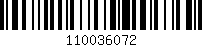
\includegraphics[scale=0.6]{Images/slj11-barcode.png}
\end{center}


               

%\thispagestyle{empty}

\begin{center}
    {\LARGE\bf Acknowledgements}
\end{center}

I would like to thank my supervisor Prof. Reyer Zwiggelaar for all of his help and support throughout this project. I would also like to thank Dr. Harry Strange for his guidance and supervision during the course of the project. His contributions to this project have been invaluable. In addition I would like to give special thanks Sam Nicholls for his data analysis and statistics knowledge. Finally I would like to thank my friends and family for their endless love and support throughout the project, with a special mention to Hannah Robarts who kept me sane. % Acknowledgements
%\thispagestyle{empty}

\begin{center}
    {\LARGE\bf Abstract}
\end{center}

Include an abstract for your project. This should be no more than 300 words.
                 % Abstract

\pagenumbering{roman}
\pagestyle{fancy}
\fancyhead{}
\fancyfoot[C]{\thepage}
\renewcommand{\headrulewidth}{0 pt}
\renewcommand{\chaptermark}[1]{\markboth{#1}{}}

\tableofcontents   
\newpage
\listoffigures
\newpage 
\listoftables
\newpage

% Set up page numbering
\pagenumbering{arabic}

\setchapterheaderfooter

% include the chapters
\chapter{Background \& Objectives}

\section{Mammography}
Breast cancer is the leading cause of dead among women world wide and is the most common form of cancer found in women \cite{siegel2014cancer}. Mammography is the analysis of female breast tissue through the use of X-ray radiology with the goal of producing high resolution images of the structure within the breast. The composition of the internal structure can then be used to permit earlier detection of breast cancer.

Qualitatively speaking the composition of breast tissue can be split into four distinct categories.
\subsection{Risk Assessment}
Mammograms provide a non-invasive means to assess the risk of a patient developing cancer. The general goal of a mammographic risk assessment is to evaluate the risk of patient having cancer. The composition of breast tissue can be categorised using the Breast Imaging Reporting And Data System (BI-RADS)\cite{american1998breast}. BI-RADS classifies mammograms based on the density of tissue (and therefore risk) in the mammogram.

\section{Features}
\subsection{Shape Features}
\subsection{Texture Features}

\section{Dimensionality Reduction}
\subsection{Linear}
\subsection{Non Linear}

\section{Visualisation}

\section{Analysis}

\section{Research Method}

%\addcontentsline{toc}{chapter}{Development Process}
\chapter{Experiment Methods}

\section{Overview}

\section{Techniques}
\subsection{Features}
\subsection{Dimensionality Reduction}
\subsection{Visualisation}

\section{Datasets}
\subsection{Synthetic Data}
\subsection{Real Data}

\section{Implementation}
\subsection{Languages}
\subsection{Libraries}
\chapter{Results and Conclusions}
\label{chap:results}

This chapter outlines the results of the experiments performed using the methods outlined in the preceding chapter. For each section in this chapter an brief comparison of the similarity exhibited by each feature is given followed by lower dimensional representations of the feature space. Finally, plots examining the quality of the visualisation are given.

Each of the experiments in this section used a single image from each patient in the full set of 360 images of both left, right and mediolateral oblique and craniocaudal views chosen at random. This meant was so as not to overrepresent a single patient for the real dataset. Therefore, 90 real mammograms in total were used for each experiment. The set of phantom mammograms used in this project consisted of 60 images but were divided into 6 groups corresponding to only a single ``case". Because of this limitation a single breast phantom from each case was selected at random to be included in the data used for the experiments, bringing the total number of images used in all experiments to 96.

Features extracted from both sets of images are compared using a two sample Kolmogorov-Smirnov (KS) test and are reported in the relevant section. The three dimensionality reduction algorithms were tested with each of the different feature sets and visualisations of the feature space in both 2 and 3 dimensions are shown for each.

Two different kinds of quality measure derived from the co-ranking matrix were computed for each of the visualisations shown in this section. The quality metrics used were trustworthiness \& continuity and the local continuity meta-criteria up to a neighbourhood of size $k=50$.

\section{Blob features} 
The results for the two sample KS test between the real and synthetic datasets for blob features detected over 10 scales are shown in table \ref{table:blob_features_ks}. An explanation of what each type of feature means can be found in section \ref{subsubsec:implementation-blob-features}. 2D projections of the blob feature space as produced by t-SNE, Isomap and locally linear embedding are shown in figures \ref{fig:blob_SNE_mapping}, \ref{fig:blob_iso_mapping}, and \ref{fig:blob_LLE_mapping} respectively. 

In each of the figures the real mammograms are shown as coloured dots and the breast phantoms are shown as coloured triangles. The labels corresponding to the colours used in each of the visualisations are the image's BIRADS class (in the case of real mammograms) or the volumetric breast density (VBD) (in the case of breast phantoms).

Generally speaking the phantom mammograms are shown to be very different from the real mammograms features used. The size of blobs detected in the phantom mammograms are generally larger and contain far fewer small scale blobs when compared to real mammograms. This is reflected in the projections for this feature space. 

In the t-SNE projections it can be seen that all of the phantom blobs, regardless of VBD, are grouped towards the bottom of the distribution which contains a relatively high proportion of BIRADS risk class 3 \& 4 images. The projections produced by Isomap and LLE generally separate the breast phantoms for the original data more than with t-SNE. Several of the real mammograms with features that match those of the breast phantoms are also interspersed with the phantom mammograms. This can be seen best in the 2D projection produced by Isomap in figure \ref{fig:blob_iso_mapping}. These real mammograms are ones which tend to have a higher number of larger blobs detected than real mammograms in general.

\begin{table}[H]
\label{table:blob_features_ks}
\centering
\primitiveinput{tables/blob_features_ks}
\caption{Comparison of the Kolmogorov-Smirnov test results for each feature generated from the radii of blobs detected in an image between real and phantom mammograms.}
\end{table}

The quality evaluation for each of the visualisations are shown in figures \ref{fig:TC_2d_blobs}, \ref{fig:TC_3d_blobs}, and \ref{fig:LCMC_blobs}. The quality metrics shown in these figures suggest that the 2D visualisation produced by Isomap is the most trustworthy, but t-SNE has better continuity. In the case of the 3D projections Isomap provides a better visualisation with it topping both criteria. For both projections Isomap show better performance in terms of the LCMC, but is overtaken for larger values of $k$ in 2D projections by t-SNE and in 3D projections by LLE. 

\clearpage

\begin{figure}[H]
	\centering
	\subfigure{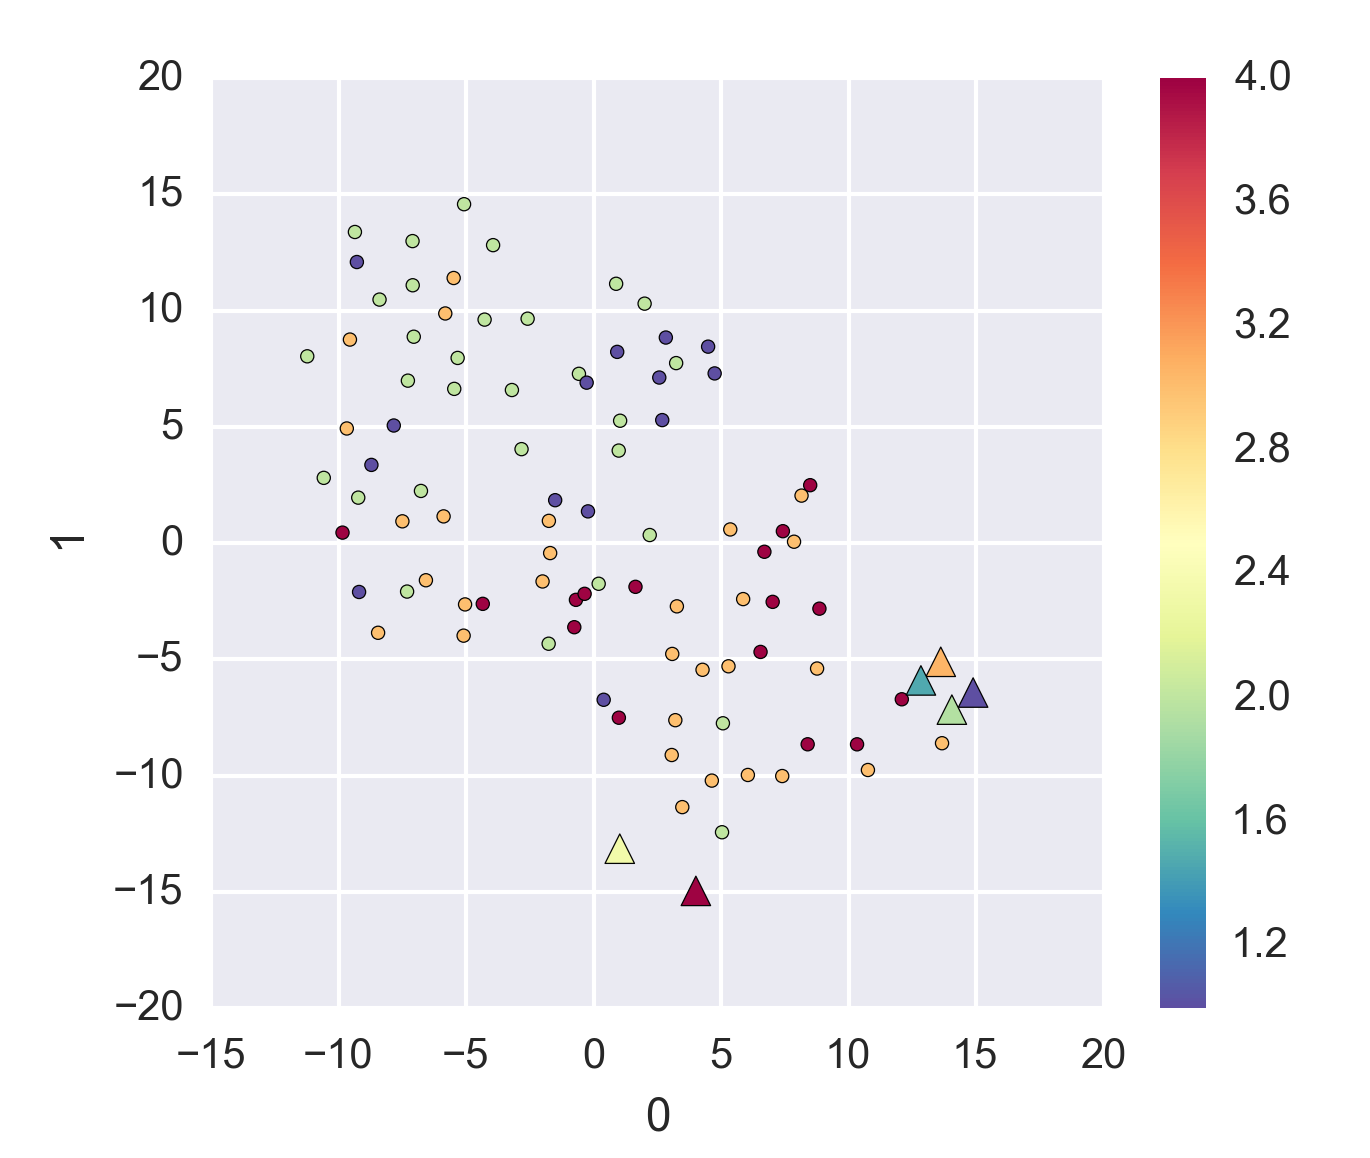
\includegraphics[width=0.4\textwidth]{figures/mappings/blob_SNE_mapping_2d.png}}
	\subfigure{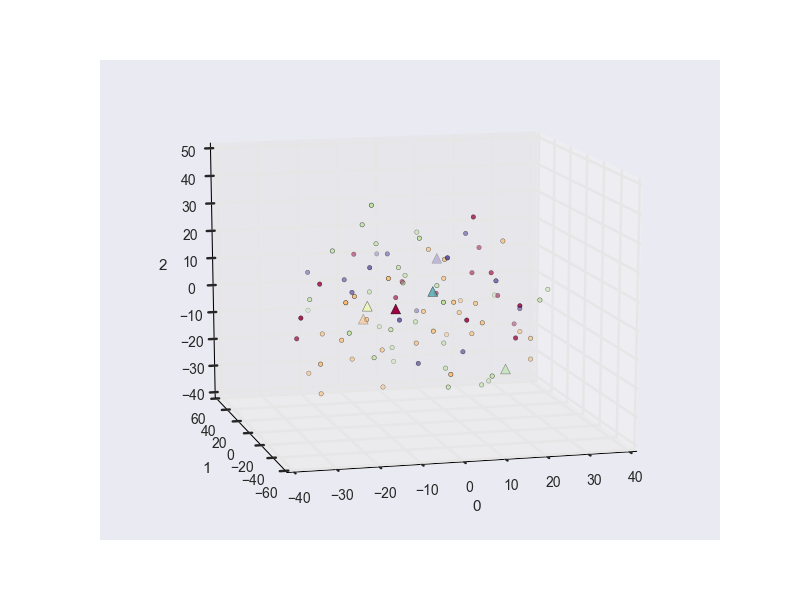
\includegraphics[width=0.49\textwidth]{figures/mappings/blob_SNE_mapping_3d.png}}
	\caption{2D \& 3D projections of the blob feature space produced by the t-SNE algorithm with a learning rate of 200 and perplexity of 20.}\label{fig:blob_SNE_mapping}
\end{figure}

\begin{figure}[H]
	\centering
	\subfigure{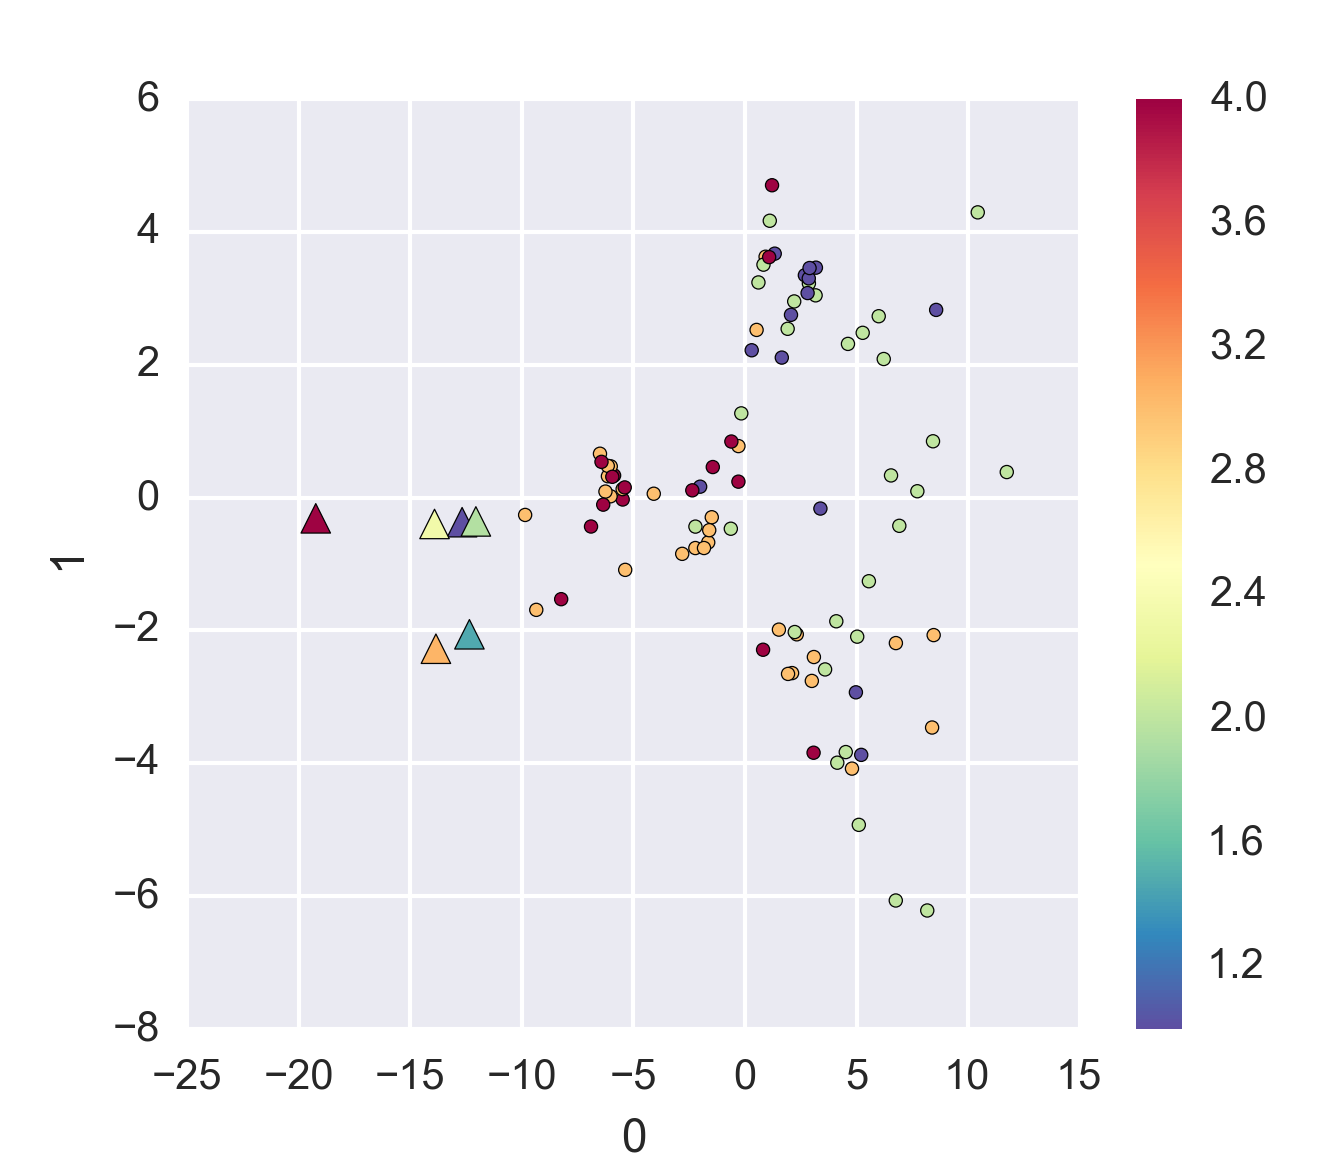
\includegraphics[width=0.4\textwidth]{figures/mappings/blob_iso_mapping_2d.png}}
	\subfigure{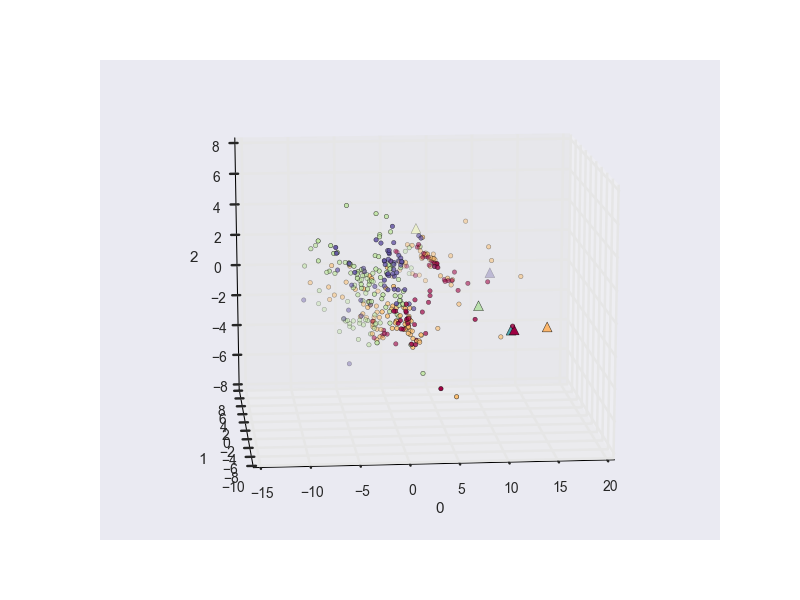
\includegraphics[width=0.49\textwidth]{figures/mappings/blob_iso_mapping_3d.png}}
	\caption{2D \& 3D projections of the blob feature space  produced by the Isomap algorithm with 4 neighbours.}\label{fig:blob_iso_mapping}
\end{figure}

\begin{figure}[H]
	\centering
	\subfigure{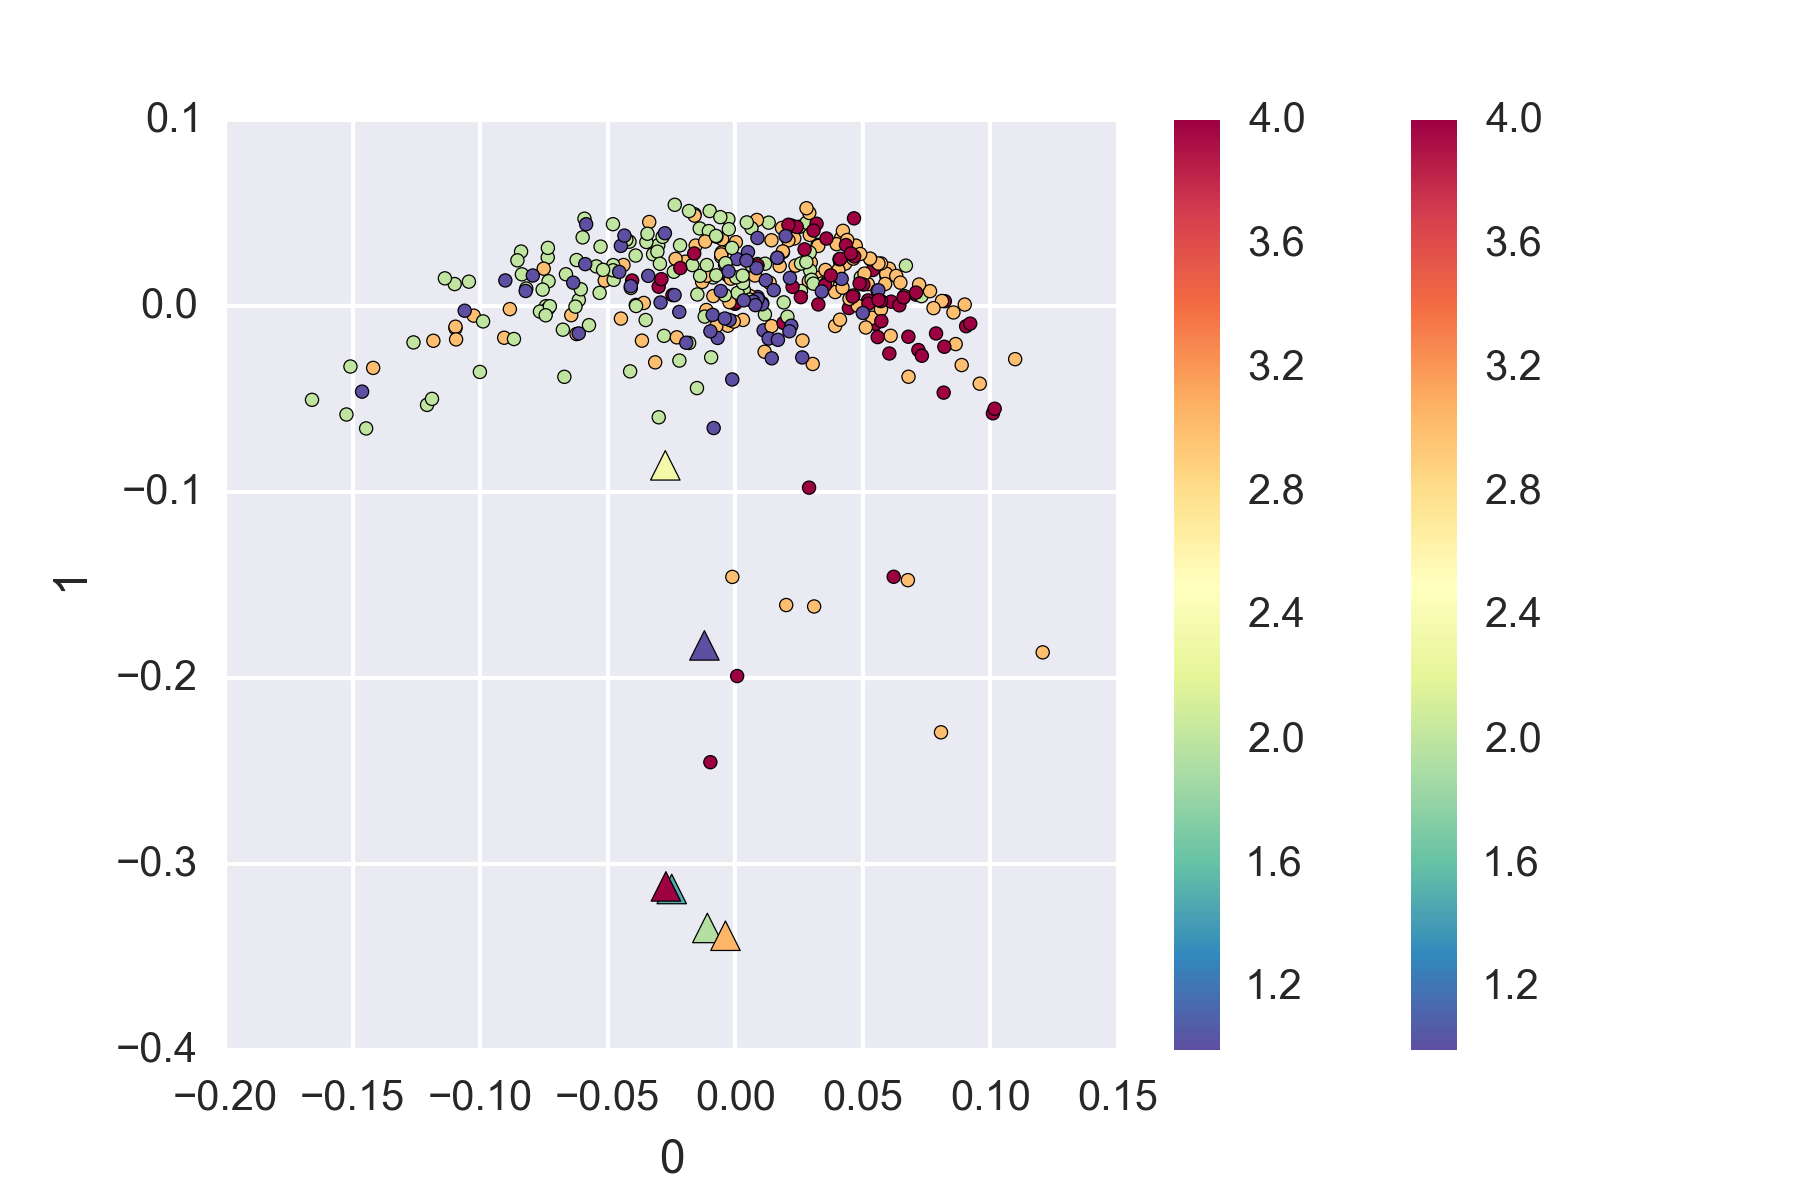
\includegraphics[width=0.4\textwidth]{figures/mappings/blob_lle_mapping_2d.png}}
	\subfigure{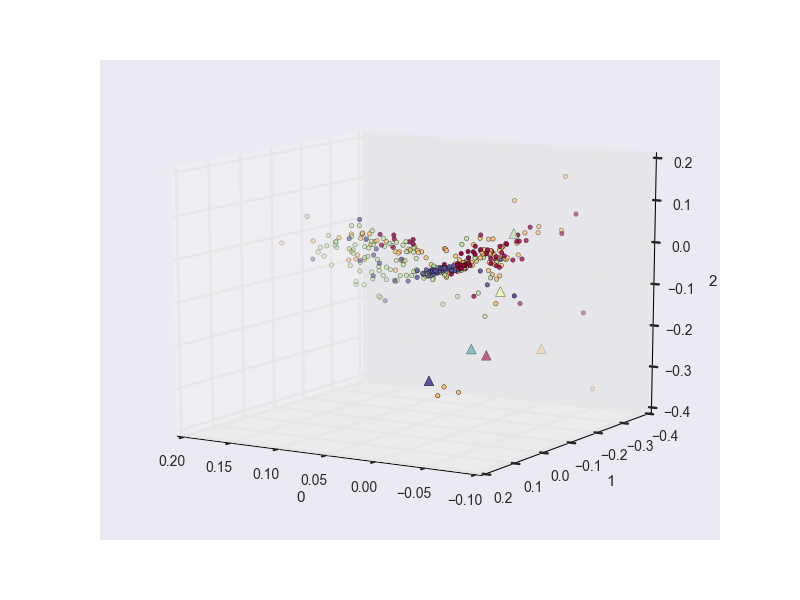
\includegraphics[width=0.49\textwidth]{figures/mappings/blob_lle_mapping_3d.png}}
	\caption{2D \& 3D projections of the blob feature space produced by the LLE algorithm with 4 neighbours.}\label{fig:blob_LLE_mapping}
\end{figure}
\clearpage

\clearpage
\begin{figure}[H]
	\centering
	\subfigure{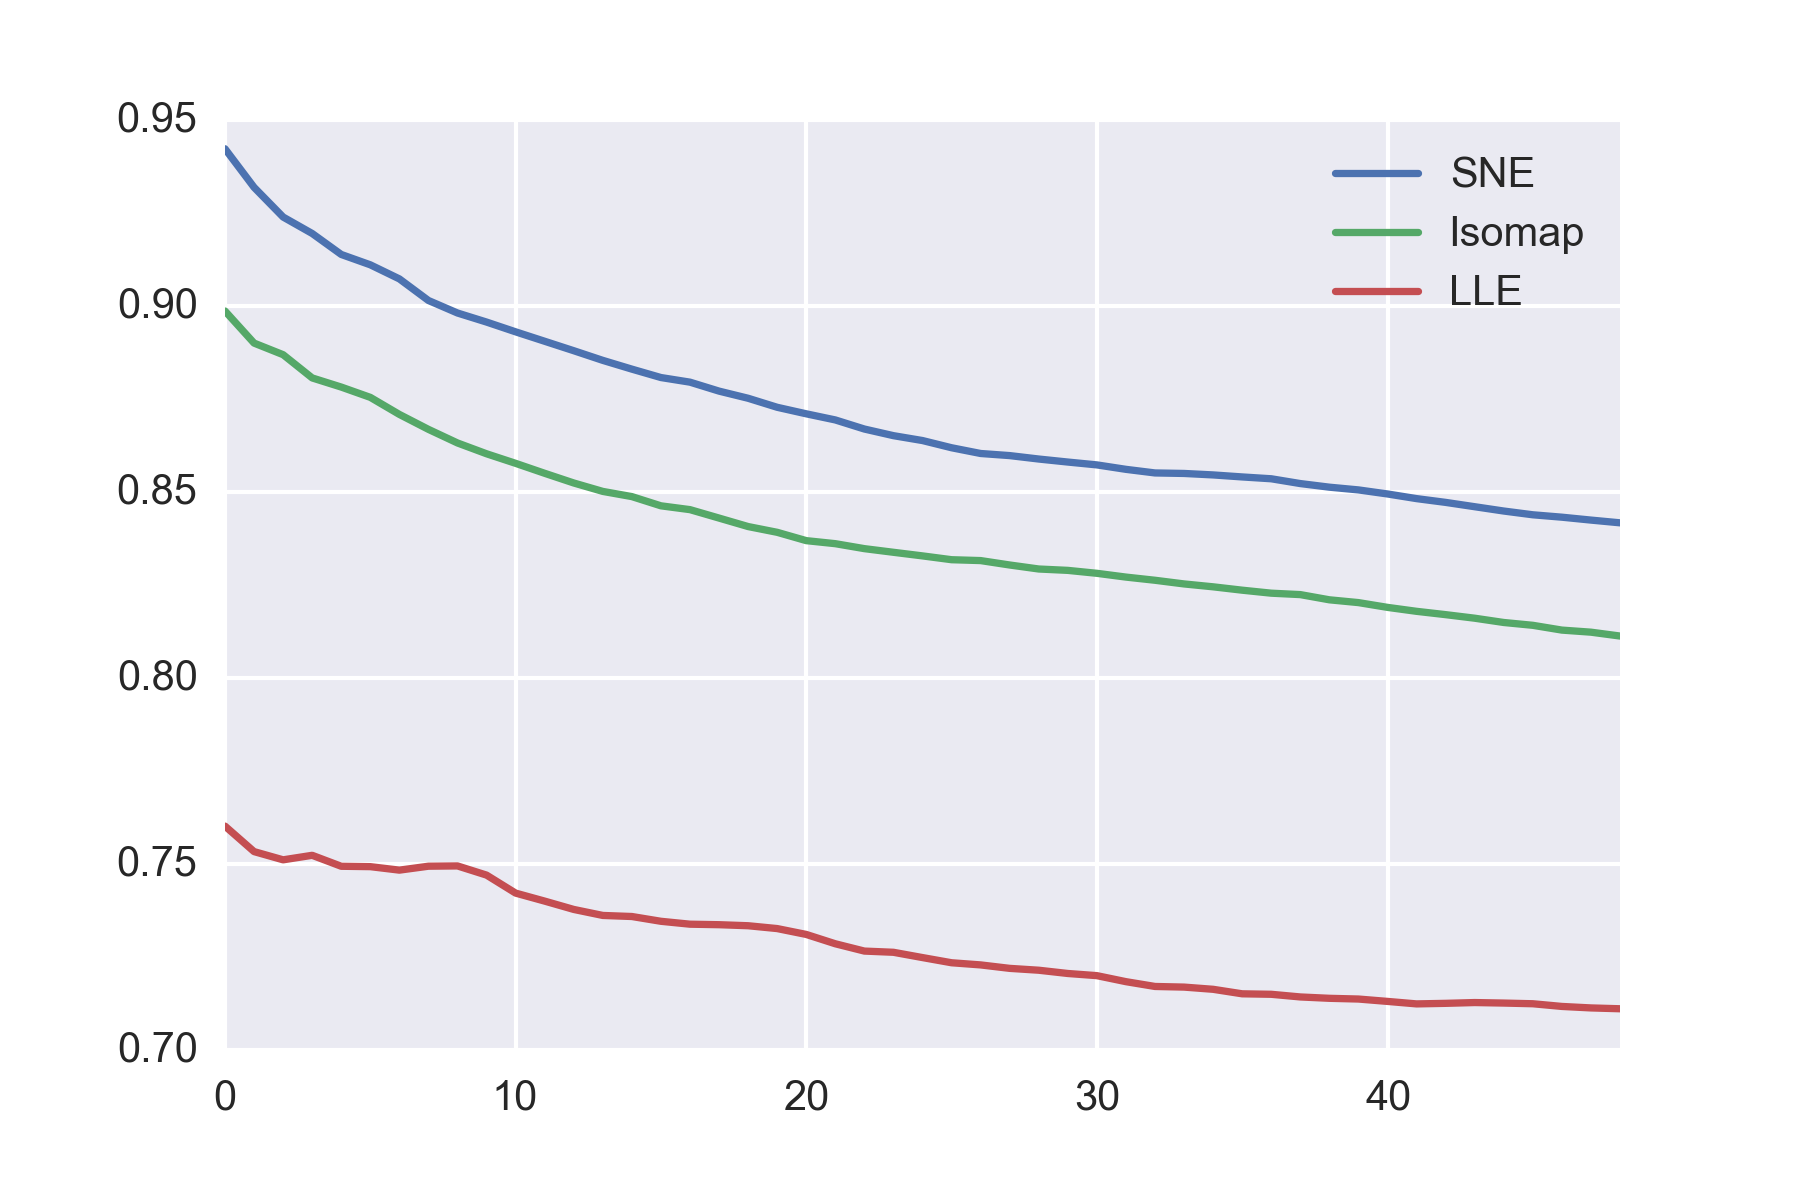
\includegraphics[width=0.49\textwidth]{figures/quality_measures/blob_trustworthiness_2d.png}}
	\subfigure{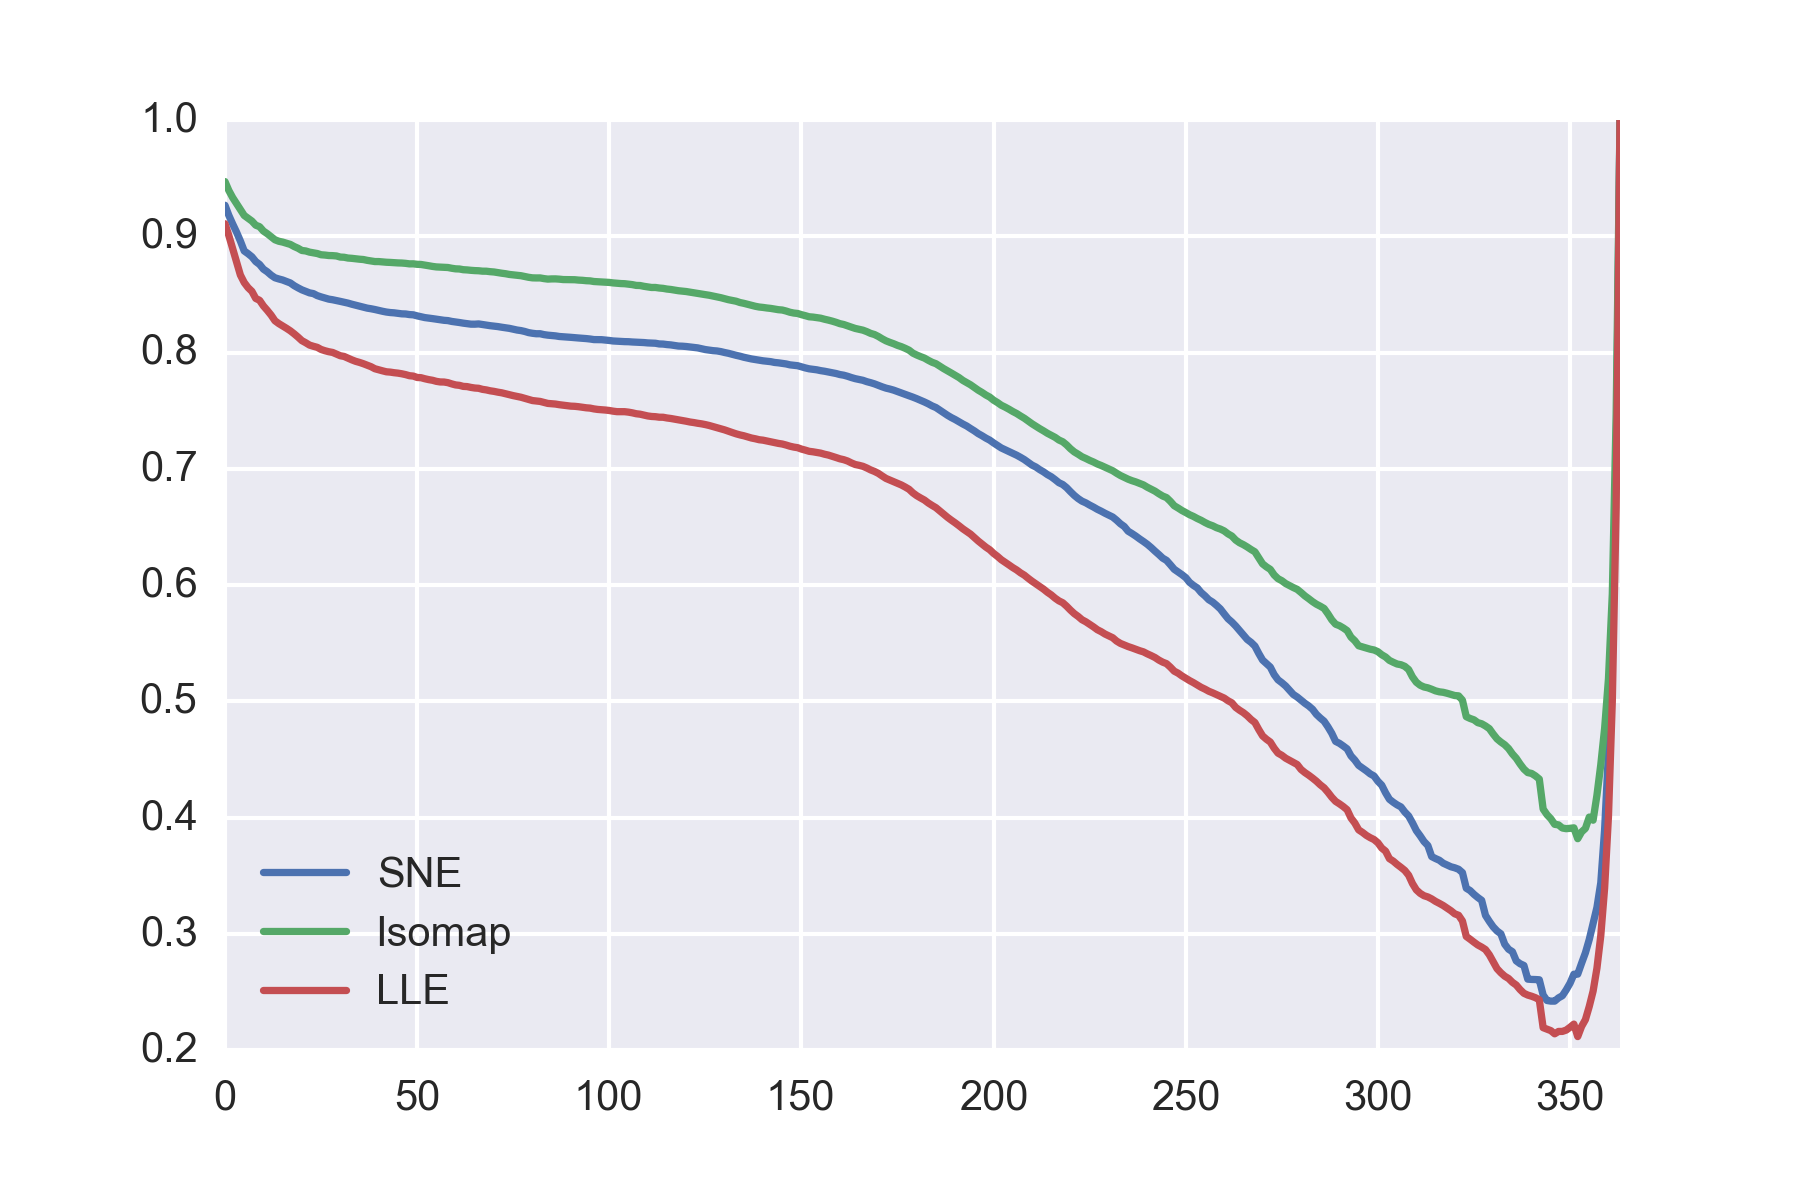
\includegraphics[width=0.49\textwidth]{figures/quality_measures/blob_continuity_2d.png}}
	\caption{Trustworthiness (left) and continuity (right) of the 2D projections produced from blob features.}\label{fig:TC_2d_blobs}
\end{figure}

\begin{figure}[H]
	\centering
	\subfigure{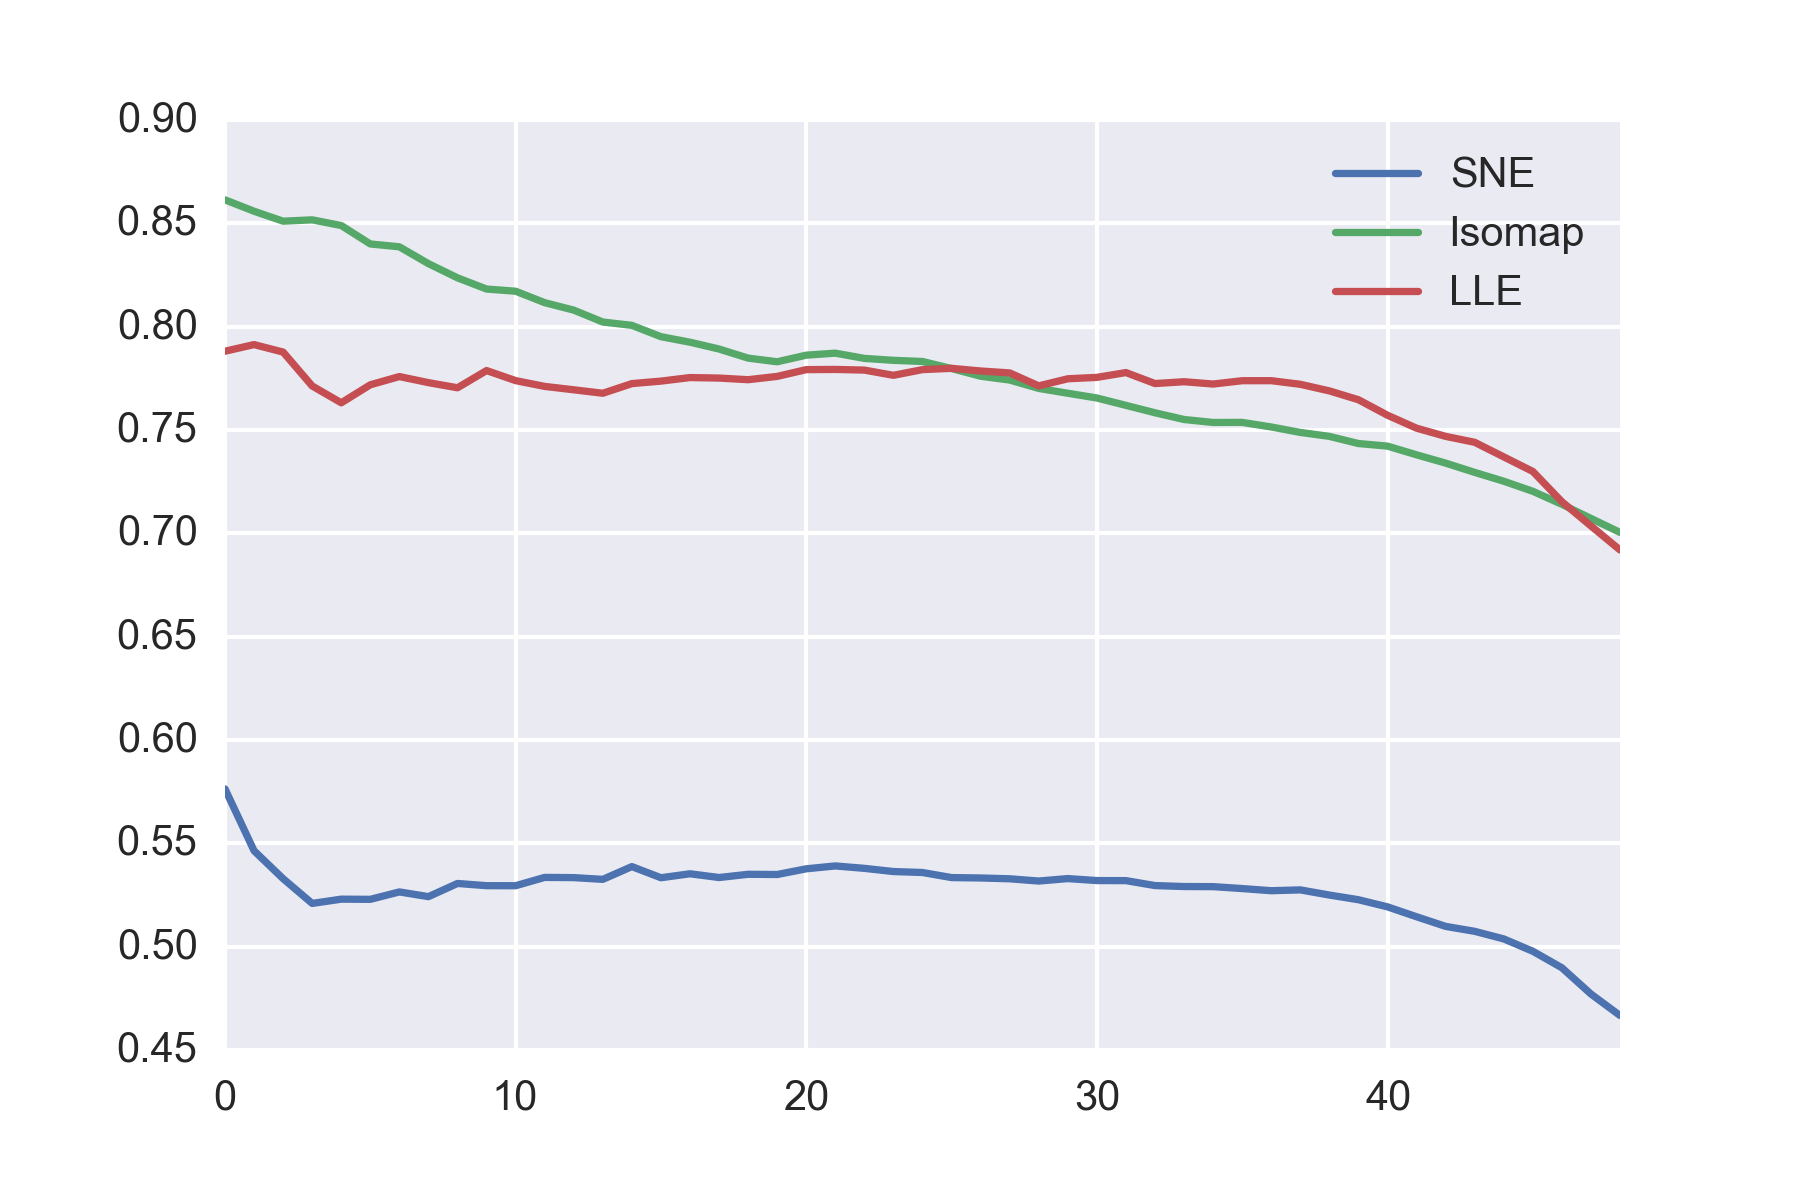
\includegraphics[width=0.49\textwidth]{figures/quality_measures/blob_trustworthiness_3d.png}}
	\subfigure{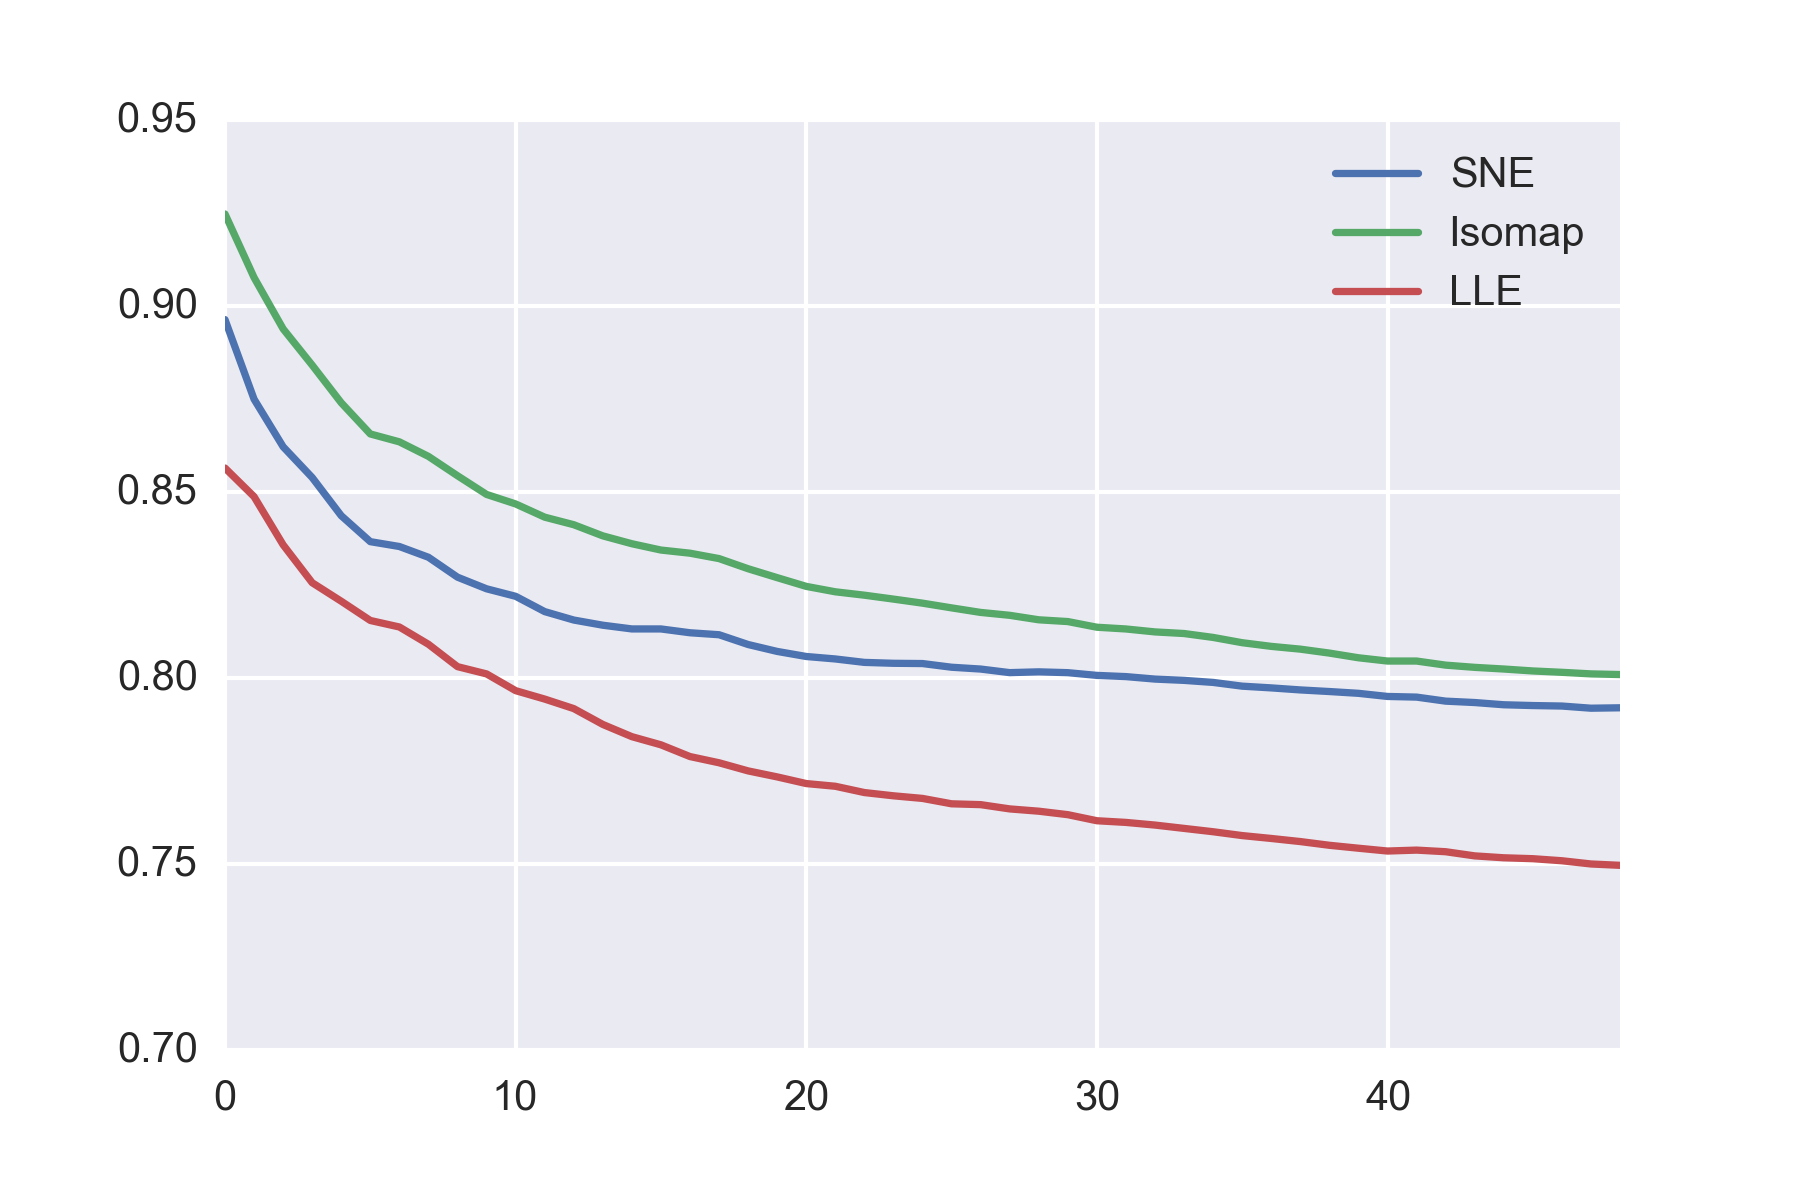
\includegraphics[width=0.49\textwidth]{figures/quality_measures/blob_continuity_3d.png}}
	\caption{Trustworthiness (left) and continuity (right) of the 3D projections produced from blob features.}\label{fig:TC_3d_blobs}
\end{figure}

\begin{figure}[H]
	\centering
	\subfigure{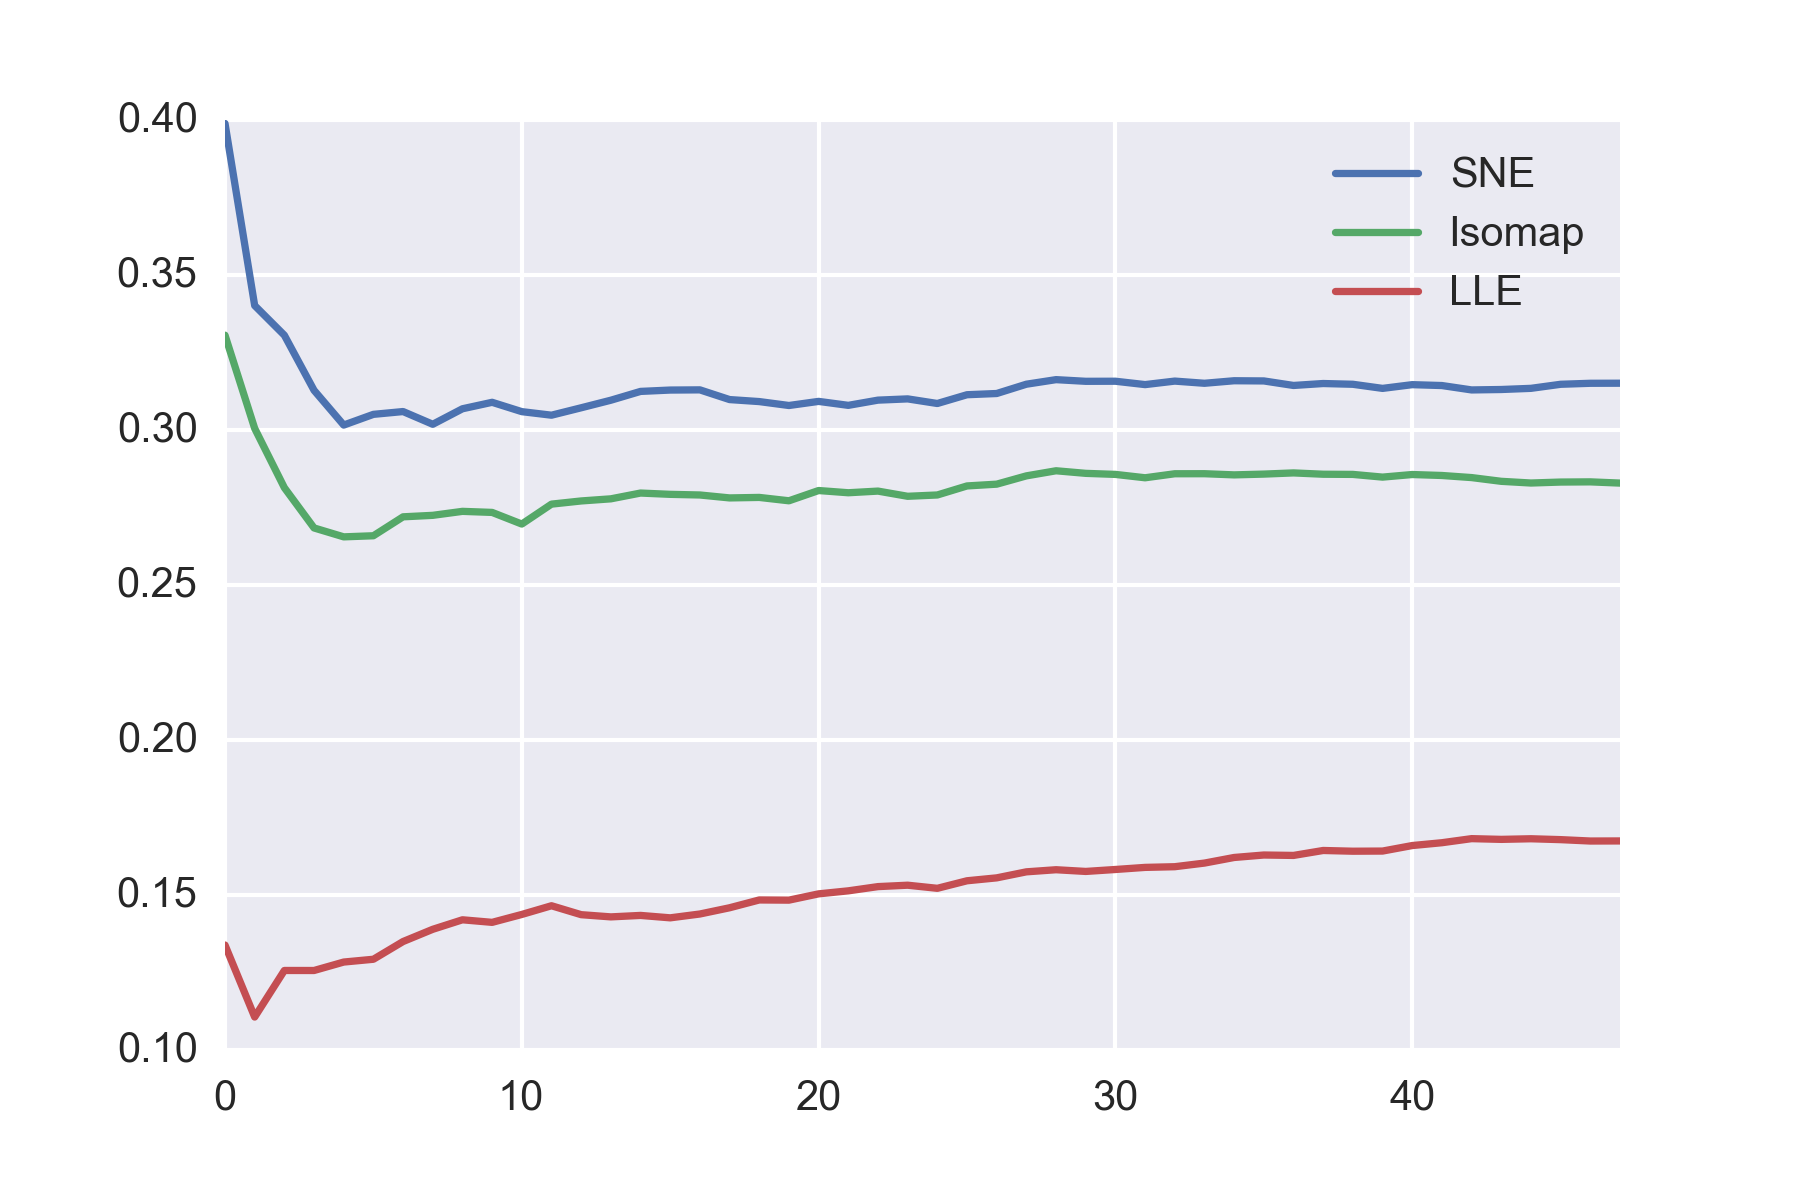
\includegraphics[width=0.49\textwidth]{figures/quality_measures/blob_lcmc_2d.png}}
	\subfigure{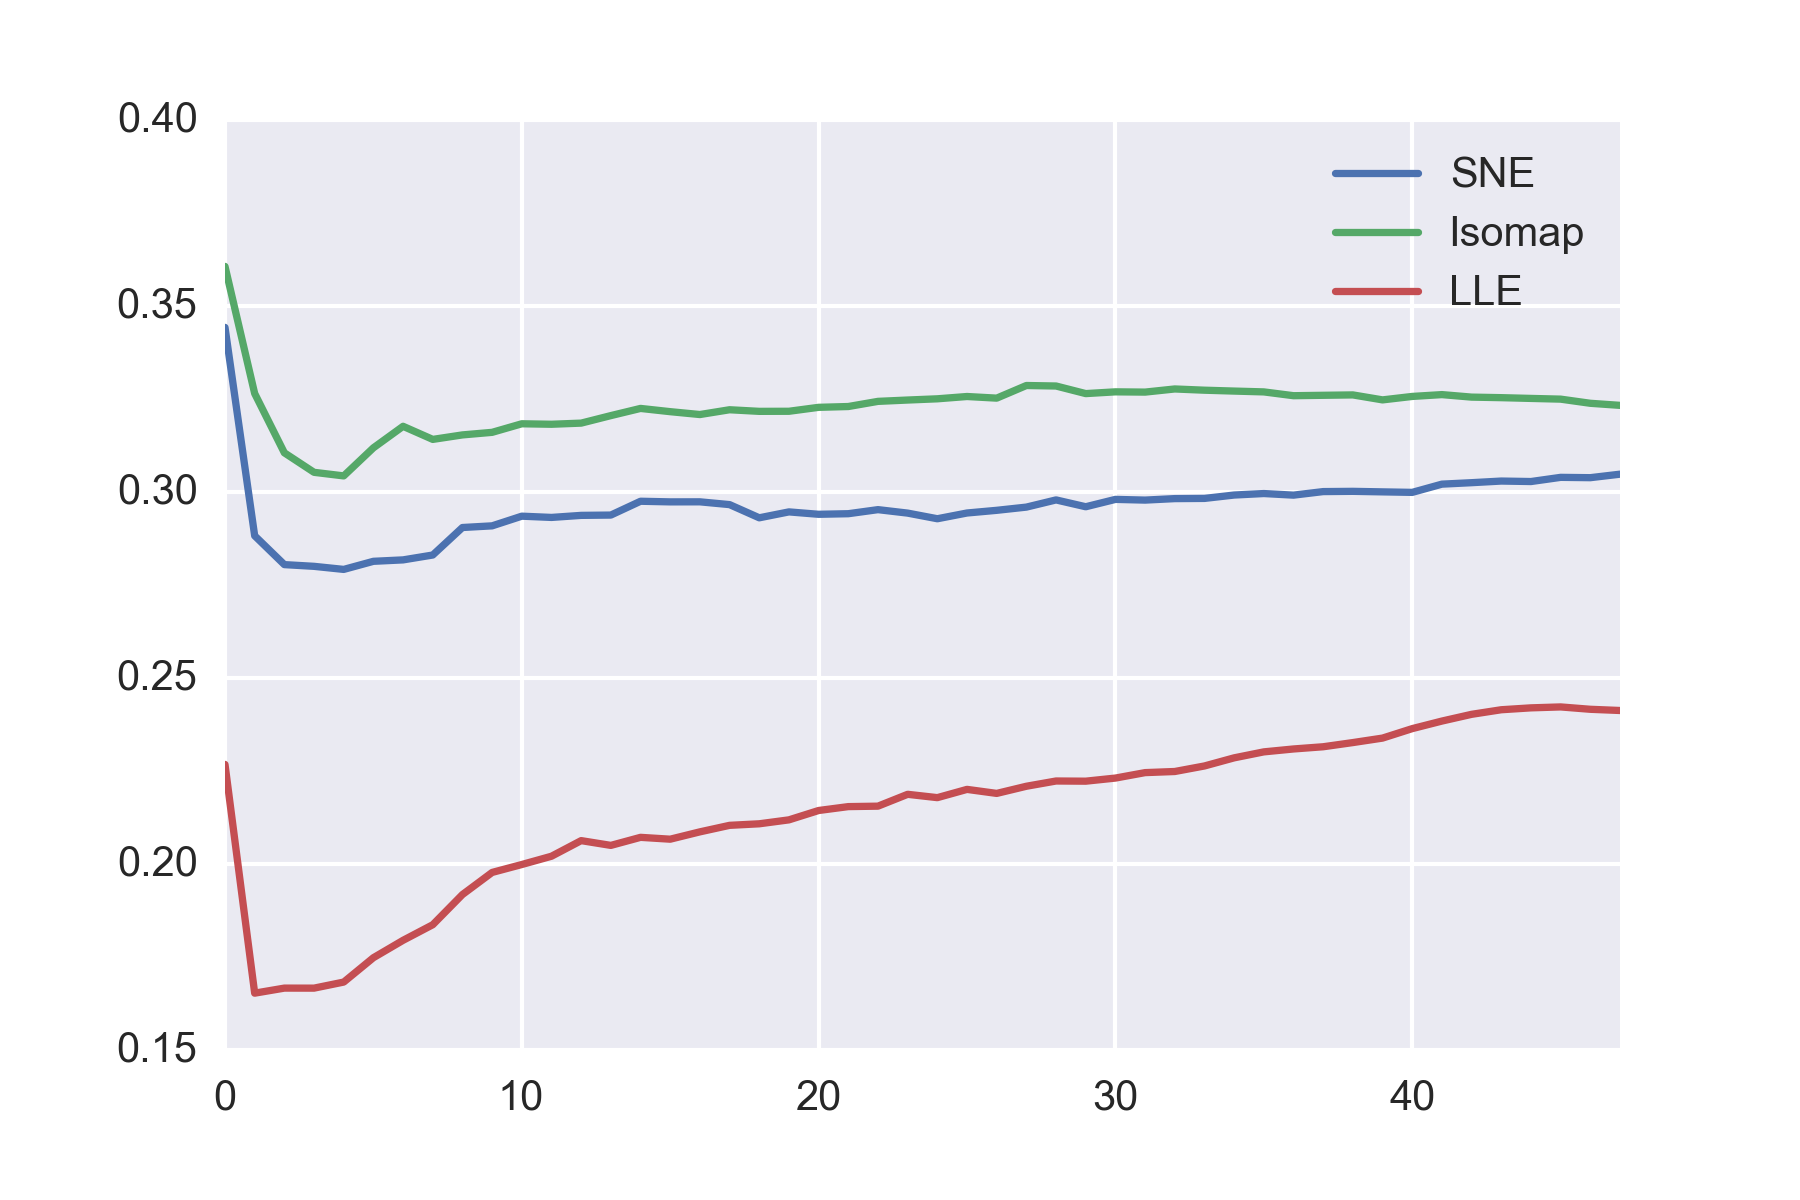
\includegraphics[width=0.49\textwidth]{figures/quality_measures/blob_lcmc_3d.png}}
	\caption{LCMC of both the 2D projection (left) and 3D projection (right) of the feature space for blobs.}\label{fig:LCMC_blobs}
\end{figure}
\clearpage

\subsection{Line features}
Results for the KS two sample test between the two feature spaces can be seen in table \ref{table:line_features_ks}. Again, as with blobs, the distributions for real and synthetic mammograms are not in particularly good agreement according to the test. 2D and 3D projections for the line feature space for each of the three different dimensionality reduction algorithms are shown in figures \ref{fig:line_SNE_mapping}, \ref{fig:line_iso_mapping}, and \ref{fig:line_LLE_mapping} respectively.
 
Note that in these results the value of the min area feature was removed. When using the min area feature all projections would produce two clusters. One smaller cluster would be created containing which contained blobs where the min area was much larger than the rest of the dataset. This is most likely caused by a thresholding issue causing some unwanted smaller lines to be retained for some of the images.

\begin{table}[H]
\label{table:line_features_ks}
\centering
\primitiveinput{tables/line_features_ks}
\caption{Comparison of the Kolmogorov-Smirnov test results for each feature generated from the area of lines detected in an image between real and phantom mammograms.}
\end{table}

The t-SNE projection shows that there is a general transition from images which contain a high mean area of linear structure on the bottom right towards images which have a lower mean area in the top left. In terms of BIRADS risk it can be seen that very low and very high risk classes are grouped towards the bottom right, reflecting that less liner structure is detected using the orientated bins method in low risk classes (because there's very little dense structure present) and high risk classes (because dense areas are mostly large, homogenous blobs not linear structure). As can be clearly seen from the visualisation the synthetic images are grouped towards the lower end reflecting the smaller size of the linear structures detected. The 3D version produced by t-SNE produced a far worse projection with less visible structure.

The projections produced by Isomap produce more clearly show the synthetics begin grouped in with the very low/high risk blobs towards the left of the mapping. For LLE the majority of the blobs are pushed away from the main body of the mapping and closer to some of the outliers of the real mammograms.

Examination of the three quality criteria show that Isomap produces better projections across both the 2D and 2D visualisations. t-SNE produced a 2D mapping which was comparable to Isomap in terms of trustworthiness and continuity, and LCMC. However in the case of the 3D case this was radically worse over all measures.

\begin{figure}[H]
	\centering
	\subfigure{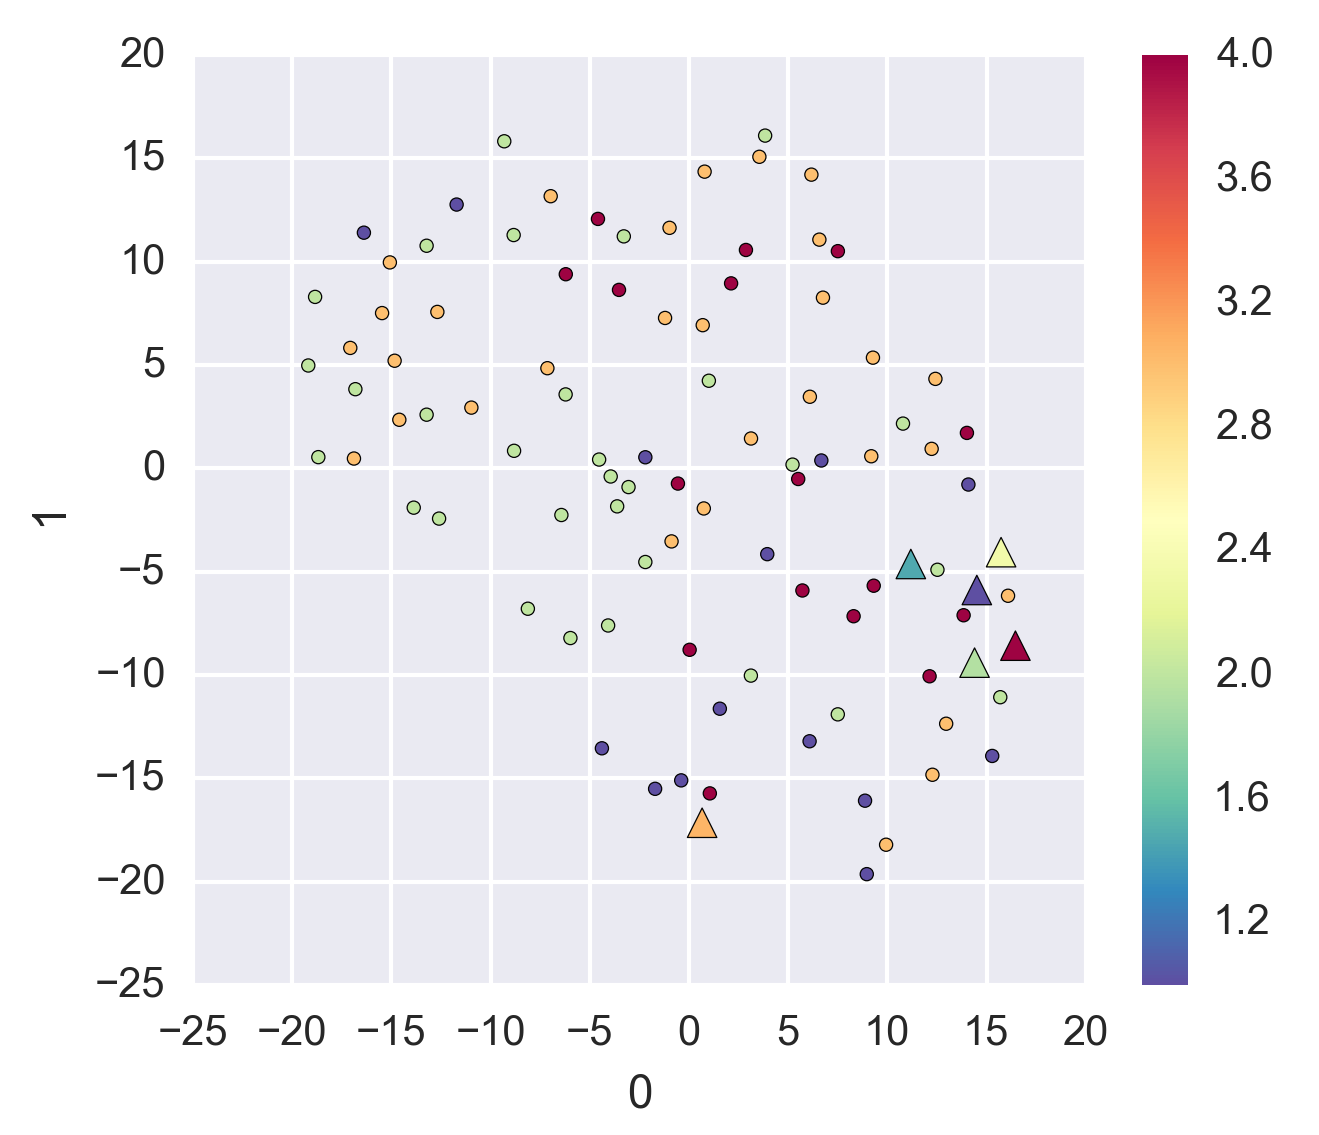
\includegraphics[width=0.4\textwidth]{figures/mappings/line_SNE_mapping_2d.png}}
	\subfigure{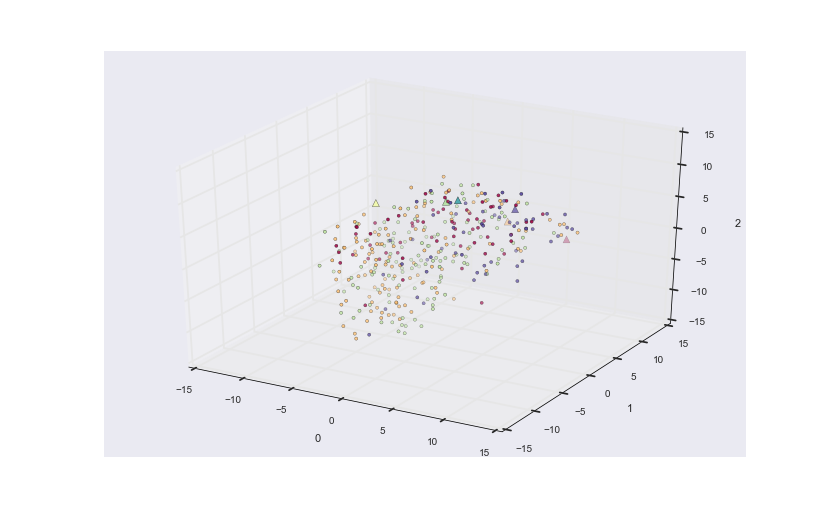
\includegraphics[width=0.49\textwidth]{figures/mappings/line_SNE_mapping_3d.png}}
	\caption{2D \& 3D projections of the line feature space produced by the t-SNE algorithm with a learning rate of 200 and perplexity of 20.}\label{fig:line_SNE_mapping}
\end{figure}

\begin{figure}[H]
	\centering
	\subfigure{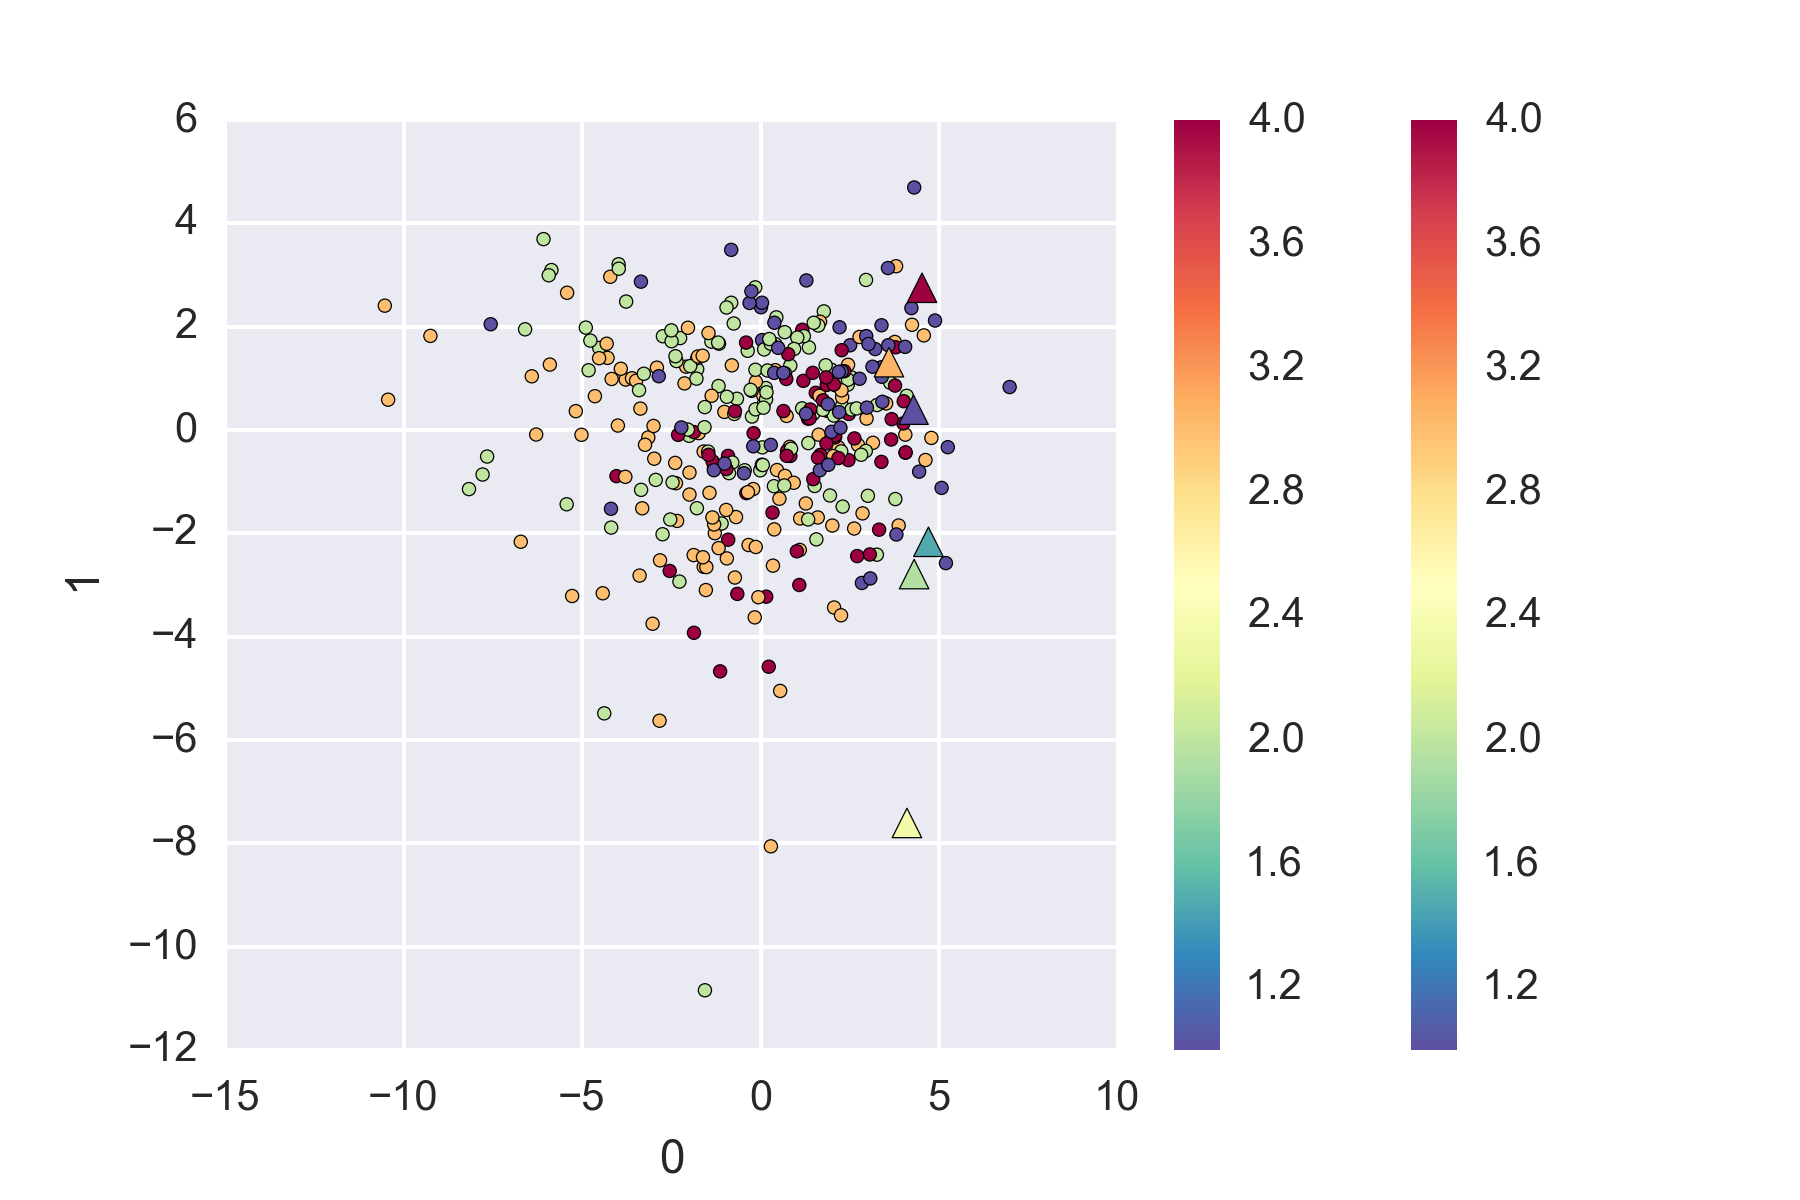
\includegraphics[width=0.4\textwidth]{figures/mappings/line_iso_mapping_2d.png}}
	\subfigure{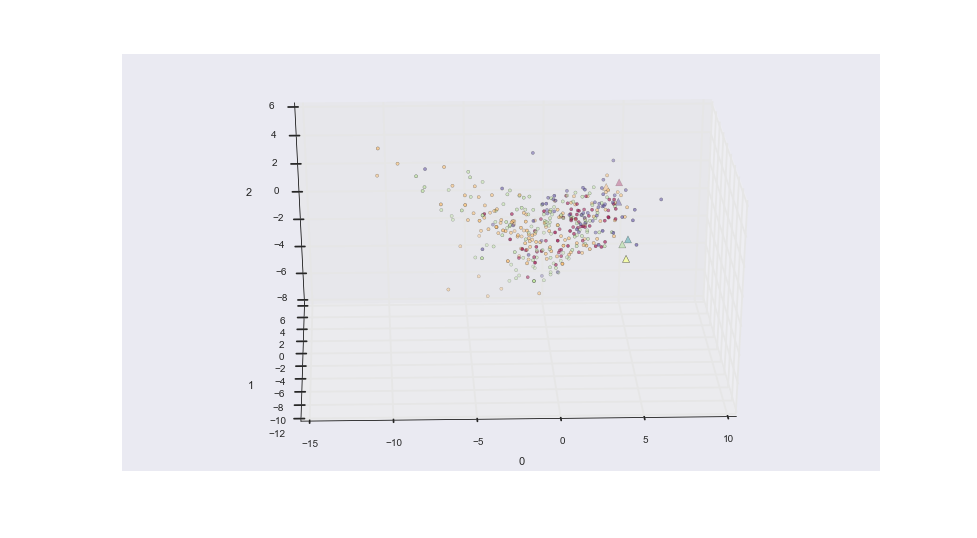
\includegraphics[width=0.49\textwidth]{figures/mappings/line_iso_mapping_3d.png}}
	\caption{2D \& 3D projections of the line feature space  produced by the Isomap algorithm with 4 neighbours.}\label{fig:line_iso_mapping}
\end{figure}

\begin{figure}[H]
	\centering
	\subfigure{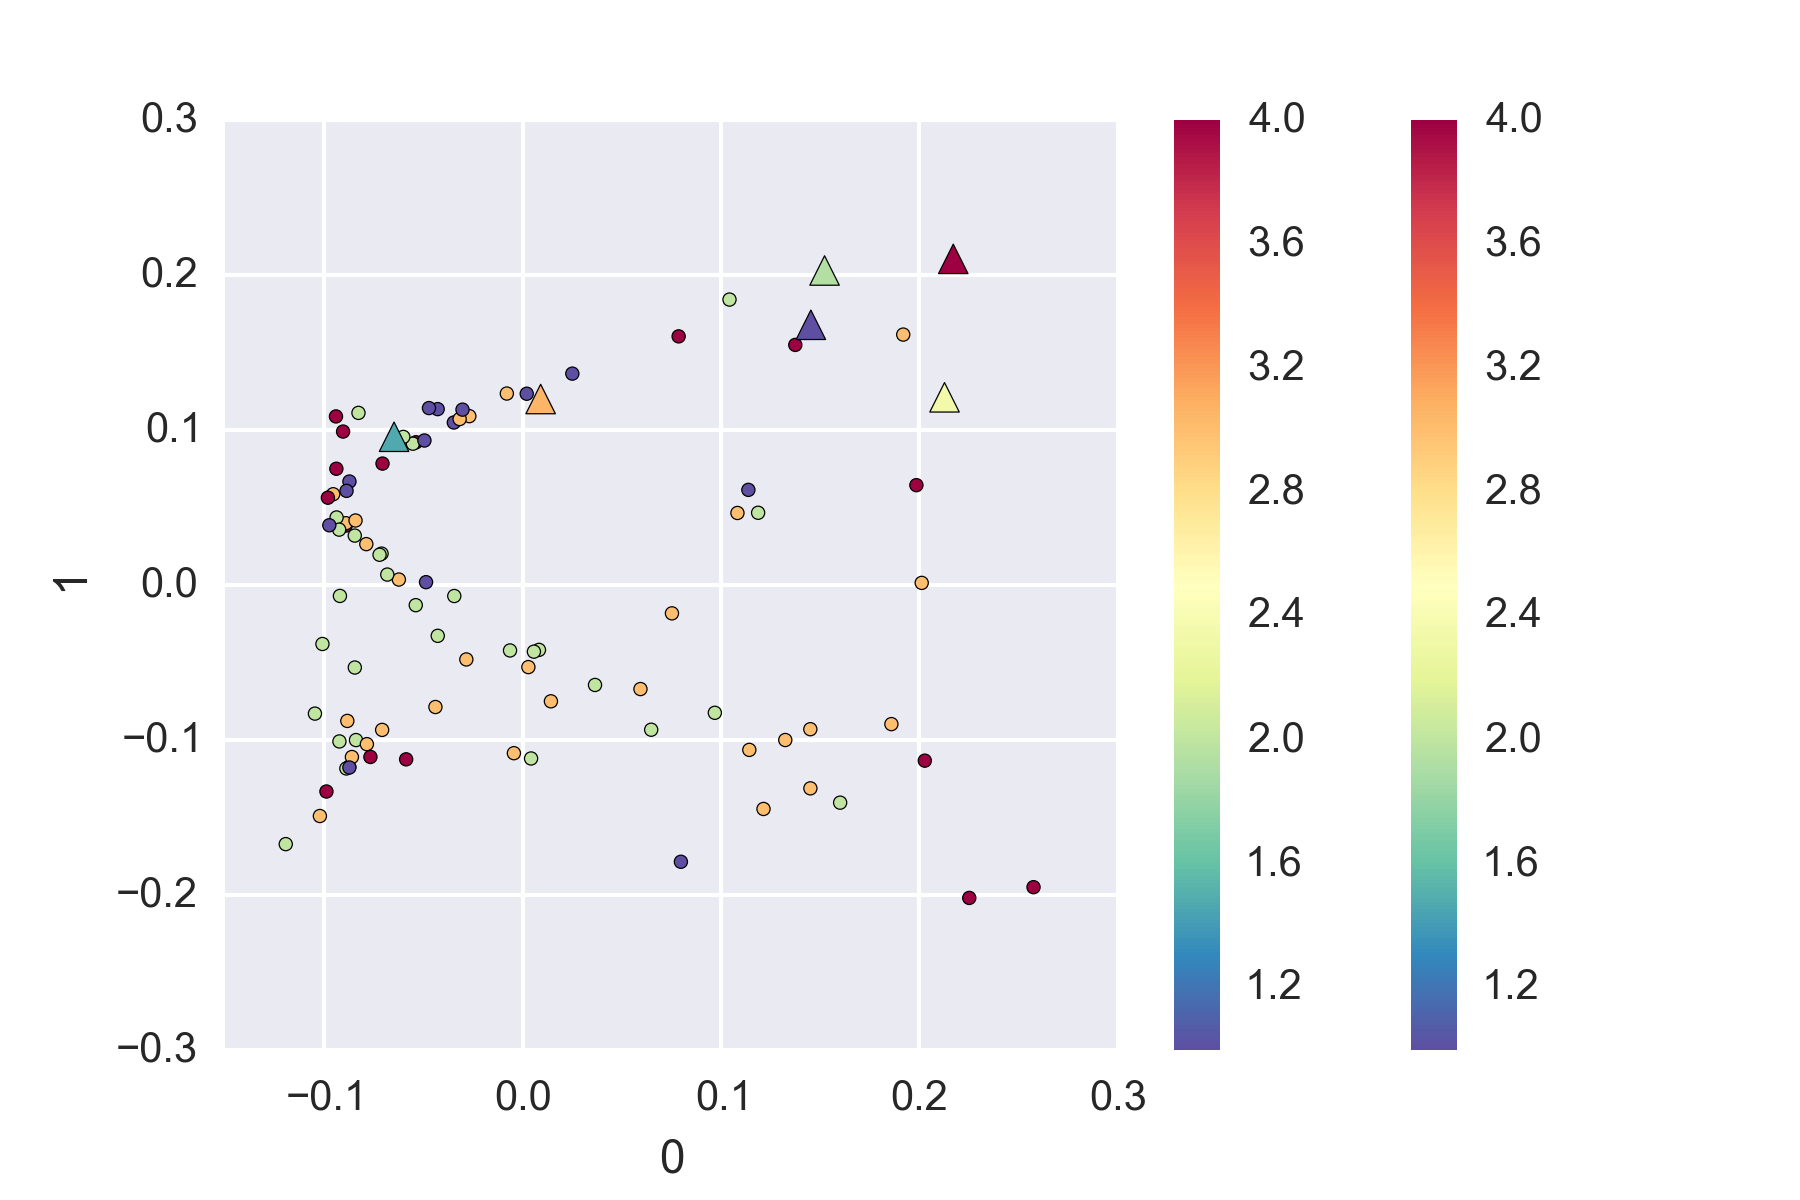
\includegraphics[width=0.4\textwidth]{figures/mappings/line_lle_mapping_2d.png}}
	\subfigure{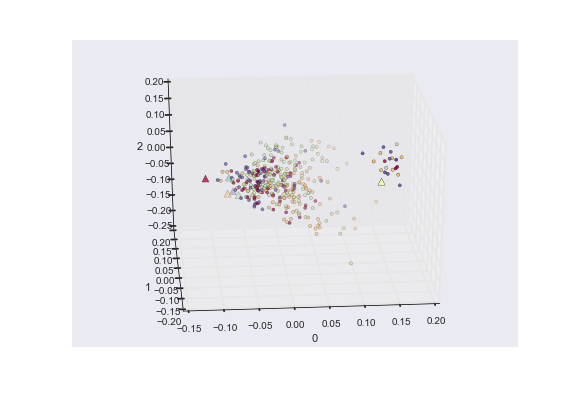
\includegraphics[width=0.49\textwidth]{figures/mappings/line_lle_mapping_3d.png}}
	\caption{2D \& 3D projections of the line feature space produced by the LLE algorithm with 4 neighbours.}\label{fig:line_LLE_mapping}
\end{figure}
\clearpage

\clearpage
\begin{figure}[H]
	\centering
	\subfigure{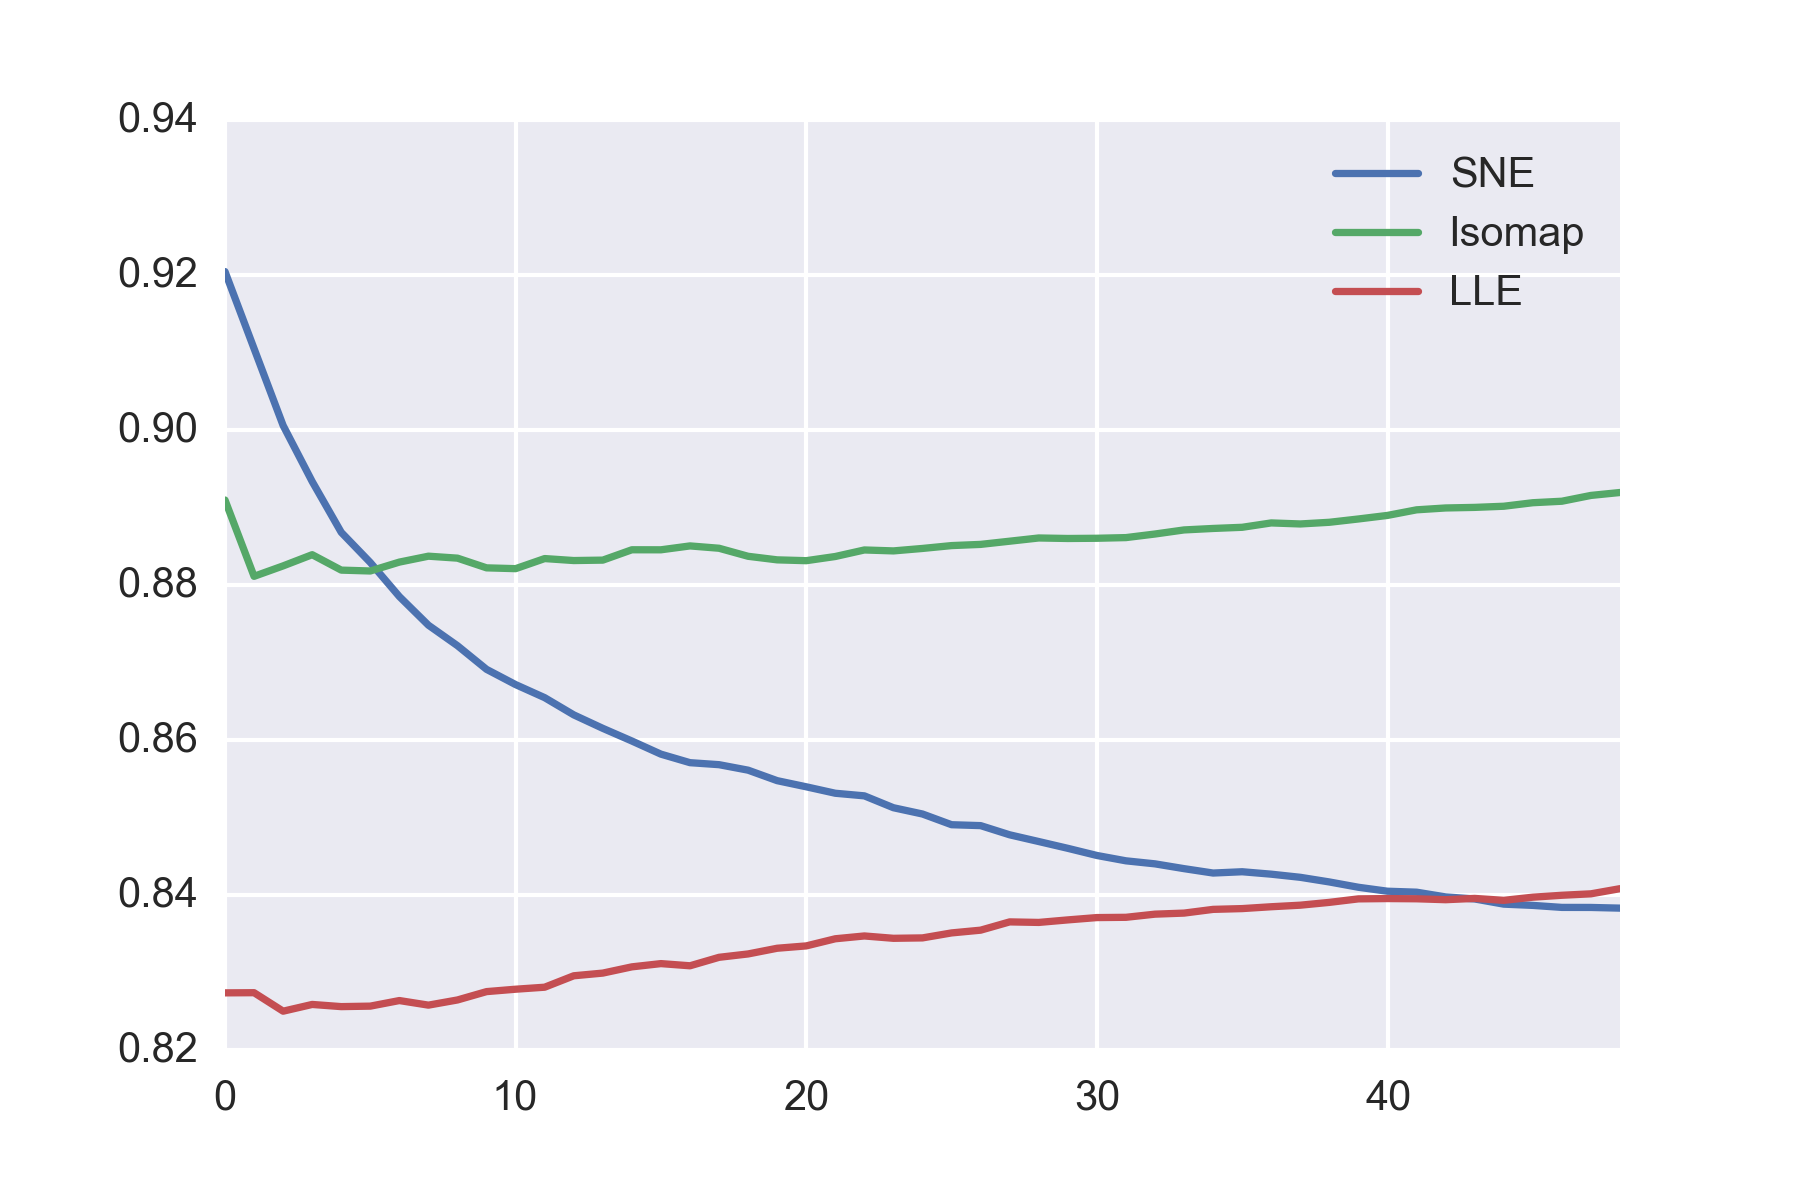
\includegraphics[width=0.49\textwidth]{figures/quality_measures/line_trustworthiness_2d.png}}
	\subfigure{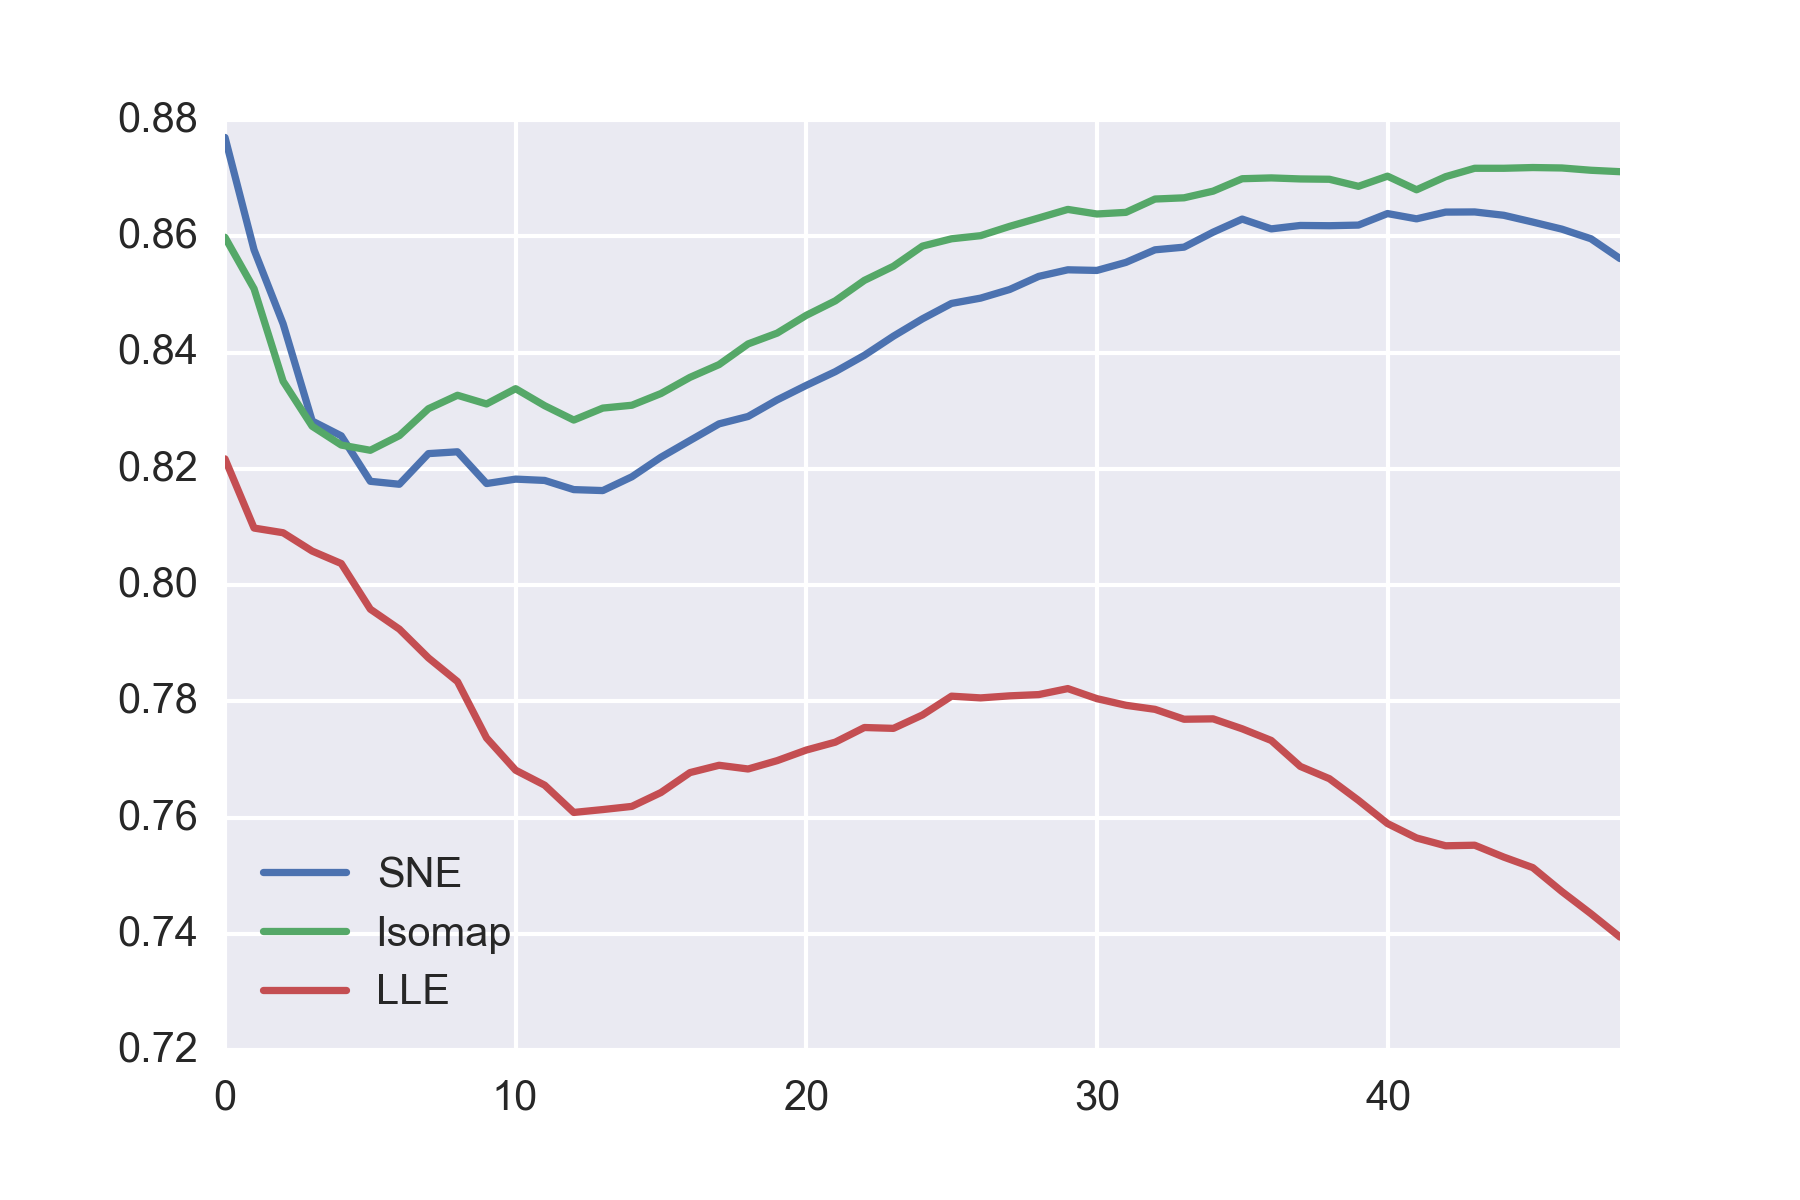
\includegraphics[width=0.49\textwidth]{figures/quality_measures/line_continuity_2d.png}}
	\caption{Trustworthiness (left) and continuity (right) of the 2D projections produced from line features.}\label{fig:TC_2d_lines}
\end{figure}

\begin{figure}[H]
	\centering
	\subfigure{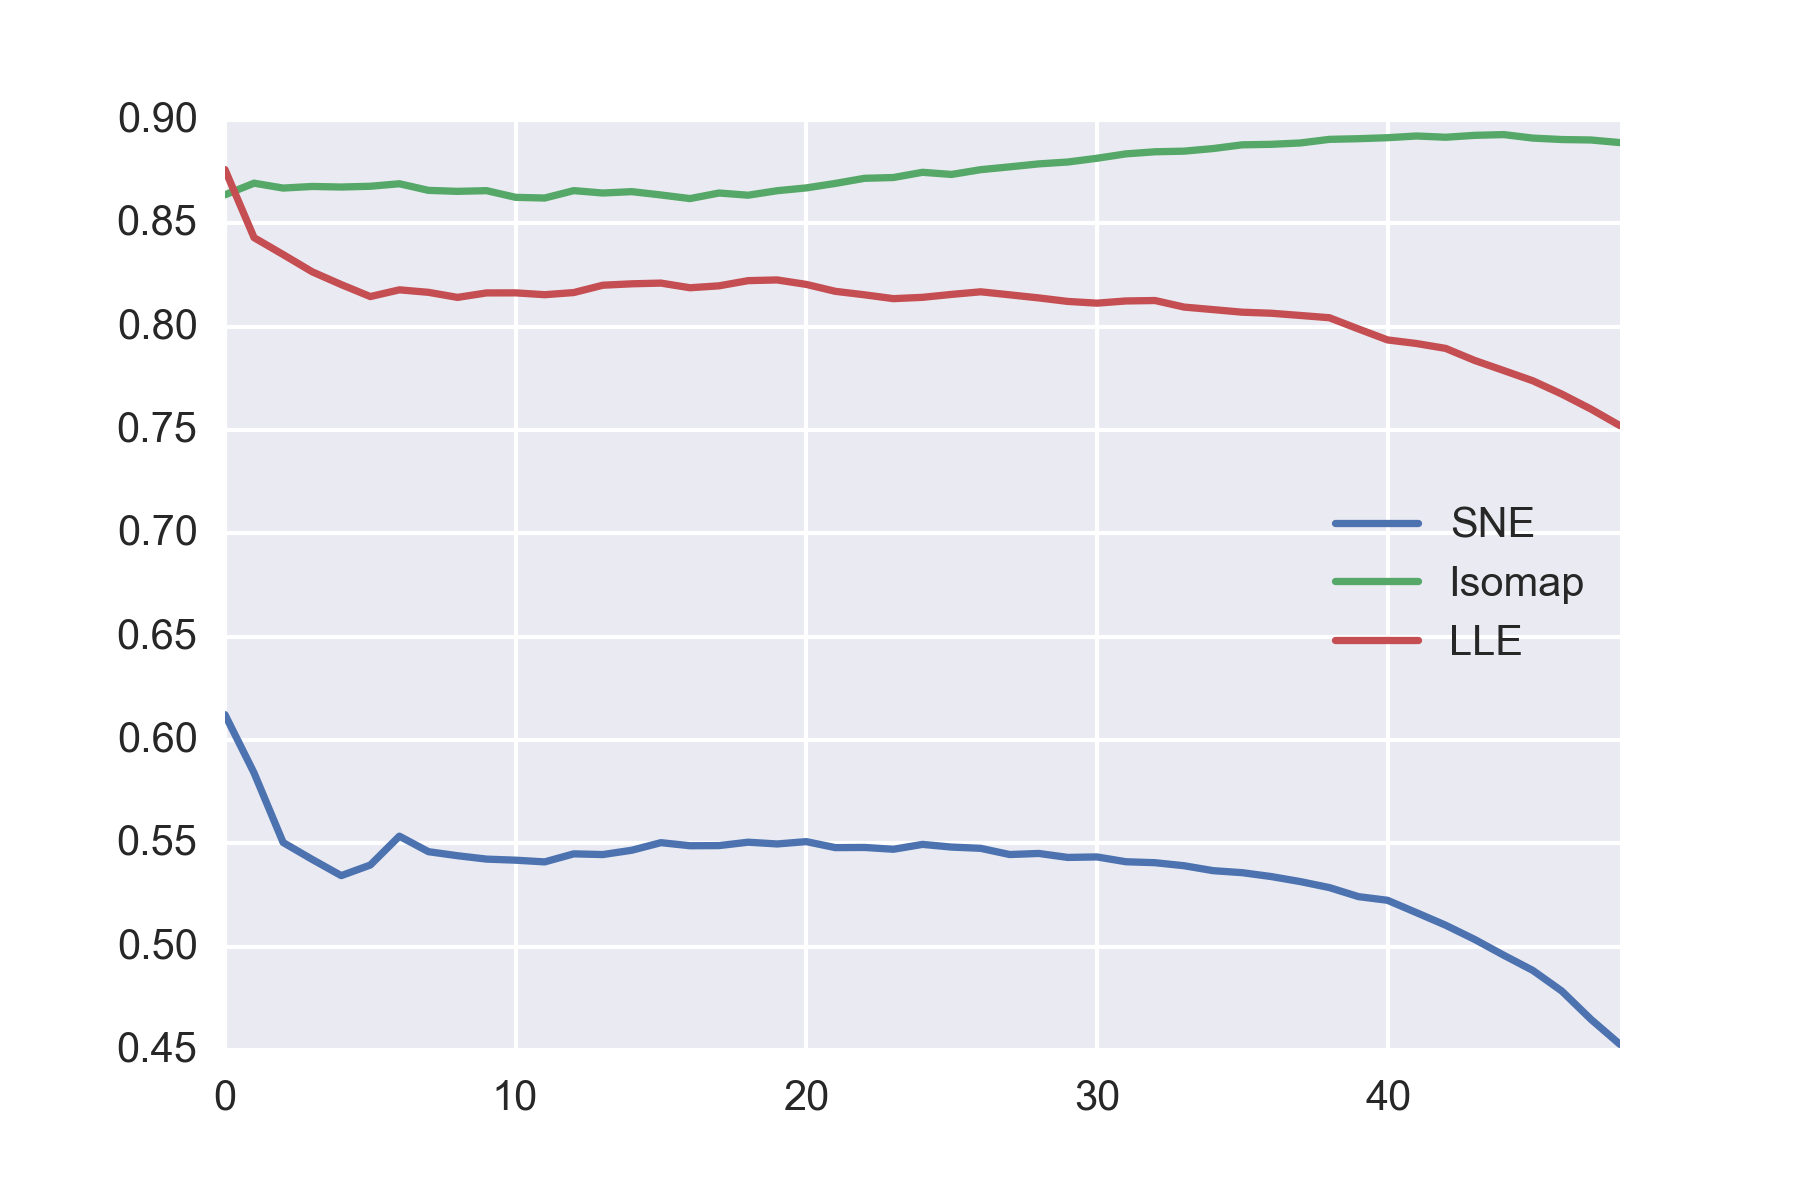
\includegraphics[width=0.49\textwidth]{figures/quality_measures/line_trustworthiness_3d.png}}
	\subfigure{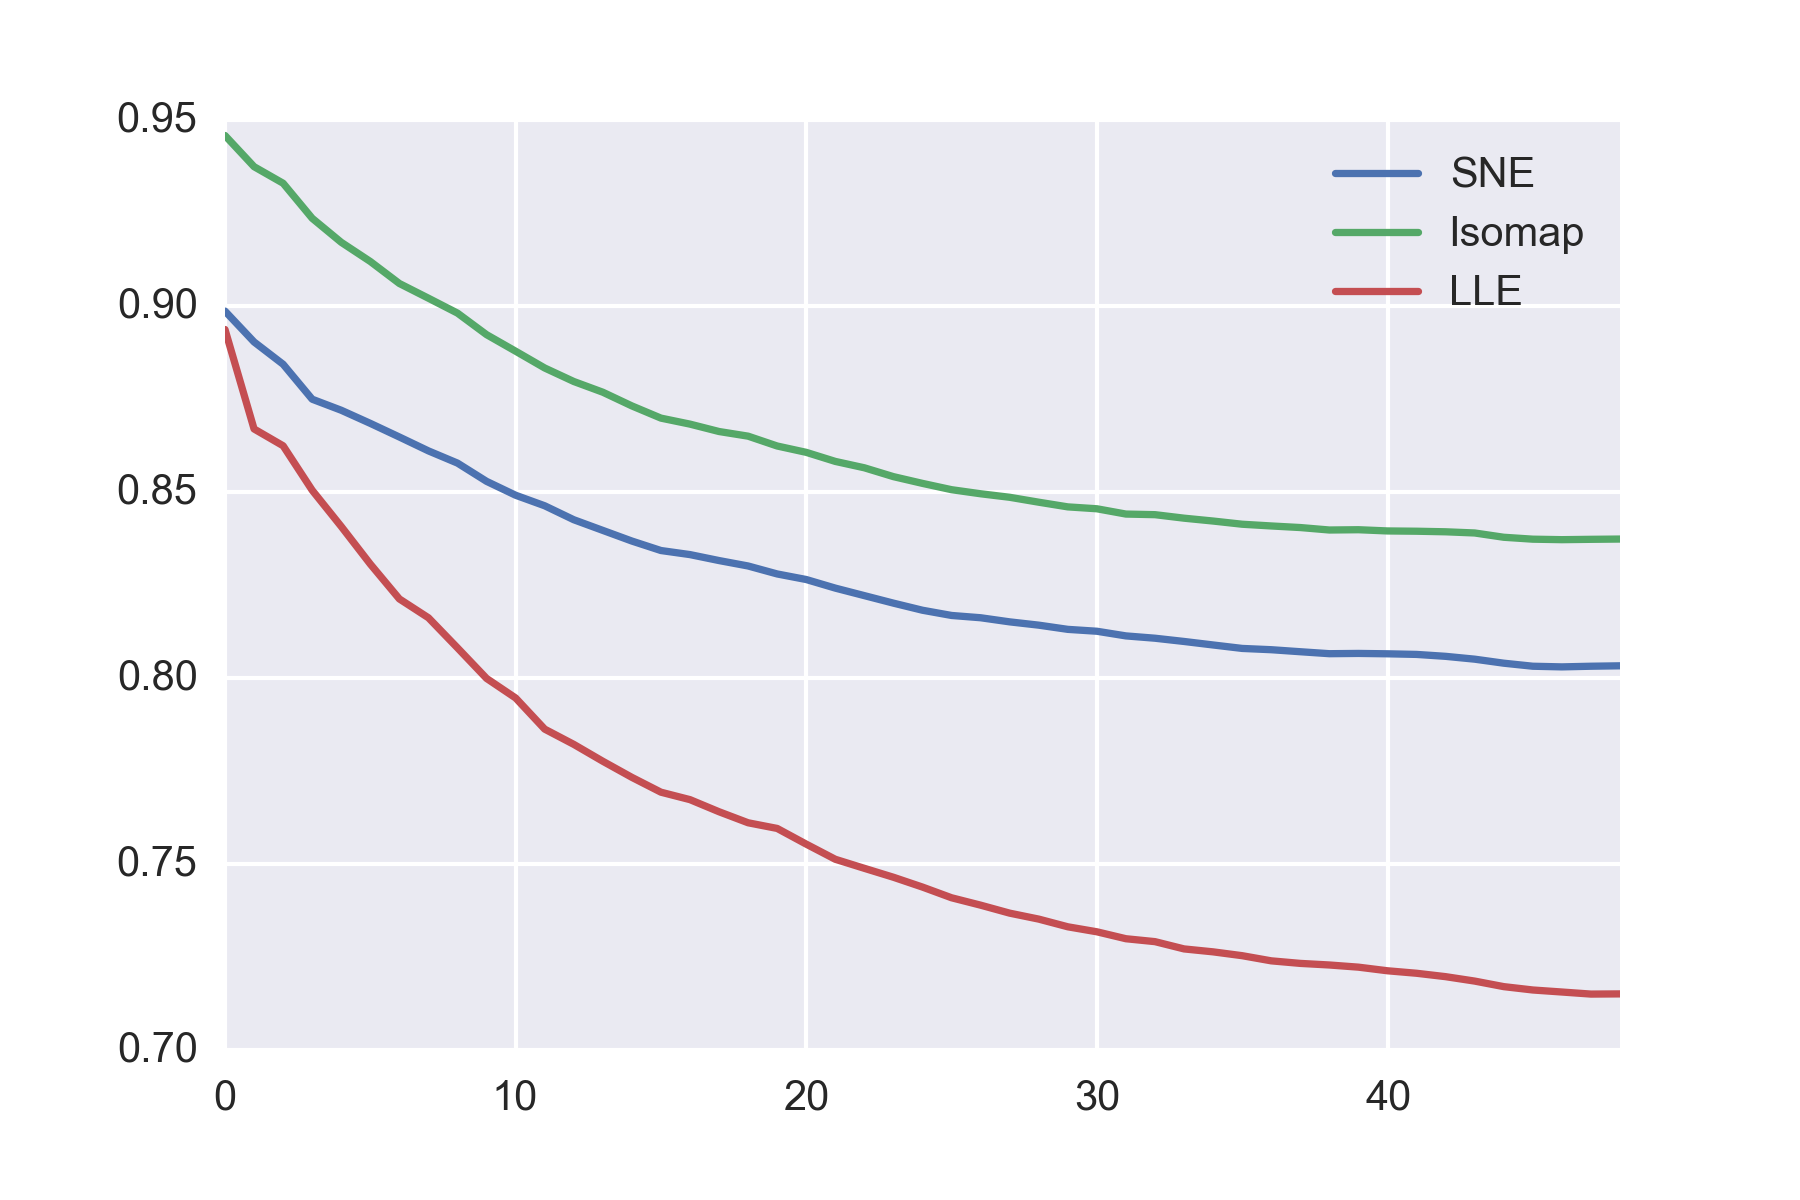
\includegraphics[width=0.49\textwidth]{figures/quality_measures/line_continuity_3d.png}}
	\caption{Trustworthiness (left) and continuity (right) of the 3D projections produced from line features.}\label{fig:TC_3d_lines}
\end{figure}

\begin{figure}[H]
	\centering
	\subfigure{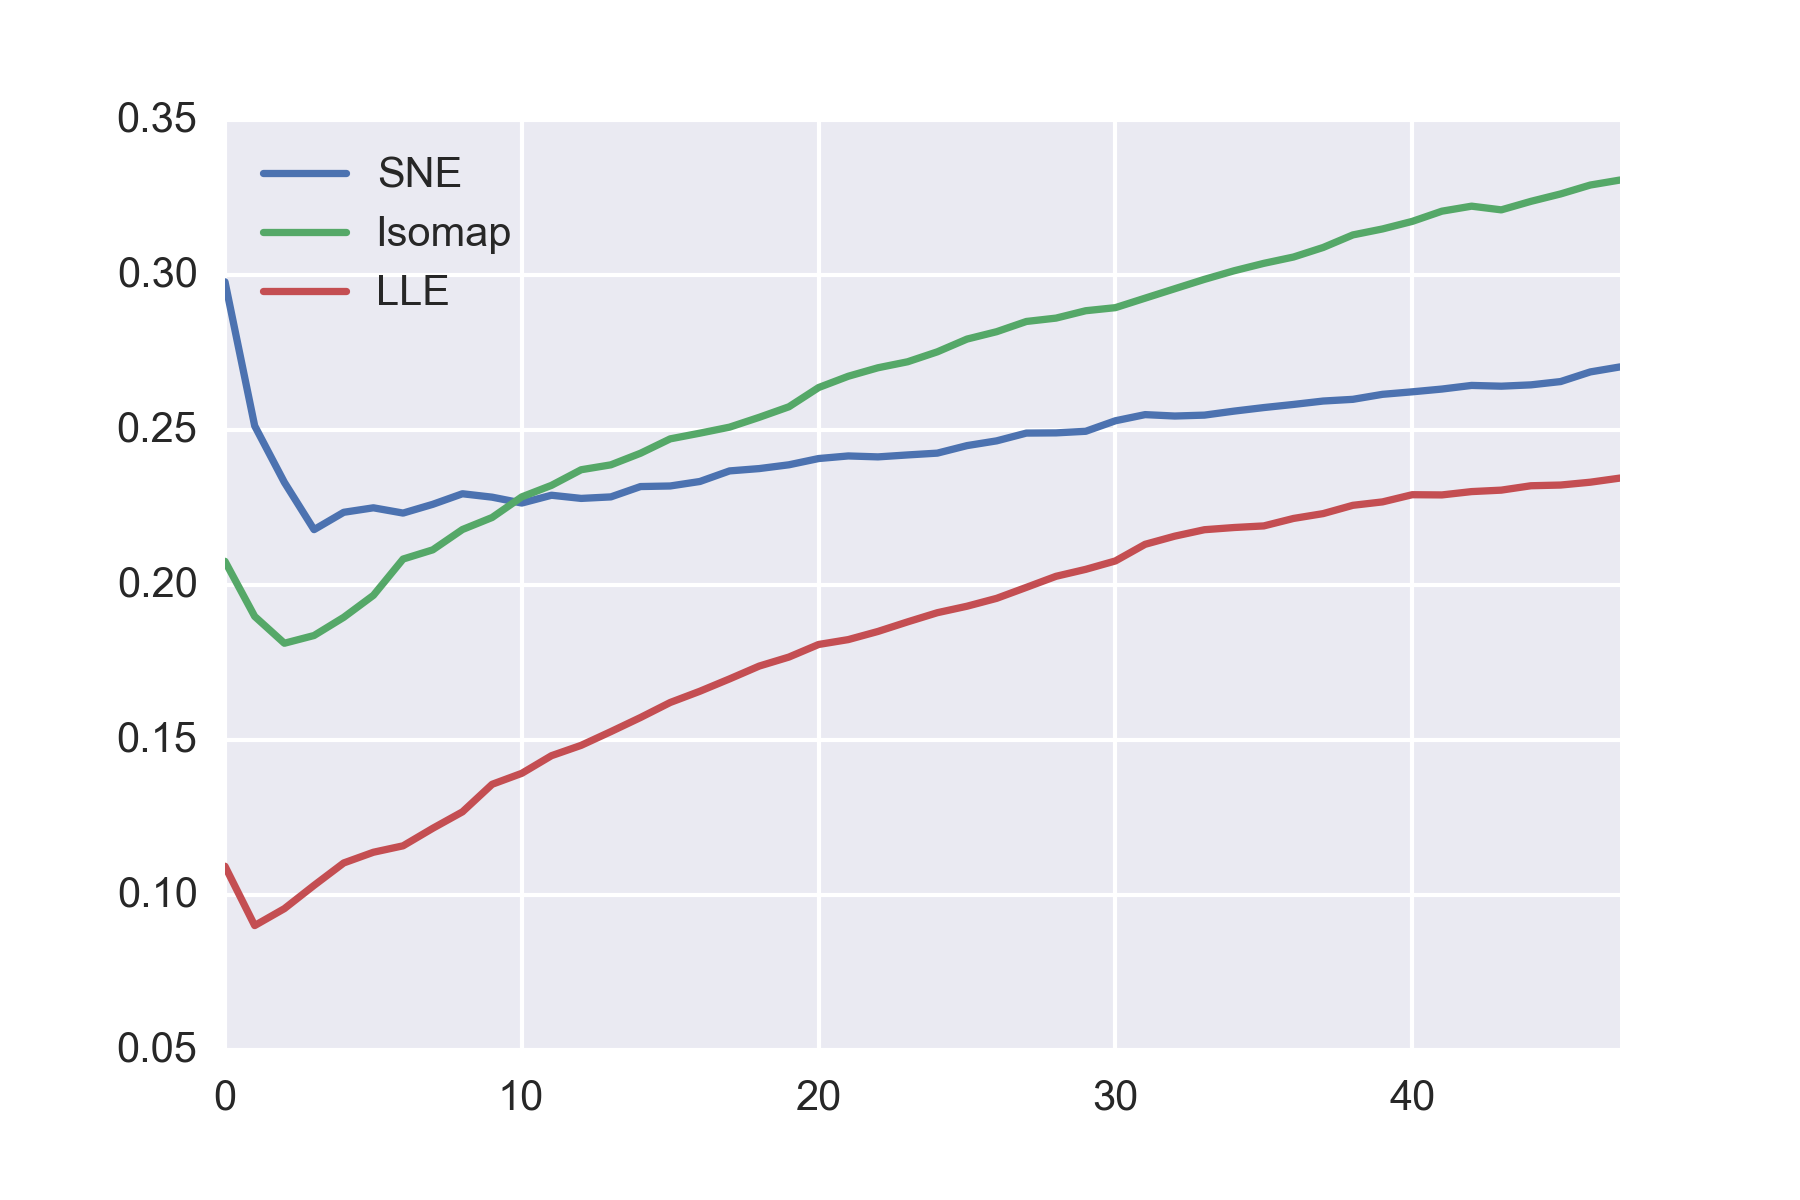
\includegraphics[width=0.49\textwidth]{figures/quality_measures/line_lcmc_2d.png}}
	\subfigure{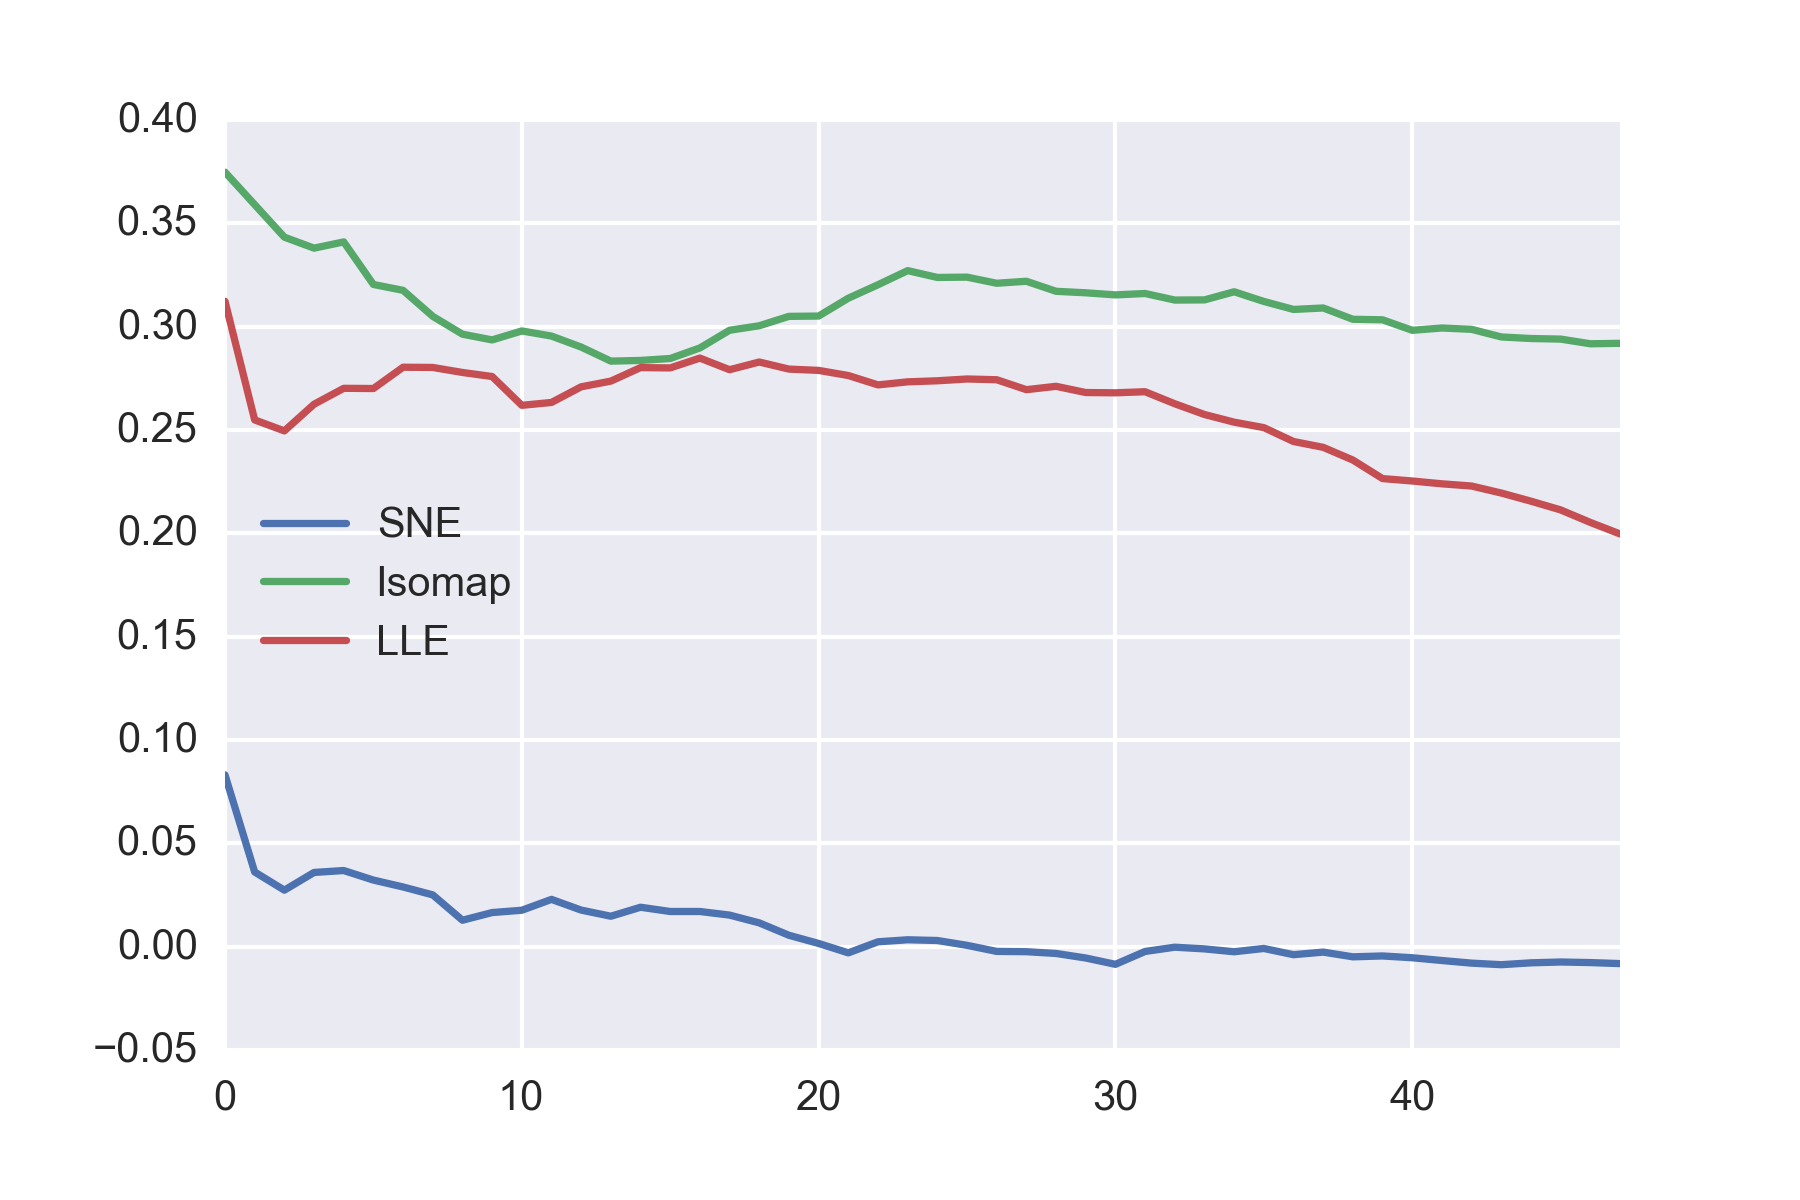
\includegraphics[width=0.49\textwidth]{figures/quality_measures/line_lcmc_3d.png}}
	\caption{LCMC of both the 2D projection (left) and 3D projection (right) of the feature space for lines.}\label{fig:LCMC_lines}
\end{figure}
\clearpage


\begin{figure}[H]
	\label{fig:mammogram-histogram}
	\centering
	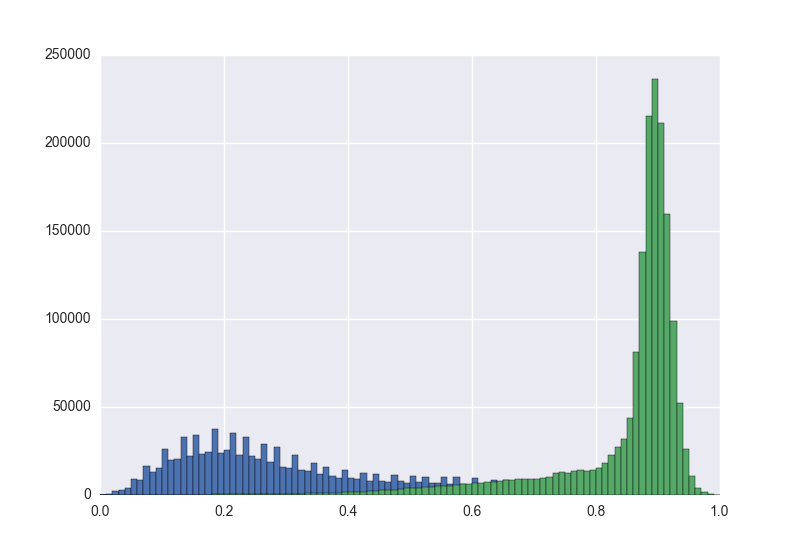
\includegraphics[width=0.8\textwidth]{Images/inverted_hist.png}	
	\caption{Comparison of the histogram of a real mammogram (blue) against a synthetic mammogram (green). The distribution of intensities are radically different from one another.}
\end{figure}

\subsection{Intensity \& Texture Features}
\label{subsec:results-texture}
Intensity and texture features showed the lowest similarity between the real and phantom datasets. As can be seen in figure \ref{fig:mammogram-histogram} the intensity distribution of the phantom mammograms are nothing like a real mammogram. Because of this difference the results show that the they are clearly in different spaces. The results of the KS two sample test showed that the two distributions generated for both intensity and texture features are completely different. The results of the two sample Kolmogorov-Smirnov test are included in appendix \ref{appendix:ks-test} because the number of features for blobs is based on the number of scales used leading to the a large number (up to 100) of entries. 

The feature spaces presented in this section were generated by taking ROIs defined by the blob and line features detected from each of the mammograms by computing intensity and texture features from each image patch. Because blobs are detected across a range of scales the average value for each scale is used leading to a feature space of size $nk$ where $n$ is the number of features and $k$ is the number of scales (e.g. for texture: $n = 4$ and $k = 10$ so it has $40$ features). 

The results of performing dimensionality reduction on both of these feature spaces is that in all almost all cases the synthetic mammograms are separated from the real mammograms into an isolated cluster on their own. This is because the values for both types of feature are on average much higher for the breast phantoms than the real mammograms.

For features derived from patches defined by blobs it can be seen that between the real mammograms there is a trend visible in both intensity and textural features which causes some transition between high to low risk. This is particularly visible for intensity features in the 2D plot produced by t-SNE shown in figure \ref{fig:intensity_SNE_mapping} and in the 2D plot for Isomap shown in figure \ref{fig:texture_iso_mapping} for texture features. For both intensity and texture feature LLE was shown to produce two clear clusters. One which contains the synthetics and one which contains the real mammograms. LLE still shows some variation between real in a similar way to what is seen in the projections produced by Isomap and LLE, but the resulting visualisation shows a much clear division.

In the case of intensity features this transition is caused by a higher detection of blobs which are of generally higher intensity. For texture features the trend is explained by a transition for blobs with low contrast and dissimilarity and high homogeneity and energy corresponding to high risk blobs transitioning through to low risk blobs where the reverse is true.

Intensity features derived from lines do show a degree of separation between high and low risk mammograms. High risk mammograms typically have a higher average intensity. This is most clearly seen in the 2D visualisation produced by t-SNE in \ref{fig:intensity_SNE_mapping_lines}. On the other hand the texture features do not appear to show any meaningful relationship between risk classes. LLE shows results that are also very similar to what is seen in blob features and the reasons behind this splitting are much the same.

The quality measures for intensity features derived from blobs show that these visualisations are generally less faithful in comparison to shape based features. Isomap is again a winner here with it producing better visualisations across all measures. Both t-SNE and LLE generally performed much worse than Isomap. The embedding by texture features are much more faithful. The 2D projections show a close call between Isomap and t-SNE. For 3D projections t-SNE is the clear loser, being dramatically worse compared with t-SNE and Isomap.

Quality measures taken from the visualisations for intensity from lines show that the mapping produced by Isomap is better for projections in both two and three dimensions, but that t-SNE is at least comparable to Isomap in 2D. The results for texture features derived from lines show that the t-SNE performance of t-SNE is better for 2D. In the three dimensions Isomap is again a clear winner.

%------------------------------------------------------------------------------------
% Blob intensity and texture features
%------------------------------------------------------------------------------------


\clearpage
\begin{figure}[H]
	\centering
	\subfigure{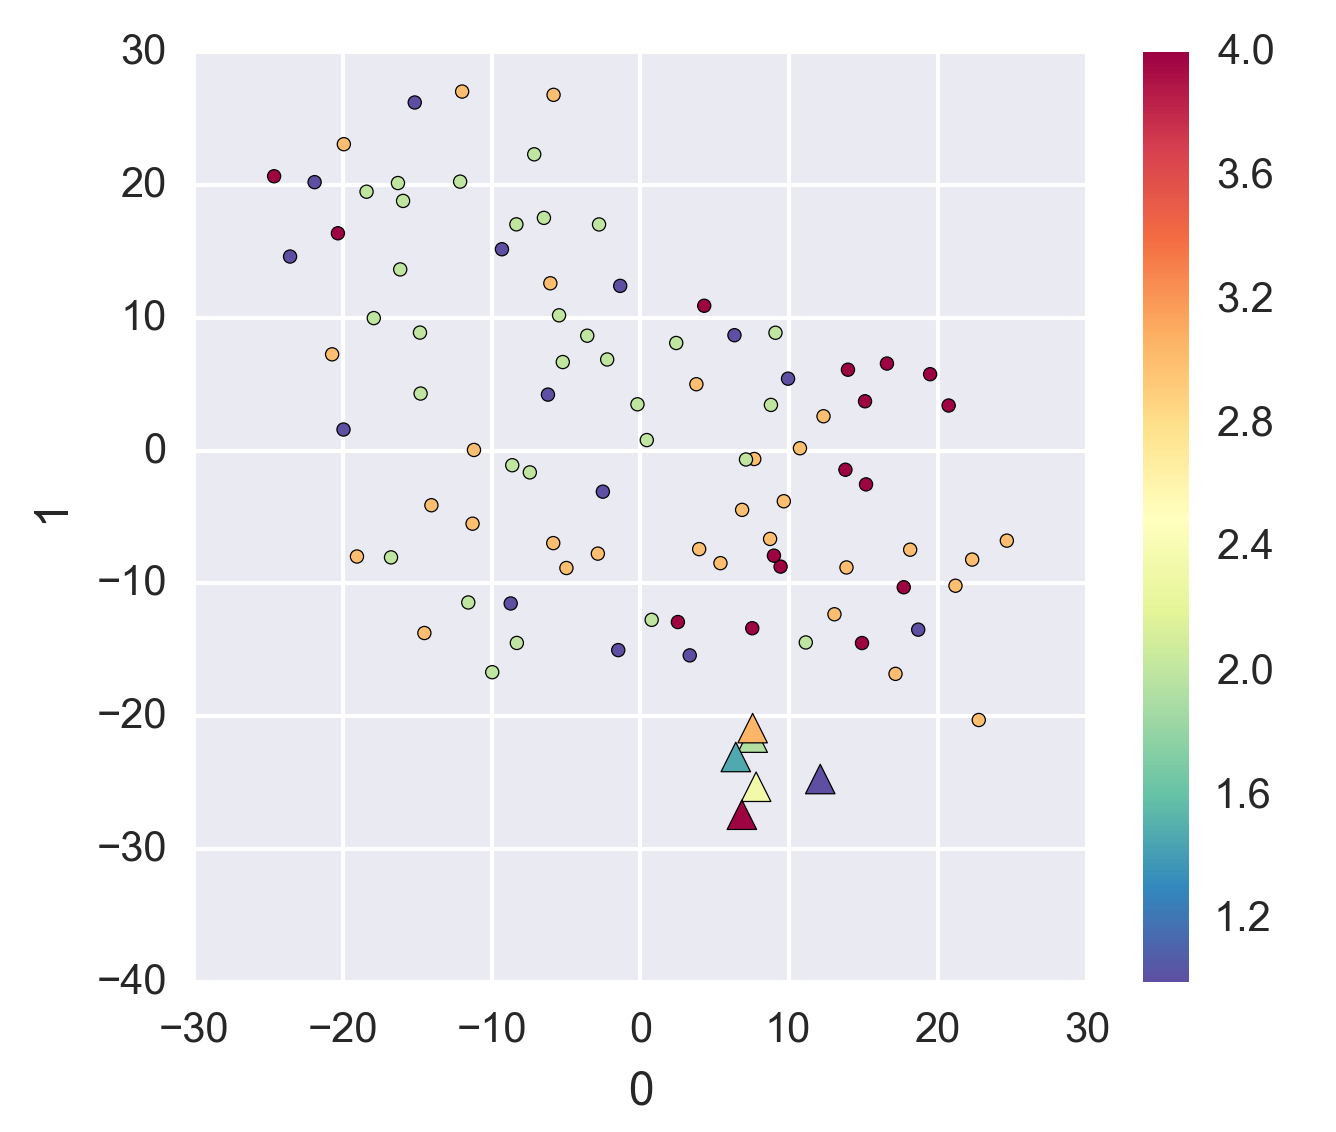
\includegraphics[width=0.4\textwidth]{figures/mappings/intensity_SNE_mapping_2d.png}}
	\subfigure{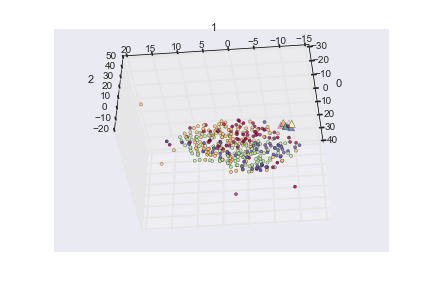
\includegraphics[width=0.49\textwidth]{figures/mappings/intensity_SNE_mapping_3d.png}}
	\caption{2D \& 3D projections of the intensity feature space produced by the t-SNE algorithm with a learning rate of 200 and perplexity of 20.}\label{fig:intensity_SNE_mapping}
\end{figure}

\begin{figure}[H]
	\centering
	\subfigure{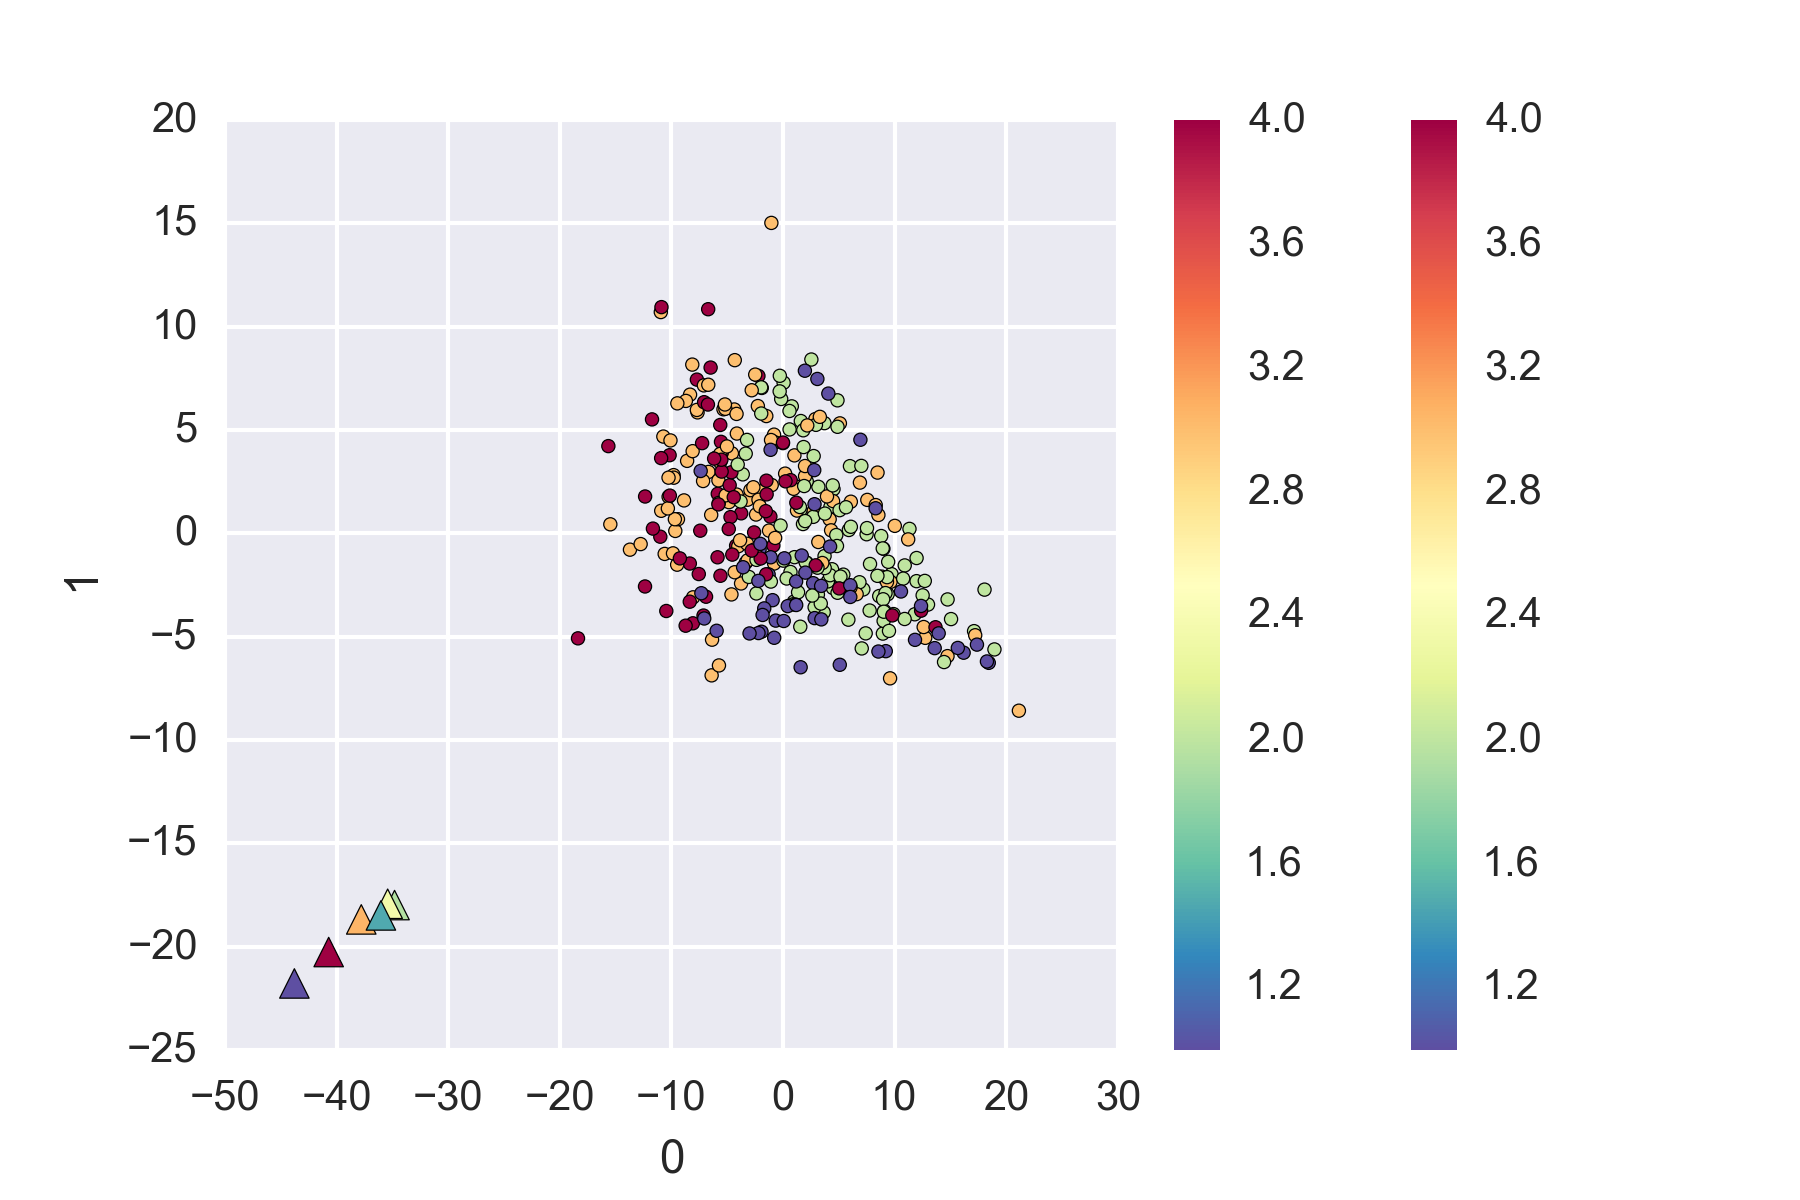
\includegraphics[width=0.4\textwidth]{figures/mappings/intensity_iso_mapping_2d.png}}
	\subfigure{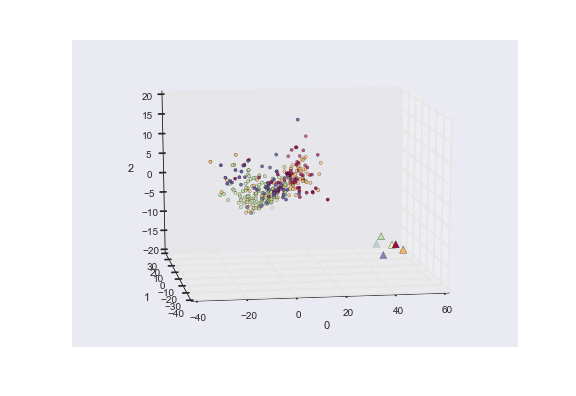
\includegraphics[width=0.49\textwidth]{figures/mappings/intensity_iso_mapping_3d.png}}
	\caption{2D \& 3D projections of the intensity feature space generated from blobs produced by the Isomap algorithm with 4 neighbours.}\label{fig:intensity_iso_mapping}
\end{figure}

\begin{figure}[H]
	\centering
	\subfigure{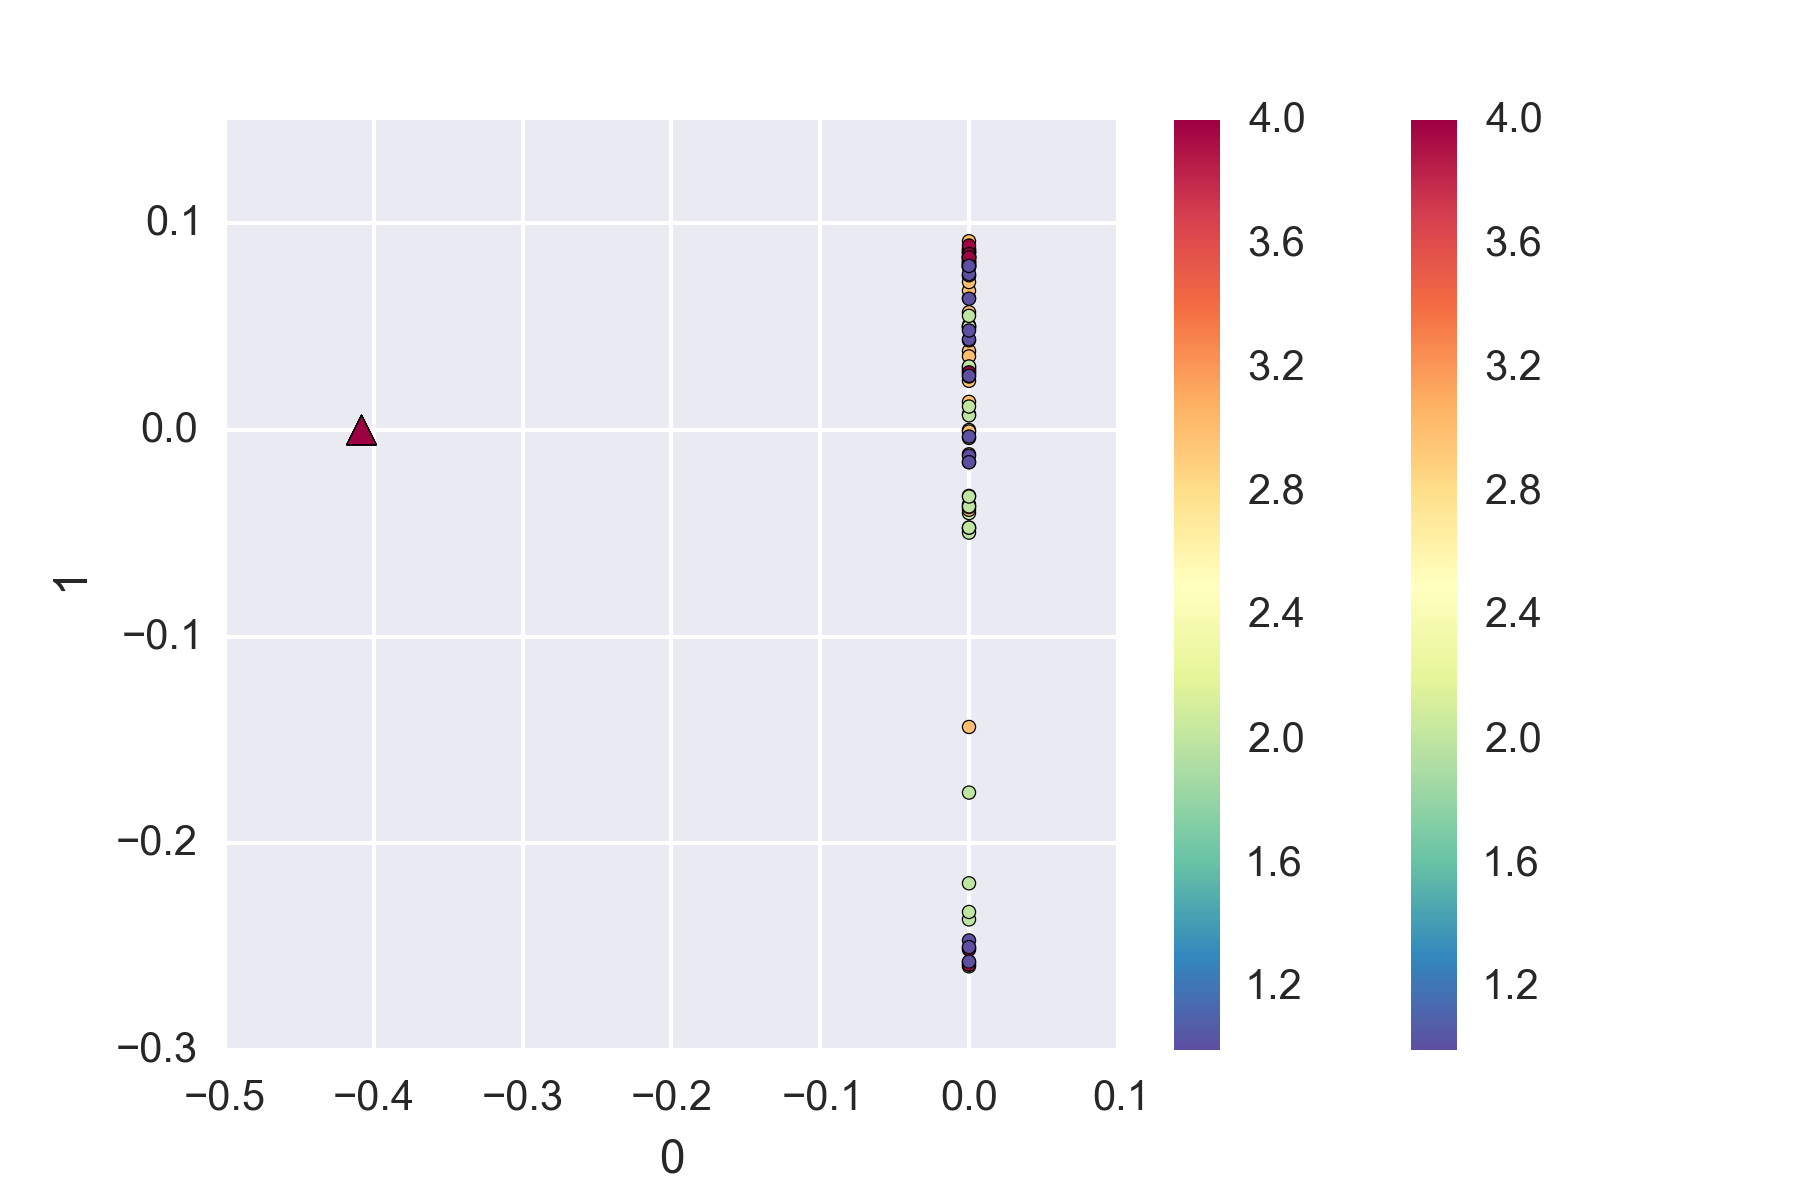
\includegraphics[width=0.4\textwidth]{figures/mappings/intensity_lle_mapping_2d.png}}
	\subfigure{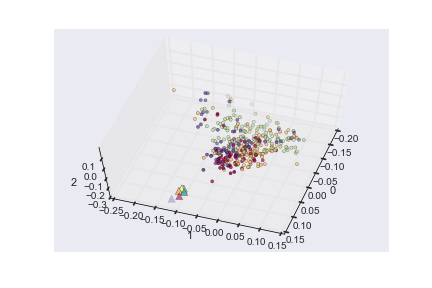
\includegraphics[width=0.49\textwidth]{figures/mappings/intensity_lle_mapping_3d.png}}
	\caption{2D \& 3D projections of the intensity feature space generated from blobs produced by the LLE algorithm with 4 neighbours.}\label{fig:intensity_LLE_mapping}
\end{figure}
\clearpage

% Quality for blob intensity features
%------------------------------------------------------------------------------------
\clearpage
\begin{figure}[H]
	\centering
	\subfigure{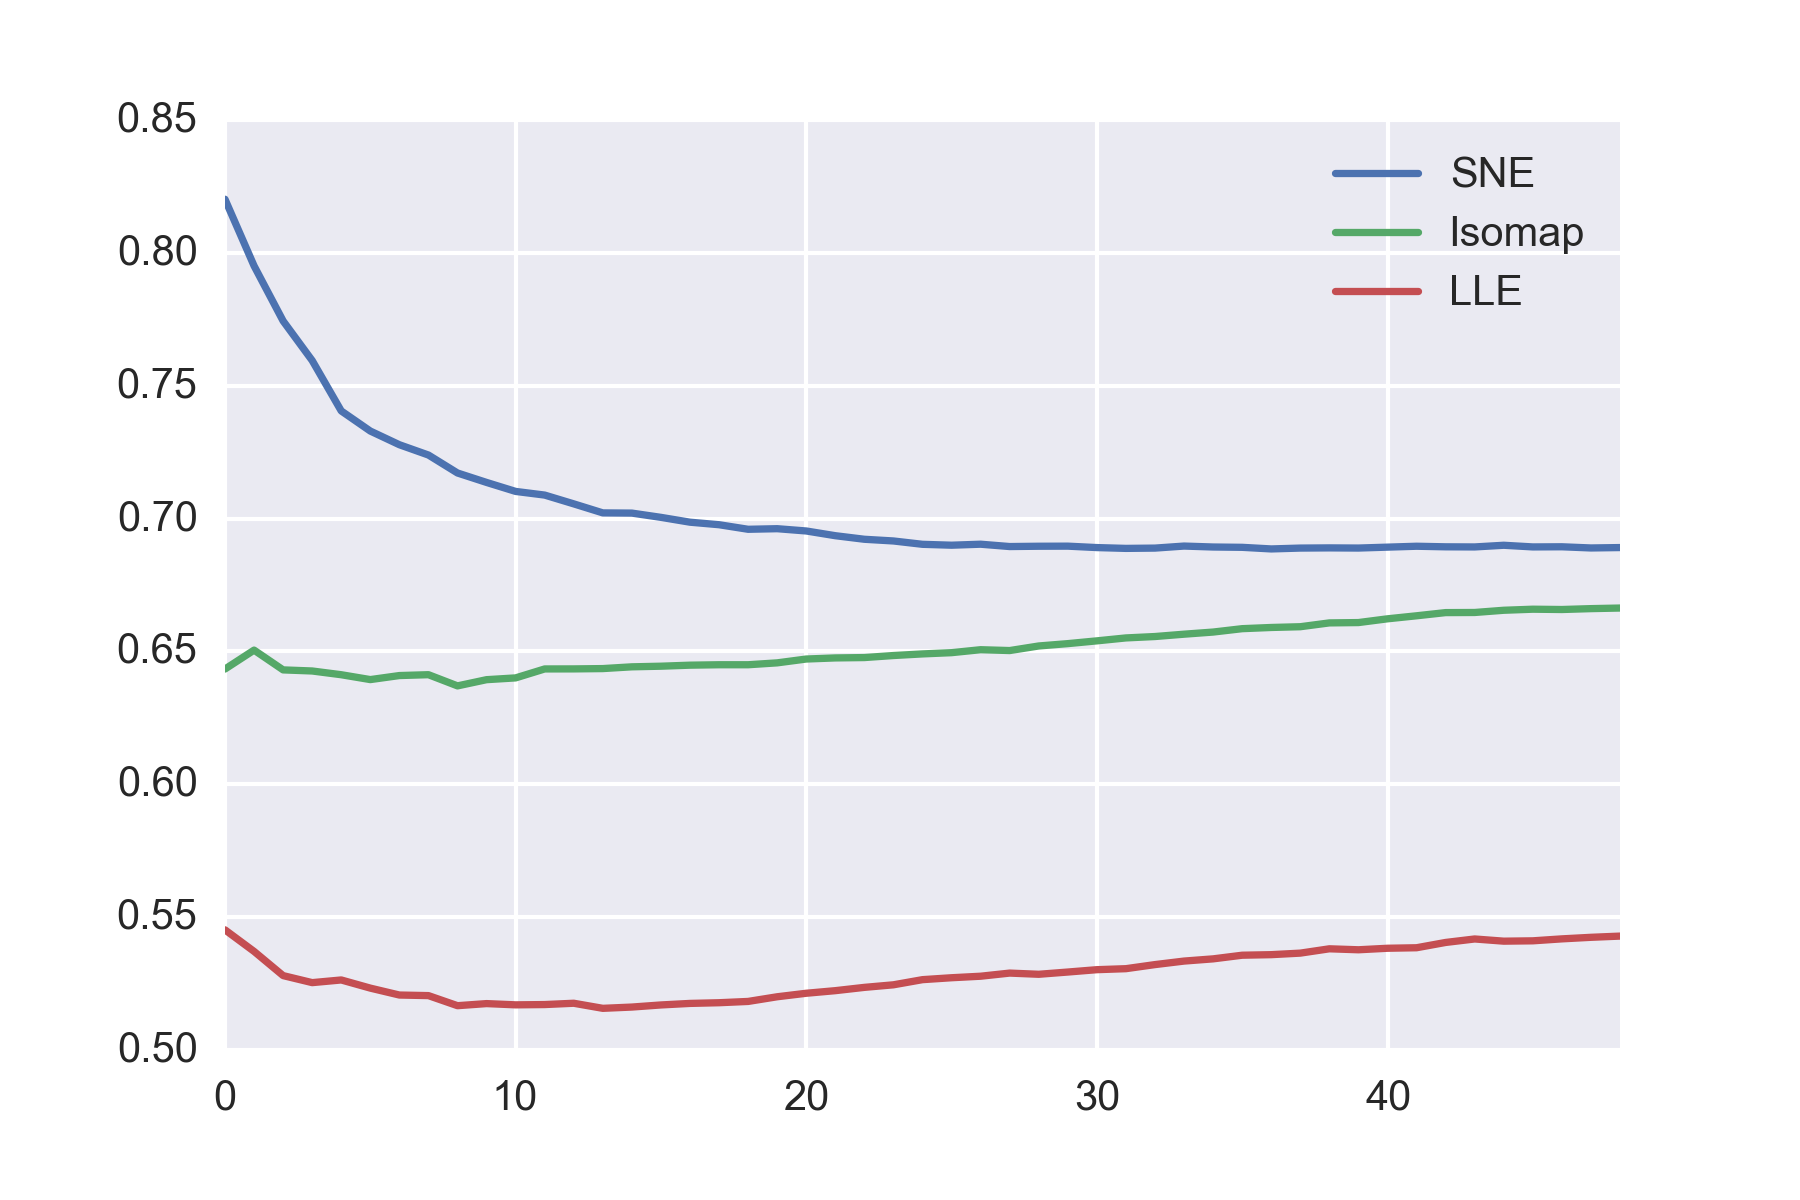
\includegraphics[width=0.49\textwidth]{figures/quality_measures/intensity_trustworthiness_2d.png}}
	\subfigure{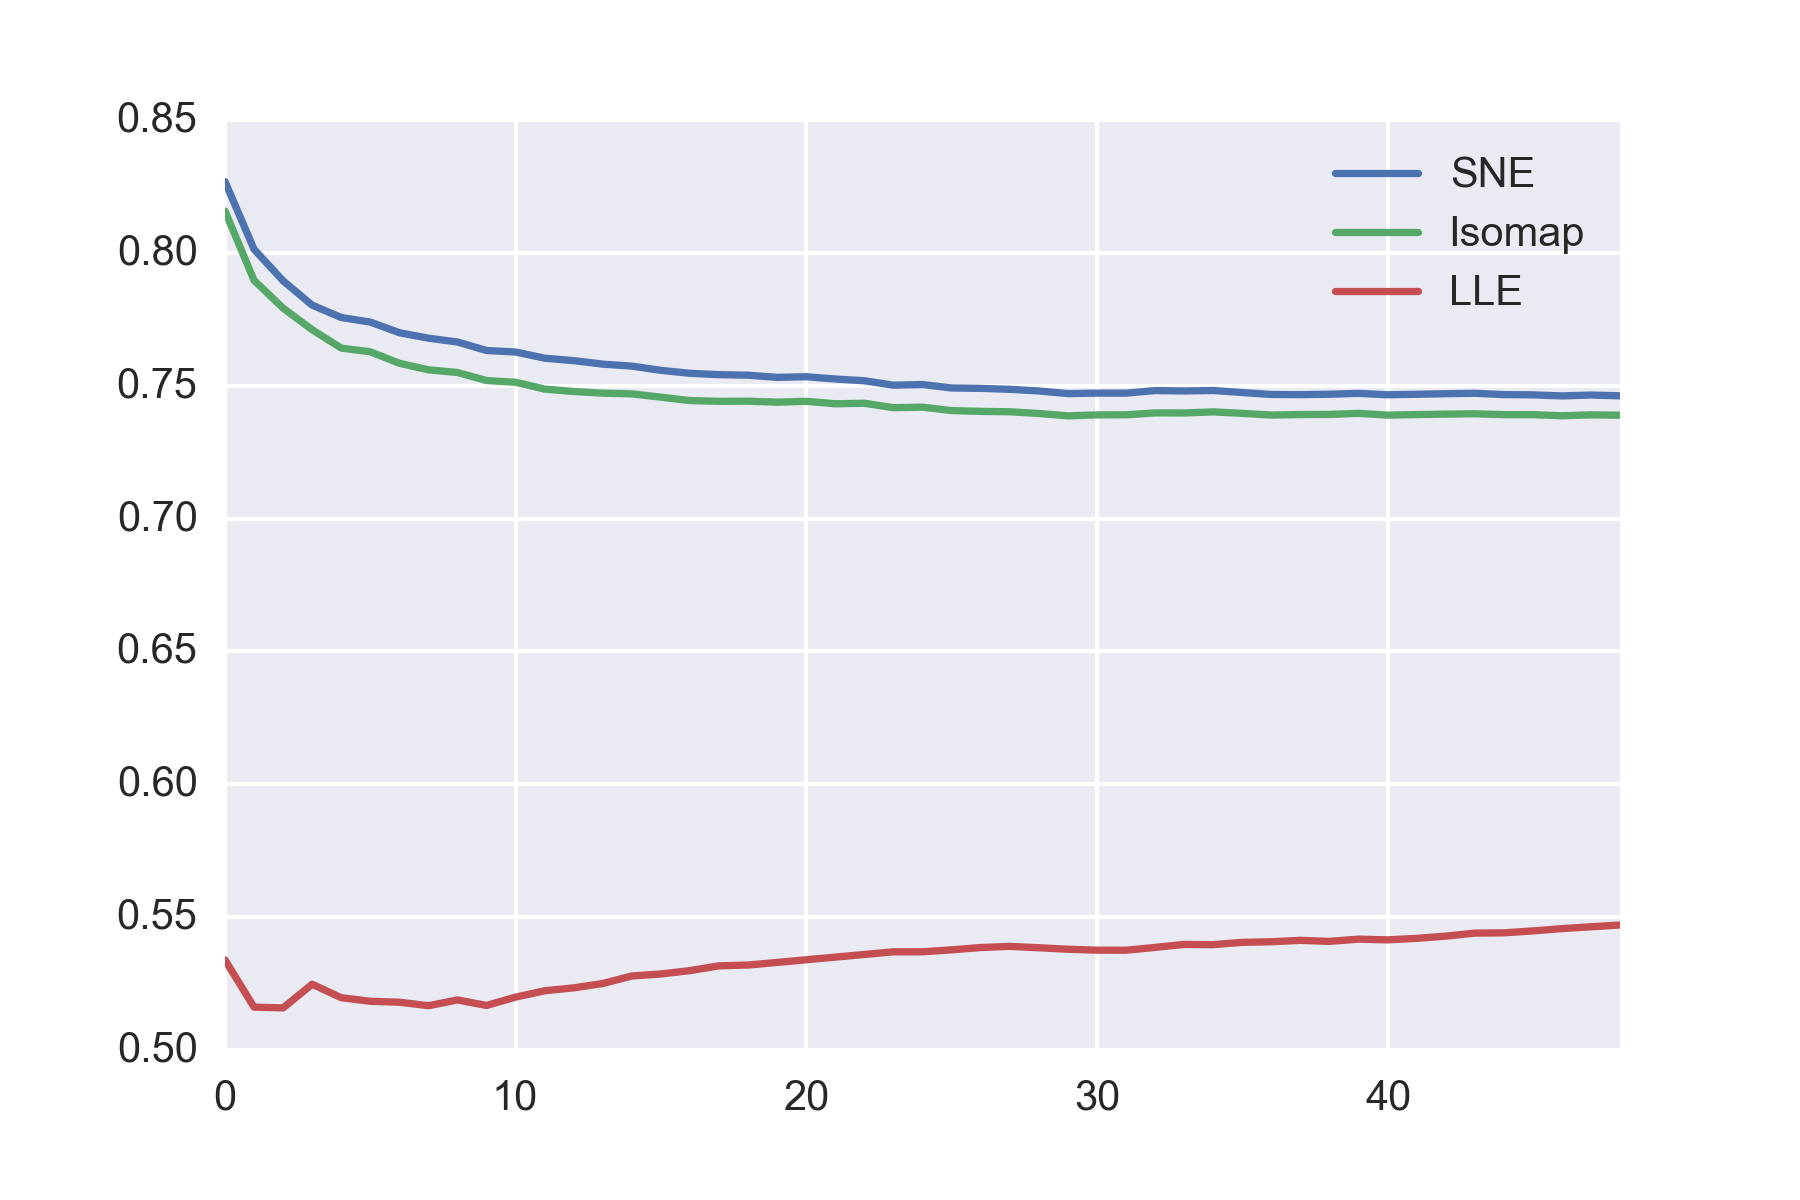
\includegraphics[width=0.49\textwidth]{figures/quality_measures/intensity_continuity_2d.png}}
	\caption{Trustworthiness (left) and continuity (right) of the 2D projections produced from intensity features from blobs.}\label{fig:TC_2d_intensity}
\end{figure}

\begin{figure}[H]
	\centering
	\subfigure{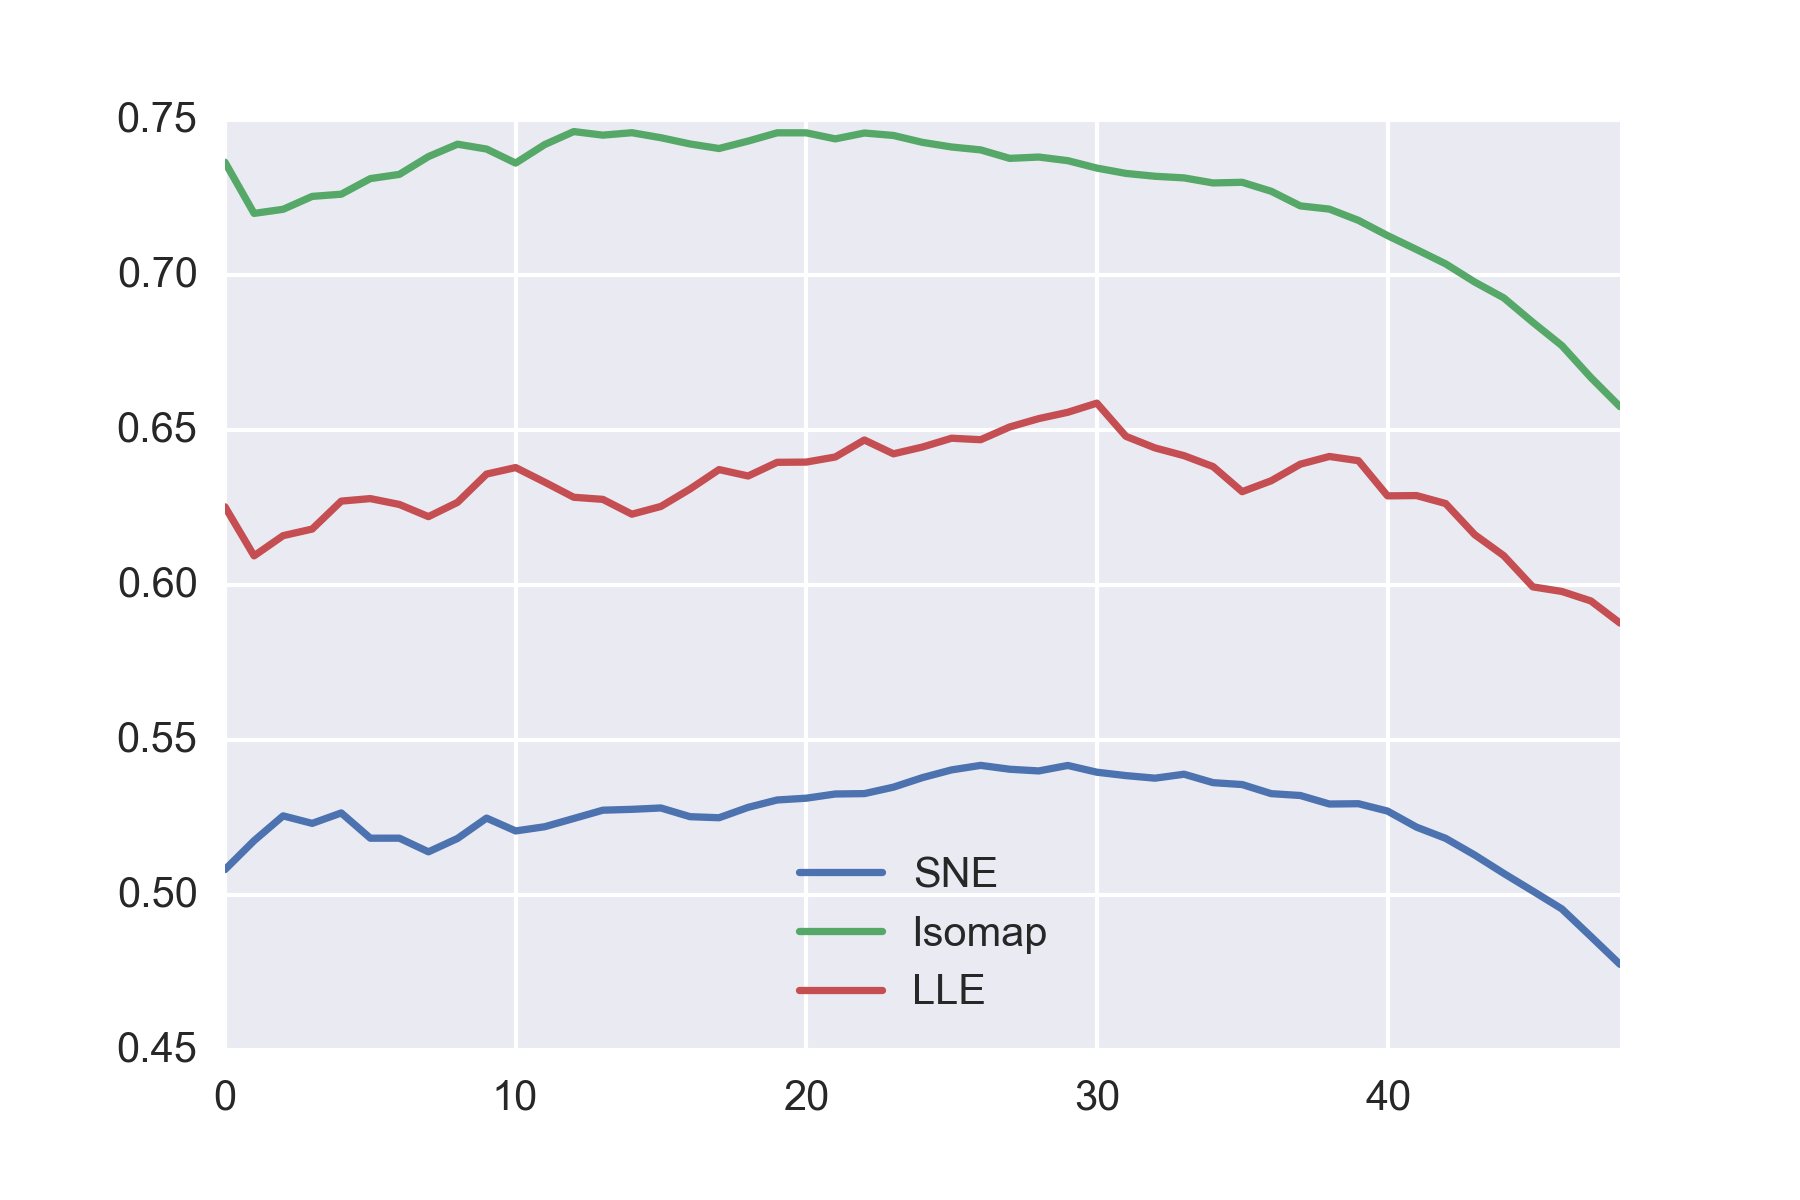
\includegraphics[width=0.49\textwidth]{figures/quality_measures/intensity_trustworthiness_3d.png}}
	\subfigure{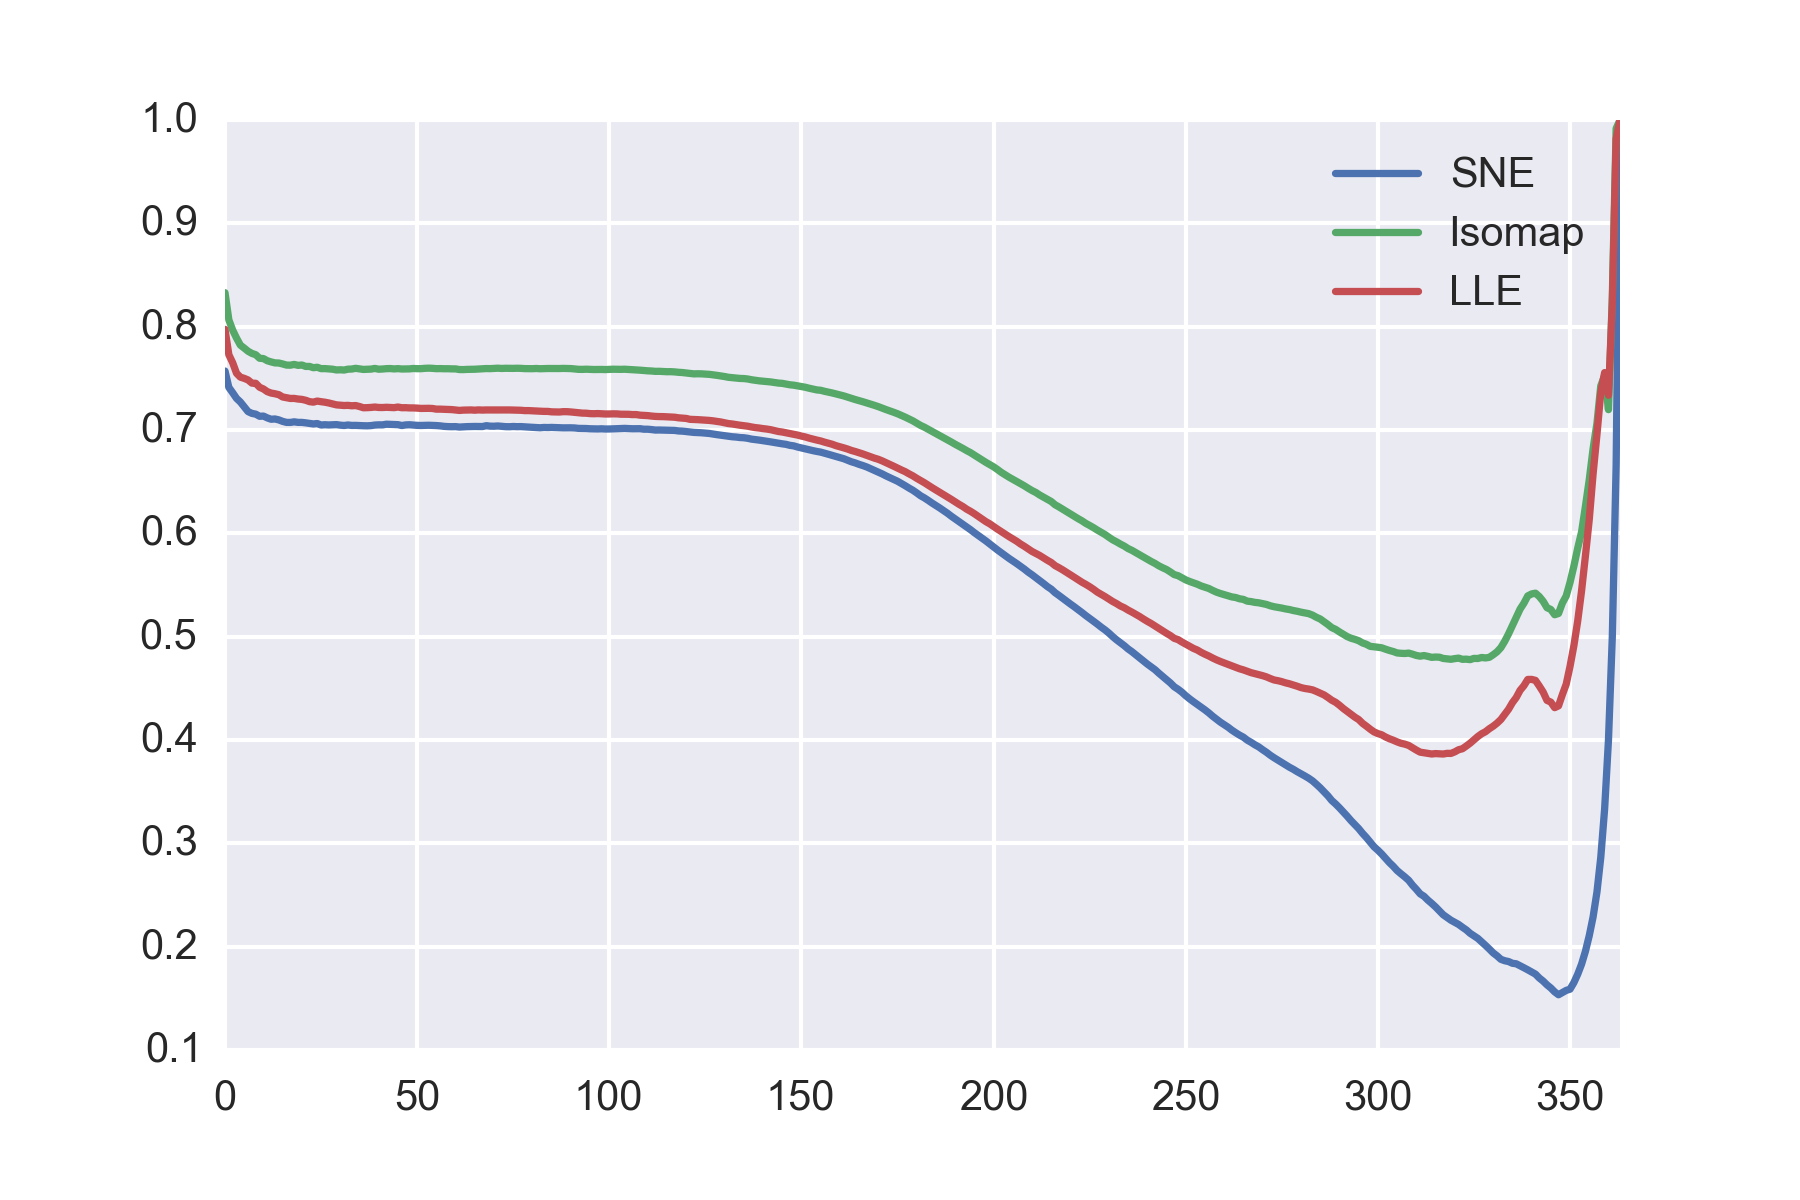
\includegraphics[width=0.49\textwidth]{figures/quality_measures/intensity_continuity_3d.png}}
	\caption{Trustworthiness (left) and continuity (right) of the 3D projections produced from intensity features from blobs.}\label{fig:TC_3d_intensity}
\end{figure}

\begin{figure}[H]
	\centering
	\subfigure{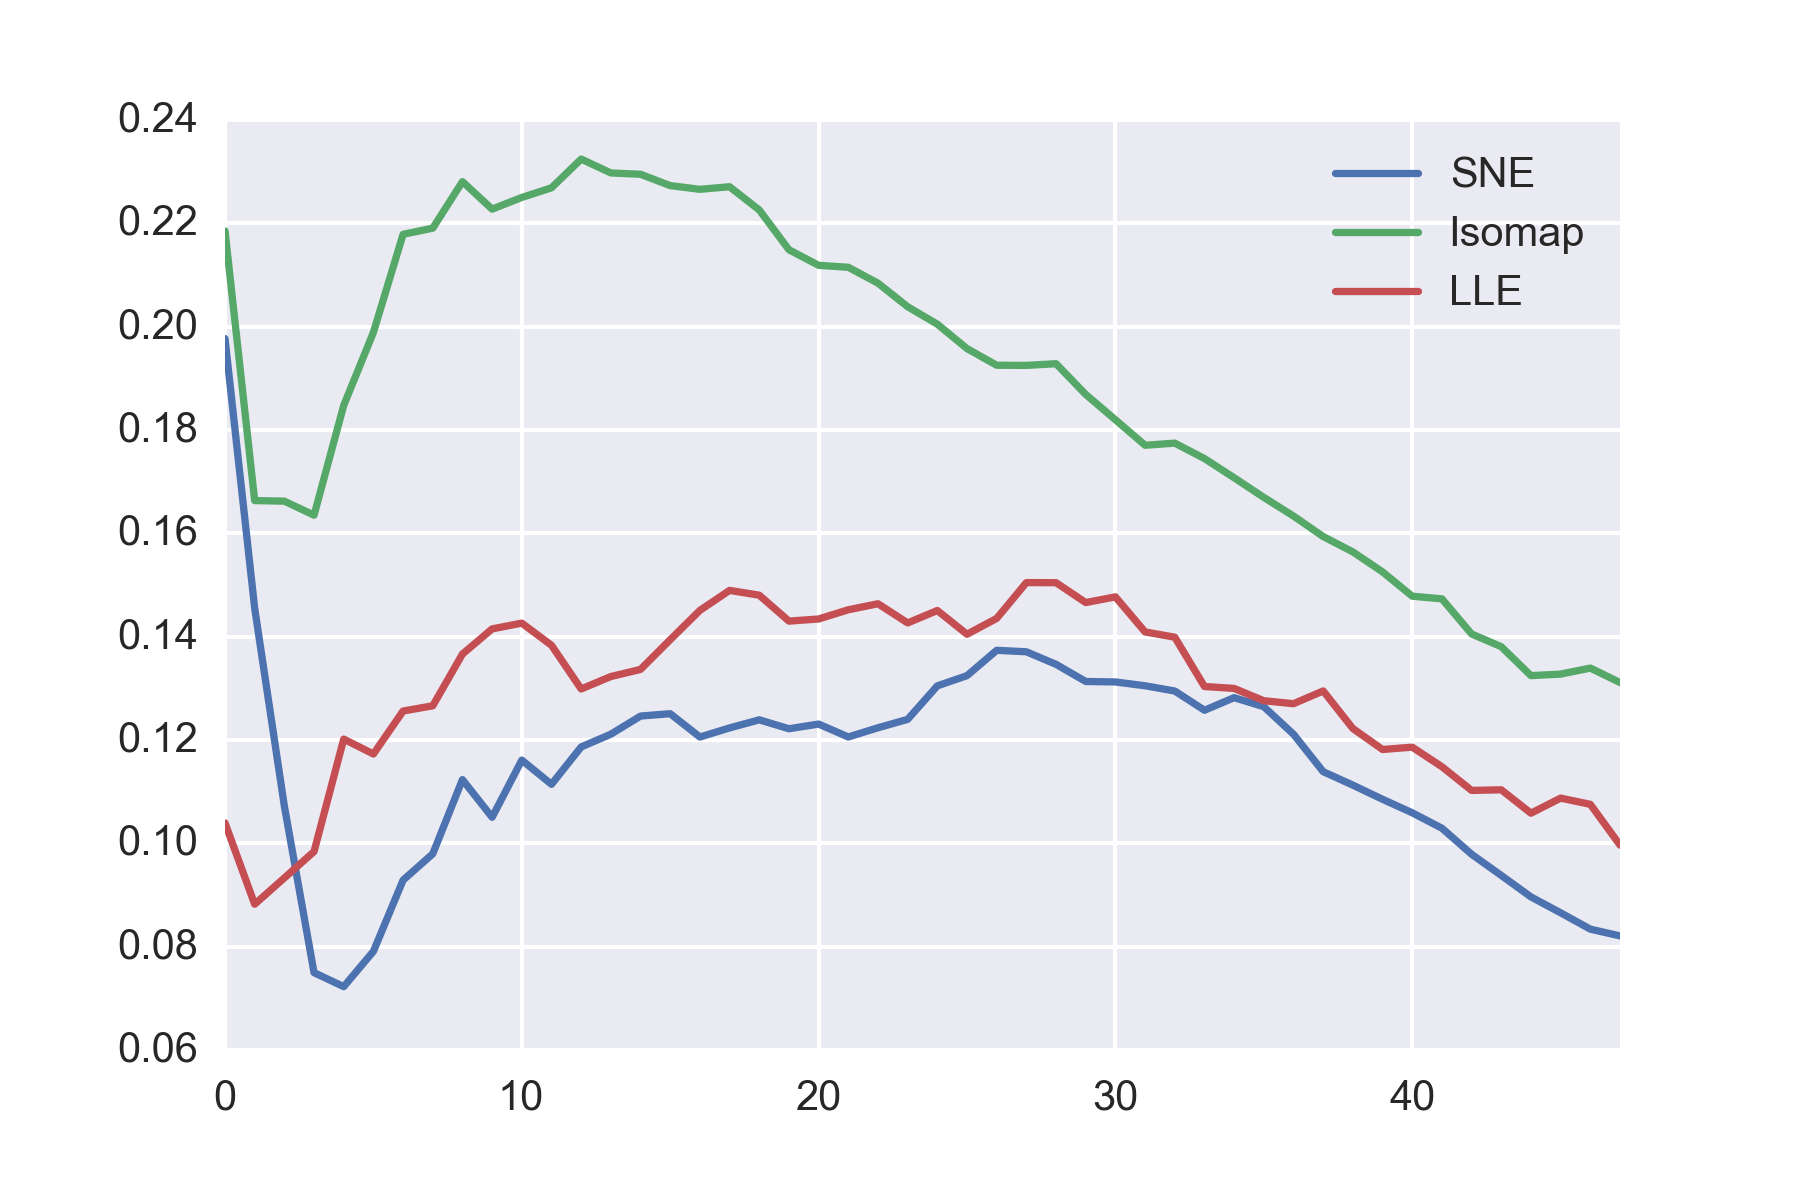
\includegraphics[width=0.49\textwidth]{figures/quality_measures/intensity_lcmc_2d.png}}
	\subfigure{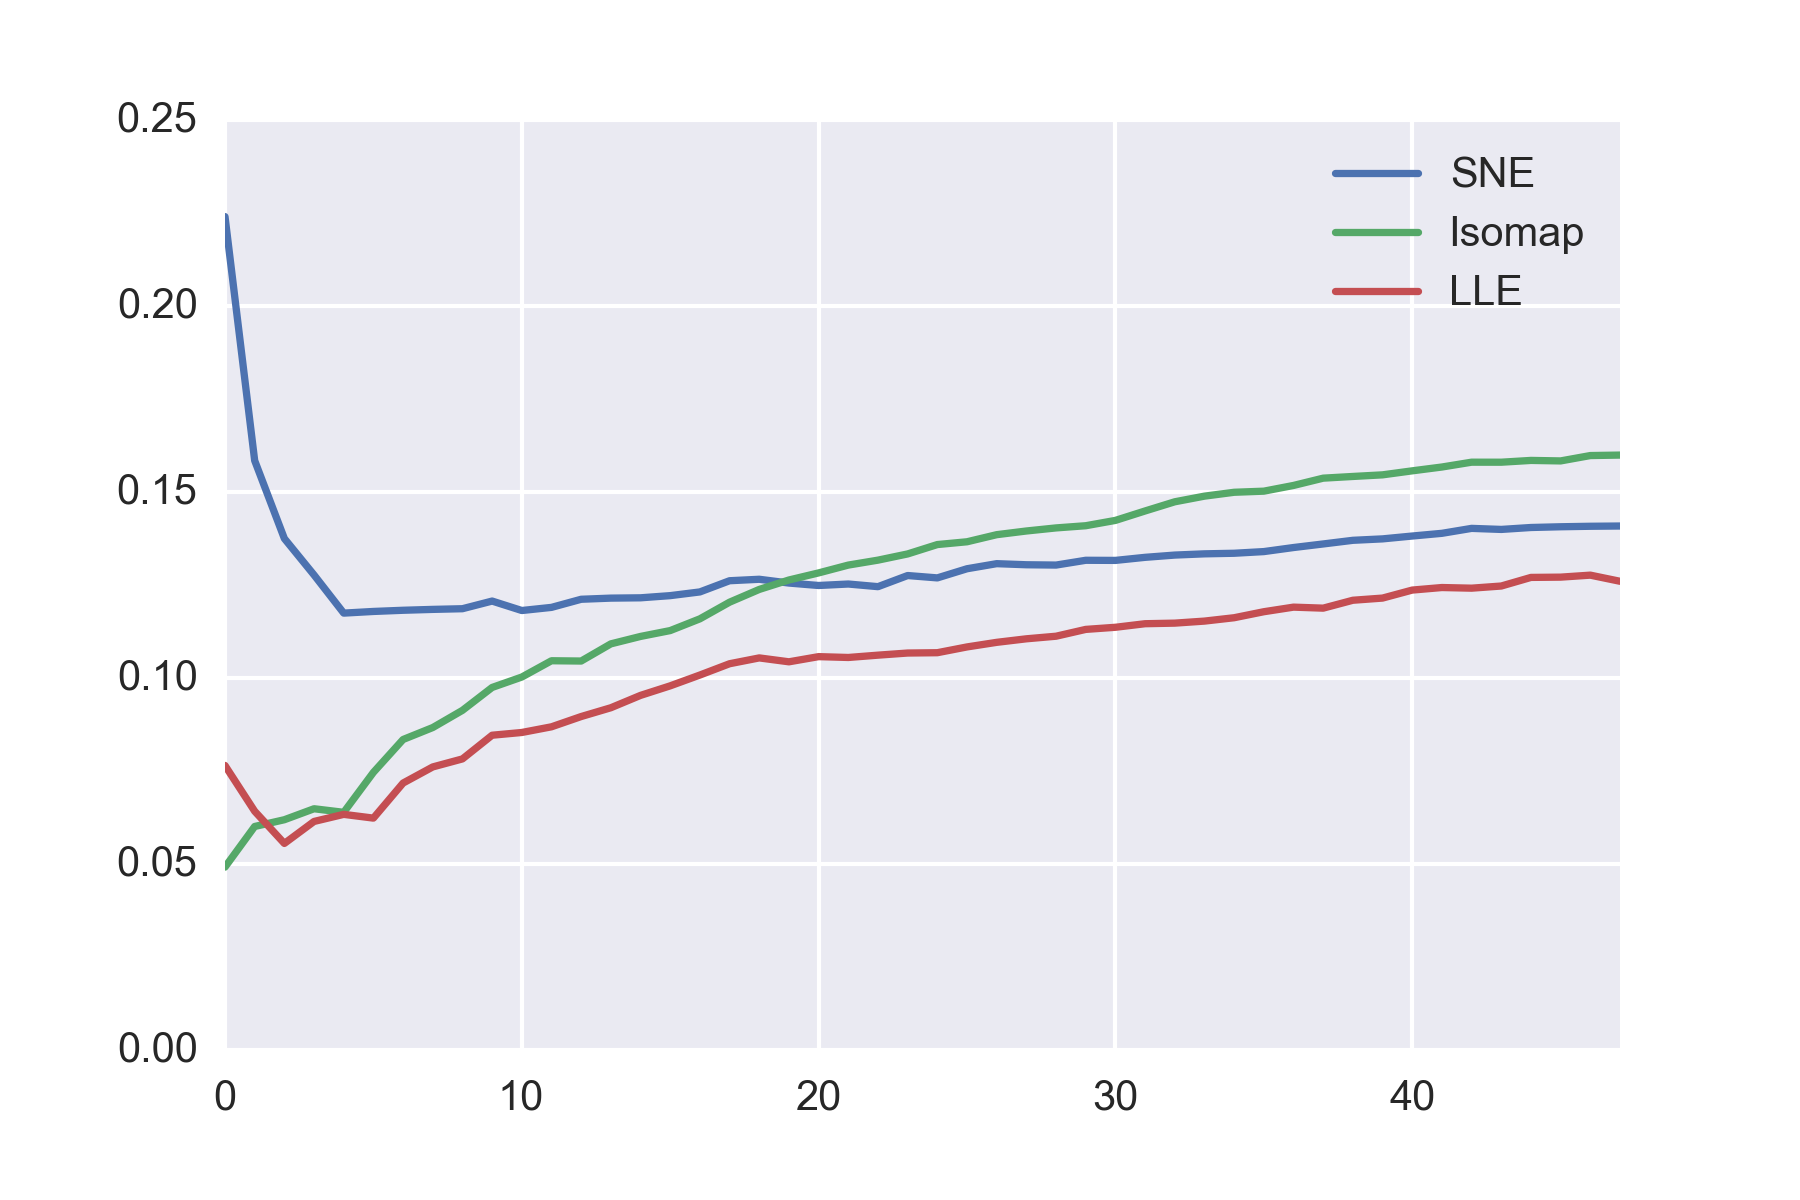
\includegraphics[width=0.49\textwidth]{figures/quality_measures/intensity_lcmc_3d.png}}
	\caption{LCMC of both the 2D projection (left) and 3D projection (right) of the feature space for intensity from blobs.}\label{fig:LCMC_intensity}
\end{figure}
\clearpage

\clearpage
\begin{figure}[H]
	\centering
	\subfigure{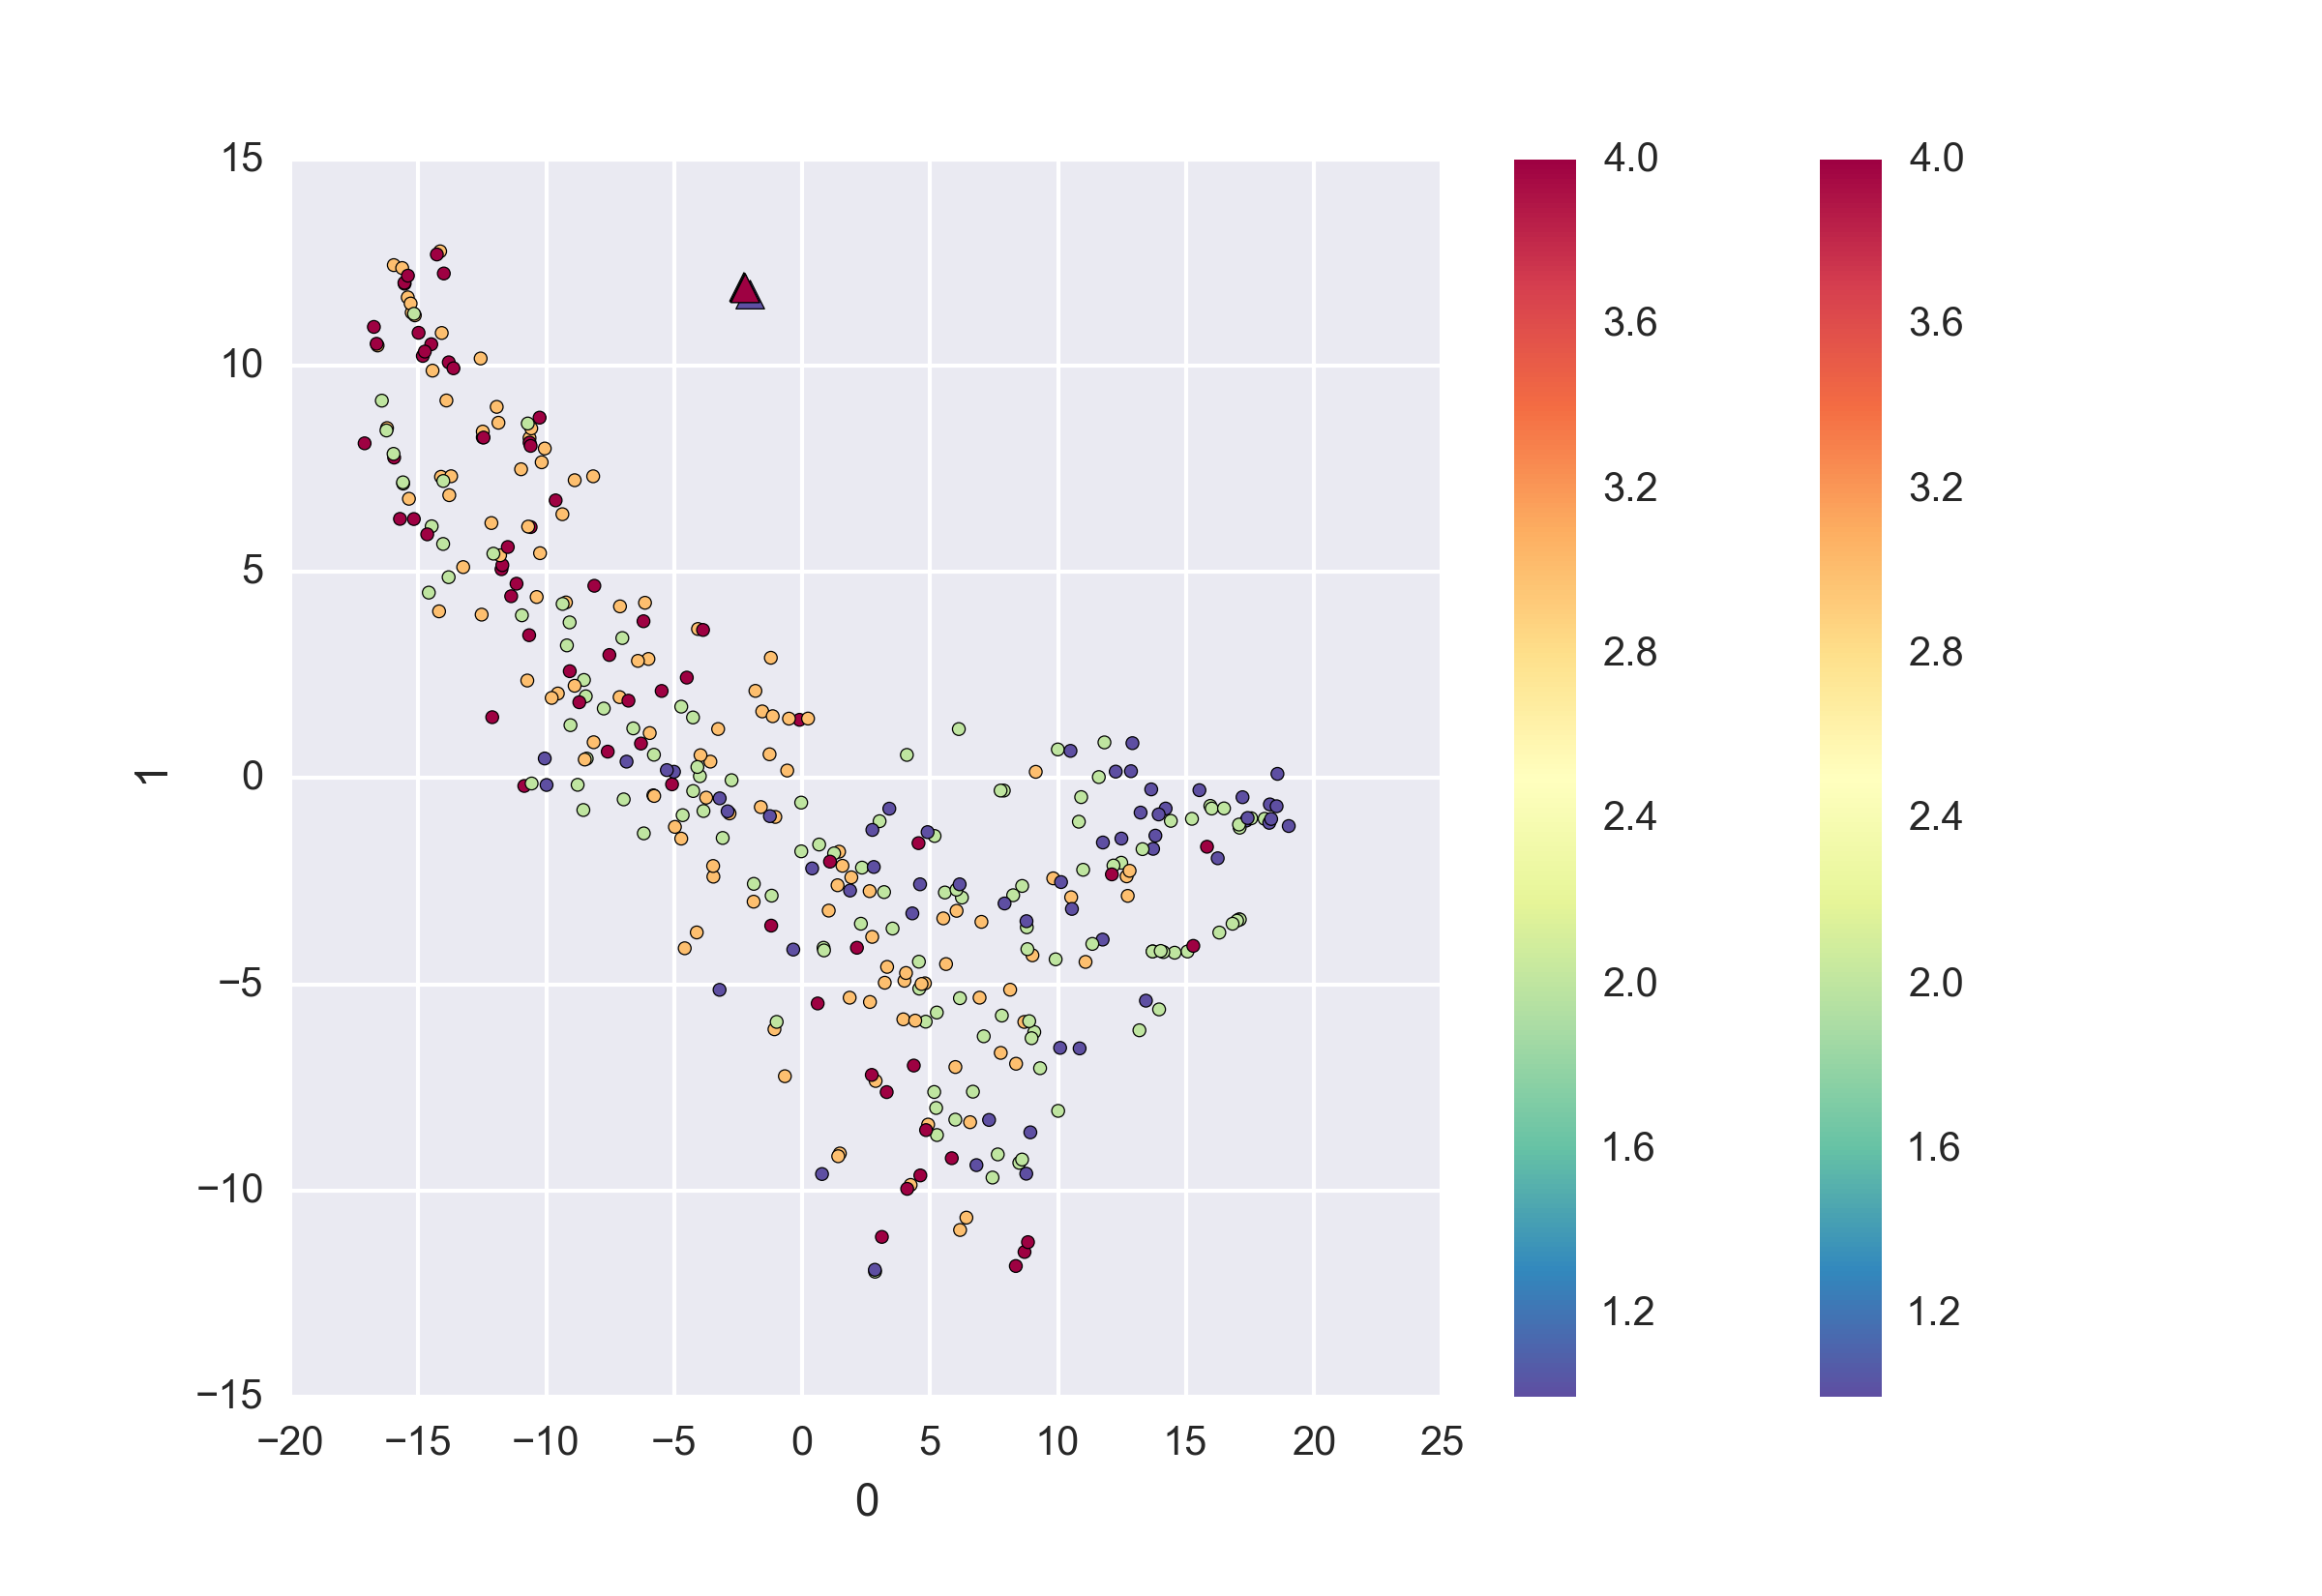
\includegraphics[width=0.4\textwidth]{figures/mappings/texture_SNE_mapping_2d.png}}
	\subfigure{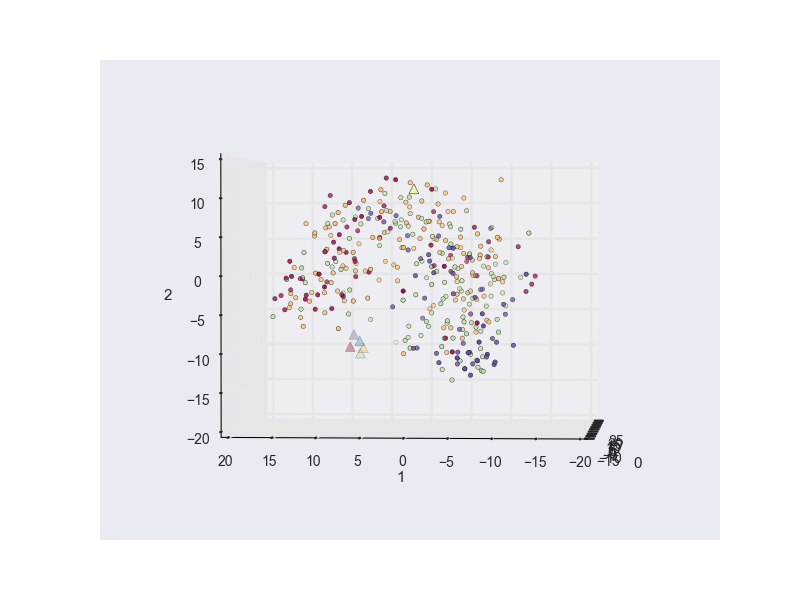
\includegraphics[width=0.49\textwidth]{figures/mappings/texture_SNE_mapping_3d.png}}
	\caption{2D \& 3D projections of the texture feature space generated from blobs generated from blobs produced by the t-SNE algorithm with a learning rate of 200 and perplexity of 20.}\label{fig:texture_SNE_mapping}
\end{figure}

\begin{figure}[H]
	\centering
	\subfigure{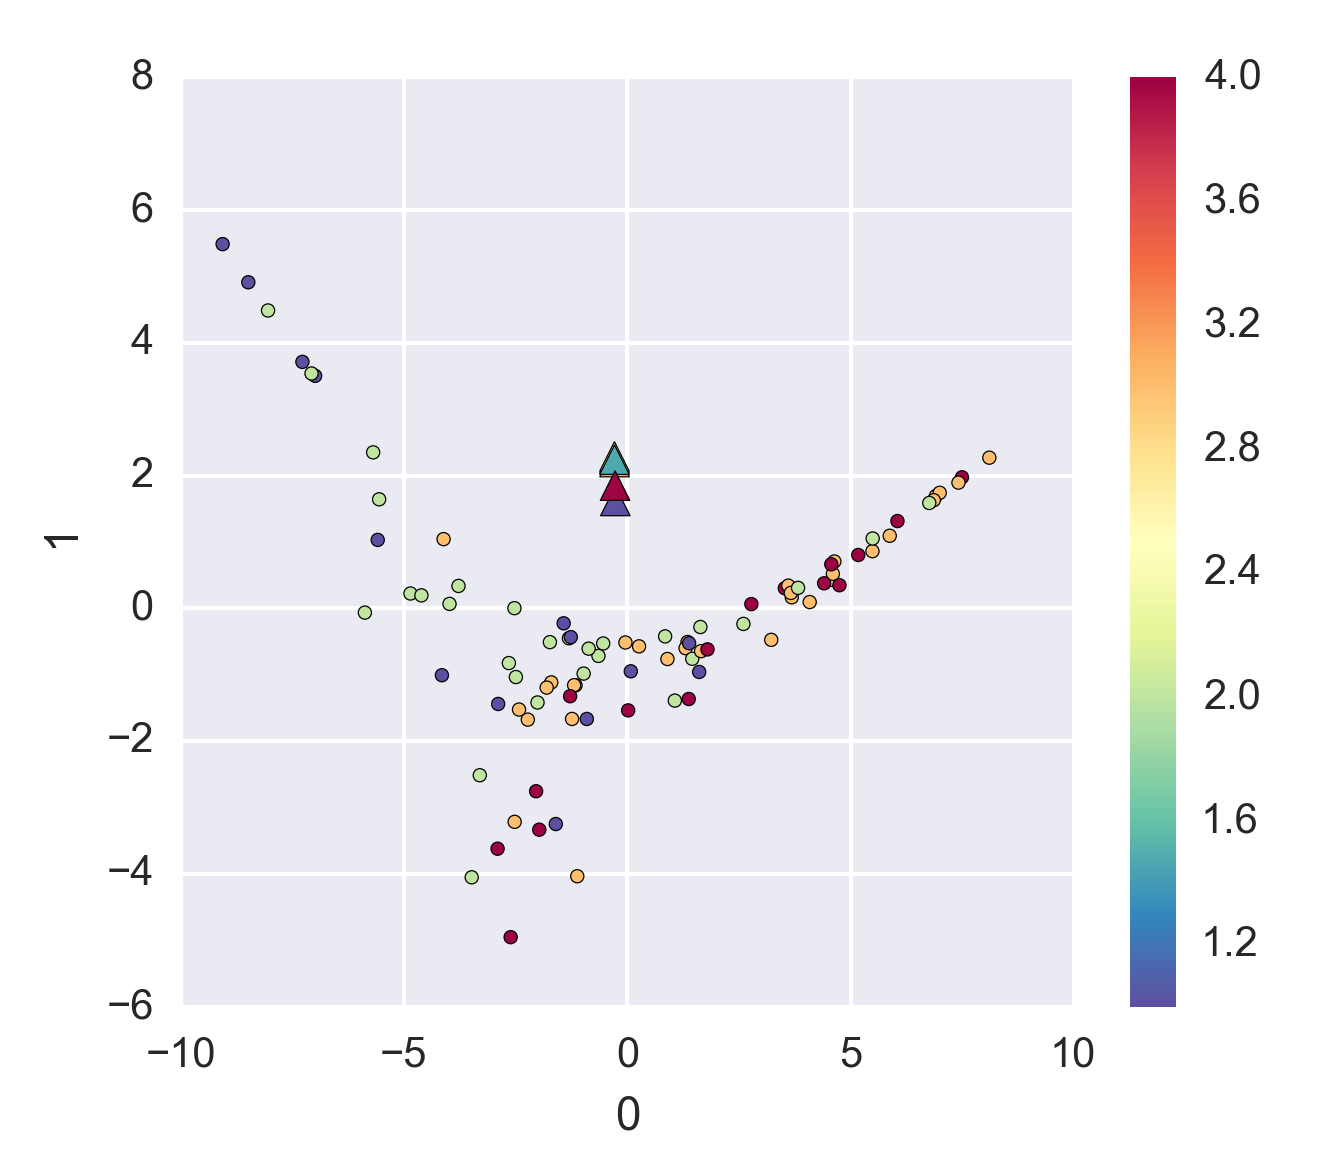
\includegraphics[width=0.4\textwidth]{figures/mappings/texture_iso_mapping_2d.png}}
	\subfigure{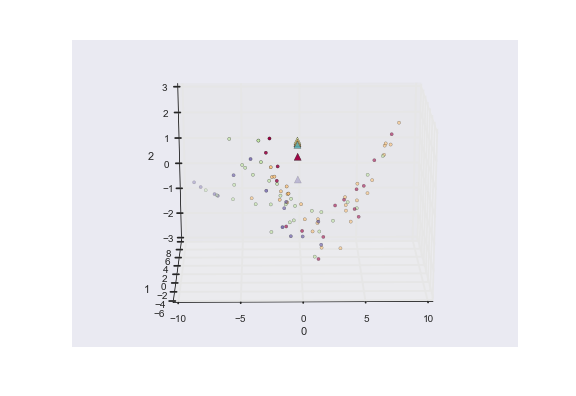
\includegraphics[width=0.49\textwidth]{figures/mappings/texture_iso_mapping_3d.png}}
	\caption{2D \& 3D projections of the texture feature space generated from blobs produced by the Isomap algorithm with 4 neighbours.}\label{fig:texture_iso_mapping}
\end{figure}

\begin{figure}[H]
	\centering
	\subfigure{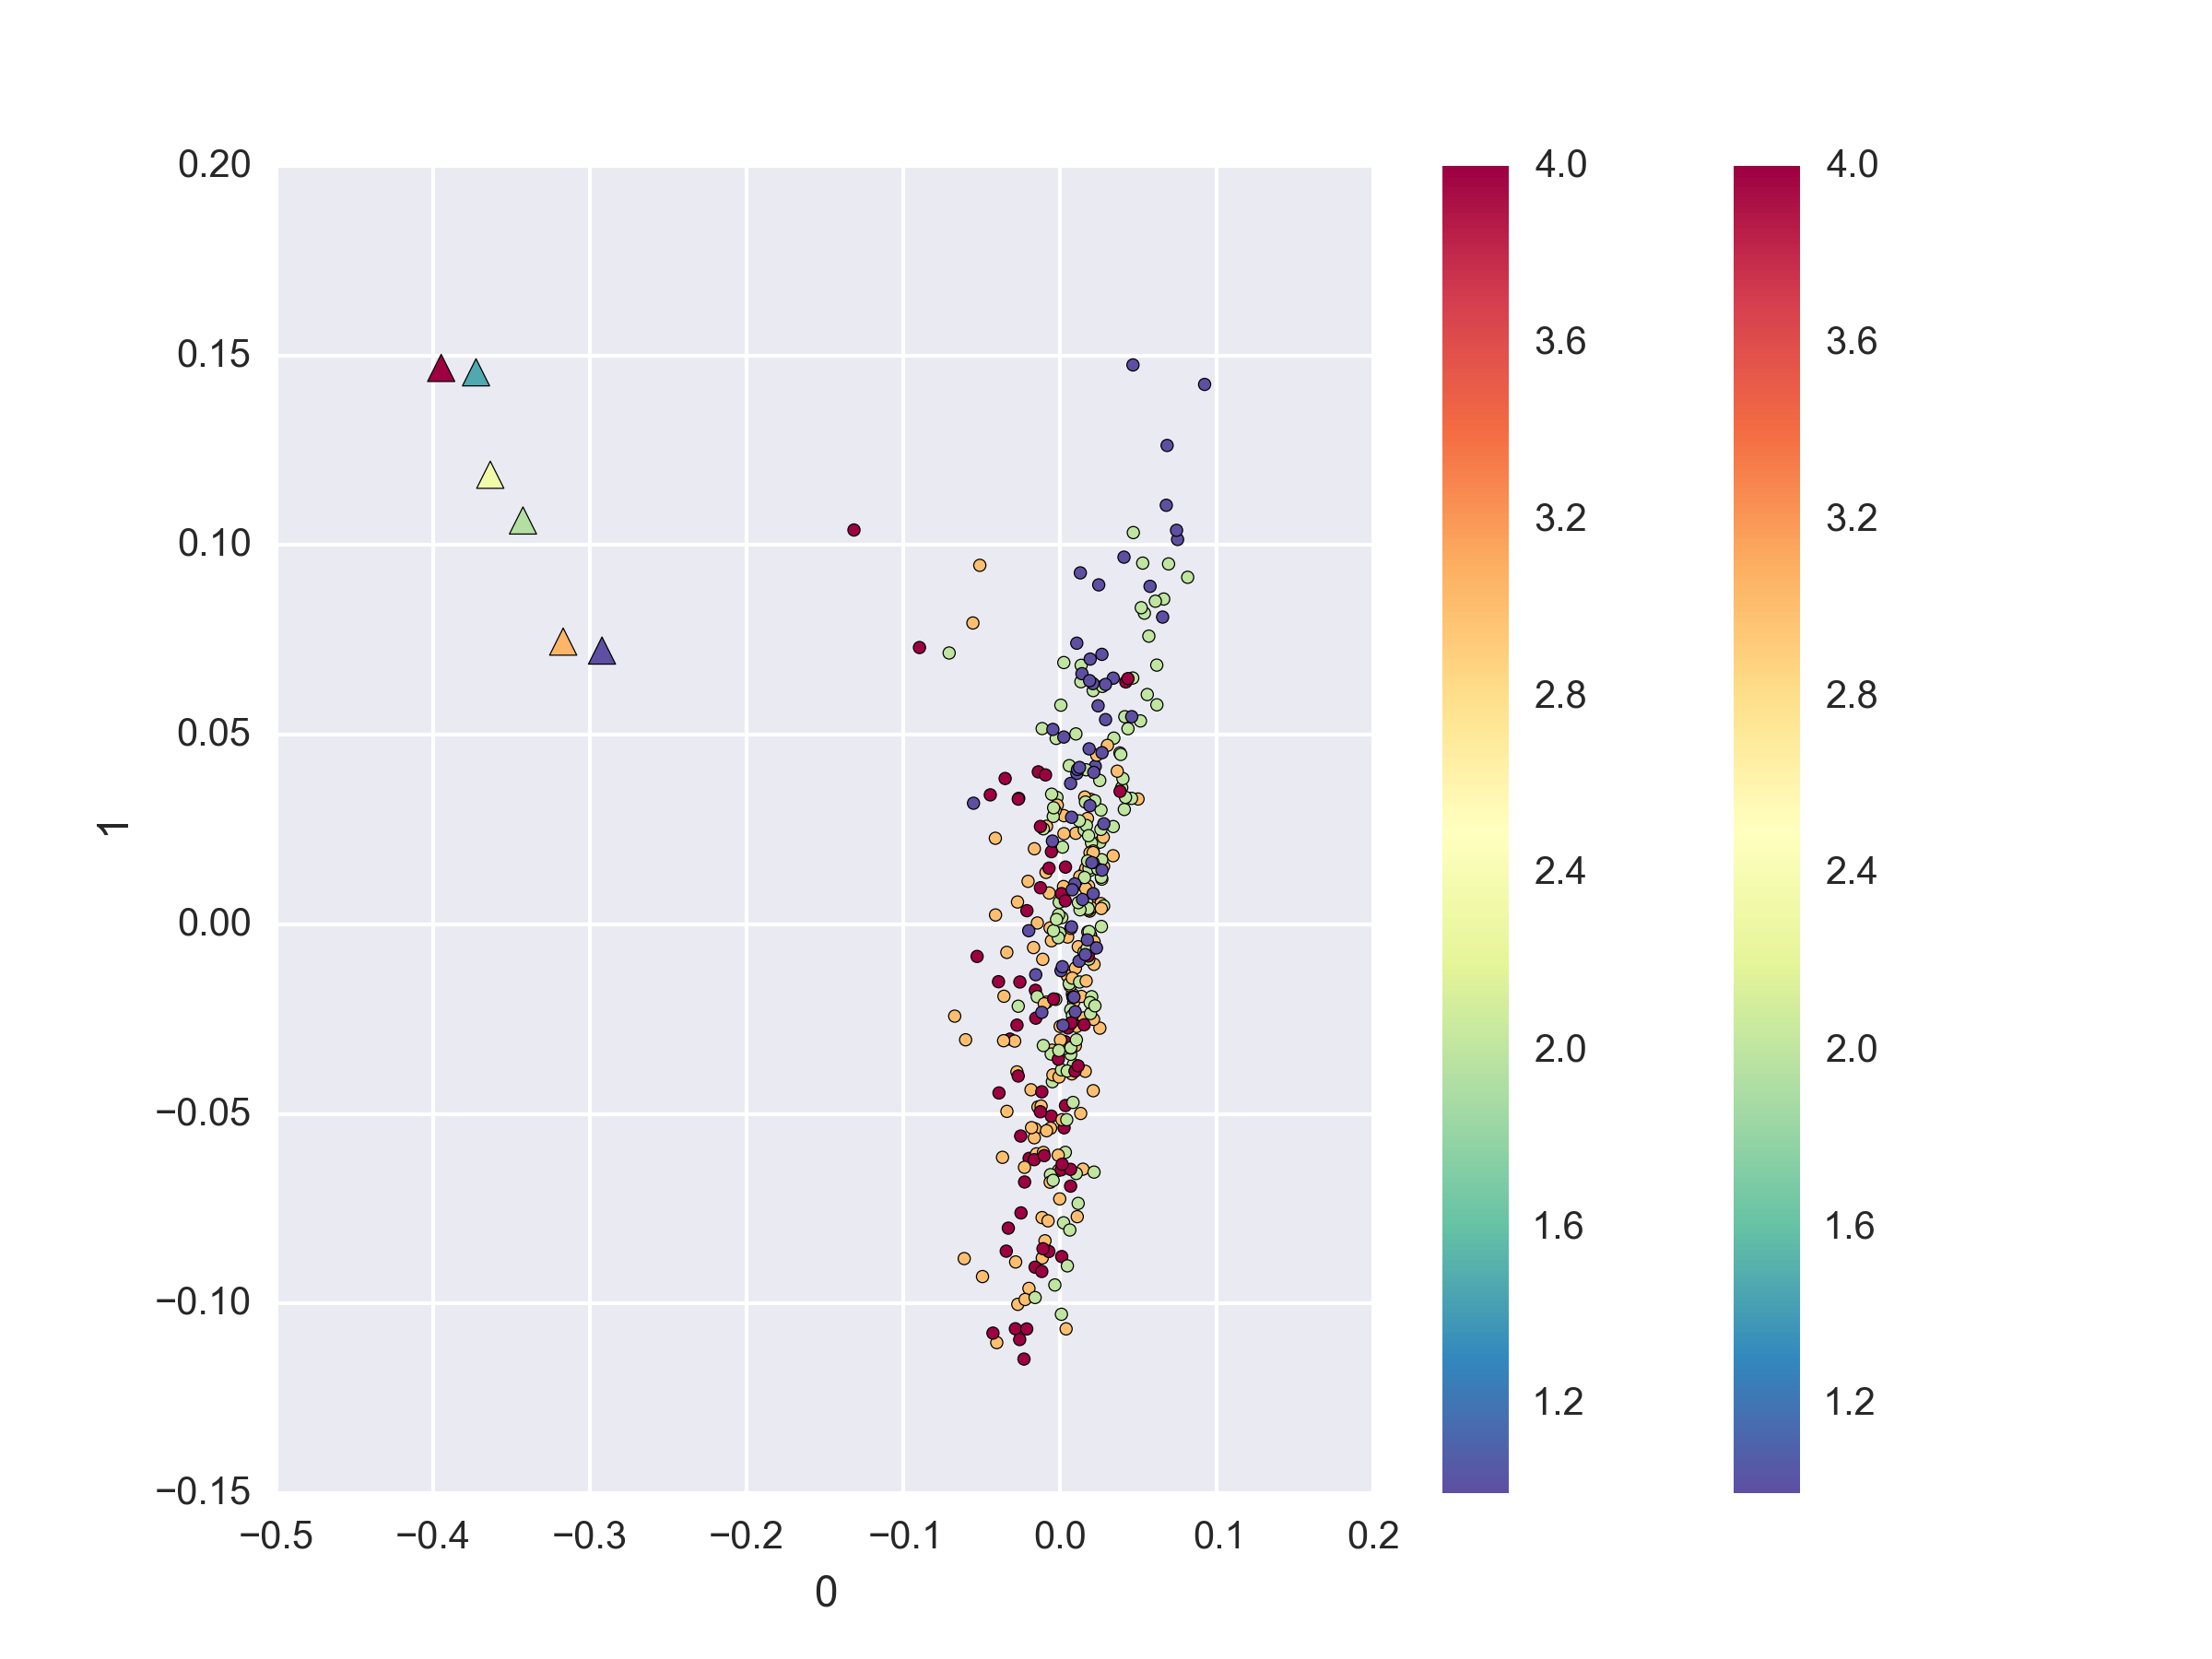
\includegraphics[width=0.4\textwidth]{figures/mappings/texture_lle_mapping_2d.png}}
	\subfigure{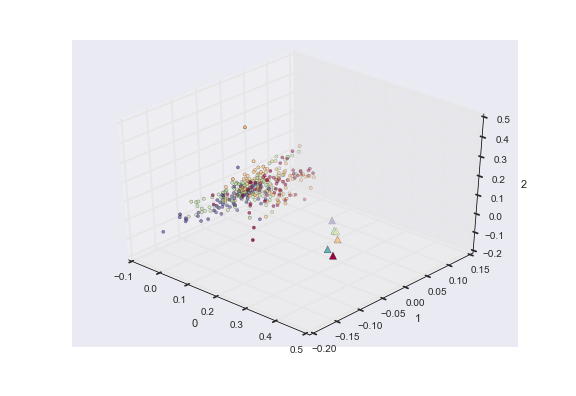
\includegraphics[width=0.49\textwidth]{figures/mappings/texture_lle_mapping_3d.png}}
	\caption{2D \& 3D projections of the texture feature space generated from blobs produced by the LLE algorithm with 4 neighbours.}\label{fig:texture_LLE_mapping}
\end{figure}
\clearpage

% Quality for blob texture features
%------------------------------------------------------------------------------------

\clearpage
\begin{figure}[H]
	\centering
	\subfigure{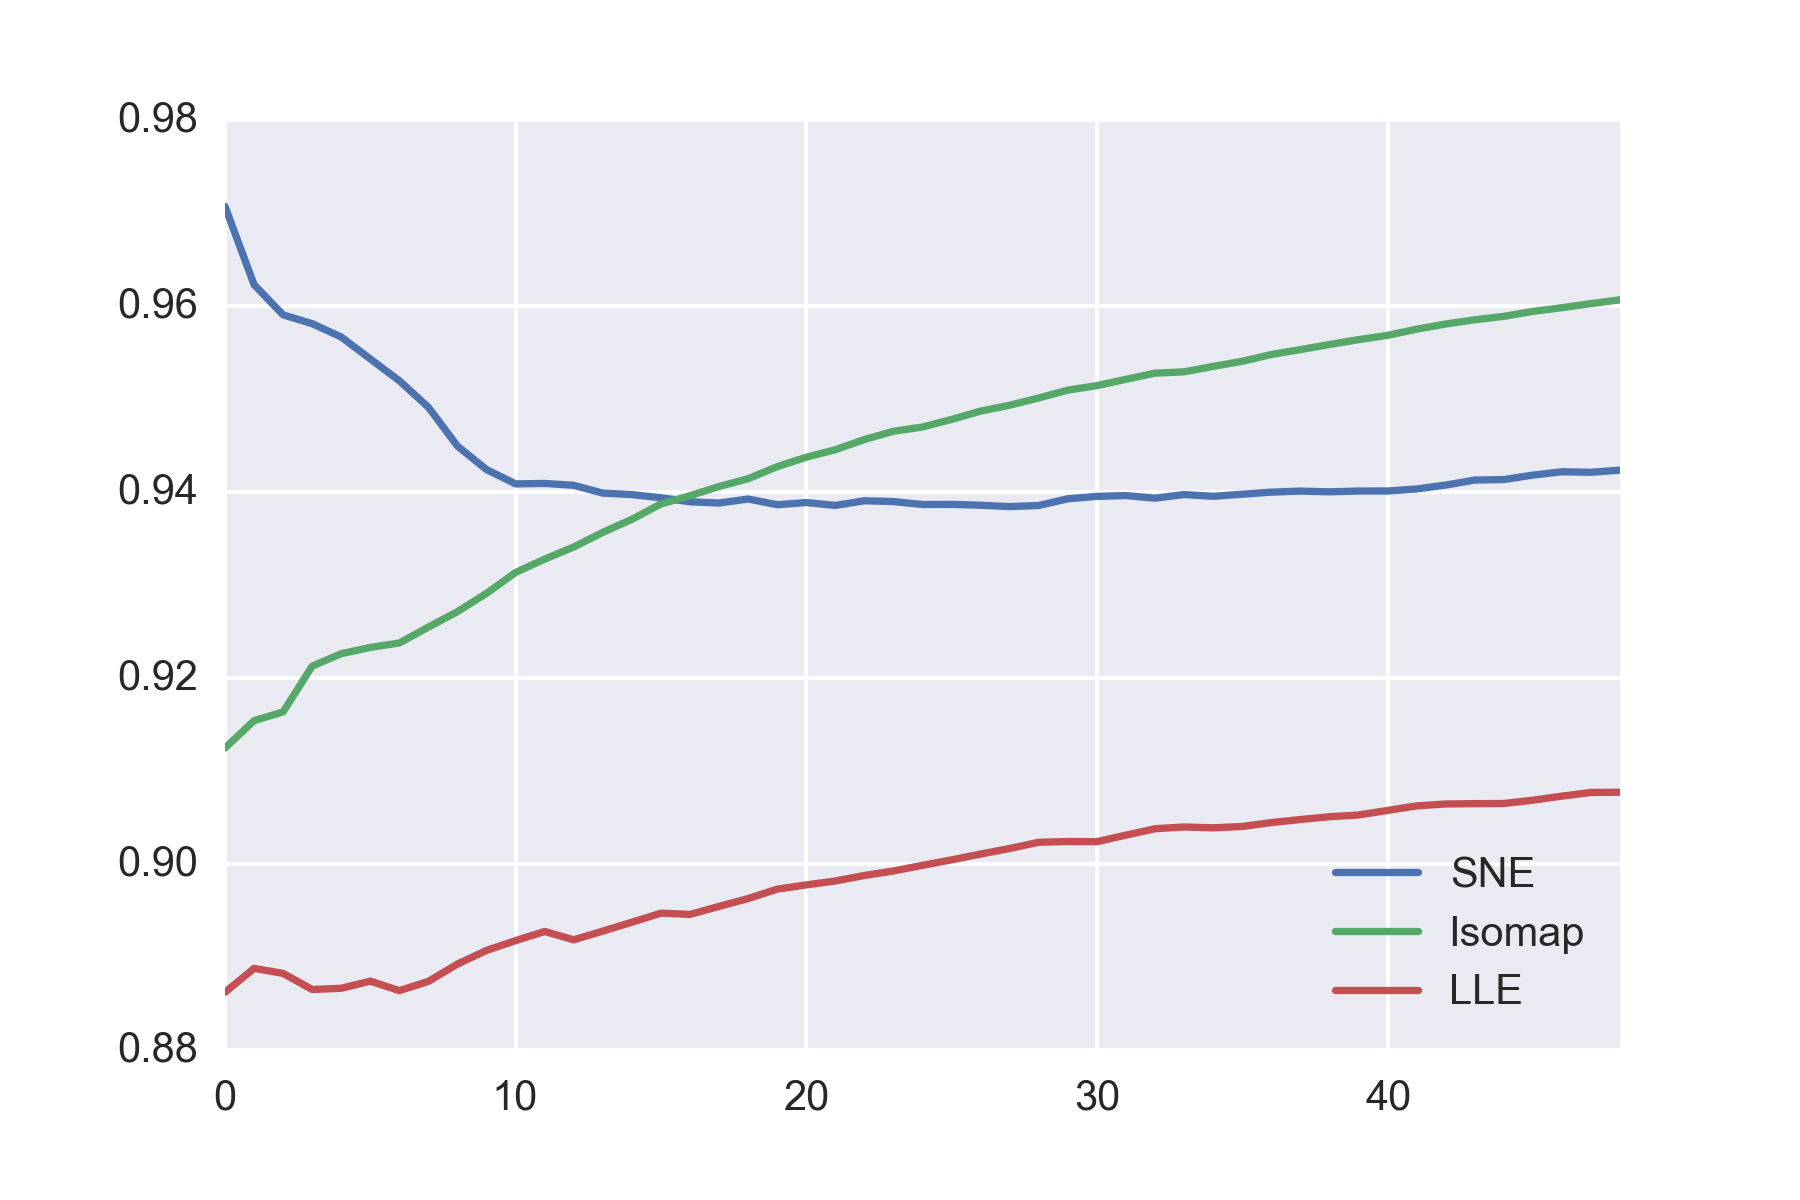
\includegraphics[width=0.49\textwidth]{figures/quality_measures/texture_trustworthiness_2d.png}}
	\subfigure{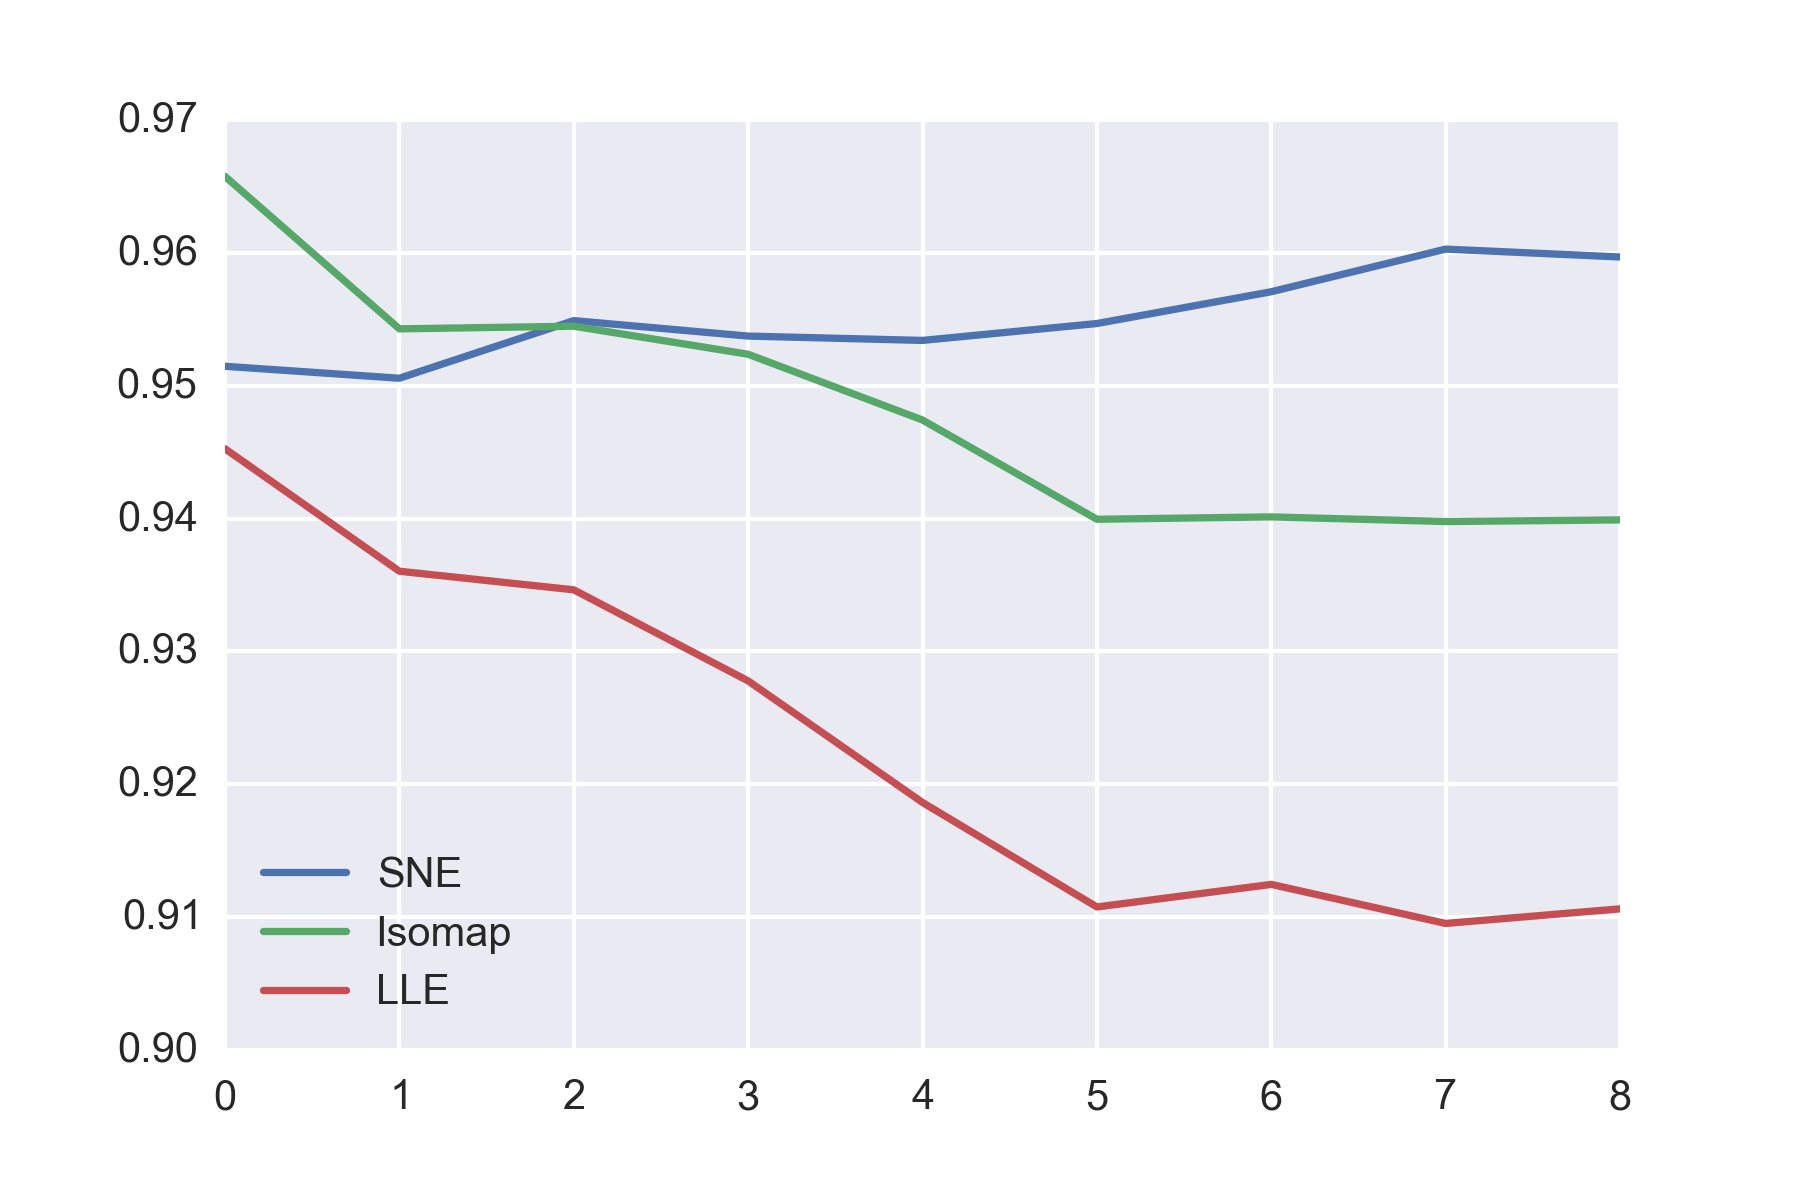
\includegraphics[width=0.49\textwidth]{figures/quality_measures/texture_continuity_2d.png}}
	\caption{Trustworthiness (left) and continuity (right) of the 2D projections produced from texture features from blobs.}\label{fig:TC_2d_texture}
\end{figure}

\begin{figure}[H]
	\centering
	\subfigure{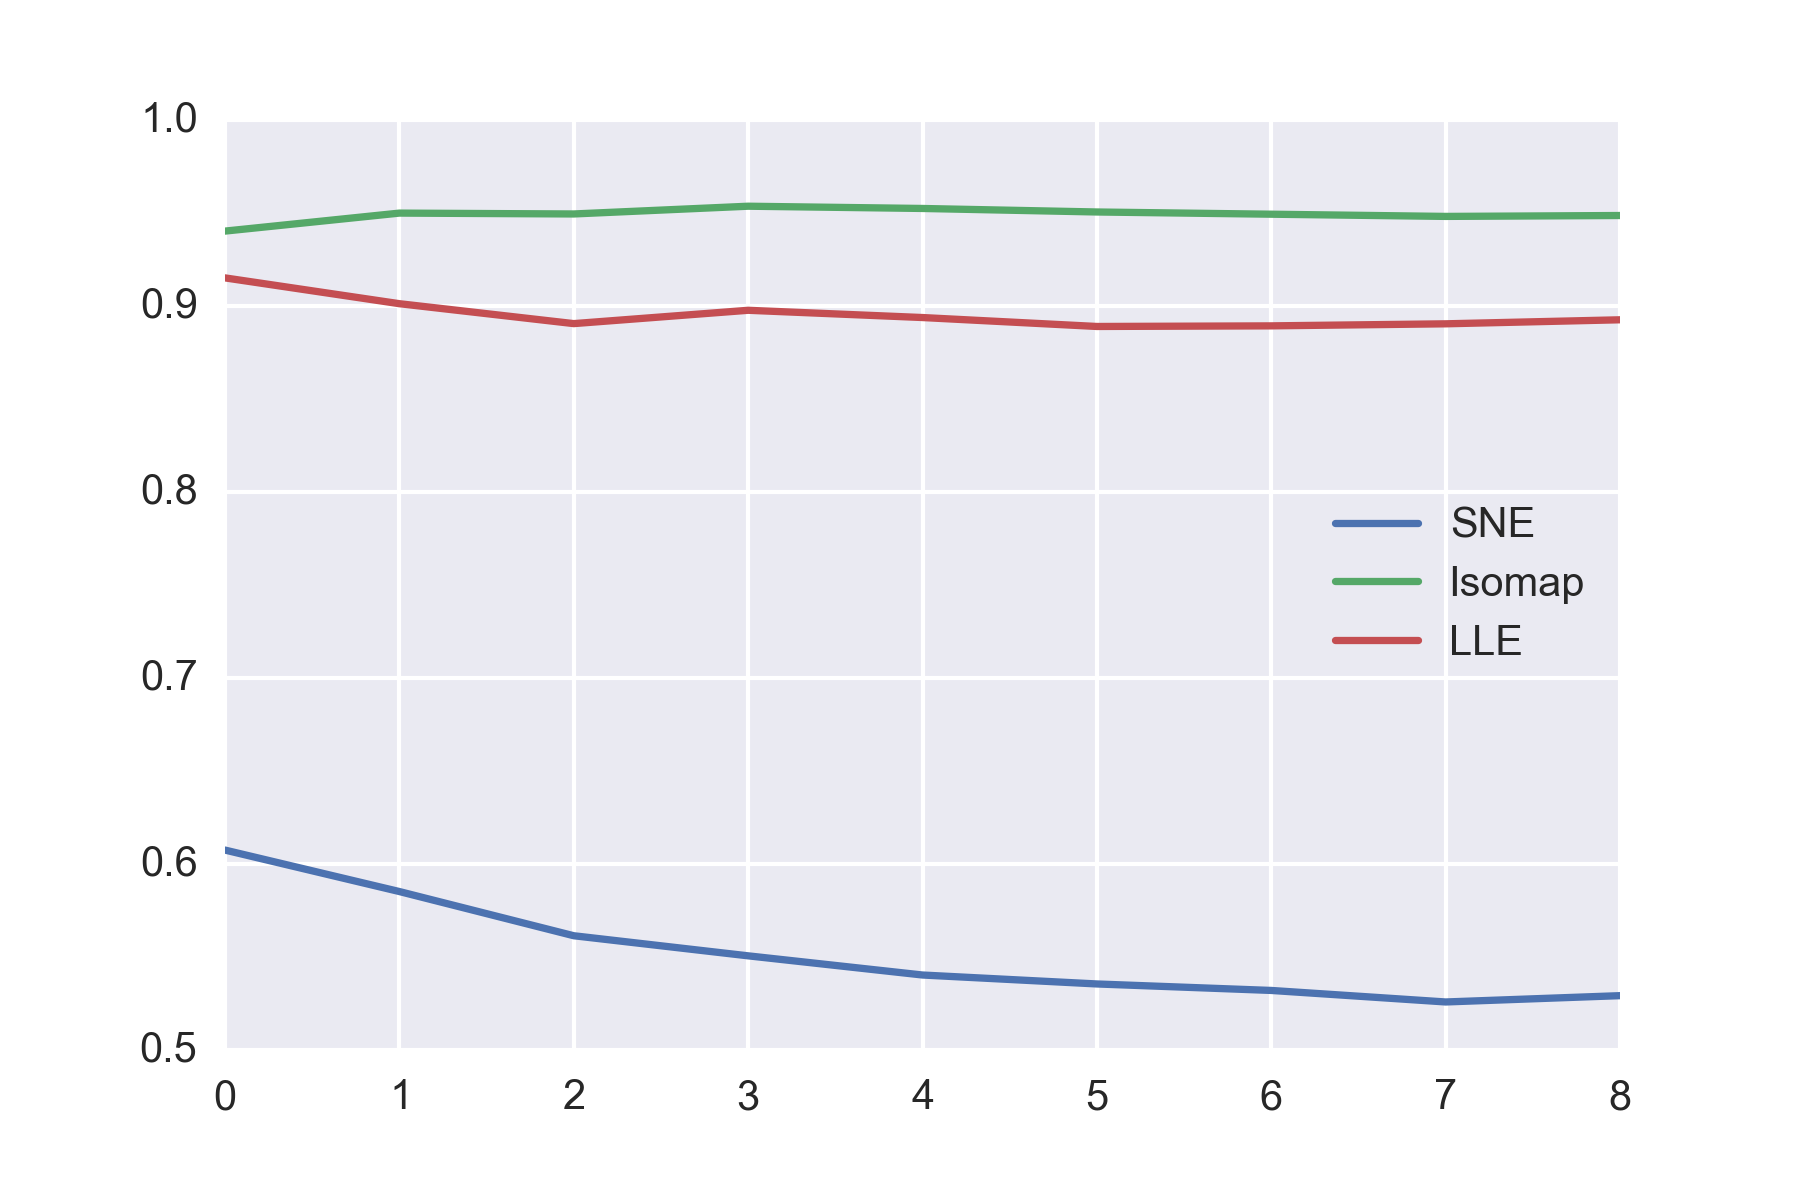
\includegraphics[width=0.49\textwidth]{figures/quality_measures/texture_trustworthiness_3d.png}}
	\subfigure{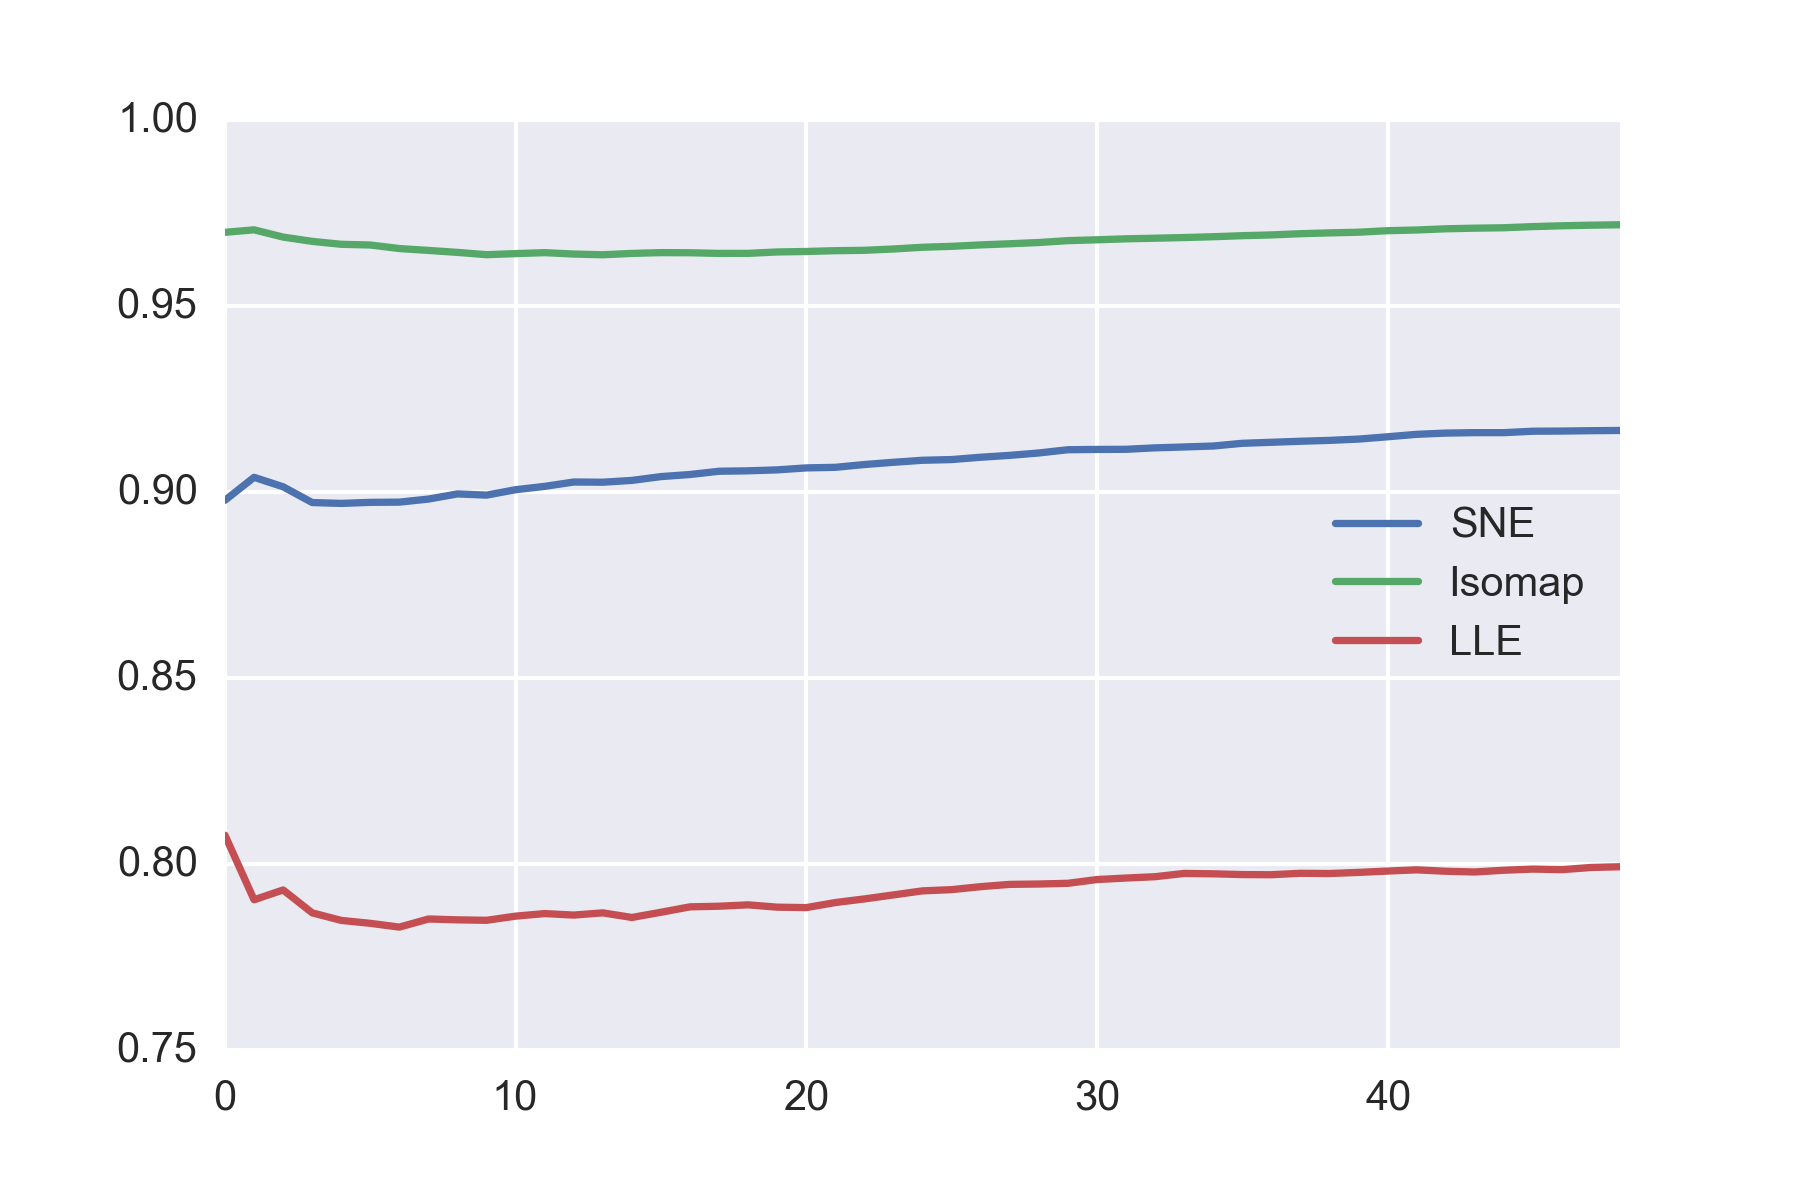
\includegraphics[width=0.49\textwidth]{figures/quality_measures/texture_continuity_3d.png}}
	\caption{Trustworthiness (left) and continuity (right) of the 3D projections produced from texture features from blobs.}\label{fig:TC_3d_texture}
\end{figure}

\begin{figure}[H]
	\centering
	\subfigure{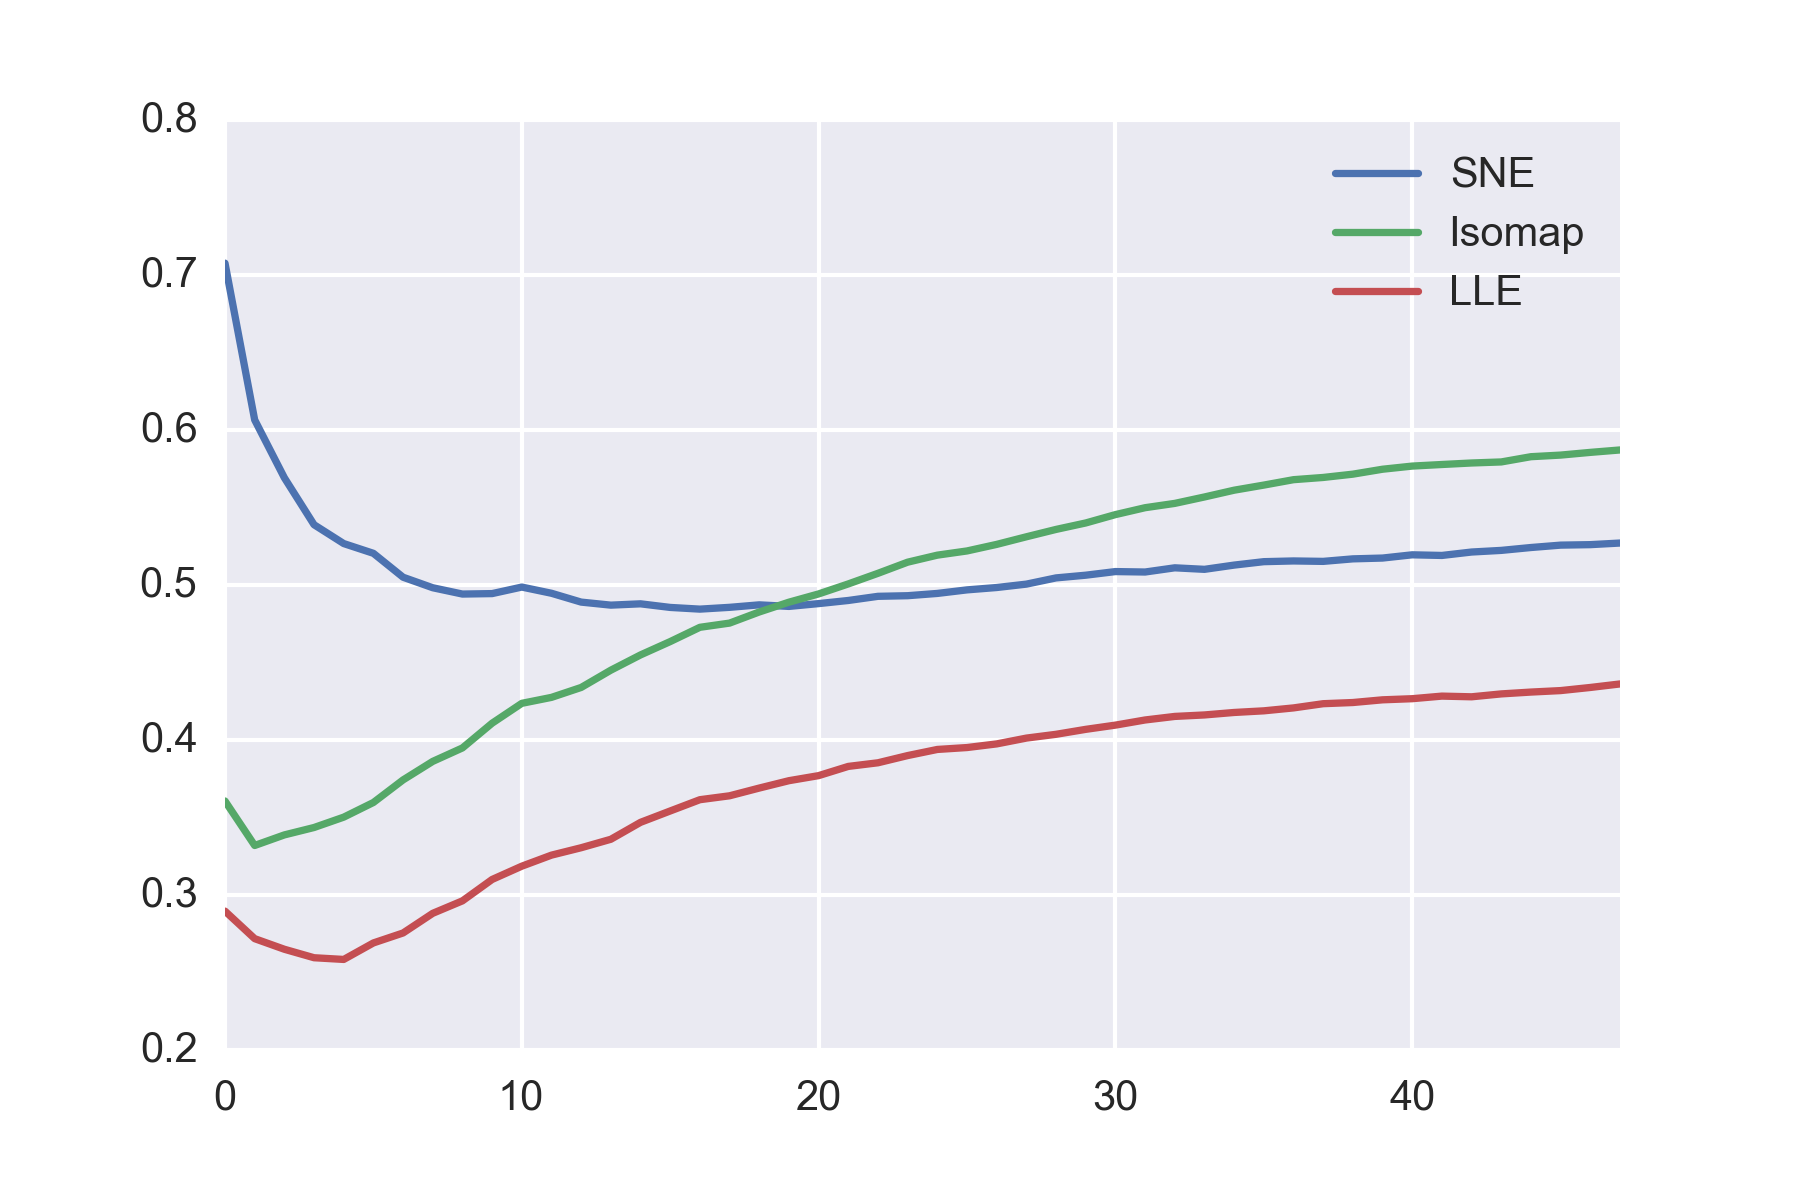
\includegraphics[width=0.49\textwidth]{figures/quality_measures/texture_lcmc_2d.png}}
	\subfigure{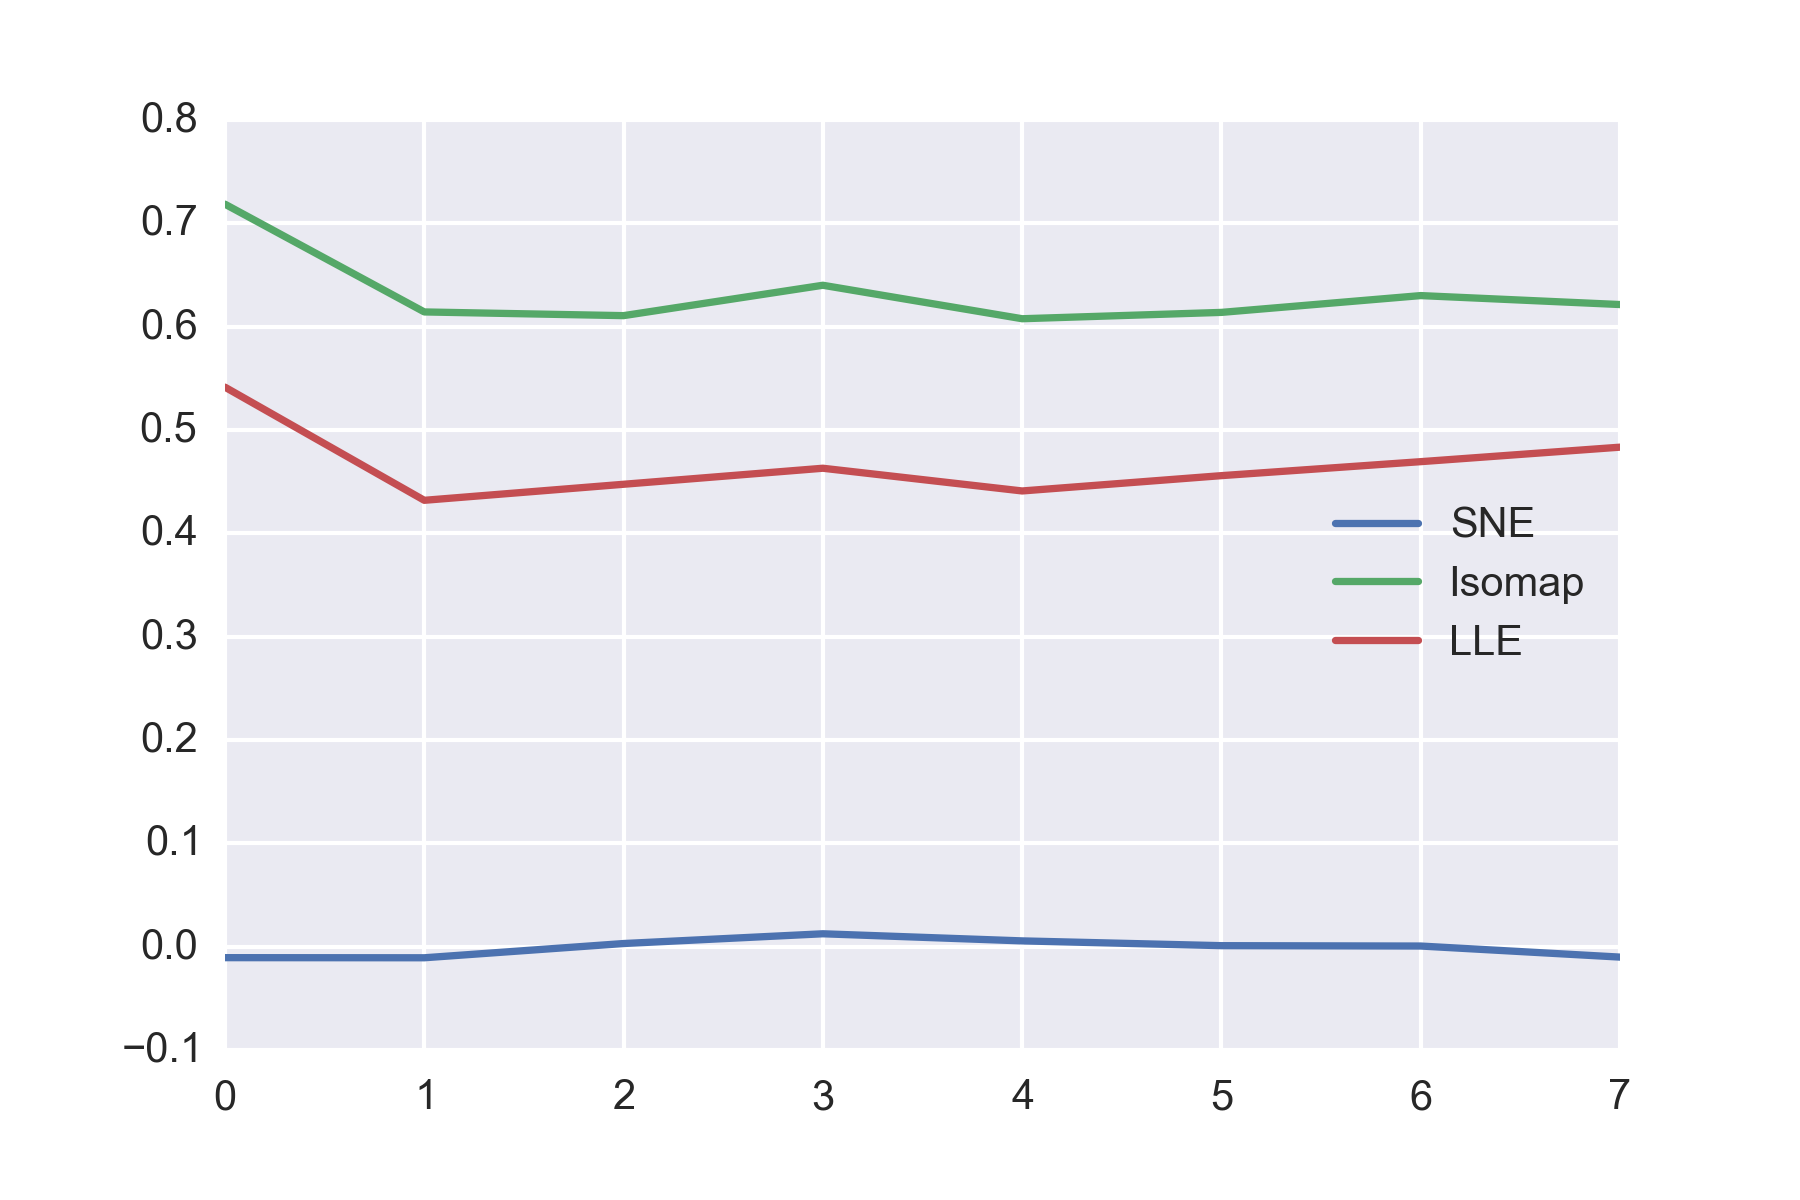
\includegraphics[width=0.49\textwidth]{figures/quality_measures/texture_lcmc_3d.png}}
	\caption{LCMC of both the 2D projection (left) and 3D projection (right) of the feature space for texture.}\label{fig:LCMC_texture}
\end{figure}
\clearpage

%------------------------------------------------------------------------------------
% Line intensity and texture features
%------------------------------------------------------------------------------------

\clearpage
\begin{figure}[H]
	\centering
	\subfigure{\includegraphics[width=0.4\textwidth]{figures/mappings/line_intensity_SNE_mapping_2d.png}}
	\subfigure{\includegraphics[width=0.49\textwidth]{figures/mappings/line_intensity_SNE_mapping_3d.png}}
	\caption{2D \& 3D projections of the intensity feature space for lines produced by the t-SNE algorithm with a learning rate of 200 and perplexity of 20.}\label{fig:intensity_SNE_mapping_lines}
\end{figure}

\begin{figure}[H]
	\centering
	\subfigure{\includegraphics[width=0.4\textwidth]{figures/mappings/line_intensity_iso_mapping_2d.png}}
	\subfigure{\includegraphics[width=0.49\textwidth]{figures/mappings/line_intensity_iso_mapping_3d.png}}
	\caption{2D \& 3D projections of the intensity feature space generated from lines produced by the Isomap algorithm with 4 neighbours.}\label{fig:intensity_iso_mapping_lines}
\end{figure}

\begin{figure}[H]
	\centering
	\subfigure{\includegraphics[width=0.4\textwidth]{figures/mappings/line_intensity_lle_mapping_2d.png}}
	\subfigure{\includegraphics[width=0.49\textwidth]{figures/mappings/line_intensity_lle_mapping_3d.png}}
	\caption{2D \& 3D projections of the intensity feature space for lines generated from blobs produced by the LLE algorithm with 4 neighbours.}\label{fig:intensity_LLE_mapping_lines}
\end{figure}
\clearpage


% Quality for line intensity features
%------------------------------------------------------------------------------------
\clearpage
\begin{figure}[H]
	\centering
	\subfigure{\includegraphics[width=0.49\textwidth]{figures/quality_measures/line_intensity_trustworthiness_2d.png}}
	\subfigure{\includegraphics[width=0.49\textwidth]{figures/quality_measures/line_intensity_continuity_2d.png}}
	\caption{Trustworthiness (left) and continuity (right) of the 2D projections produced from intensity features from lines.}\label{fig:TC_2d_intensity}
\end{figure}

\begin{figure}[H]
	\centering
	\subfigure{\includegraphics[width=0.49\textwidth]{figures/quality_measures/line_intensity_trustworthiness_3d.png}}
	\subfigure{\includegraphics[width=0.49\textwidth]{figures/quality_measures/line_intensity_continuity_3d.png}}
	\caption{Trustworthiness (left) and continuity (right) of the 3D projections produced from intensity features from lines.}\label{fig:TC_3d_intensity}
\end{figure}

\begin{figure}[H]
	\centering
	\subfigure{\includegraphics[width=0.49\textwidth]{figures/quality_measures/line_intensity_lcmc_2d.png}}
	\subfigure{\includegraphics[width=0.49\textwidth]{figures/quality_measures/line_intensity_lcmc_3d.png}}
	\caption{LCMC of both the 2D projection (left) and 3D projection (right) of the feature space for intensity from lines.}\label{fig:LCMC_intensity}
\end{figure}
\clearpage


\clearpage
\begin{figure}[H]
	\centering
	\subfigure{\includegraphics[width=0.4\textwidth]{figures/mappings/lines_texture_SNE_mapping_2d.png}}
	\subfigure{\includegraphics[width=0.49\textwidth]{figures/mappings/lines_texture_SNE_mapping_3d.png}}
	\caption{2D \& 3D projections of the texture feature space generated generated from lines produced by the t-SNE algorithm with a learning rate of 200 and perplexity of 20.}\label{fig:texture_SNE_mapping_lines}
\end{figure}

\begin{figure}[H]
	\centering
	\subfigure{\includegraphics[width=0.4\textwidth]{figures/mappings/lines_texture_iso_mapping_2d.png}}
	\subfigure{\includegraphics[width=0.49\textwidth]{figures/mappings/lines_texture_iso_mapping_3d.png}}
	\caption{2D \& 3D projections of the texture feature space generated from lines produced by the Isomap algorithm with 4 neighbours.}\label{fig:texture_iso_mapping_lines}
\end{figure}

\begin{figure}[H]
	\centering
	\subfigure{\includegraphics[width=0.4\textwidth]{figures/mappings/lines_texture_lle_mapping_2d.png}}
	\subfigure{\includegraphics[width=0.49\textwidth]{figures/mappings/lines_texture_lle_mapping_3d.png}}
	\caption{2D \& 3D projections of the texture feature space generated from lines produced by the LLE algorithm with 4 neighbours.}\label{fig:texture_LLE_mapping_lines}
\end{figure}
\clearpage

% Quality for line texture features
%------------------------------------------------------------------------------------

\clearpage
\begin{figure}[H]
	\centering
	\subfigure{\includegraphics[width=0.49\textwidth]{figures/quality_measures/lines_texture_trustworthiness_2d.png}}
	\subfigure{\includegraphics[width=0.49\textwidth]{figures/quality_measures/lines_texture_continuity_2d.png}}
	\caption{Trustworthiness (left) and continuity (right) of the 2D projections produced from texture features from lines.}\label{fig:TC_2d_texture}
\end{figure}

\begin{figure}[H]
	\centering
	\subfigure{\includegraphics[width=0.49\textwidth]{figures/quality_measures/lines_texture_trustworthiness_3d.png}}
	\subfigure{\includegraphics[width=0.49\textwidth]{figures/quality_measures/lines_texture_continuity_3d.png}}
	\caption{Trustworthiness (left) and continuity (right) of the 3D projections produced from texture features from lines.}\label{fig:TC_3d_texture}
\end{figure}

\begin{figure}[H]
	\centering
	\subfigure{\includegraphics[width=0.49\textwidth]{figures/quality_measures/lines_texture_lcmc_2d.png}}
	\subfigure{\includegraphics[width=0.49\textwidth]{figures/quality_measures/lines_texture_lcmc_3d.png}}
	\caption{LCMC of both the 2D projection (left) and 3D projection (right) of the feature space from lines for texture.}\label{fig:LCMC_texture}
\end{figure}
\clearpage


\section{Conclusions}
In summary, it can be concluded that the synthetic mammograms used as part of this experiment are not significantly related to real mammograms in terms of the features derived during this study. The synthetic mammograms appear to be closest to real mammograms in terms of the shape of the structures present in the image. The best results from this experiment were derived from the feature space of multi-scale blobs. Line features also seemed to positively show the the real and synthetic mammograms are at least in the same space in terms of shape. However, texture and intensity features derived from either of the features clearly show that the two datasets are not in the same intensity space. The two sample KS test confirms that the features created from both datasets are statistically not drawn from the same distribution and therefore we must conclude that they are, for all features presented here, effectively different.

This conclusion roughly correlates with the limitations discussed by the authors of the synthetic data \cite{bakic2002mammogram1, bakic2002mammogram2, bakic2003mammogram3}. They state that the synthetic mammograms are closest to real mammograms in terms of shape but are not so close in terms of intensity and texture. In the experiments with shape features presented here the major difference between the real and synthetic mammograms was caused by a lack of small scale structure being detected in the synthetic mammograms. This causes them to be grouped in with mammograms which are deemed to be of higher risk, regardless of their effective risk, because of the lack of small blob counts detected. The same can be said for line features where the number and size of lines is generally smaller, regardless of the risk.

The quality evaluation of the visualisations produced suggests that Isomap produces visualisations which best capture the local neighbourhood structure of mappings. t-SNE appears to often show similar levels of faithfulness in compared to Isomap in two dimensions, but was shown to be much worse for three dimensions.



\chapter{Critical Evaluation}
This final chapter presents my evaluation of the project as a whole, outlines directions for future work in this area and provides a personal reflection on how I have handled and executed this project.

\section{Evaluation of the Project}
Overall this project has managed to answer some of the original questions laid out during the problem analysis and I feel that while the results of this project are not necessarily  as good as I was hoping for this has still been a fun project and excellent learning experience. I started this project with very minimal knowledge of image processing and analysis techniques (other than what had been taught in other university modules) and no knowledge of dimensionality reduction algorithms. I also started this project with very little prior knowledge of linear algebra, something which I would call a prerequisite for properly understanding many dimensionality reduction algorithms.

There were several goals that I set out to achieve as part of this project. This section will discuss them one by one and provide a review of what was achieved, what went well, and what went wrong.

The first goal was to generate image features from both real and synthetic mammogram images based on a variety of common techniques used with mammographic images. This required an extensive review of existing literature on the subject and the selection of a few techniques from each case to be used as part of the final system pipeline.

I feel that the features chosen for use in this project were entirely appropriate. I feel that starting with shape based features was a good idea and that the two techniques chosen produced reasonable results in practice. Blob features proved more complicated to implement than line features overall, but blob features end up producing better results and so I felt the extra effort involved was justified. 

After extracting shape features I wanted to also try and focus on extracting other types of feature from the images. A difficult issue with this the time complexity required to extract more complicated features (i.e. texture features) from an image. For this reason I chose to use the patch of image defined by shape features as way narrow down the amount of processing required on each image. The reasoning behind this was that because a ROI has already been defined, extracting texture and intensity features from that region might be a good point to focus on.

In hindsight to this project I feel that I should have only focussed on an single type of image features (such as shape based). There were a lot of different pieces to this project outside of pure implementation and I think that I would of had a much more well-polished project had I narrowed the project scope.

My biggest regret with feature extraction is that I didn't realise until after the extracting texture and intensity features that the intensity distribution between real and synthetic images is very different, leading to the clear separation between the two datasets that can be viewed in all of the visualisations of these spaces. While this proved to be a disappointing result it does match with the some of the limitations proposed by the authors of the synthetic dataset in refs. \cite{bakic2002mammogram1, bakic2002mammogram2, bakic2003mammogram3}. In terms of the shape features, the synthetic mammograms at least appeared to be in the same space as their real counterparts but the extracted features were still unable to properly align the synthetics under projection according to their associated level of risk.

The second goal was to perform dimensionality reduction on the feature space generated by each of these techniques to produce two and three dimensional visual representations. A variety of different techniques were investigated as part of the initial stage of this project and a few fundamentally different approaches were selected to be used in the results of this project.

As I have briefly mentioning in the first paragraph of this section, one of the major challenges that I felt I faced with this project was trying fully understand the core principles and mathematics behind how dimensionality reduction algorithms worked. This was an area in which I had zero knowledge of before I began this project and subsequently I spent a significant proportion of the early part of the project researching how some of the more common techniques work along with the strengths and weaknesses of each. 

There was very little technical effort involved with this component of the project. All of the techniques used in the project were already implemented as part of the scikit-learn python library. I felt that there was no need to reimplement complicated dimensionality reduction algorithms when they were already readily available in a well known and well tested package. I feel that the choice of dimensionality reduction techniques used was justified and that a small yet diverse mix of approaches were presented along with the results.

The third goal was to produce a way of evaluating the quality of the visualisations produced by dimensionality reduction. Once again this was investigated as part of the initial stage of the project and quality metrics derived from co-ranking matrices were eventually selected as the best choice due to the large number of measures that can be derived from them.

Again, like dimensionality reduction, this was an area that required more background reading than actual implementation. The implementation of the co-ranking matrix and the measures derived from it are actually only a few hundred lines of code, but understanding how the co-ranking matrix is derived and what the metrics subsequently derived from it measure took the majority of the effort. I felt that this was a justified approach to assess the quality of the mappings produced but that there was much more that could have been done in this area, for example in visualising the quality of the mapping in a similar way as suggested by Mokbel et al \cite{mokbel2013visualizing}.

The third aim was to integrate these separate components into an image analysis pipeline. This goal was achieved as part of a Python package produced during this project. While the implementation offered in this package is far from perfect I feel that it provides a good basic implementation of a image analysis pipeline. I feel that the most well developed part of the system is the feature extraction component. This provides reusable way to implement new feature detection routines through an interface that provides support for multiprocessing on a per image basis.

There are, however, some parts of the system I am not entirely happy with. The most notable of these is the section analysis module. This has mostly been developed on an ad-hoc basis depending on the functions I required to perform analysis. This module has ended up being a collection of the more common operations used when processing the features using IPython notebooks. It was particularly difficult deciding which functions to include in this module. The problem is that the operations you need to perform on the data largely depends on the patterns you see in the data itself. On one hand obviously not every single thing should be included, but on the other the aim of good software is to produce reusable components. Based on this I chose to work on the code in an IPython notebook and if I required the function in more than one place, move it into the analysis module.

The final aim of this project was to try and examine the difference between projections of the feature space of real and synthetic mammogram datasets. In this goal I feel that I have only been partially successful. While I feel that the results of the experiments performed allow us to draw some valid conclusions about the the differences between the two datasets I also feel that I could have spent more time constructing a better system to evaluate the results.

I feel that by far my most major weakness in the project was failing to full develop how to formally compare the feature spaces generated by the two datasets. Throughout the project my analysis of the dimensionality reduction was mostly based on visual examination of the mapping and trying to relate back to the original data. Looking at how images change across the lower dimensional embedding and trying to relate this to why the synthetics images show up as different works fine, but does not provide quantitive evaluation of how the feature spaces overlap.

I believe that this weakness was mostly caused by my own failure to plan this section of the project correctly ahead of time. This was the first research style project I have undertaken and in reflection I should have spent more time planning how to formally compare the two datasets. In reflection I feel that I perhaps jumped into development and implementation too soon without giving enough thought as to how to formally evaluate my results. 

In reflection on the choice of language used I feel that Python was an excellent choice for this project. The fact that Python is a very high level language but with the capability of producing decent performance when needed. The Scipy and Numpy libraries in particular saved me from having to reinvent the wheel on a lot of things. The general design of the language allowed me to work at a higher level compared to other languages. I found that I was easily able to focus on actually implementing what was required for the project than spending my time writing boilerplate code. Python's C API also came in handy as predicted. My implementation of the deformable convolution would have been much, much slower if it had been implemented in pure Python code.

My approach to the management of the project seemed to work reasonably well. The agile/XP based process I used in this project allowed me all of the flexibility I needed to work on what needed to be done rather than focussing on rigid requirements. As predicted I found that it really helped to be as flexible as possible about the project as new issues and challenges arose.

One thing that I found worked particularly well was the having a weekly iteration which was timed to start and finish with my weekly dissertation meeting. The discussion in these meetings allowed me to decide what ``stories" should be worked on throughout the week. During the first few iterations I tended to find that I would be overly ambitious about the number of tasks I could complete in a week. In the later iterations I found that this started to balance out more as I became more aware of how much I could feasibly achieve in a week.

I found the use of test driven development to be difficult to adhere to at times. I also often found it challenging to write decent tests for the software I was producing. Many of the functions in the package either return output that is difficult to evaluate for correctness. Another issue with testing was the fact that a number routines take a quite a long time to execute (i.e. greater than a minute per image). As this execution time makes it infeasible for unit testing I found that regression testing of the larger components of the system often proved to be more useful than the smaller unit tests. I did, however, find that both types of testing used in the project were extremely useful debugging the program, especially in the later stages of development as the system grew larger. 

I also had a positive experience with using continuous integration throughout my project. My primary workflow involved doing most of my work on separate git branches and merging the finished work into the main branch upon completion. I found that it provided a useful safety net for checking if I broke something while working on code in two different branches in parallel.

Overall my time management on the project to be good, but demanding. I have often felt like I had too many choices and too many thing to do on the project. As suggested above I believe that I should have narrowed the scope of the project earlier one and then really focussed on the specifics of how to achieve this. By the nature of the project I wanted to be flexible and to investigate potentially interesting avenues as they occurred, but due to the time constraints of the project I found this lead to having too much choice on what to work on.

In conclusion I found this project to be a mostly enjoyable and rewarding experience. I found the most challenging and rewarding aspect to be trying to understand the concepts that I have been trying to make use. I strongly feel that while many of aspects of this project weren't a success I have learned a great deal how to better structure a research based project like this. I have also been left with a much stronger knowledge and personal interest in the image analysis and dimensionality reduction domains. If I were to replay this project I would first narrow the scope, then focus on fleshing out the specifics on the experiment much earlier on.  


\section{Future Work}
\label{sec:future-work}
There are a multitude of ways in which this project could be extended. This section lists a few of the ways in which I believe the project could be expanded along with a discussion as to why I feel each point would be worth investigating.

One piece of additional work I would have liked to of investigated is to run the projections produced through a couple of common classifiers (such as, for example, a non-linear SVM). Alongside the quality metrics for visualisation, this would give me some raw numbers quantifying how well a classifier performs on the feature spaces produced by my implementations. While this would have little benefit to the projects main goals of examining the differences between synthetic and real feature spaces, it would have given me a better indication of how well features and projections separate mammograms based on class. This would have the additional advantage of providing a quantitive way of adjusting the parameters for the feature extraction and dimensionality reduction components of the system.

Another improvement I would have liked to have made to the system is to speed up the performance of the deformable convolution module. Currently this module provides a very slow implementation of the convolution operator. While this is necessarily slow around the edge of mask being convolved with the image because of the nature of modifying the kernel with every convolution, this does not need to be the case across the main portion of the image. For most of the breast two 1D second derivative Gaussian kernel in vertical and horizontal directions could be used and simply summed together to produce the same response but reducing the overall complexity. Another improvement that could be made here would be to wrap this module with better Numpy C API integration, something which I didn't have time to work on during this project.

I believe that the best feature used in this project was the multi-scale blob feature. I think that if I were to continue developing this project I would have experimented with making the linear structure feature multi-scale. I think that this feature misses some of the very small and very large scale linear structures because the algorithm has trouble detecting features across all scales with the same parameters (bins size, threshold etc.). For smaller lines the kernel proves to be too large and the line response does not show through strongly enough to avoid getting removed by thresholding. Likewise for larger lines the opposite is true; the response from the kernel in all directions appears uniform. Using this, duplicated lines detected across scales could be removed using a merging method like blob features, but it would obviously have to be more complicated because of the inconsistent size and shape of line features.

With regards to the visualisation aspect of this project I feel that there are several areas for further expansion. One method that captures my attention was a point wise measure of quality for lower dimensional mappings derived from the co-ranking matrix \cite{mokbel2013visualizing}. This can be used to colour the data points in a scatterplot of the lower dimensional mapping of a feature space. I feel that an approach based on a technique such as this would provide a much easier visual interpretation of the quality of the visualisation in comparison of the measures of trustworthiness, continuity, and LCMC.

During this project I have not focussed too much on the use of higher dimensional representations of the feature space. While these are often not as easy to interpret as a 2D or 3D scatterplot, they can provide useful additional insight. One thing which I would have liked to have tried in my project is to implement a method of ordering features according to their importance such as proposed by many methods listed in ref. \cite{bertini2011quality}. In particular my imagination was captured by the discussion of ordering parallel coordinates axes using the Hough transform \cite{tatu2009combining} and interactive feature selection by information loss \cite{johansson2009interactive}.

One aspect that I did not focus on much during the course of this project was ``topological" aspect in the project title. Mid way through the course of this project I began to read into the field of topological data analysis \cite{carlsson2009topology}. I think while this area is not necessarily directly related to examining the goals of this specific project it would be an area I feel would be worth examining. I think that exploring the topology of the mammographic feature space might yield some interesting relationships and I would be excited to explore this area further.

 
% add any additional chapters here

\setemptyheader
\addcontentsline{toc}{chapter}{Appendices}
\chapter*{Appendices}
\pagebreak

% start the appendix - sets up different numbering
\fancypagestyle{plain}{%
%\fancyhf{} % clear all header and footer fields
\fancyhead[L]{\textsl{Appendix\ \thechapter}}
\fancyhead[R]{\textsl{\leftmark}}}

\appendix
\fancyhead[L]{\textsl{Appendix\ \thechapter}}
\fancyhead[R]{\textsl{\leftmark}}
\fancyhead[C]{}
\fancyfoot[C]{\thepage}
\renewcommand{\headrulewidth}{0.4pt}
\renewcommand{\chaptermark}[1]{\markboth{#1}{}}

\fancyhead[L]{\textsl{Appendix\ \thechapter}}
\fancyhead[R]{\textsl{\leftmark}}
\fancyfoot[C]{{\thepage} of \pageref{LastPage}}

% include any appendices here
%\chapter{Third-Party Code and Libraries}


%\chapter{Code samples}



%\chapter{Additional Kolmogorov-Smirnov Two Sample Test Tables}
\label{appendix:ks-test}
This appendix lists the Kolmogorov-Smirnov tables comparing the features for intensity and texture.

\begin{table}[H]
\label{table:blob-texture-ks}
\centering
\primitiveinput{tables/texture_features_ks.tex}
\caption{Comparison of the Kolmogorov-Smirnov test results for each texture feature derived from patches of images defined by blobs across ten scales.}
\end{table}

\begin{center}
\begin{longtable}{lrr}
\label{table:line-intensity-ks}
\toprule
Feature &        KS &       p-value \\
\midrule
\endhead
\midrule
\multicolumn{3}{r}{{Continued on next page}} \\
\midrule
\endfoot

\bottomrule
\endlastfoot
count      &  0.000000 &  1.000000e+00 \\
mean       &  1.000000 &  3.587622e-59 \\
std        &  0.876389 &  1.515491e-45 \\
min        &  1.000000 &  3.587622e-59 \\
25\%        &  1.000000 &  3.587622e-59 \\
50\%        &  1.000000 &  3.587622e-59 \\
75\%        &  1.000000 &  3.587622e-59 \\
max        &  1.000000 &  3.587622e-59 \\
skew       &  0.891667 &  3.923764e-47 \\
kurtosis   &  0.568056 &  2.209941e-19 \\
count\_1    &  0.000000 &  1.000000e+00 \\
mean\_1     &  1.000000 &  3.587622e-59 \\
std\_1      &  0.981944 &  4.539903e-57 \\
min\_1      &  1.000000 &  3.587622e-59 \\
25\%\_1      &  1.000000 &  3.587622e-59 \\
50\%\_1      &  1.000000 &  3.587622e-59 \\
75\%\_1      &  1.000000 &  3.587622e-59 \\
max\_1      &  0.997222 &  7.598385e-59 \\
skew\_1     &  0.784722 &  1.335838e-36 \\
kurtosis\_1 &  0.466667 &  3.216681e-13 \\
count\_2    &  0.000000 &  1.000000e+00 \\
mean\_2     &  1.000000 &  3.587622e-59 \\
std\_2      &  1.000000 &  3.587622e-59 \\
min\_2      &  1.000000 &  3.587622e-59 \\
25\%\_2      &  1.000000 &  3.587622e-59 \\
50\%\_2      &  1.000000 &  3.587622e-59 \\
75\%\_2      &  1.000000 &  3.587622e-59 \\
max\_2      &  0.994444 &  1.605940e-58 \\
skew\_2     &  0.501389 &  3.410114e-15 \\
kurtosis\_2 &  0.436111 &  1.342503e-11 \\
count\_3    &  0.000000 &  1.000000e+00 \\
mean\_3     &  1.000000 &  3.587622e-59 \\
std\_3      &  1.000000 &  3.587622e-59 \\
min\_3      &  1.000000 &  3.587622e-59 \\
25\%\_3      &  1.000000 &  3.587622e-59 \\
50\%\_3      &  1.000000 &  3.587622e-59 \\
75\%\_3      &  1.000000 &  3.587622e-59 \\
max\_3      &  0.997222 &  7.598385e-59 \\
skew\_3     &  0.351389 &  1.115295e-07 \\
kurtosis\_3 &  0.384722 &  4.035819e-09 \\
count\_4    &  0.000000 &  1.000000e+00 \\
mean\_4     &  1.000000 &  3.587622e-59 \\
std\_4      &  0.986111 &  1.497318e-57 \\
min\_4      &  1.000000 &  3.587622e-59 \\
25\%\_4      &  1.000000 &  3.587622e-59 \\
50\%\_4      &  1.000000 &  3.587622e-59 \\
75\%\_4      &  1.000000 &  3.587622e-59 \\
max\_4      &  0.943056 &  1.134630e-52 \\
skew\_4     &  0.388889 &  2.609578e-09 \\
kurtosis\_4 &  0.451389 &  2.144735e-12 \\
count\_5    &  0.000000 &  1.000000e+00 \\
mean\_5     &  1.000000 &  3.587622e-59 \\
std\_5      &  0.994444 &  1.605940e-58 \\
min\_5      &  1.000000 &  3.587622e-59 \\
25\%\_5      &  1.000000 &  3.587622e-59 \\
50\%\_5      &  1.000000 &  3.587622e-59 \\
75\%\_5      &  1.000000 &  3.587622e-59 \\
max\_5      &  0.873611 &  2.924997e-45 \\
skew\_5     &  0.491667 &  1.258770e-14 \\
kurtosis\_5 &  0.402778 &  5.897036e-10 \\
count\_6    &  0.000000 &  1.000000e+00 \\
mean\_6     &  1.000000 &  3.587622e-59 \\
std\_6      &  1.000000 &  3.587622e-59 \\
min\_6      &  1.000000 &  3.587622e-59 \\
25\%\_6      &  1.000000 &  3.587622e-59 \\
50\%\_6      &  1.000000 &  3.587622e-59 \\
75\%\_6      &  1.000000 &  3.587622e-59 \\
max\_6      &  0.809722 &  6.082248e-39 \\
skew\_6     &  0.254167 &  3.206145e-04 \\
kurtosis\_6 &  0.258333 &  2.401793e-04 \\
count\_7    &  0.000000 &  1.000000e+00 \\
mean\_7     &  1.000000 &  3.587622e-59 \\
std\_7      &  0.955556 &  4.577742e-54 \\
min\_7      &  1.000000 &  3.587622e-59 \\
25\%\_7      &  1.000000 &  3.587622e-59 \\
50\%\_7      &  1.000000 &  3.587622e-59 \\
75\%\_7      &  1.000000 &  3.587622e-59 \\
max\_7      &  0.740278 &  1.280685e-32 \\
skew\_7     &  0.319444 &  2.024353e-06 \\
kurtosis\_7 &  0.304167 &  7.344875e-06 \\
count\_8    &  0.000000 &  1.000000e+00 \\
mean\_8     &  1.000000 &  3.587622e-59 \\
std\_8      &  0.929167 &  3.823290e-51 \\
min\_8      &  1.000000 &  3.587622e-59 \\
25\%\_8      &  1.000000 &  3.587622e-59 \\
50\%\_8      &  1.000000 &  3.587622e-59 \\
75\%\_8      &  1.000000 &  3.587622e-59 \\
max\_8      &  0.736111 &  2.943248e-32 \\
skew\_8     &  0.547222 &  5.120902e-18 \\
kurtosis\_8 &  0.395833 &  1.248634e-09 \\
count\_9    &  0.000000 &  1.000000e+00 \\
mean\_9     &  1.000000 &  3.587622e-59 \\
std\_9      &  0.956944 &  3.195999e-54 \\
min\_9      &  1.000000 &  3.587622e-59 \\
25\%\_9      &  1.000000 &  3.587622e-59 \\
50\%\_9      &  1.000000 &  3.587622e-59 \\
75\%\_9      &  0.997222 &  7.598385e-59 \\
max\_9      &  0.794444 &  1.674259e-37 \\
skew\_9     &  0.702778 &  1.934059e-29 \\
kurtosis\_9 &  0.891667 &  3.923764e-47 \\

\caption{Comparison of the Kolmogorov-Smirnov test results for each intensity feature derived from patches of images defined by blobs across ten scales.}
\end{longtable}	
\end{center}


\begin{table}[H]
\label{table:line-texture-ks}
\centering
\primitiveinput{tables/texture_features_ks_lines.tex}
\caption{Comparison of the Kolmogorov-Smirnov test results for each texture feature derived from patches of images defined by lines.}
\end{table}

\begin{table}[H]
\label{table:line-intensity-ks}
\centering
\primitiveinput{tables/line_intensity_features_ks.tex}
\caption{Comparison of the Kolmogorov-Smirnov test results for each intensity feature derived from patches of images defined by lines.}
\end{table}

%\chapter{IPython Notebooks}
This section contains a copy of each of the IPython notebooks used in this project showing how features were created and plots were generated for each dataset.


\section*{Blob Shape Analysis}

    \begin{Verbatim}[commandchars=\\\{\}]
{\color{incolor}In [{\color{incolor}95}]:} \PY{o}{\PYZpc{}}\PY{k}{matplotlib} \PY{n}{inline}
         \PY{k+kn}{import} \PY{n+nn}{pandas} \PY{k+kn}{as} \PY{n+nn}{pd}
         \PY{k+kn}{import} \PY{n+nn}{numpy} \PY{k+kn}{as} \PY{n+nn}{np}
         \PY{k+kn}{import} \PY{n+nn}{scipy.stats} \PY{k+kn}{as} \PY{n+nn}{stats}
         \PY{k+kn}{import} \PY{n+nn}{matplotlib.pyplot} \PY{k+kn}{as} \PY{n+nn}{plt}
         \PY{k+kn}{import} \PY{n+nn}{mia}
\end{Verbatim}

    \begin{Verbatim}[commandchars=\\\{\}]
Warning: Cannot change to a different GUI toolkit: qt. Using osx instead.
    \end{Verbatim}

    \section{Loading and Preprocessing}\label{loading-and-preprocessing}

    Loading the hologic and synthetic datasets.

    \begin{Verbatim}[commandchars=\\\{\}]
{\color{incolor}In [{\color{incolor}56}]:} \PY{n}{hologic} \PY{o}{=} \PY{n}{pd}\PY{o}{.}\PY{n}{DataFrame}\PY{o}{.}\PY{n}{from\PYZus{}csv}\PY{p}{(}\PY{l+s}{\PYZdq{}}\PY{l+s}{hologic\PYZus{}blobs.csv}\PY{l+s}{\PYZdq{}}\PY{p}{)}
         \PY{n}{phantom} \PY{o}{=} \PY{n}{pd}\PY{o}{.}\PY{n}{DataFrame}\PY{o}{.}\PY{n}{from\PYZus{}csv}\PY{p}{(}\PY{l+s}{\PYZdq{}}\PY{l+s}{synthetic\PYZus{}blobs.csv}\PY{l+s}{\PYZdq{}}\PY{p}{)}
\end{Verbatim}

    Loading the meta data for the real and synthetic datasets.

    \begin{Verbatim}[commandchars=\\\{\}]
{\color{incolor}In [{\color{incolor}57}]:} \PY{n}{hologic\PYZus{}meta} \PY{o}{=} \PY{n}{mia}\PY{o}{.}\PY{n}{analysis}\PY{o}{.}\PY{n}{create\PYZus{}hologic\PYZus{}meta\PYZus{}data}\PY{p}{(}\PY{n}{hologic}\PY{p}{,} \PY{l+s}{\PYZdq{}}\PY{l+s}{meta\PYZus{}data/real\PYZus{}meta.csv}\PY{l+s}{\PYZdq{}}\PY{p}{)}
         \PY{n}{phantom\PYZus{}meta} \PY{o}{=} \PY{n}{mia}\PY{o}{.}\PY{n}{analysis}\PY{o}{.}\PY{n}{create\PYZus{}synthetic\PYZus{}meta\PYZus{}data}\PY{p}{(}\PY{n}{phantom}\PY{p}{,} \PY{l+s}{\PYZdq{}}\PY{l+s}{meta\PYZus{}data/synthetic\PYZus{}meta.csv}\PY{l+s}{\PYZdq{}}\PY{p}{)}
         \PY{n}{phantom\PYZus{}meta}\PY{o}{.}\PY{n}{index}\PY{o}{.}\PY{n}{name} \PY{o}{=} \PY{l+s}{\PYZsq{}}\PY{l+s}{img\PYZus{}name}\PY{l+s}{\PYZsq{}}
\end{Verbatim}

    Prepare the BI-RADS/VBD labels for both datasets.

    \begin{Verbatim}[commandchars=\\\{\}]
{\color{incolor}In [{\color{incolor}58}]:} \PY{n}{hologic\PYZus{}labels} \PY{o}{=} \PY{n}{hologic\PYZus{}meta}\PY{o}{.}\PY{n}{drop\PYZus{}duplicates}\PY{p}{(}\PY{p}{)}\PY{o}{.}\PY{n}{BIRADS}
         \PY{n}{phantom\PYZus{}labels} \PY{o}{=} \PY{n}{phantom\PYZus{}meta}\PY{p}{[}\PY{l+s}{\PYZsq{}}\PY{l+s}{VBD.1}\PY{l+s}{\PYZsq{}}\PY{p}{]}

         \PY{n}{class\PYZus{}labels} \PY{o}{=} \PY{n}{pd}\PY{o}{.}\PY{n}{concat}\PY{p}{(}\PY{p}{[}\PY{n}{hologic\PYZus{}labels}\PY{p}{,} \PY{n}{phantom\PYZus{}labels}\PY{p}{]}\PY{p}{)}
         \PY{n}{class\PYZus{}labels}\PY{o}{.}\PY{n}{index}\PY{o}{.}\PY{n}{name} \PY{o}{=} \PY{l+s}{\PYZdq{}}\PY{l+s}{img\PYZus{}name}\PY{l+s}{\PYZdq{}}
         \PY{n}{labels} \PY{o}{=} \PY{n}{mia}\PY{o}{.}\PY{n}{analysis}\PY{o}{.}\PY{n}{remove\PYZus{}duplicate\PYZus{}index}\PY{p}{(}\PY{n}{class\PYZus{}labels}\PY{p}{)}\PY{p}{[}\PY{l+m+mi}{0}\PY{p}{]}
\end{Verbatim}

    \section{Creating Features}\label{creating-features}

    Create blob features from distribution of blobs

    \begin{Verbatim}[commandchars=\\\{\}]
{\color{incolor}In [{\color{incolor}59}]:} \PY{n}{hologic\PYZus{}blob\PYZus{}features} \PY{o}{=} \PY{n}{mia}\PY{o}{.}\PY{n}{analysis}\PY{o}{.}\PY{n}{features\PYZus{}from\PYZus{}blobs}\PY{p}{(}\PY{n}{hologic}\PY{p}{)}
         \PY{n}{phantom\PYZus{}blob\PYZus{}features} \PY{o}{=} \PY{n}{mia}\PY{o}{.}\PY{n}{analysis}\PY{o}{.}\PY{n}{features\PYZus{}from\PYZus{}blobs}\PY{p}{(}\PY{n}{phantom}\PY{p}{)}
\end{Verbatim}

    Take a random subset of the real mammograms. This is important so that
each patient is not over represented.

    \begin{Verbatim}[commandchars=\\\{\}]
{\color{incolor}In [{\color{incolor}60}]:} \PY{n}{hologic\PYZus{}blob\PYZus{}features}\PY{p}{[}\PY{l+s}{\PYZsq{}}\PY{l+s}{patient\PYZus{}id}\PY{l+s}{\PYZsq{}}\PY{p}{]} \PY{o}{=} \PY{n}{hologic\PYZus{}meta}\PY{o}{.}\PY{n}{drop\PYZus{}duplicates}\PY{p}{(}\PY{p}{)}\PY{p}{[}\PY{l+s}{\PYZsq{}}\PY{l+s}{patient\PYZus{}id}\PY{l+s}{\PYZsq{}}\PY{p}{]}
         \PY{n}{hologic\PYZus{}blob\PYZus{}features\PYZus{}subset} \PY{o}{=} \PY{n}{mia}\PY{o}{.}\PY{n}{analysis}\PY{o}{.}\PY{n}{create\PYZus{}random\PYZus{}subset}\PY{p}{(}\PY{n}{hologic\PYZus{}blob\PYZus{}features}\PY{p}{,}
                                                                          \PY{l+s}{\PYZsq{}}\PY{l+s}{patient\PYZus{}id}\PY{l+s}{\PYZsq{}}\PY{p}{)}
\end{Verbatim}

    Take a random subset of the phantom mammograms. This is important so
that each case is not over represented.

    \begin{Verbatim}[commandchars=\\\{\}]
{\color{incolor}In [{\color{incolor}61}]:} \PY{n}{syn\PYZus{}feature\PYZus{}meta} \PY{o}{=} \PY{n}{mia}\PY{o}{.}\PY{n}{analysis}\PY{o}{.}\PY{n}{remove\PYZus{}duplicate\PYZus{}index}\PY{p}{(}\PY{n}{phantom\PYZus{}meta}\PY{p}{)}
         \PY{n}{phantom\PYZus{}blob\PYZus{}features}\PY{p}{[}\PY{l+s}{\PYZsq{}}\PY{l+s}{phantom\PYZus{}name}\PY{l+s}{\PYZsq{}}\PY{p}{]} \PY{o}{=} \PY{n}{syn\PYZus{}feature\PYZus{}meta}\PY{o}{.}\PY{n}{phantom\PYZus{}name}\PY{o}{.}\PY{n}{tolist}\PY{p}{(}\PY{p}{)}
         \PY{n}{phantom\PYZus{}blob\PYZus{}features\PYZus{}subset} \PY{o}{=} \PY{n}{mia}\PY{o}{.}\PY{n}{analysis}\PY{o}{.}\PY{n}{create\PYZus{}random\PYZus{}subset}\PY{p}{(}\PY{n}{phantom\PYZus{}blob\PYZus{}features}\PY{p}{,} \PY{l+s}{\PYZsq{}}\PY{l+s}{phantom\PYZus{}name}\PY{l+s}{\PYZsq{}}\PY{p}{)}
\end{Verbatim}

    Combine the features from both datasets.

    \begin{Verbatim}[commandchars=\\\{\}]
{\color{incolor}In [{\color{incolor}62}]:} \PY{n}{features} \PY{o}{=} \PY{n}{pd}\PY{o}{.}\PY{n}{concat}\PY{p}{(}\PY{p}{[}\PY{n}{hologic\PYZus{}blob\PYZus{}features\PYZus{}subset}\PY{p}{,} \PY{n}{phantom\PYZus{}blob\PYZus{}features\PYZus{}subset}\PY{p}{]}\PY{p}{)}
         \PY{k}{assert} \PY{n}{features}\PY{o}{.}\PY{n}{shape}\PY{p}{[}\PY{l+m+mi}{0}\PY{p}{]} \PY{o}{==} \PY{l+m+mi}{96}
         \PY{n}{features}\PY{o}{.}\PY{n}{head}\PY{p}{(}\PY{p}{)}
\end{Verbatim}

            \begin{Verbatim}[commandchars=\\\{\}]
{\color{outcolor}Out[{\color{outcolor}62}]:}                        blob\_count  avg\_radius  std\_radius  min\_radius  \textbackslash{}
         p214-010-60001-cr.png          78   19.054538   17.506086           8
         p214-010-60005-cl.png          97   20.132590   23.255605           8
         p214-010-60008-ml.png         310   18.777405   24.388840           8
         p214-010-60012-cr.png         185   13.947419    7.884251           8
         p214-010-60013-cr.png         141   21.821567   30.666648           8

                                max\_radius  small\_radius\_count  med\_radius\_count  \textbackslash{}
         p214-010-60001-cr.png   90.509668                  68                 4
         p214-010-60005-cl.png  181.019336                  94                 2
         p214-010-60008-ml.png  181.019336                 299                 5
         p214-010-60012-cr.png   45.254834                 152                28
         p214-010-60013-cr.png  181.019336                 134                 1

                                large\_radius\_count    density  upper\_dist\_count  25\%  \textbackslash{}
         p214-010-60001-cr.png                   6  40.749811                22    8
         p214-010-60005-cl.png                   1  41.456308                27    8
         p214-010-60008-ml.png                   6  37.667995                68    8
         p214-010-60012-cr.png                   5  47.292289                63    8
         p214-010-60013-cr.png                   6  44.586708                38    8

                                      50\%        75\%
         p214-010-60001-cr.png  11.313708  22.627417
         p214-010-60005-cl.png  11.313708  22.627417
         p214-010-60008-ml.png  11.313708  16.000000
         p214-010-60012-cr.png  11.313708  16.000000
         p214-010-60013-cr.png  11.313708  22.627417
\end{Verbatim}

    Filter some features, such as the min, to remove noise.

    \begin{Verbatim}[commandchars=\\\{\}]
{\color{incolor}In [{\color{incolor}63}]:} \PY{n}{selected\PYZus{}features} \PY{o}{=} \PY{n}{features}\PY{o}{.}\PY{n}{drop}\PY{p}{(}\PY{p}{[}\PY{l+s}{\PYZsq{}}\PY{l+s}{min\PYZus{}radius}\PY{l+s}{\PYZsq{}}\PY{p}{]}\PY{p}{,} \PY{n}{axis}\PY{o}{=}\PY{l+m+mi}{1}\PY{p}{)}
\end{Verbatim}

    \section{Compare Real and Synthetic
Features}\label{compare-real-and-synthetic-features}

    Compare the distributions of features detected from the real mammograms
and the phantoms using the Kolmogorov-Smirnov two sample test.

    \begin{Verbatim}[commandchars=\\\{\}]
{\color{incolor}In [{\color{incolor}64}]:} \PY{n}{ks\PYZus{}stats} \PY{o}{=} \PY{p}{[}\PY{n+nb}{list}\PY{p}{(}\PY{n}{stats}\PY{o}{.}\PY{n}{ks\PYZus{}2samp}\PY{p}{(}\PY{n}{hologic\PYZus{}blob\PYZus{}features}\PY{p}{[}\PY{n}{col}\PY{p}{]}\PY{p}{,}
                                         \PY{n}{phantom\PYZus{}blob\PYZus{}features}\PY{p}{[}\PY{n}{col}\PY{p}{]}\PY{p}{)}\PY{p}{)}
                                         \PY{k}{for} \PY{n}{col} \PY{o+ow}{in} \PY{n}{selected\PYZus{}features}\PY{o}{.}\PY{n}{columns}\PY{p}{]}

         \PY{n}{ks\PYZus{}test} \PY{o}{=} \PY{n}{pd}\PY{o}{.}\PY{n}{DataFrame}\PY{p}{(}\PY{n}{ks\PYZus{}stats}\PY{p}{,} \PY{n}{columns}\PY{o}{=}\PY{p}{[}\PY{l+s}{\PYZsq{}}\PY{l+s}{KS}\PY{l+s}{\PYZsq{}}\PY{p}{,} \PY{l+s}{\PYZsq{}}\PY{l+s}{p\PYZhy{}value}\PY{l+s}{\PYZsq{}}\PY{p}{]}\PY{p}{,} \PY{n}{index}\PY{o}{=}\PY{n}{selected\PYZus{}features}\PY{o}{.}\PY{n}{columns}\PY{p}{)}
         \PY{n}{ks\PYZus{}test}\PY{o}{.}\PY{n}{to\PYZus{}latex}\PY{p}{(}\PY{l+s}{\PYZdq{}}\PY{l+s}{tables/blob\PYZus{}features\PYZus{}ks.tex}\PY{l+s}{\PYZdq{}}\PY{p}{)}
         \PY{n}{ks\PYZus{}test}
\end{Verbatim}

            \begin{Verbatim}[commandchars=\\\{\}]
{\color{outcolor}Out[{\color{outcolor}64}]:}                           KS       p-value
         blob\_count          0.341667  2.774753e-07
         avg\_radius          0.847222  1.360953e-42
         std\_radius          0.711111  3.929143e-30
         max\_radius          0.363889  3.327680e-08
         small\_radius\_count  0.319444  2.024353e-06
         med\_radius\_count    0.338889  3.583275e-07
         large\_radius\_count  0.733333  5.112303e-32
         density             0.169444  4.114705e-02
         upper\_dist\_count    0.345833  1.883393e-07
         25\%                 0.358333  5.726005e-08
         50\%                 0.743056  7.334764e-33
         75\%                 0.777778  5.796838e-36
\end{Verbatim}

    \section{Dimensionality Reduction}\label{dimensionality-reduction}

\subsection{t-SNE}\label{t-sne}

Running t-SNE to obtain a two dimensional representation.

    \begin{Verbatim}[commandchars=\\\{\}]
{\color{incolor}In [{\color{incolor}65}]:} \PY{n}{real\PYZus{}index} \PY{o}{=} \PY{n}{hologic\PYZus{}blob\PYZus{}features\PYZus{}subset}\PY{o}{.}\PY{n}{index}
         \PY{n}{phantom\PYZus{}index} \PY{o}{=} \PY{n}{phantom\PYZus{}blob\PYZus{}features\PYZus{}subset}\PY{o}{.}\PY{n}{index}
\end{Verbatim}

    \begin{Verbatim}[commandchars=\\\{\}]
{\color{incolor}In [{\color{incolor}66}]:} \PY{n}{kwargs} \PY{o}{=} \PY{p}{\PYZob{}}
             \PY{l+s}{\PYZsq{}}\PY{l+s}{learning\PYZus{}rate}\PY{l+s}{\PYZsq{}}\PY{p}{:} \PY{l+m+mi}{200}\PY{p}{,}
             \PY{l+s}{\PYZsq{}}\PY{l+s}{perplexity}\PY{l+s}{\PYZsq{}}\PY{p}{:} \PY{l+m+mi}{30}\PY{p}{,}
             \PY{l+s}{\PYZsq{}}\PY{l+s}{verbose}\PY{l+s}{\PYZsq{}}\PY{p}{:} \PY{l+m+mi}{1}
         \PY{p}{\PYZcb{}}
\end{Verbatim}

    \begin{Verbatim}[commandchars=\\\{\}]
{\color{incolor}In [{\color{incolor}67}]:} \PY{n}{SNE\PYZus{}mapping\PYZus{}2d} \PY{o}{=} \PY{n}{mia}\PY{o}{.}\PY{n}{analysis}\PY{o}{.}\PY{n}{tSNE}\PY{p}{(}\PY{n}{selected\PYZus{}features}\PY{p}{,} \PY{n}{n\PYZus{}components}\PY{o}{=}\PY{l+m+mi}{2}\PY{p}{,} \PY{o}{*}\PY{o}{*}\PY{n}{kwargs}\PY{p}{)}
\end{Verbatim}

    \begin{Verbatim}[commandchars=\\\{\}]
[t-SNE] Computing pairwise distances\ldots
[t-SNE] Computed conditional probabilities for sample 96 / 96
[t-SNE] Mean sigma: 1.641093
[t-SNE] Error after 72 iterations with early exaggeration: 12.697723
[t-SNE] Error after 144 iterations: 0.495631
    \end{Verbatim}

    \begin{Verbatim}[commandchars=\\\{\}]
{\color{incolor}In [{\color{incolor}68}]:} \PY{n}{mia}\PY{o}{.}\PY{n}{plotting}\PY{o}{.}\PY{n}{plot\PYZus{}mapping\PYZus{}2d}\PY{p}{(}\PY{n}{SNE\PYZus{}mapping\PYZus{}2d}\PY{p}{,} \PY{n}{real\PYZus{}index}\PY{p}{,} \PY{n}{phantom\PYZus{}index}\PY{p}{,} \PY{n}{labels}\PY{p}{)}
         \PY{n}{plt}\PY{o}{.}\PY{n}{savefig}\PY{p}{(}\PY{l+s}{\PYZsq{}}\PY{l+s}{figures/mappings/blob\PYZus{}SNE\PYZus{}mapping\PYZus{}2d.png}\PY{l+s}{\PYZsq{}}\PY{p}{,} \PY{n}{dpi}\PY{o}{=}\PY{l+m+mi}{300}\PY{p}{)}
\end{Verbatim}

    \begin{center}
    \adjustimage{max size={0.9\linewidth}{0.9\paperheight}}{blob-analysis_files/blob-analysis_26_0.png}
    \end{center}
    { \hspace*{\fill} \\}

    Running t-SNE to obtain a 3 dimensional mapping

    \begin{Verbatim}[commandchars=\\\{\}]
{\color{incolor}In [{\color{incolor}98}]:} \PY{n}{SNE\PYZus{}mapping\PYZus{}3d} \PY{o}{=} \PY{n}{mia}\PY{o}{.}\PY{n}{analysis}\PY{o}{.}\PY{n}{tSNE}\PY{p}{(}\PY{n}{selected\PYZus{}features}\PY{p}{,} \PY{n}{n\PYZus{}components}\PY{o}{=}\PY{l+m+mi}{3}\PY{p}{,} \PY{o}{*}\PY{o}{*}\PY{n}{kwargs}\PY{p}{)}
\end{Verbatim}

    \begin{Verbatim}[commandchars=\\\{\}]
[t-SNE] Computing pairwise distances\ldots
[t-SNE] Computed conditional probabilities for sample 96 / 96
[t-SNE] Mean sigma: 1.641093
[t-SNE] Error after 100 iterations with early exaggeration: 14.272421
[t-SNE] Error after 300 iterations: 2.104165
    \end{Verbatim}

    \begin{Verbatim}[commandchars=\\\{\}]
{\color{incolor}In [{\color{incolor}99}]:} \PY{n}{mia}\PY{o}{.}\PY{n}{plotting}\PY{o}{.}\PY{n}{plot\PYZus{}mapping\PYZus{}3d}\PY{p}{(}\PY{n}{SNE\PYZus{}mapping\PYZus{}3d}\PY{p}{,} \PY{n}{real\PYZus{}index}\PY{p}{,} \PY{n}{phantom\PYZus{}index}\PY{p}{,} \PY{n}{labels}\PY{p}{)}
\end{Verbatim}

            \begin{Verbatim}[commandchars=\\\{\}]
{\color{outcolor}Out[{\color{outcolor}99}]:} <matplotlib.axes.\_subplots.Axes3DSubplot at 0x10cca73d0>
\end{Verbatim}

    \subsection{Isomap}\label{isomap}

Running Isomap to obtain a 2 dimensional mapping

    \begin{Verbatim}[commandchars=\\\{\}]
{\color{incolor}In [{\color{incolor}71}]:} \PY{n}{iso\PYZus{}kwargs} \PY{o}{=} \PY{p}{\PYZob{}}
             \PY{l+s}{\PYZsq{}}\PY{l+s}{n\PYZus{}neighbors}\PY{l+s}{\PYZsq{}}\PY{p}{:} \PY{l+m+mi}{4}\PY{p}{,}
         \PY{p}{\PYZcb{}}
\end{Verbatim}

    \begin{Verbatim}[commandchars=\\\{\}]
{\color{incolor}In [{\color{incolor}72}]:} \PY{n}{iso\PYZus{}mapping\PYZus{}2d} \PY{o}{=} \PY{n}{mia}\PY{o}{.}\PY{n}{analysis}\PY{o}{.}\PY{n}{isomap}\PY{p}{(}\PY{n}{selected\PYZus{}features}\PY{p}{,} \PY{n}{n\PYZus{}components}\PY{o}{=}\PY{l+m+mi}{2}\PY{p}{,} \PY{o}{*}\PY{o}{*}\PY{n}{iso\PYZus{}kwargs}\PY{p}{)}
\end{Verbatim}

    \begin{Verbatim}[commandchars=\\\{\}]
{\color{incolor}In [{\color{incolor}73}]:} \PY{n}{mia}\PY{o}{.}\PY{n}{plotting}\PY{o}{.}\PY{n}{plot\PYZus{}mapping\PYZus{}2d}\PY{p}{(}\PY{n}{iso\PYZus{}mapping\PYZus{}2d}\PY{p}{,} \PY{n}{real\PYZus{}index}\PY{p}{,} \PY{n}{phantom\PYZus{}index}\PY{p}{,} \PY{n}{labels}\PY{p}{)}
         \PY{n}{plt}\PY{o}{.}\PY{n}{savefig}\PY{p}{(}\PY{l+s}{\PYZsq{}}\PY{l+s}{figures/mappings/blob\PYZus{}iso\PYZus{}mapping\PYZus{}2d.png}\PY{l+s}{\PYZsq{}}\PY{p}{,} \PY{n}{dpi}\PY{o}{=}\PY{l+m+mi}{300}\PY{p}{)}
\end{Verbatim}

    \begin{center}
    \adjustimage{max size={0.9\linewidth}{0.9\paperheight}}{blob-analysis_files/blob-analysis_33_0.png}
    \end{center}
    { \hspace*{\fill} \\}

    \begin{Verbatim}[commandchars=\\\{\}]
{\color{incolor}In [{\color{incolor}74}]:} \PY{n}{iso\PYZus{}mapping\PYZus{}3d} \PY{o}{=} \PY{n}{mia}\PY{o}{.}\PY{n}{analysis}\PY{o}{.}\PY{n}{isomap}\PY{p}{(}\PY{n}{selected\PYZus{}features}\PY{p}{,} \PY{n}{n\PYZus{}components}\PY{o}{=}\PY{l+m+mi}{3}\PY{p}{,} \PY{o}{*}\PY{o}{*}\PY{n}{iso\PYZus{}kwargs}\PY{p}{)}
\end{Verbatim}

    \begin{Verbatim}[commandchars=\\\{\}]
{\color{incolor}In [{\color{incolor}100}]:} \PY{n}{mia}\PY{o}{.}\PY{n}{plotting}\PY{o}{.}\PY{n}{plot\PYZus{}mapping\PYZus{}3d}\PY{p}{(}\PY{n}{iso\PYZus{}mapping\PYZus{}3d}\PY{p}{,} \PY{n}{real\PYZus{}index}\PY{p}{,} \PY{n}{phantom\PYZus{}index}\PY{p}{,} \PY{n}{labels}\PY{p}{)}
\end{Verbatim}

            \begin{Verbatim}[commandchars=\\\{\}]
{\color{outcolor}Out[{\color{outcolor}100}]:} <matplotlib.axes.\_subplots.Axes3DSubplot at 0x10c306810>
\end{Verbatim}

    \subsection{Locally Linear Embedding}\label{locally-linear-embedding}

Running locally linear embedding to obtain 2d mapping

    \begin{Verbatim}[commandchars=\\\{\}]
{\color{incolor}In [{\color{incolor}76}]:} \PY{n}{lle\PYZus{}kwargs} \PY{o}{=} \PY{p}{\PYZob{}}
             \PY{l+s}{\PYZsq{}}\PY{l+s}{n\PYZus{}neighbors}\PY{l+s}{\PYZsq{}}\PY{p}{:} \PY{l+m+mi}{4}\PY{p}{,}
         \PY{p}{\PYZcb{}}
\end{Verbatim}

    \begin{Verbatim}[commandchars=\\\{\}]
{\color{incolor}In [{\color{incolor}77}]:} \PY{n}{lle\PYZus{}mapping\PYZus{}2d} \PY{o}{=} \PY{n}{mia}\PY{o}{.}\PY{n}{analysis}\PY{o}{.}\PY{n}{lle}\PY{p}{(}\PY{n}{selected\PYZus{}features}\PY{p}{,} \PY{n}{n\PYZus{}components}\PY{o}{=}\PY{l+m+mi}{2}\PY{p}{,} \PY{o}{*}\PY{o}{*}\PY{n}{lle\PYZus{}kwargs}\PY{p}{)}
\end{Verbatim}

    \begin{Verbatim}[commandchars=\\\{\}]
{\color{incolor}In [{\color{incolor}78}]:} \PY{n}{mia}\PY{o}{.}\PY{n}{plotting}\PY{o}{.}\PY{n}{plot\PYZus{}mapping\PYZus{}2d}\PY{p}{(}\PY{n}{lle\PYZus{}mapping\PYZus{}2d}\PY{p}{,} \PY{n}{real\PYZus{}index}\PY{p}{,} \PY{n}{phantom\PYZus{}index}\PY{p}{,} \PY{n}{labels}\PY{p}{)}
         \PY{n}{plt}\PY{o}{.}\PY{n}{savefig}\PY{p}{(}\PY{l+s}{\PYZsq{}}\PY{l+s}{figures/mappings/blob\PYZus{}lle\PYZus{}mapping\PYZus{}2d.png}\PY{l+s}{\PYZsq{}}\PY{p}{,} \PY{n}{dpi}\PY{o}{=}\PY{l+m+mi}{300}\PY{p}{)}
\end{Verbatim}

    \begin{center}
    \adjustimage{max size={0.9\linewidth}{0.9\paperheight}}{blob-analysis_files/blob-analysis_39_0.png}
    \end{center}
    { \hspace*{\fill} \\}

    \begin{Verbatim}[commandchars=\\\{\}]
{\color{incolor}In [{\color{incolor}79}]:} \PY{n}{lle\PYZus{}mapping\PYZus{}3d} \PY{o}{=} \PY{n}{mia}\PY{o}{.}\PY{n}{analysis}\PY{o}{.}\PY{n}{lle}\PY{p}{(}\PY{n}{selected\PYZus{}features}\PY{p}{,} \PY{n}{n\PYZus{}components}\PY{o}{=}\PY{l+m+mi}{3}\PY{p}{,} \PY{o}{*}\PY{o}{*}\PY{n}{lle\PYZus{}kwargs}\PY{p}{)}
\end{Verbatim}

    \begin{Verbatim}[commandchars=\\\{\}]
{\color{incolor}In [{\color{incolor}101}]:} \PY{n}{mia}\PY{o}{.}\PY{n}{plotting}\PY{o}{.}\PY{n}{plot\PYZus{}mapping\PYZus{}3d}\PY{p}{(}\PY{n}{lle\PYZus{}mapping\PYZus{}3d}\PY{p}{,}\PY{n}{real\PYZus{}index}\PY{p}{,} \PY{n}{phantom\PYZus{}index}\PY{p}{,} \PY{n}{labels}\PY{p}{)}
\end{Verbatim}

            \begin{Verbatim}[commandchars=\\\{\}]
{\color{outcolor}Out[{\color{outcolor}101}]:} <matplotlib.axes.\_subplots.Axes3DSubplot at 0x10d9d7810>
\end{Verbatim}

    \subsection{Quality Assessment of Dimensionality
Reduction}\label{quality-assessment-of-dimensionality-reduction}

    Assess the quality of the DR against measurements from the co-ranking
matrices. First create co-ranking matrices for each of the
dimensionality reduction mappings

    \begin{Verbatim}[commandchars=\\\{\}]
{\color{incolor}In [{\color{incolor}81}]:} \PY{n}{max\PYZus{}k} \PY{o}{=} \PY{l+m+mi}{50}
\end{Verbatim}

    \begin{Verbatim}[commandchars=\\\{\}]
{\color{incolor}In [{\color{incolor}82}]:} \PY{n}{SNE\PYZus{}mapping\PYZus{}2d\PYZus{}cm} \PY{o}{=} \PY{n}{mia}\PY{o}{.}\PY{n}{coranking}\PY{o}{.}\PY{n}{coranking\PYZus{}matrix}\PY{p}{(}\PY{n}{selected\PYZus{}features}\PY{p}{,} \PY{n}{SNE\PYZus{}mapping\PYZus{}2d}\PY{p}{)}
         \PY{n}{iso\PYZus{}mapping\PYZus{}2d\PYZus{}cm} \PY{o}{=} \PY{n}{mia}\PY{o}{.}\PY{n}{coranking}\PY{o}{.}\PY{n}{coranking\PYZus{}matrix}\PY{p}{(}\PY{n}{selected\PYZus{}features}\PY{p}{,} \PY{n}{iso\PYZus{}mapping\PYZus{}2d}\PY{p}{)}
         \PY{n}{lle\PYZus{}mapping\PYZus{}2d\PYZus{}cm} \PY{o}{=} \PY{n}{mia}\PY{o}{.}\PY{n}{coranking}\PY{o}{.}\PY{n}{coranking\PYZus{}matrix}\PY{p}{(}\PY{n}{selected\PYZus{}features}\PY{p}{,} \PY{n}{lle\PYZus{}mapping\PYZus{}2d}\PY{p}{)}

         \PY{n}{SNE\PYZus{}mapping\PYZus{}3d\PYZus{}cm} \PY{o}{=} \PY{n}{mia}\PY{o}{.}\PY{n}{coranking}\PY{o}{.}\PY{n}{coranking\PYZus{}matrix}\PY{p}{(}\PY{n}{selected\PYZus{}features}\PY{p}{,} \PY{n}{SNE\PYZus{}mapping\PYZus{}3d}\PY{p}{)}
         \PY{n}{iso\PYZus{}mapping\PYZus{}3d\PYZus{}cm} \PY{o}{=} \PY{n}{mia}\PY{o}{.}\PY{n}{coranking}\PY{o}{.}\PY{n}{coranking\PYZus{}matrix}\PY{p}{(}\PY{n}{selected\PYZus{}features}\PY{p}{,} \PY{n}{iso\PYZus{}mapping\PYZus{}3d}\PY{p}{)}
         \PY{n}{lle\PYZus{}mapping\PYZus{}3d\PYZus{}cm} \PY{o}{=} \PY{n}{mia}\PY{o}{.}\PY{n}{coranking}\PY{o}{.}\PY{n}{coranking\PYZus{}matrix}\PY{p}{(}\PY{n}{selected\PYZus{}features}\PY{p}{,} \PY{n}{lle\PYZus{}mapping\PYZus{}3d}\PY{p}{)}
\end{Verbatim}

    \subsubsection{2D Mappings}\label{d-mappings}

    \begin{Verbatim}[commandchars=\\\{\}]
{\color{incolor}In [{\color{incolor}83}]:} \PY{n}{SNE\PYZus{}trustworthiness\PYZus{}2d} \PY{o}{=} \PY{p}{[}\PY{n}{mia}\PY{o}{.}\PY{n}{coranking}\PY{o}{.}\PY{n}{trustworthiness}\PY{p}{(}\PY{n}{SNE\PYZus{}mapping\PYZus{}2d\PYZus{}cm}\PY{p}{,} \PY{n}{k}\PY{p}{)}
                                   \PY{k}{for} \PY{n}{k} \PY{o+ow}{in} \PY{n+nb}{range}\PY{p}{(}\PY{l+m+mi}{1}\PY{p}{,} \PY{n}{max\PYZus{}k}\PY{p}{)}\PY{p}{]}
         \PY{n}{iso\PYZus{}trustworthiness\PYZus{}2d} \PY{o}{=} \PY{p}{[}\PY{n}{mia}\PY{o}{.}\PY{n}{coranking}\PY{o}{.}\PY{n}{trustworthiness}\PY{p}{(}\PY{n}{iso\PYZus{}mapping\PYZus{}2d\PYZus{}cm}\PY{p}{,} \PY{n}{k}\PY{p}{)}
                                   \PY{k}{for} \PY{n}{k} \PY{o+ow}{in} \PY{n+nb}{range}\PY{p}{(}\PY{l+m+mi}{1}\PY{p}{,} \PY{n}{max\PYZus{}k}\PY{p}{)}\PY{p}{]}
         \PY{n}{lle\PYZus{}trustworthiness\PYZus{}2d} \PY{o}{=} \PY{p}{[}\PY{n}{mia}\PY{o}{.}\PY{n}{coranking}\PY{o}{.}\PY{n}{trustworthiness}\PY{p}{(}\PY{n}{lle\PYZus{}mapping\PYZus{}2d\PYZus{}cm}\PY{p}{,} \PY{n}{k}\PY{p}{)}
                                   \PY{k}{for} \PY{n}{k} \PY{o+ow}{in} \PY{n+nb}{range}\PY{p}{(}\PY{l+m+mi}{1}\PY{p}{,} \PY{n}{max\PYZus{}k}\PY{p}{)}\PY{p}{]}
\end{Verbatim}

    \begin{Verbatim}[commandchars=\\\{\}]
{\color{incolor}In [{\color{incolor}84}]:} \PY{n}{trustworthiness\PYZus{}df} \PY{o}{=} \PY{n}{pd}\PY{o}{.}\PY{n}{DataFrame}\PY{p}{(}\PY{p}{[}\PY{n}{SNE\PYZus{}trustworthiness\PYZus{}2d}\PY{p}{,}
                                            \PY{n}{iso\PYZus{}trustworthiness\PYZus{}2d}\PY{p}{,}
                                            \PY{n}{lle\PYZus{}trustworthiness\PYZus{}2d}\PY{p}{]}\PY{p}{,}
                                            \PY{n}{index}\PY{o}{=}\PY{p}{[}\PY{l+s}{\PYZsq{}}\PY{l+s}{SNE}\PY{l+s}{\PYZsq{}}\PY{p}{,} \PY{l+s}{\PYZsq{}}\PY{l+s}{Isomap}\PY{l+s}{\PYZsq{}}\PY{p}{,} \PY{l+s}{\PYZsq{}}\PY{l+s}{LLE}\PY{l+s}{\PYZsq{}}\PY{p}{]}\PY{p}{)}\PY{o}{.}\PY{n}{T}
         \PY{n}{trustworthiness\PYZus{}df}\PY{o}{.}\PY{n}{plot}\PY{p}{(}\PY{p}{)}
         \PY{n}{plt}\PY{o}{.}\PY{n}{savefig}\PY{p}{(}\PY{l+s}{\PYZsq{}}\PY{l+s}{figures/quality\PYZus{}measures/blob\PYZus{}trustworthiness\PYZus{}2d.png}\PY{l+s}{\PYZsq{}}\PY{p}{,} \PY{n}{dpi}\PY{o}{=}\PY{l+m+mi}{300}\PY{p}{)}
\end{Verbatim}

    \begin{center}
    \adjustimage{max size={0.9\linewidth}{0.9\paperheight}}{blob-analysis_files/blob-analysis_48_0.png}
    \end{center}
    { \hspace*{\fill} \\}

    \begin{Verbatim}[commandchars=\\\{\}]
{\color{incolor}In [{\color{incolor}85}]:} \PY{n}{SNE\PYZus{}continuity\PYZus{}2d} \PY{o}{=} \PY{p}{[}\PY{n}{mia}\PY{o}{.}\PY{n}{coranking}\PY{o}{.}\PY{n}{continuity}\PY{p}{(}\PY{n}{SNE\PYZus{}mapping\PYZus{}2d\PYZus{}cm}\PY{p}{,} \PY{n}{k}\PY{p}{)} \PY{k}{for} \PY{n}{k} \PY{o+ow}{in} \PY{n+nb}{range}\PY{p}{(}\PY{l+m+mi}{1}\PY{p}{,} \PY{n}{max\PYZus{}k}\PY{p}{)}\PY{p}{]}
         \PY{n}{iso\PYZus{}continuity\PYZus{}2d} \PY{o}{=} \PY{p}{[}\PY{n}{mia}\PY{o}{.}\PY{n}{coranking}\PY{o}{.}\PY{n}{continuity}\PY{p}{(}\PY{n}{iso\PYZus{}mapping\PYZus{}2d\PYZus{}cm}\PY{p}{,} \PY{n}{k}\PY{p}{)} \PY{k}{for} \PY{n}{k} \PY{o+ow}{in} \PY{n+nb}{range}\PY{p}{(}\PY{l+m+mi}{1}\PY{p}{,} \PY{n}{max\PYZus{}k}\PY{p}{)}\PY{p}{]}
         \PY{n}{lle\PYZus{}continuity\PYZus{}2d} \PY{o}{=} \PY{p}{[}\PY{n}{mia}\PY{o}{.}\PY{n}{coranking}\PY{o}{.}\PY{n}{continuity}\PY{p}{(}\PY{n}{lle\PYZus{}mapping\PYZus{}2d\PYZus{}cm}\PY{p}{,} \PY{n}{k}\PY{p}{)} \PY{k}{for} \PY{n}{k} \PY{o+ow}{in} \PY{n+nb}{range}\PY{p}{(}\PY{l+m+mi}{1}\PY{p}{,} \PY{n}{max\PYZus{}k}\PY{p}{)}\PY{p}{]}
\end{Verbatim}

    \begin{Verbatim}[commandchars=\\\{\}]
{\color{incolor}In [{\color{incolor}86}]:} \PY{n}{continuity\PYZus{}df} \PY{o}{=} \PY{n}{pd}\PY{o}{.}\PY{n}{DataFrame}\PY{p}{(}\PY{p}{[}\PY{n}{SNE\PYZus{}continuity\PYZus{}2d}\PY{p}{,}
                                       \PY{n}{iso\PYZus{}continuity\PYZus{}2d}\PY{p}{,}
                                       \PY{n}{lle\PYZus{}continuity\PYZus{}2d}\PY{p}{]}\PY{p}{,}
                                       \PY{n}{index}\PY{o}{=}\PY{p}{[}\PY{l+s}{\PYZsq{}}\PY{l+s}{SNE}\PY{l+s}{\PYZsq{}}\PY{p}{,} \PY{l+s}{\PYZsq{}}\PY{l+s}{Isomap}\PY{l+s}{\PYZsq{}}\PY{p}{,} \PY{l+s}{\PYZsq{}}\PY{l+s}{LLE}\PY{l+s}{\PYZsq{}}\PY{p}{]}\PY{p}{)}\PY{o}{.}\PY{n}{T}
         \PY{n}{continuity\PYZus{}df}\PY{o}{.}\PY{n}{plot}\PY{p}{(}\PY{p}{)}
         \PY{n}{plt}\PY{o}{.}\PY{n}{savefig}\PY{p}{(}\PY{l+s}{\PYZsq{}}\PY{l+s}{figures/quality\PYZus{}measures/blob\PYZus{}continuity\PYZus{}2d.png}\PY{l+s}{\PYZsq{}}\PY{p}{,} \PY{n}{dpi}\PY{o}{=}\PY{l+m+mi}{300}\PY{p}{)}
\end{Verbatim}

    \begin{center}
    \adjustimage{max size={0.9\linewidth}{0.9\paperheight}}{blob-analysis_files/blob-analysis_50_0.png}
    \end{center}
    { \hspace*{\fill} \\}

    \begin{Verbatim}[commandchars=\\\{\}]
{\color{incolor}In [{\color{incolor}87}]:} \PY{n}{SNE\PYZus{}lcmc\PYZus{}2d} \PY{o}{=} \PY{p}{[}\PY{n}{mia}\PY{o}{.}\PY{n}{coranking}\PY{o}{.}\PY{n}{LCMC}\PY{p}{(}\PY{n}{SNE\PYZus{}mapping\PYZus{}2d\PYZus{}cm}\PY{p}{,} \PY{n}{k}\PY{p}{)} \PY{k}{for} \PY{n}{k} \PY{o+ow}{in} \PY{n+nb}{range}\PY{p}{(}\PY{l+m+mi}{2}\PY{p}{,} \PY{n}{max\PYZus{}k}\PY{p}{)}\PY{p}{]}
         \PY{n}{iso\PYZus{}lcmc\PYZus{}2d} \PY{o}{=} \PY{p}{[}\PY{n}{mia}\PY{o}{.}\PY{n}{coranking}\PY{o}{.}\PY{n}{LCMC}\PY{p}{(}\PY{n}{iso\PYZus{}mapping\PYZus{}2d\PYZus{}cm}\PY{p}{,} \PY{n}{k}\PY{p}{)} \PY{k}{for} \PY{n}{k} \PY{o+ow}{in} \PY{n+nb}{range}\PY{p}{(}\PY{l+m+mi}{2}\PY{p}{,} \PY{n}{max\PYZus{}k}\PY{p}{)}\PY{p}{]}
         \PY{n}{lle\PYZus{}lcmc\PYZus{}2d} \PY{o}{=} \PY{p}{[}\PY{n}{mia}\PY{o}{.}\PY{n}{coranking}\PY{o}{.}\PY{n}{LCMC}\PY{p}{(}\PY{n}{lle\PYZus{}mapping\PYZus{}2d\PYZus{}cm}\PY{p}{,} \PY{n}{k}\PY{p}{)} \PY{k}{for} \PY{n}{k} \PY{o+ow}{in} \PY{n+nb}{range}\PY{p}{(}\PY{l+m+mi}{2}\PY{p}{,} \PY{n}{max\PYZus{}k}\PY{p}{)}\PY{p}{]}
\end{Verbatim}

    \begin{Verbatim}[commandchars=\\\{\}]
{\color{incolor}In [{\color{incolor}88}]:} \PY{n}{lcmc\PYZus{}df} \PY{o}{=} \PY{n}{pd}\PY{o}{.}\PY{n}{DataFrame}\PY{p}{(}\PY{p}{[}\PY{n}{SNE\PYZus{}lcmc\PYZus{}2d}\PY{p}{,}
                                 \PY{n}{iso\PYZus{}lcmc\PYZus{}2d}\PY{p}{,}
                                 \PY{n}{lle\PYZus{}lcmc\PYZus{}2d}\PY{p}{]}\PY{p}{,}
                                 \PY{n}{index}\PY{o}{=}\PY{p}{[}\PY{l+s}{\PYZsq{}}\PY{l+s}{SNE}\PY{l+s}{\PYZsq{}}\PY{p}{,} \PY{l+s}{\PYZsq{}}\PY{l+s}{Isomap}\PY{l+s}{\PYZsq{}}\PY{p}{,} \PY{l+s}{\PYZsq{}}\PY{l+s}{LLE}\PY{l+s}{\PYZsq{}}\PY{p}{]}\PY{p}{)}\PY{o}{.}\PY{n}{T}
         \PY{n}{lcmc\PYZus{}df}\PY{o}{.}\PY{n}{plot}\PY{p}{(}\PY{p}{)}
         \PY{n}{plt}\PY{o}{.}\PY{n}{savefig}\PY{p}{(}\PY{l+s}{\PYZsq{}}\PY{l+s}{figures/quality\PYZus{}measures/blob\PYZus{}lcmc\PYZus{}2d.png}\PY{l+s}{\PYZsq{}}\PY{p}{,} \PY{n}{dpi}\PY{o}{=}\PY{l+m+mi}{300}\PY{p}{)}
\end{Verbatim}

    \begin{center}
    \adjustimage{max size={0.9\linewidth}{0.9\paperheight}}{blob-analysis_files/blob-analysis_52_0.png}
    \end{center}
    { \hspace*{\fill} \\}

    \subsubsection{3D Mappings}\label{d-mappings}

    \begin{Verbatim}[commandchars=\\\{\}]
{\color{incolor}In [{\color{incolor}89}]:} \PY{n}{SNE\PYZus{}trustworthiness\PYZus{}3d} \PY{o}{=} \PY{p}{[}\PY{n}{mia}\PY{o}{.}\PY{n}{coranking}\PY{o}{.}\PY{n}{trustworthiness}\PY{p}{(}\PY{n}{SNE\PYZus{}mapping\PYZus{}3d\PYZus{}cm}\PY{p}{,} \PY{n}{k}\PY{p}{)}
                                   \PY{k}{for} \PY{n}{k} \PY{o+ow}{in} \PY{n+nb}{range}\PY{p}{(}\PY{l+m+mi}{1}\PY{p}{,} \PY{n}{max\PYZus{}k}\PY{p}{)}\PY{p}{]}
         \PY{n}{iso\PYZus{}trustworthiness\PYZus{}3d} \PY{o}{=} \PY{p}{[}\PY{n}{mia}\PY{o}{.}\PY{n}{coranking}\PY{o}{.}\PY{n}{trustworthiness}\PY{p}{(}\PY{n}{iso\PYZus{}mapping\PYZus{}3d\PYZus{}cm}\PY{p}{,} \PY{n}{k}\PY{p}{)}
                                   \PY{k}{for} \PY{n}{k} \PY{o+ow}{in} \PY{n+nb}{range}\PY{p}{(}\PY{l+m+mi}{1}\PY{p}{,} \PY{n}{max\PYZus{}k}\PY{p}{)}\PY{p}{]}
         \PY{n}{lle\PYZus{}trustworthiness\PYZus{}3d} \PY{o}{=} \PY{p}{[}\PY{n}{mia}\PY{o}{.}\PY{n}{coranking}\PY{o}{.}\PY{n}{trustworthiness}\PY{p}{(}\PY{n}{lle\PYZus{}mapping\PYZus{}3d\PYZus{}cm}\PY{p}{,} \PY{n}{k}\PY{p}{)}
                                   \PY{k}{for} \PY{n}{k} \PY{o+ow}{in} \PY{n+nb}{range}\PY{p}{(}\PY{l+m+mi}{1}\PY{p}{,} \PY{n}{max\PYZus{}k}\PY{p}{)}\PY{p}{]}
\end{Verbatim}

    \begin{Verbatim}[commandchars=\\\{\}]
{\color{incolor}In [{\color{incolor}90}]:} \PY{n}{trustworthiness3d\PYZus{}df} \PY{o}{=} \PY{n}{pd}\PY{o}{.}\PY{n}{DataFrame}\PY{p}{(}\PY{p}{[}\PY{n}{SNE\PYZus{}trustworthiness\PYZus{}3d}\PY{p}{,}
                                            \PY{n}{iso\PYZus{}trustworthiness\PYZus{}3d}\PY{p}{,}
                                            \PY{n}{lle\PYZus{}trustworthiness\PYZus{}3d}\PY{p}{]}\PY{p}{,}
                                            \PY{n}{index}\PY{o}{=}\PY{p}{[}\PY{l+s}{\PYZsq{}}\PY{l+s}{SNE}\PY{l+s}{\PYZsq{}}\PY{p}{,} \PY{l+s}{\PYZsq{}}\PY{l+s}{Isomap}\PY{l+s}{\PYZsq{}}\PY{p}{,} \PY{l+s}{\PYZsq{}}\PY{l+s}{LLE}\PY{l+s}{\PYZsq{}}\PY{p}{]}\PY{p}{)}\PY{o}{.}\PY{n}{T}
         \PY{n}{trustworthiness3d\PYZus{}df}\PY{o}{.}\PY{n}{plot}\PY{p}{(}\PY{p}{)}
         \PY{n}{plt}\PY{o}{.}\PY{n}{savefig}\PY{p}{(}\PY{l+s}{\PYZsq{}}\PY{l+s}{figures/quality\PYZus{}measures/blob\PYZus{}trustworthiness\PYZus{}3d.png}\PY{l+s}{\PYZsq{}}\PY{p}{,} \PY{n}{dpi}\PY{o}{=}\PY{l+m+mi}{300}\PY{p}{)}
\end{Verbatim}

    \begin{center}
    \adjustimage{max size={0.9\linewidth}{0.9\paperheight}}{blob-analysis_files/blob-analysis_55_0.png}
    \end{center}
    { \hspace*{\fill} \\}

    \begin{Verbatim}[commandchars=\\\{\}]
{\color{incolor}In [{\color{incolor}91}]:} \PY{n}{SNE\PYZus{}continuity\PYZus{}3d} \PY{o}{=} \PY{p}{[}\PY{n}{mia}\PY{o}{.}\PY{n}{coranking}\PY{o}{.}\PY{n}{continuity}\PY{p}{(}\PY{n}{SNE\PYZus{}mapping\PYZus{}3d\PYZus{}cm}\PY{p}{,} \PY{n}{k}\PY{p}{)} \PY{k}{for} \PY{n}{k} \PY{o+ow}{in} \PY{n+nb}{range}\PY{p}{(}\PY{l+m+mi}{1}\PY{p}{,} \PY{n}{max\PYZus{}k}\PY{p}{)}\PY{p}{]}
         \PY{n}{iso\PYZus{}continuity\PYZus{}3d} \PY{o}{=} \PY{p}{[}\PY{n}{mia}\PY{o}{.}\PY{n}{coranking}\PY{o}{.}\PY{n}{continuity}\PY{p}{(}\PY{n}{iso\PYZus{}mapping\PYZus{}3d\PYZus{}cm}\PY{p}{,} \PY{n}{k}\PY{p}{)} \PY{k}{for} \PY{n}{k} \PY{o+ow}{in} \PY{n+nb}{range}\PY{p}{(}\PY{l+m+mi}{1}\PY{p}{,} \PY{n}{max\PYZus{}k}\PY{p}{)}\PY{p}{]}
         \PY{n}{lle\PYZus{}continuity\PYZus{}3d} \PY{o}{=} \PY{p}{[}\PY{n}{mia}\PY{o}{.}\PY{n}{coranking}\PY{o}{.}\PY{n}{continuity}\PY{p}{(}\PY{n}{lle\PYZus{}mapping\PYZus{}3d\PYZus{}cm}\PY{p}{,} \PY{n}{k}\PY{p}{)}
         \PY{k}{for} \PY{n}{k} \PY{o+ow}{in} \PY{n+nb}{range}\PY{p}{(}\PY{l+m+mi}{1}\PY{p}{,} \PY{n}{max\PYZus{}k}\PY{p}{)}\PY{p}{]}
\end{Verbatim}

    \begin{Verbatim}[commandchars=\\\{\}]
{\color{incolor}In [{\color{incolor}92}]:} \PY{n}{continuity3d\PYZus{}df} \PY{o}{=} \PY{n}{pd}\PY{o}{.}\PY{n}{DataFrame}\PY{p}{(}\PY{p}{[}\PY{n}{SNE\PYZus{}continuity\PYZus{}3d}\PY{p}{,}
                                       \PY{n}{iso\PYZus{}continuity\PYZus{}3d}\PY{p}{,}
                                       \PY{n}{lle\PYZus{}continuity\PYZus{}3d}\PY{p}{]}\PY{p}{,}
                                       \PY{n}{index}\PY{o}{=}\PY{p}{[}\PY{l+s}{\PYZsq{}}\PY{l+s}{SNE}\PY{l+s}{\PYZsq{}}\PY{p}{,} \PY{l+s}{\PYZsq{}}\PY{l+s}{Isomap}\PY{l+s}{\PYZsq{}}\PY{p}{,} \PY{l+s}{\PYZsq{}}\PY{l+s}{LLE}\PY{l+s}{\PYZsq{}}\PY{p}{]}\PY{p}{)}\PY{o}{.}\PY{n}{T}
         \PY{n}{continuity3d\PYZus{}df}\PY{o}{.}\PY{n}{plot}\PY{p}{(}\PY{p}{)}
         \PY{n}{plt}\PY{o}{.}\PY{n}{savefig}\PY{p}{(}\PY{l+s}{\PYZsq{}}\PY{l+s}{figures/quality\PYZus{}measures/blob\PYZus{}continuity\PYZus{}3d.png}\PY{l+s}{\PYZsq{}}\PY{p}{,} \PY{n}{dpi}\PY{o}{=}\PY{l+m+mi}{300}\PY{p}{)}
\end{Verbatim}

    \begin{center}
    \adjustimage{max size={0.9\linewidth}{0.9\paperheight}}{blob-analysis_files/blob-analysis_57_0.png}
    \end{center}
    { \hspace*{\fill} \\}

    \begin{Verbatim}[commandchars=\\\{\}]
{\color{incolor}In [{\color{incolor}93}]:} \PY{n}{SNE\PYZus{}lcmc\PYZus{}3d} \PY{o}{=} \PY{p}{[}\PY{n}{mia}\PY{o}{.}\PY{n}{coranking}\PY{o}{.}\PY{n}{LCMC}\PY{p}{(}\PY{n}{SNE\PYZus{}mapping\PYZus{}3d\PYZus{}cm}\PY{p}{,} \PY{n}{k}\PY{p}{)} \PY{k}{for} \PY{n}{k} \PY{o+ow}{in} \PY{n+nb}{range}\PY{p}{(}\PY{l+m+mi}{2}\PY{p}{,} \PY{n}{max\PYZus{}k}\PY{p}{)}\PY{p}{]}
         \PY{n}{iso\PYZus{}lcmc\PYZus{}3d} \PY{o}{=} \PY{p}{[}\PY{n}{mia}\PY{o}{.}\PY{n}{coranking}\PY{o}{.}\PY{n}{LCMC}\PY{p}{(}\PY{n}{iso\PYZus{}mapping\PYZus{}3d\PYZus{}cm}\PY{p}{,} \PY{n}{k}\PY{p}{)} \PY{k}{for} \PY{n}{k} \PY{o+ow}{in} \PY{n+nb}{range}\PY{p}{(}\PY{l+m+mi}{2}\PY{p}{,} \PY{n}{max\PYZus{}k}\PY{p}{)}\PY{p}{]}
         \PY{n}{lle\PYZus{}lcmc\PYZus{}3d} \PY{o}{=} \PY{p}{[}\PY{n}{mia}\PY{o}{.}\PY{n}{coranking}\PY{o}{.}\PY{n}{LCMC}\PY{p}{(}\PY{n}{lle\PYZus{}mapping\PYZus{}3d\PYZus{}cm}\PY{p}{,} \PY{n}{k}\PY{p}{)} \PY{k}{for} \PY{n}{k} \PY{o+ow}{in} \PY{n+nb}{range}\PY{p}{(}\PY{l+m+mi}{2}\PY{p}{,} \PY{n}{max\PYZus{}k}\PY{p}{)}\PY{p}{]}
\end{Verbatim}

    \begin{Verbatim}[commandchars=\\\{\}]
{\color{incolor}In [{\color{incolor}94}]:} \PY{n}{lcmc3d\PYZus{}df} \PY{o}{=} \PY{n}{pd}\PY{o}{.}\PY{n}{DataFrame}\PY{p}{(}\PY{p}{[}\PY{n}{SNE\PYZus{}lcmc\PYZus{}3d}\PY{p}{,}
                                 \PY{n}{iso\PYZus{}lcmc\PYZus{}3d}\PY{p}{,}
                                 \PY{n}{lle\PYZus{}lcmc\PYZus{}3d}\PY{p}{]}\PY{p}{,}
                                 \PY{n}{index}\PY{o}{=}\PY{p}{[}\PY{l+s}{\PYZsq{}}\PY{l+s}{SNE}\PY{l+s}{\PYZsq{}}\PY{p}{,} \PY{l+s}{\PYZsq{}}\PY{l+s}{Isomap}\PY{l+s}{\PYZsq{}}\PY{p}{,} \PY{l+s}{\PYZsq{}}\PY{l+s}{LLE}\PY{l+s}{\PYZsq{}}\PY{p}{]}\PY{p}{)}\PY{o}{.}\PY{n}{T}
         \PY{n}{lcmc3d\PYZus{}df}\PY{o}{.}\PY{n}{plot}\PY{p}{(}\PY{p}{)}
         \PY{n}{plt}\PY{o}{.}\PY{n}{savefig}\PY{p}{(}\PY{l+s}{\PYZsq{}}\PY{l+s}{figures/quality\PYZus{}measures/blob\PYZus{}lcmc\PYZus{}3d.png}\PY{l+s}{\PYZsq{}}\PY{p}{,} \PY{n}{dpi}\PY{o}{=}\PY{l+m+mi}{300}\PY{p}{)}
\end{Verbatim}

    \begin{center}
    \adjustimage{max size={0.9\linewidth}{0.9\paperheight}}{blob-analysis_files/blob-analysis_59_0.png}
    \end{center}
    { \hspace*{\fill} \\}
    

\section*{Blob Intensity Analysis}




    \begin{Verbatim}[commandchars=\\\{\}]
{\color{incolor}In [{\color{incolor}131}]:} \PY{o}{\PYZpc{}}\PY{k}{matplotlib} \PY{n}{inline}
          \PY{k+kn}{import} \PY{n+nn}{pandas} \PY{k+kn}{as} \PY{n+nn}{pd}
          \PY{k+kn}{import} \PY{n+nn}{numpy} \PY{k+kn}{as} \PY{n+nn}{np}
          \PY{k+kn}{import} \PY{n+nn}{scipy.stats} \PY{k+kn}{as} \PY{n+nn}{stats}
          \PY{k+kn}{import} \PY{n+nn}{matplotlib.pyplot} \PY{k+kn}{as} \PY{n+nn}{plt}
          \PY{k+kn}{import} \PY{n+nn}{mia}
\end{Verbatim}

    \section{Loading and Preprocessing}\label{loading-and-preprocessing}

    Loading the hologic and synthetic datasets.

    \begin{Verbatim}[commandchars=\\\{\}]
{\color{incolor}In [{\color{incolor}82}]:} \PY{n}{hologic} \PY{o}{=} \PY{n}{pd}\PY{o}{.}\PY{n}{DataFrame}\PY{o}{.}\PY{n}{from\PYZus{}csv}\PY{p}{(}\PY{l+s}{\PYZdq{}}\PY{l+s}{real\PYZus{}intensity.csv}\PY{l+s}{\PYZdq{}}\PY{p}{)}
         \PY{n}{hologic}\PY{o}{.}\PY{n}{drop}\PY{p}{(}\PY{n}{hologic}\PY{o}{.}\PY{n}{columns}\PY{p}{[}\PY{p}{:}\PY{l+m+mi}{2}\PY{p}{]}\PY{p}{,} \PY{n}{axis}\PY{o}{=}\PY{l+m+mi}{1}\PY{p}{,} \PY{n}{inplace}\PY{o}{=}\PY{n+nb+bp}{True}\PY{p}{)}
         \PY{n}{hologic}\PY{o}{.}\PY{n}{drop}\PY{p}{(}\PY{l+s}{\PYZsq{}}\PY{l+s}{breast\PYZus{}area}\PY{l+s}{\PYZsq{}}\PY{p}{,} \PY{n}{axis}\PY{o}{=}\PY{l+m+mi}{1}\PY{p}{,} \PY{n}{inplace}\PY{o}{=}\PY{n+nb+bp}{True}\PY{p}{)}

         \PY{n}{phantom} \PY{o}{=} \PY{n}{pd}\PY{o}{.}\PY{n}{DataFrame}\PY{o}{.}\PY{n}{from\PYZus{}csv}\PY{p}{(}\PY{l+s}{\PYZdq{}}\PY{l+s}{synthetic\PYZus{}intensity.csv}\PY{l+s}{\PYZdq{}}\PY{p}{)}
         \PY{n}{phantom}\PY{o}{.}\PY{n}{drop}\PY{p}{(}\PY{n}{phantom}\PY{o}{.}\PY{n}{columns}\PY{p}{[}\PY{p}{:}\PY{l+m+mi}{2}\PY{p}{]}\PY{p}{,} \PY{n}{axis}\PY{o}{=}\PY{l+m+mi}{1}\PY{p}{,} \PY{n}{inplace}\PY{o}{=}\PY{n+nb+bp}{True}\PY{p}{)}
         \PY{n}{phantom}\PY{o}{.}\PY{n}{drop}\PY{p}{(}\PY{l+s}{\PYZsq{}}\PY{l+s}{breast\PYZus{}area}\PY{l+s}{\PYZsq{}}\PY{p}{,} \PY{n}{axis}\PY{o}{=}\PY{l+m+mi}{1}\PY{p}{,} \PY{n}{inplace}\PY{o}{=}\PY{n+nb+bp}{True}\PY{p}{)}
\end{Verbatim}

    Loading the meta data for the real and synthetic datasets.

    \begin{Verbatim}[commandchars=\\\{\}]
{\color{incolor}In [{\color{incolor}83}]:} \PY{n}{hologic\PYZus{}meta} \PY{o}{=} \PY{n}{mia}\PY{o}{.}\PY{n}{analysis}\PY{o}{.}\PY{n}{create\PYZus{}hologic\PYZus{}meta\PYZus{}data}\PY{p}{(}\PY{n}{hologic}\PY{p}{,} \PY{l+s}{\PYZdq{}}\PY{l+s}{meta\PYZus{}data/real\PYZus{}meta.csv}\PY{l+s}{\PYZdq{}}\PY{p}{)}
         \PY{n}{phantom\PYZus{}meta} \PY{o}{=} \PY{n}{mia}\PY{o}{.}\PY{n}{analysis}\PY{o}{.}\PY{n}{create\PYZus{}synthetic\PYZus{}meta\PYZus{}data}\PY{p}{(}\PY{n}{phantom}\PY{p}{,}
                                                                 \PY{l+s}{\PYZdq{}}\PY{l+s}{meta\PYZus{}data/synthetic\PYZus{}meta.csv}\PY{l+s}{\PYZdq{}}\PY{p}{)}
         \PY{n}{phantom\PYZus{}meta}\PY{o}{.}\PY{n}{index}\PY{o}{.}\PY{n}{name} \PY{o}{=} \PY{l+s}{\PYZsq{}}\PY{l+s}{img\PYZus{}name}\PY{l+s}{\PYZsq{}}
\end{Verbatim}

    Prepare the BI-RADS/VBD labels for both datasets.

    \begin{Verbatim}[commandchars=\\\{\}]
{\color{incolor}In [{\color{incolor}84}]:} \PY{n}{hologic\PYZus{}labels} \PY{o}{=} \PY{n}{hologic\PYZus{}meta}\PY{o}{.}\PY{n}{drop\PYZus{}duplicates}\PY{p}{(}\PY{p}{)}\PY{o}{.}\PY{n}{BIRADS}
         \PY{n}{phantom\PYZus{}labels} \PY{o}{=} \PY{n}{phantom\PYZus{}meta}\PY{p}{[}\PY{l+s}{\PYZsq{}}\PY{l+s}{VBD.1}\PY{l+s}{\PYZsq{}}\PY{p}{]}

         \PY{n}{class\PYZus{}labels} \PY{o}{=} \PY{n}{pd}\PY{o}{.}\PY{n}{concat}\PY{p}{(}\PY{p}{[}\PY{n}{hologic\PYZus{}labels}\PY{p}{,} \PY{n}{phantom\PYZus{}labels}\PY{p}{]}\PY{p}{)}
         \PY{n}{class\PYZus{}labels}\PY{o}{.}\PY{n}{index}\PY{o}{.}\PY{n}{name} \PY{o}{=} \PY{l+s}{\PYZdq{}}\PY{l+s}{img\PYZus{}name}\PY{l+s}{\PYZdq{}}
         \PY{n}{labels} \PY{o}{=} \PY{n}{mia}\PY{o}{.}\PY{n}{analysis}\PY{o}{.}\PY{n}{remove\PYZus{}duplicate\PYZus{}index}\PY{p}{(}\PY{n}{class\PYZus{}labels}\PY{p}{)}\PY{p}{[}\PY{l+m+mi}{0}\PY{p}{]}
\end{Verbatim}

    \section{Creating Features}\label{creating-features}

    Create blob features from distribution of blobs

    \begin{Verbatim}[commandchars=\\\{\}]
{\color{incolor}In [{\color{incolor}85}]:} \PY{n}{hologic\PYZus{}intensity\PYZus{}features} \PY{o}{=} \PY{n}{mia}\PY{o}{.}\PY{n}{analysis}\PY{o}{.}\PY{n}{group\PYZus{}by\PYZus{}scale\PYZus{}space}\PY{p}{(}\PY{n}{hologic}\PY{p}{)}
         \PY{n}{phantom\PYZus{}intensity\PYZus{}features} \PY{o}{=} \PY{n}{mia}\PY{o}{.}\PY{n}{analysis}\PY{o}{.}\PY{n}{group\PYZus{}by\PYZus{}scale\PYZus{}space}\PY{p}{(}\PY{n}{phantom}\PY{p}{)}
\end{Verbatim}

    Take a random subset of the real mammograms. This is important so that
each patient is not over represented.

    \begin{Verbatim}[commandchars=\\\{\}]
{\color{incolor}In [{\color{incolor}86}]:} \PY{n}{hologic\PYZus{}intensity\PYZus{}features}\PY{p}{[}\PY{l+s}{\PYZsq{}}\PY{l+s}{patient\PYZus{}id}\PY{l+s}{\PYZsq{}}\PY{p}{]} \PY{o}{=} \PY{n}{hologic\PYZus{}meta}\PY{o}{.}\PY{n}{drop\PYZus{}duplicates}\PY{p}{(}\PY{p}{)}\PY{p}{[}\PY{l+s}{\PYZsq{}}\PY{l+s}{patient\PYZus{}id}\PY{l+s}{\PYZsq{}}\PY{p}{]}
         \PY{n}{hologic\PYZus{}intensity\PYZus{}features\PYZus{}subset} \PY{o}{=} \PY{n}{mia}\PY{o}{.}\PY{n}{analysis}\PY{o}{.}\PY{n}{create\PYZus{}random\PYZus{}subset}\PY{p}{(}\PY{n}{hologic\PYZus{}intensity\PYZus{}features}\PY{p}{,}
                                                                               \PY{l+s}{\PYZsq{}}\PY{l+s}{patient\PYZus{}id}\PY{l+s}{\PYZsq{}}\PY{p}{)}
\end{Verbatim}

    Take a random subset of the phantom mammograms. This is important so
that each case is not over represented.

    \begin{Verbatim}[commandchars=\\\{\}]
{\color{incolor}In [{\color{incolor}87}]:} \PY{n}{syn\PYZus{}feature\PYZus{}meta} \PY{o}{=} \PY{n}{mia}\PY{o}{.}\PY{n}{analysis}\PY{o}{.}\PY{n}{remove\PYZus{}duplicate\PYZus{}index}\PY{p}{(}\PY{n}{phantom\PYZus{}meta}\PY{p}{)}
         \PY{n}{phantom\PYZus{}intensity\PYZus{}features}\PY{p}{[}\PY{l+s}{\PYZsq{}}\PY{l+s}{phantom\PYZus{}name}\PY{l+s}{\PYZsq{}}\PY{p}{]} \PY{o}{=} \PY{n}{syn\PYZus{}feature\PYZus{}meta}\PY{o}{.}\PY{n}{phantom\PYZus{}name}\PY{o}{.}\PY{n}{tolist}\PY{p}{(}\PY{p}{)}
         \PY{n}{phantom\PYZus{}intensity\PYZus{}features\PYZus{}subset} \PYZbs{}
             \PY{o}{=} \PY{n}{mia}\PY{o}{.}\PY{n}{analysis}\PY{o}{.}\PY{n}{create\PYZus{}random\PYZus{}subset}\PY{p}{(}\PY{n}{phantom\PYZus{}intensity\PYZus{}features}\PY{p}{,} \PY{l+s}{\PYZsq{}}\PY{l+s}{phantom\PYZus{}name}\PY{l+s}{\PYZsq{}}\PY{p}{)}
\end{Verbatim}

    Combine the features from both datasets.

    \begin{Verbatim}[commandchars=\\\{\}]
{\color{incolor}In [{\color{incolor}88}]:} \PY{n}{features} \PY{o}{=} \PY{n}{pd}\PY{o}{.}\PY{n}{concat}\PY{p}{(}\PY{p}{[}\PY{n}{hologic\PYZus{}intensity\PYZus{}features\PYZus{}subset}\PY{p}{,} \PY{n}{phantom\PYZus{}intensity\PYZus{}features\PYZus{}subset}\PY{p}{]}\PY{p}{)}
         \PY{k}{assert} \PY{n}{features}\PY{o}{.}\PY{n}{shape}\PY{p}{[}\PY{l+m+mi}{0}\PY{p}{]} \PY{o}{==} \PY{l+m+mi}{96}
         \PY{n}{features}\PY{o}{.}\PY{n}{head}\PY{p}{(}\PY{p}{)}
\end{Verbatim}

            \begin{Verbatim}[commandchars=\\\{\}]
{\color{outcolor}Out[{\color{outcolor}88}]:}                        count      mean       std       min       25\%  \textbackslash{}
         p214-010-60001-cr.png    256  0.558904  0.087279  0.328763  0.510450
         p214-010-60005-ml.png    256  0.579815  0.090863  0.314655  0.530318
         p214-010-60008-cr.png    256  0.493326  0.074813  0.296470  0.447373
         p214-010-60012-ml.png    256  0.469238  0.081322  0.254982  0.415496
         p214-010-60013-mr.png    256  0.524458  0.087562  0.285158  0.467286

                                     50\%       75\%       max      skew  kurtosis  \textbackslash{}
         p214-010-60001-cr.png  0.570363  0.622144  0.724731 -0.406150 -0.127657
         p214-010-60005-ml.png  0.591799  0.644746  0.759436 -0.575184  0.634554
         p214-010-60008-cr.png  0.496014  0.544188  0.679322 -0.100948  0.021890
         p214-010-60012-ml.png  0.473583  0.527386  0.660004 -0.204323 -0.192516
         p214-010-60013-mr.png  0.534160  0.588593  0.704526 -0.407108  0.041762

                                   \ldots      count\_9    mean\_9     std\_9     min\_9  \textbackslash{}
         p214-010-60001-cr.png     \ldots       131044  0.541212  0.118465  0.141845
         p214-010-60005-ml.png     \ldots       131044  0.541212  0.118465  0.141845
         p214-010-60008-cr.png     \ldots       131044  0.523970  0.099598  0.148544
         p214-010-60012-ml.png     \ldots       131044  0.541212  0.118465  0.141845
         p214-010-60013-mr.png     \ldots       131044  0.554975  0.131461  0.138075

                                   25\%\_9     50\%\_9     75\%\_9     max\_9    skew\_9  \textbackslash{}
         p214-010-60001-cr.png  0.462988  0.546140  0.624509  0.921247 -0.150691
         p214-010-60005-ml.png  0.462988  0.546140  0.624509  0.921247 -0.150691
         p214-010-60008-cr.png  0.455340  0.521359  0.589320  0.936893 -0.017659
         p214-010-60012-ml.png  0.462988  0.546140  0.624509  0.921247 -0.150691
         p214-010-60013-mr.png  0.463040  0.552301  0.645746  0.949791  0.038416

                                kurtosis\_9
         p214-010-60001-cr.png    0.148522
         p214-010-60005-ml.png    0.148522
         p214-010-60008-cr.png    0.898368
         p214-010-60012-ml.png    0.148522
         p214-010-60013-mr.png   -0.374100

         [5 rows x 100 columns]
\end{Verbatim}

    Filter some features, such as the min, to remove noise.

    \begin{Verbatim}[commandchars=\\\{\}]
{\color{incolor}In [{\color{incolor}89}]:} \PY{n}{selected\PYZus{}features} \PY{o}{=} \PY{n}{features}\PY{o}{.}\PY{n}{copy}\PY{p}{(}\PY{p}{)}
\end{Verbatim}

    \section{Compare Real and Synthetic
Features}\label{compare-real-and-synthetic-features}

    Compare the distributions of features detected from the real mammograms
and the phantoms using the Kolmogorov-Smirnov two sample test.

    \begin{Verbatim}[commandchars=\\\{\}]
{\color{incolor}In [{\color{incolor}90}]:} \PY{n}{ks\PYZus{}stats} \PY{o}{=} \PY{p}{[}\PY{n+nb}{list}\PY{p}{(}\PY{n}{stats}\PY{o}{.}\PY{n}{ks\PYZus{}2samp}\PY{p}{(}\PY{n}{hologic\PYZus{}intensity\PYZus{}features}\PY{p}{[}\PY{n}{col}\PY{p}{]}\PY{p}{,}
                                         \PY{n}{phantom\PYZus{}intensity\PYZus{}features}\PY{p}{[}\PY{n}{col}\PY{p}{]}\PY{p}{)}\PY{p}{)}
                                         \PY{k}{for} \PY{n}{col} \PY{o+ow}{in} \PY{n}{selected\PYZus{}features}\PY{o}{.}\PY{n}{columns}\PY{p}{]}

         \PY{n}{ks\PYZus{}test} \PY{o}{=} \PY{n}{pd}\PY{o}{.}\PY{n}{DataFrame}\PY{p}{(}\PY{n}{ks\PYZus{}stats}\PY{p}{,} \PY{n}{columns}\PY{o}{=}\PY{p}{[}\PY{l+s}{\PYZsq{}}\PY{l+s}{KS}\PY{l+s}{\PYZsq{}}\PY{p}{,} \PY{l+s}{\PYZsq{}}\PY{l+s}{p\PYZhy{}value}\PY{l+s}{\PYZsq{}}\PY{p}{]}\PY{p}{,} \PY{n}{index}\PY{o}{=}\PY{n}{selected\PYZus{}features}\PY{o}{.}\PY{n}{columns}\PY{p}{)}
         \PY{n}{ks\PYZus{}test}\PY{o}{.}\PY{n}{to\PYZus{}latex}\PY{p}{(}\PY{l+s}{\PYZdq{}}\PY{l+s}{tables/intensity\PYZus{}features\PYZus{}ks.tex}\PY{l+s}{\PYZdq{}}\PY{p}{,} \PY{n}{longtable}\PY{o}{=}\PY{n+nb+bp}{True}\PY{p}{)}
         \PY{n}{ks\PYZus{}test}
\end{Verbatim}

            \begin{Verbatim}[commandchars=\\\{\}]
{\color{outcolor}Out[{\color{outcolor}90}]:}                   KS       p-value
         count       0.000000  1.000000e+00
         mean        1.000000  3.587622e-59
         std         0.876389  1.515491e-45
         min         1.000000  3.587622e-59
         25\%         1.000000  3.587622e-59
         50\%         1.000000  3.587622e-59
         75\%         1.000000  3.587622e-59
         max         1.000000  3.587622e-59
         skew        0.891667  3.923764e-47
         kurtosis    0.568056  2.209941e-19
         count\_1     0.000000  1.000000e+00
         mean\_1      1.000000  3.587622e-59
         std\_1       0.981944  4.539903e-57
         min\_1       1.000000  3.587622e-59
         25\%\_1       1.000000  3.587622e-59
         50\%\_1       1.000000  3.587622e-59
         75\%\_1       1.000000  3.587622e-59
         max\_1       0.997222  7.598385e-59
         skew\_1      0.784722  1.335838e-36
         kurtosis\_1  0.466667  3.216681e-13
         count\_2     0.000000  1.000000e+00
         mean\_2      1.000000  3.587622e-59
         std\_2       1.000000  3.587622e-59
         min\_2       1.000000  3.587622e-59
         25\%\_2       1.000000  3.587622e-59
         50\%\_2       1.000000  3.587622e-59
         75\%\_2       1.000000  3.587622e-59
         max\_2       0.994444  1.605940e-58
         skew\_2      0.501389  3.410114e-15
         kurtosis\_2  0.436111  1.342503e-11
         \ldots              \ldots           \ldots
         count\_7     0.000000  1.000000e+00
         mean\_7      1.000000  3.587622e-59
         std\_7       0.955556  4.577742e-54
         min\_7       1.000000  3.587622e-59
         25\%\_7       1.000000  3.587622e-59
         50\%\_7       1.000000  3.587622e-59
         75\%\_7       1.000000  3.587622e-59
         max\_7       0.740278  1.280685e-32
         skew\_7      0.319444  2.024353e-06
         kurtosis\_7  0.304167  7.344875e-06
         count\_8     0.000000  1.000000e+00
         mean\_8      1.000000  3.587622e-59
         std\_8       0.929167  3.823290e-51
         min\_8       1.000000  3.587622e-59
         25\%\_8       1.000000  3.587622e-59
         50\%\_8       1.000000  3.587622e-59
         75\%\_8       1.000000  3.587622e-59
         max\_8       0.736111  2.943248e-32
         skew\_8      0.547222  5.120902e-18
         kurtosis\_8  0.395833  1.248634e-09
         count\_9     0.000000  1.000000e+00
         mean\_9      1.000000  3.587622e-59
         std\_9       0.956944  3.195999e-54
         min\_9       1.000000  3.587622e-59
         25\%\_9       1.000000  3.587622e-59
         50\%\_9       1.000000  3.587622e-59
         75\%\_9       0.997222  7.598385e-59
         max\_9       0.794444  1.674259e-37
         skew\_9      0.702778  1.934059e-29
         kurtosis\_9  0.891667  3.923764e-47

         [100 rows x 2 columns]
\end{Verbatim}

    \section{Dimensionality Reduction}\label{dimensionality-reduction}

\subsection{t-SNE}\label{t-sne}

Running t-SNE to obtain a two dimensional representation.

    \begin{Verbatim}[commandchars=\\\{\}]
{\color{incolor}In [{\color{incolor}91}]:} \PY{n}{real\PYZus{}index} \PY{o}{=} \PY{n}{hologic\PYZus{}intensity\PYZus{}features\PYZus{}subset}\PY{o}{.}\PY{n}{index}
         \PY{n}{phantom\PYZus{}index} \PY{o}{=} \PY{n}{phantom\PYZus{}intensity\PYZus{}features\PYZus{}subset}\PY{o}{.}\PY{n}{index}
\end{Verbatim}

    \begin{Verbatim}[commandchars=\\\{\}]
{\color{incolor}In [{\color{incolor}92}]:} \PY{n}{kwargs} \PY{o}{=} \PY{p}{\PYZob{}}
             \PY{l+s}{\PYZsq{}}\PY{l+s}{learning\PYZus{}rate}\PY{l+s}{\PYZsq{}}\PY{p}{:} \PY{l+m+mi}{200}\PY{p}{,}
             \PY{l+s}{\PYZsq{}}\PY{l+s}{perplexity}\PY{l+s}{\PYZsq{}}\PY{p}{:} \PY{l+m+mi}{20}\PY{p}{,}
             \PY{l+s}{\PYZsq{}}\PY{l+s}{verbose}\PY{l+s}{\PYZsq{}}\PY{p}{:} \PY{l+m+mi}{1}
         \PY{p}{\PYZcb{}}
\end{Verbatim}

    \begin{Verbatim}[commandchars=\\\{\}]
{\color{incolor}In [{\color{incolor}93}]:} \PY{n}{SNE\PYZus{}mapping\PYZus{}2d} \PY{o}{=} \PY{n}{mia}\PY{o}{.}\PY{n}{analysis}\PY{o}{.}\PY{n}{tSNE}\PY{p}{(}\PY{n}{selected\PYZus{}features}\PY{p}{,} \PY{n}{n\PYZus{}components}\PY{o}{=}\PY{l+m+mi}{2}\PY{p}{,} \PY{o}{*}\PY{o}{*}\PY{n}{kwargs}\PY{p}{)}
\end{Verbatim}

    \begin{Verbatim}[commandchars=\\\{\}]
[t-SNE] Computing pairwise distances\ldots
[t-SNE] Computed conditional probabilities for sample 96 / 96
[t-SNE] Mean sigma: 2.693481
[t-SNE] Error after 65 iterations with early exaggeration: 12.552178
[t-SNE] Error after 136 iterations: 1.190411
    \end{Verbatim}

    \begin{Verbatim}[commandchars=\\\{\}]
{\color{incolor}In [{\color{incolor}94}]:} \PY{n}{mia}\PY{o}{.}\PY{n}{plotting}\PY{o}{.}\PY{n}{plot\PYZus{}mapping\PYZus{}2d}\PY{p}{(}\PY{n}{SNE\PYZus{}mapping\PYZus{}2d}\PY{p}{,} \PY{n}{real\PYZus{}index}\PY{p}{,} \PY{n}{phantom\PYZus{}index}\PY{p}{,} \PY{n}{labels}\PY{p}{)}
         \PY{n}{plt}\PY{o}{.}\PY{n}{savefig}\PY{p}{(}\PY{l+s}{\PYZsq{}}\PY{l+s}{figures/mappings/intensity\PYZus{}SNE\PYZus{}mapping\PYZus{}2d.png}\PY{l+s}{\PYZsq{}}\PY{p}{,} \PY{n}{dpi}\PY{o}{=}\PY{l+m+mi}{300}\PY{p}{)}
\end{Verbatim}

    \begin{center}
    \adjustimage{max size={0.9\linewidth}{0.9\paperheight}}{intensity-analysis_files/intensity-analysis_26_0.png}
    \end{center}
    { \hspace*{\fill} \\}

    Running t-SNE to obtain a 3 dimensional mapping

    \begin{Verbatim}[commandchars=\\\{\}]
{\color{incolor}In [{\color{incolor}95}]:} \PY{n}{SNE\PYZus{}mapping\PYZus{}3d} \PY{o}{=} \PY{n}{mia}\PY{o}{.}\PY{n}{analysis}\PY{o}{.}\PY{n}{tSNE}\PY{p}{(}\PY{n}{selected\PYZus{}features}\PY{p}{,} \PY{n}{n\PYZus{}components}\PY{o}{=}\PY{l+m+mi}{3}\PY{p}{,} \PY{o}{*}\PY{o}{*}\PY{n}{kwargs}\PY{p}{)}
\end{Verbatim}

    \begin{Verbatim}[commandchars=\\\{\}]
[t-SNE] Computing pairwise distances\ldots
[t-SNE] Computed conditional probabilities for sample 96 / 96
[t-SNE] Mean sigma: 2.693481
[t-SNE] Error after 100 iterations with early exaggeration: 16.755029
[t-SNE] Error after 314 iterations: 2.633436
    \end{Verbatim}

    \begin{Verbatim}[commandchars=\\\{\}]
{\color{incolor}In [{\color{incolor}127}]:} \PY{n}{mia}\PY{o}{.}\PY{n}{plotting}\PY{o}{.}\PY{n}{plot\PYZus{}mapping\PYZus{}3d}\PY{p}{(}\PY{n}{SNE\PYZus{}mapping\PYZus{}3d}\PY{p}{,} \PY{n}{real\PYZus{}index}\PY{p}{,} \PY{n}{phantom\PYZus{}index}\PY{p}{,} \PY{n}{labels}\PY{p}{)}
\end{Verbatim}

            \begin{Verbatim}[commandchars=\\\{\}]
{\color{outcolor}Out[{\color{outcolor}127}]:} <matplotlib.axes.\_subplots.Axes3DSubplot at 0x108bf72d0>
\end{Verbatim}

    \subsection{Isomap}\label{isomap}

Running Isomap to obtain a 2 dimensional mapping

    \begin{Verbatim}[commandchars=\\\{\}]
{\color{incolor}In [{\color{incolor}97}]:} \PY{n}{iso\PYZus{}kwargs} \PY{o}{=} \PY{p}{\PYZob{}}
             \PY{l+s}{\PYZsq{}}\PY{l+s}{n\PYZus{}neighbors}\PY{l+s}{\PYZsq{}}\PY{p}{:} \PY{l+m+mi}{4}\PY{p}{,}
         \PY{p}{\PYZcb{}}
\end{Verbatim}

    \begin{Verbatim}[commandchars=\\\{\}]
{\color{incolor}In [{\color{incolor}98}]:} \PY{n}{iso\PYZus{}mapping\PYZus{}2d} \PY{o}{=} \PY{n}{mia}\PY{o}{.}\PY{n}{analysis}\PY{o}{.}\PY{n}{isomap}\PY{p}{(}\PY{n}{selected\PYZus{}features}\PY{p}{,} \PY{n}{n\PYZus{}components}\PY{o}{=}\PY{l+m+mi}{2}\PY{p}{,} \PY{o}{*}\PY{o}{*}\PY{n}{iso\PYZus{}kwargs}\PY{p}{)}
\end{Verbatim}

    \begin{Verbatim}[commandchars=\\\{\}]
{\color{incolor}In [{\color{incolor}99}]:} \PY{n}{mia}\PY{o}{.}\PY{n}{plotting}\PY{o}{.}\PY{n}{plot\PYZus{}mapping\PYZus{}2d}\PY{p}{(}\PY{n}{iso\PYZus{}mapping\PYZus{}2d}\PY{p}{,} \PY{n}{real\PYZus{}index}\PY{p}{,} \PY{n}{phantom\PYZus{}index}\PY{p}{,} \PY{n}{labels}\PY{p}{)}
         \PY{n}{plt}\PY{o}{.}\PY{n}{savefig}\PY{p}{(}\PY{l+s}{\PYZsq{}}\PY{l+s}{figures/mappings/intensity\PYZus{}iso\PYZus{}mapping\PYZus{}2d.png}\PY{l+s}{\PYZsq{}}\PY{p}{,} \PY{n}{dpi}\PY{o}{=}\PY{l+m+mi}{300}\PY{p}{)}
\end{Verbatim}

    \begin{center}
    \adjustimage{max size={0.9\linewidth}{0.9\paperheight}}{intensity-analysis_files/intensity-analysis_33_0.png}
    \end{center}
    { \hspace*{\fill} \\}

    \begin{Verbatim}[commandchars=\\\{\}]
{\color{incolor}In [{\color{incolor}100}]:} \PY{n}{iso\PYZus{}mapping\PYZus{}3d} \PY{o}{=} \PY{n}{mia}\PY{o}{.}\PY{n}{analysis}\PY{o}{.}\PY{n}{isomap}\PY{p}{(}\PY{n}{selected\PYZus{}features}\PY{p}{,} \PY{n}{n\PYZus{}components}\PY{o}{=}\PY{l+m+mi}{3}\PY{p}{,} \PY{o}{*}\PY{o}{*}\PY{n}{iso\PYZus{}kwargs}\PY{p}{)}
\end{Verbatim}

    \begin{Verbatim}[commandchars=\\\{\}]
{\color{incolor}In [{\color{incolor}129}]:} \PY{n}{mia}\PY{o}{.}\PY{n}{plotting}\PY{o}{.}\PY{n}{plot\PYZus{}mapping\PYZus{}3d}\PY{p}{(}\PY{n}{iso\PYZus{}mapping\PYZus{}3d}\PY{p}{,} \PY{n}{real\PYZus{}index}\PY{p}{,} \PY{n}{phantom\PYZus{}index}\PY{p}{,} \PY{n}{labels}\PY{p}{)}
\end{Verbatim}

            \begin{Verbatim}[commandchars=\\\{\}]
{\color{outcolor}Out[{\color{outcolor}129}]:} <matplotlib.axes.\_subplots.Axes3DSubplot at 0x108ea9090>
\end{Verbatim}

    \subsection{Locally Linear Embedding}\label{locally-linear-embedding}

Running locally linear embedding to obtain 2d mapping

    \begin{Verbatim}[commandchars=\\\{\}]
{\color{incolor}In [{\color{incolor}102}]:} \PY{n}{lle\PYZus{}kwargs} \PY{o}{=} \PY{p}{\PYZob{}}
              \PY{l+s}{\PYZsq{}}\PY{l+s}{n\PYZus{}neighbors}\PY{l+s}{\PYZsq{}}\PY{p}{:} \PY{l+m+mi}{4}\PY{p}{,}
          \PY{p}{\PYZcb{}}
\end{Verbatim}

    \begin{Verbatim}[commandchars=\\\{\}]
{\color{incolor}In [{\color{incolor}103}]:} \PY{n}{lle\PYZus{}mapping\PYZus{}2d} \PY{o}{=} \PY{n}{mia}\PY{o}{.}\PY{n}{analysis}\PY{o}{.}\PY{n}{lle}\PY{p}{(}\PY{n}{selected\PYZus{}features}\PY{p}{,} \PY{n}{n\PYZus{}components}\PY{o}{=}\PY{l+m+mi}{2}\PY{p}{,} \PY{o}{*}\PY{o}{*}\PY{n}{lle\PYZus{}kwargs}\PY{p}{)}
\end{Verbatim}

    \begin{Verbatim}[commandchars=\\\{\}]
{\color{incolor}In [{\color{incolor}104}]:} \PY{n}{mia}\PY{o}{.}\PY{n}{plotting}\PY{o}{.}\PY{n}{plot\PYZus{}mapping\PYZus{}2d}\PY{p}{(}\PY{n}{lle\PYZus{}mapping\PYZus{}2d}\PY{p}{,} \PY{n}{real\PYZus{}index}\PY{p}{,} \PY{n}{phantom\PYZus{}index}\PY{p}{,} \PY{n}{labels}\PY{p}{)}
          \PY{n}{plt}\PY{o}{.}\PY{n}{savefig}\PY{p}{(}\PY{l+s}{\PYZsq{}}\PY{l+s}{figures/mappings/intensity\PYZus{}lle\PYZus{}mapping\PYZus{}2d.png}\PY{l+s}{\PYZsq{}}\PY{p}{,} \PY{n}{dpi}\PY{o}{=}\PY{l+m+mi}{300}\PY{p}{)}
\end{Verbatim}

    \begin{center}
    \adjustimage{max size={0.9\linewidth}{0.9\paperheight}}{intensity-analysis_files/intensity-analysis_39_0.png}
    \end{center}
    { \hspace*{\fill} \\}

    \begin{Verbatim}[commandchars=\\\{\}]
{\color{incolor}In [{\color{incolor}105}]:} \PY{n}{lle\PYZus{}mapping\PYZus{}3d} \PY{o}{=} \PY{n}{mia}\PY{o}{.}\PY{n}{analysis}\PY{o}{.}\PY{n}{lle}\PY{p}{(}\PY{n}{selected\PYZus{}features}\PY{p}{,} \PY{n}{n\PYZus{}components}\PY{o}{=}\PY{l+m+mi}{3}\PY{p}{,} \PY{o}{*}\PY{o}{*}\PY{n}{lle\PYZus{}kwargs}\PY{p}{)}
\end{Verbatim}

    \begin{Verbatim}[commandchars=\\\{\}]
{\color{incolor}In [{\color{incolor}130}]:} \PY{n}{mia}\PY{o}{.}\PY{n}{plotting}\PY{o}{.}\PY{n}{plot\PYZus{}mapping\PYZus{}3d}\PY{p}{(}\PY{n}{lle\PYZus{}mapping\PYZus{}3d}\PY{p}{,} \PY{n}{real\PYZus{}index}\PY{p}{,} \PY{n}{phantom\PYZus{}index}\PY{p}{,} \PY{n}{labels}\PY{p}{)}
\end{Verbatim}

            \begin{Verbatim}[commandchars=\\\{\}]
{\color{outcolor}Out[{\color{outcolor}130}]:} <matplotlib.axes.\_subplots.Axes3DSubplot at 0x10a9fe950>
\end{Verbatim}

    \subsection{Quality Assessment of Dimensionality
Reduction}\label{quality-assessment-of-dimensionality-reduction}

    Assess the quality of the DR against measurements from the co-ranking
matrices. First create co-ranking matrices for each of the
dimensionality reduction mappings

    \begin{Verbatim}[commandchars=\\\{\}]
{\color{incolor}In [{\color{incolor}107}]:} \PY{n}{max\PYZus{}k} \PY{o}{=} \PY{l+m+mi}{50}
\end{Verbatim}

    \begin{Verbatim}[commandchars=\\\{\}]
{\color{incolor}In [{\color{incolor}108}]:} \PY{n}{SNE\PYZus{}mapping\PYZus{}2d\PYZus{}cm} \PY{o}{=} \PY{n}{mia}\PY{o}{.}\PY{n}{coranking}\PY{o}{.}\PY{n}{coranking\PYZus{}matrix}\PY{p}{(}\PY{n}{selected\PYZus{}features}\PY{p}{,}
                                                             \PY{n}{SNE\PYZus{}mapping\PYZus{}2d}\PY{p}{)}
          \PY{n}{iso\PYZus{}mapping\PYZus{}2d\PYZus{}cm} \PY{o}{=} \PY{n}{mia}\PY{o}{.}\PY{n}{coranking}\PY{o}{.}\PY{n}{coranking\PYZus{}matrix}\PY{p}{(}\PY{n}{selected\PYZus{}features}\PY{p}{,}
                                                             \PY{n}{iso\PYZus{}mapping\PYZus{}2d}\PY{p}{)}
          \PY{n}{lle\PYZus{}mapping\PYZus{}2d\PYZus{}cm} \PY{o}{=} \PY{n}{mia}\PY{o}{.}\PY{n}{coranking}\PY{o}{.}\PY{n}{coranking\PYZus{}matrix}\PY{p}{(}\PY{n}{selected\PYZus{}features}\PY{p}{,}
                                                             \PY{n}{lle\PYZus{}mapping\PYZus{}2d}\PY{p}{)}

          \PY{n}{SNE\PYZus{}mapping\PYZus{}3d\PYZus{}cm} \PY{o}{=} \PY{n}{mia}\PY{o}{.}\PY{n}{coranking}\PY{o}{.}\PY{n}{coranking\PYZus{}matrix}\PY{p}{(}\PY{n}{selected\PYZus{}features}\PY{p}{,}
                                                             \PY{n}{SNE\PYZus{}mapping\PYZus{}3d}\PY{p}{)}
          \PY{n}{iso\PYZus{}mapping\PYZus{}3d\PYZus{}cm} \PY{o}{=} \PY{n}{mia}\PY{o}{.}\PY{n}{coranking}\PY{o}{.}\PY{n}{coranking\PYZus{}matrix}\PY{p}{(}\PY{n}{selected\PYZus{}features}\PY{p}{,}
                                                             \PY{n}{iso\PYZus{}mapping\PYZus{}3d}\PY{p}{)}
          \PY{n}{lle\PYZus{}mapping\PYZus{}3d\PYZus{}cm} \PY{o}{=} \PY{n}{mia}\PY{o}{.}\PY{n}{coranking}\PY{o}{.}\PY{n}{coranking\PYZus{}matrix}\PY{p}{(}\PY{n}{selected\PYZus{}features}\PY{p}{,}
                                                             \PY{n}{lle\PYZus{}mapping\PYZus{}3d}\PY{p}{)}
\end{Verbatim}

    \subsubsection{2D Mappings}\label{d-mappings}

    \begin{Verbatim}[commandchars=\\\{\}]
{\color{incolor}In [{\color{incolor}109}]:} \PY{n}{SNE\PYZus{}trustworthiness\PYZus{}2d} \PY{o}{=} \PY{p}{[}\PY{n}{mia}\PY{o}{.}\PY{n}{coranking}\PY{o}{.}\PY{n}{trustworthiness}\PY{p}{(}\PY{n}{SNE\PYZus{}mapping\PYZus{}2d\PYZus{}cm}\PY{p}{,} \PY{n}{k}\PY{p}{)}
                                    \PY{k}{for} \PY{n}{k} \PY{o+ow}{in} \PY{n+nb}{range}\PY{p}{(}\PY{l+m+mi}{1}\PY{p}{,} \PY{n}{max\PYZus{}k}\PY{p}{)}\PY{p}{]}
          \PY{n}{iso\PYZus{}trustworthiness\PYZus{}2d} \PY{o}{=} \PY{p}{[}\PY{n}{mia}\PY{o}{.}\PY{n}{coranking}\PY{o}{.}\PY{n}{trustworthiness}\PY{p}{(}\PY{n}{iso\PYZus{}mapping\PYZus{}2d\PYZus{}cm}\PY{p}{,} \PY{n}{k}\PY{p}{)}
                                    \PY{k}{for} \PY{n}{k} \PY{o+ow}{in} \PY{n+nb}{range}\PY{p}{(}\PY{l+m+mi}{1}\PY{p}{,} \PY{n}{max\PYZus{}k}\PY{p}{)}\PY{p}{]}
          \PY{n}{lle\PYZus{}trustworthiness\PYZus{}2d} \PY{o}{=} \PY{p}{[}\PY{n}{mia}\PY{o}{.}\PY{n}{coranking}\PY{o}{.}\PY{n}{trustworthiness}\PY{p}{(}\PY{n}{lle\PYZus{}mapping\PYZus{}2d\PYZus{}cm}\PY{p}{,} \PY{n}{k}\PY{p}{)}
                                    \PY{k}{for} \PY{n}{k} \PY{o+ow}{in} \PY{n+nb}{range}\PY{p}{(}\PY{l+m+mi}{1}\PY{p}{,} \PY{n}{max\PYZus{}k}\PY{p}{)}\PY{p}{]}
\end{Verbatim}

    \begin{Verbatim}[commandchars=\\\{\}]
{\color{incolor}In [{\color{incolor}110}]:} \PY{n}{trustworthiness\PYZus{}df} \PY{o}{=} \PY{n}{pd}\PY{o}{.}\PY{n}{DataFrame}\PY{p}{(}\PY{p}{[}\PY{n}{SNE\PYZus{}trustworthiness\PYZus{}2d}\PY{p}{,}
                                             \PY{n}{iso\PYZus{}trustworthiness\PYZus{}2d}\PY{p}{,}
                                             \PY{n}{lle\PYZus{}trustworthiness\PYZus{}2d}\PY{p}{]}\PY{p}{,}
                                             \PY{n}{index}\PY{o}{=}\PY{p}{[}\PY{l+s}{\PYZsq{}}\PY{l+s}{SNE}\PY{l+s}{\PYZsq{}}\PY{p}{,} \PY{l+s}{\PYZsq{}}\PY{l+s}{Isomap}\PY{l+s}{\PYZsq{}}\PY{p}{,} \PY{l+s}{\PYZsq{}}\PY{l+s}{LLE}\PY{l+s}{\PYZsq{}}\PY{p}{]}\PY{p}{)}\PY{o}{.}\PY{n}{T}
          \PY{n}{trustworthiness\PYZus{}df}\PY{o}{.}\PY{n}{plot}\PY{p}{(}\PY{p}{)}
          \PY{n}{plt}\PY{o}{.}\PY{n}{savefig}\PY{p}{(}\PY{l+s}{\PYZsq{}}\PY{l+s}{figures/quality\PYZus{}measures/intensity\PYZus{}trustworthiness\PYZus{}2d.png}\PY{l+s}{\PYZsq{}}\PY{p}{,} \PY{n}{dpi}\PY{o}{=}\PY{l+m+mi}{300}\PY{p}{)}
\end{Verbatim}

    \begin{center}
    \adjustimage{max size={0.9\linewidth}{0.9\paperheight}}{intensity-analysis_files/intensity-analysis_48_0.png}
    \end{center}
    { \hspace*{\fill} \\}

    \begin{Verbatim}[commandchars=\\\{\}]
{\color{incolor}In [{\color{incolor}111}]:} \PY{n}{SNE\PYZus{}continuity\PYZus{}2d} \PY{o}{=} \PY{p}{[}\PY{n}{mia}\PY{o}{.}\PY{n}{coranking}\PY{o}{.}\PY{n}{continuity}\PY{p}{(}\PY{n}{SNE\PYZus{}mapping\PYZus{}2d\PYZus{}cm}\PY{p}{,} \PY{n}{k}\PY{p}{)}
                               \PY{k}{for} \PY{n}{k} \PY{o+ow}{in} \PY{n+nb}{range}\PY{p}{(}\PY{l+m+mi}{1}\PY{p}{,} \PY{n}{max\PYZus{}k}\PY{p}{)}\PY{p}{]}
          \PY{n}{iso\PYZus{}continuity\PYZus{}2d} \PY{o}{=} \PY{p}{[}\PY{n}{mia}\PY{o}{.}\PY{n}{coranking}\PY{o}{.}\PY{n}{continuity}\PY{p}{(}\PY{n}{iso\PYZus{}mapping\PYZus{}2d\PYZus{}cm}\PY{p}{,} \PY{n}{k}\PY{p}{)}
                               \PY{k}{for} \PY{n}{k} \PY{o+ow}{in} \PY{n+nb}{range}\PY{p}{(}\PY{l+m+mi}{1}\PY{p}{,} \PY{n}{max\PYZus{}k}\PY{p}{)}\PY{p}{]}
          \PY{n}{lle\PYZus{}continuity\PYZus{}2d} \PY{o}{=} \PY{p}{[}\PY{n}{mia}\PY{o}{.}\PY{n}{coranking}\PY{o}{.}\PY{n}{continuity}\PY{p}{(}\PY{n}{lle\PYZus{}mapping\PYZus{}2d\PYZus{}cm}\PY{p}{,} \PY{n}{k}\PY{p}{)}
                               \PY{k}{for} \PY{n}{k} \PY{o+ow}{in} \PY{n+nb}{range}\PY{p}{(}\PY{l+m+mi}{1}\PY{p}{,} \PY{n}{max\PYZus{}k}\PY{p}{)}\PY{p}{]}
\end{Verbatim}

    \begin{Verbatim}[commandchars=\\\{\}]
{\color{incolor}In [{\color{incolor}112}]:} \PY{n}{continuity\PYZus{}df} \PY{o}{=} \PY{n}{pd}\PY{o}{.}\PY{n}{DataFrame}\PY{p}{(}\PY{p}{[}\PY{n}{SNE\PYZus{}continuity\PYZus{}2d}\PY{p}{,}
                                        \PY{n}{iso\PYZus{}continuity\PYZus{}2d}\PY{p}{,}
                                        \PY{n}{lle\PYZus{}continuity\PYZus{}2d}\PY{p}{]}\PY{p}{,}
                                        \PY{n}{index}\PY{o}{=}\PY{p}{[}\PY{l+s}{\PYZsq{}}\PY{l+s}{SNE}\PY{l+s}{\PYZsq{}}\PY{p}{,} \PY{l+s}{\PYZsq{}}\PY{l+s}{Isomap}\PY{l+s}{\PYZsq{}}\PY{p}{,} \PY{l+s}{\PYZsq{}}\PY{l+s}{LLE}\PY{l+s}{\PYZsq{}}\PY{p}{]}\PY{p}{)}\PY{o}{.}\PY{n}{T}
          \PY{n}{continuity\PYZus{}df}\PY{o}{.}\PY{n}{plot}\PY{p}{(}\PY{p}{)}
          \PY{n}{plt}\PY{o}{.}\PY{n}{savefig}\PY{p}{(}\PY{l+s}{\PYZsq{}}\PY{l+s}{figures/quality\PYZus{}measures/intensity\PYZus{}continuity\PYZus{}2d.png}\PY{l+s}{\PYZsq{}}\PY{p}{,} \PY{n}{dpi}\PY{o}{=}\PY{l+m+mi}{300}\PY{p}{)}
\end{Verbatim}

    \begin{center}
    \adjustimage{max size={0.9\linewidth}{0.9\paperheight}}{intensity-analysis_files/intensity-analysis_50_0.png}
    \end{center}
    { \hspace*{\fill} \\}

    \begin{Verbatim}[commandchars=\\\{\}]
{\color{incolor}In [{\color{incolor}113}]:} \PY{n}{SNE\PYZus{}lcmc\PYZus{}2d} \PY{o}{=} \PY{p}{[}\PY{n}{mia}\PY{o}{.}\PY{n}{coranking}\PY{o}{.}\PY{n}{LCMC}\PY{p}{(}\PY{n}{SNE\PYZus{}mapping\PYZus{}2d\PYZus{}cm}\PY{p}{,} \PY{n}{k}\PY{p}{)}
                         \PY{k}{for} \PY{n}{k} \PY{o+ow}{in} \PY{n+nb}{range}\PY{p}{(}\PY{l+m+mi}{2}\PY{p}{,} \PY{n}{max\PYZus{}k}\PY{p}{)}\PY{p}{]}
          \PY{n}{iso\PYZus{}lcmc\PYZus{}2d} \PY{o}{=} \PY{p}{[}\PY{n}{mia}\PY{o}{.}\PY{n}{coranking}\PY{o}{.}\PY{n}{LCMC}\PY{p}{(}\PY{n}{iso\PYZus{}mapping\PYZus{}2d\PYZus{}cm}\PY{p}{,} \PY{n}{k}\PY{p}{)}
                         \PY{k}{for} \PY{n}{k} \PY{o+ow}{in} \PY{n+nb}{range}\PY{p}{(}\PY{l+m+mi}{2}\PY{p}{,} \PY{n}{max\PYZus{}k}\PY{p}{)}\PY{p}{]}
          \PY{n}{lle\PYZus{}lcmc\PYZus{}2d} \PY{o}{=} \PY{p}{[}\PY{n}{mia}\PY{o}{.}\PY{n}{coranking}\PY{o}{.}\PY{n}{LCMC}\PY{p}{(}\PY{n}{lle\PYZus{}mapping\PYZus{}2d\PYZus{}cm}\PY{p}{,} \PY{n}{k}\PY{p}{)}
                         \PY{k}{for} \PY{n}{k} \PY{o+ow}{in} \PY{n+nb}{range}\PY{p}{(}\PY{l+m+mi}{2}\PY{p}{,} \PY{n}{max\PYZus{}k}\PY{p}{)}\PY{p}{]}
\end{Verbatim}

    \begin{Verbatim}[commandchars=\\\{\}]
{\color{incolor}In [{\color{incolor}114}]:} \PY{n}{lcmc\PYZus{}df} \PY{o}{=} \PY{n}{pd}\PY{o}{.}\PY{n}{DataFrame}\PY{p}{(}\PY{p}{[}\PY{n}{SNE\PYZus{}lcmc\PYZus{}2d}\PY{p}{,}
                                  \PY{n}{iso\PYZus{}lcmc\PYZus{}2d}\PY{p}{,}
                                  \PY{n}{lle\PYZus{}lcmc\PYZus{}2d}\PY{p}{]}\PY{p}{,}
                                  \PY{n}{index}\PY{o}{=}\PY{p}{[}\PY{l+s}{\PYZsq{}}\PY{l+s}{SNE}\PY{l+s}{\PYZsq{}}\PY{p}{,} \PY{l+s}{\PYZsq{}}\PY{l+s}{Isomap}\PY{l+s}{\PYZsq{}}\PY{p}{,} \PY{l+s}{\PYZsq{}}\PY{l+s}{LLE}\PY{l+s}{\PYZsq{}}\PY{p}{]}\PY{p}{)}\PY{o}{.}\PY{n}{T}
          \PY{n}{lcmc\PYZus{}df}\PY{o}{.}\PY{n}{plot}\PY{p}{(}\PY{p}{)}
          \PY{n}{plt}\PY{o}{.}\PY{n}{savefig}\PY{p}{(}\PY{l+s}{\PYZsq{}}\PY{l+s}{figures/quality\PYZus{}measures/intensity\PYZus{}lcmc\PYZus{}2d.png}\PY{l+s}{\PYZsq{}}\PY{p}{,} \PY{n}{dpi}\PY{o}{=}\PY{l+m+mi}{300}\PY{p}{)}
\end{Verbatim}

    \begin{center}
    \adjustimage{max size={0.9\linewidth}{0.9\paperheight}}{intensity-analysis_files/intensity-analysis_52_0.png}
    \end{center}
    { \hspace*{\fill} \\}

    \subsubsection{3D Mappings}\label{d-mappings}

    \begin{Verbatim}[commandchars=\\\{\}]
{\color{incolor}In [{\color{incolor}115}]:} \PY{n}{SNE\PYZus{}trustworthiness\PYZus{}3d} \PY{o}{=} \PY{p}{[}\PY{n}{mia}\PY{o}{.}\PY{n}{coranking}\PY{o}{.}\PY{n}{trustworthiness}\PY{p}{(}\PY{n}{SNE\PYZus{}mapping\PYZus{}3d\PYZus{}cm}\PY{p}{,} \PY{n}{k}\PY{p}{)}
                                    \PY{k}{for} \PY{n}{k} \PY{o+ow}{in} \PY{n+nb}{range}\PY{p}{(}\PY{l+m+mi}{1}\PY{p}{,} \PY{n}{max\PYZus{}k}\PY{p}{)}\PY{p}{]}
          \PY{n}{iso\PYZus{}trustworthiness\PYZus{}3d} \PY{o}{=} \PY{p}{[}\PY{n}{mia}\PY{o}{.}\PY{n}{coranking}\PY{o}{.}\PY{n}{trustworthiness}\PY{p}{(}\PY{n}{iso\PYZus{}mapping\PYZus{}3d\PYZus{}cm}\PY{p}{,} \PY{n}{k}\PY{p}{)}
                                    \PY{k}{for} \PY{n}{k} \PY{o+ow}{in} \PY{n+nb}{range}\PY{p}{(}\PY{l+m+mi}{1}\PY{p}{,} \PY{n}{max\PYZus{}k}\PY{p}{)}\PY{p}{]}
          \PY{n}{lle\PYZus{}trustworthiness\PYZus{}3d} \PY{o}{=} \PY{p}{[}\PY{n}{mia}\PY{o}{.}\PY{n}{coranking}\PY{o}{.}\PY{n}{trustworthiness}\PY{p}{(}\PY{n}{lle\PYZus{}mapping\PYZus{}3d\PYZus{}cm}\PY{p}{,} \PY{n}{k}\PY{p}{)}
                                    \PY{k}{for} \PY{n}{k} \PY{o+ow}{in} \PY{n+nb}{range}\PY{p}{(}\PY{l+m+mi}{1}\PY{p}{,} \PY{n}{max\PYZus{}k}\PY{p}{)}\PY{p}{]}
\end{Verbatim}

    \begin{Verbatim}[commandchars=\\\{\}]
{\color{incolor}In [{\color{incolor}116}]:} \PY{n}{trustworthiness3d\PYZus{}df} \PY{o}{=} \PY{n}{pd}\PY{o}{.}\PY{n}{DataFrame}\PY{p}{(}\PY{p}{[}\PY{n}{SNE\PYZus{}trustworthiness\PYZus{}3d}\PY{p}{,}
                                             \PY{n}{iso\PYZus{}trustworthiness\PYZus{}3d}\PY{p}{,}
                                             \PY{n}{lle\PYZus{}trustworthiness\PYZus{}3d}\PY{p}{]}\PY{p}{,}
                                             \PY{n}{index}\PY{o}{=}\PY{p}{[}\PY{l+s}{\PYZsq{}}\PY{l+s}{SNE}\PY{l+s}{\PYZsq{}}\PY{p}{,} \PY{l+s}{\PYZsq{}}\PY{l+s}{Isomap}\PY{l+s}{\PYZsq{}}\PY{p}{,} \PY{l+s}{\PYZsq{}}\PY{l+s}{LLE}\PY{l+s}{\PYZsq{}}\PY{p}{]}\PY{p}{)}\PY{o}{.}\PY{n}{T}
          \PY{n}{trustworthiness3d\PYZus{}df}\PY{o}{.}\PY{n}{plot}\PY{p}{(}\PY{p}{)}
          \PY{n}{plt}\PY{o}{.}\PY{n}{savefig}\PY{p}{(}\PY{l+s}{\PYZsq{}}\PY{l+s}{figures/quality\PYZus{}measures/intensity\PYZus{}trustworthiness\PYZus{}3d.png}\PY{l+s}{\PYZsq{}}\PY{p}{,} \PY{n}{dpi}\PY{o}{=}\PY{l+m+mi}{300}\PY{p}{)}
\end{Verbatim}

    \begin{center}
    \adjustimage{max size={0.9\linewidth}{0.9\paperheight}}{intensity-analysis_files/intensity-analysis_55_0.png}
    \end{center}
    { \hspace*{\fill} \\}

    \begin{Verbatim}[commandchars=\\\{\}]
{\color{incolor}In [{\color{incolor}117}]:} \PY{n}{SNE\PYZus{}continuity\PYZus{}3d} \PY{o}{=} \PY{p}{[}\PY{n}{mia}\PY{o}{.}\PY{n}{coranking}\PY{o}{.}\PY{n}{continuity}\PY{p}{(}\PY{n}{SNE\PYZus{}mapping\PYZus{}3d\PYZus{}cm}\PY{p}{,} \PY{n}{k}\PY{p}{)}
                               \PY{k}{for} \PY{n}{k} \PY{o+ow}{in} \PY{n+nb}{range}\PY{p}{(}\PY{l+m+mi}{1}\PY{p}{,} \PY{n}{max\PYZus{}k}\PY{p}{)}\PY{p}{]}
          \PY{n}{iso\PYZus{}continuity\PYZus{}3d} \PY{o}{=} \PY{p}{[}\PY{n}{mia}\PY{o}{.}\PY{n}{coranking}\PY{o}{.}\PY{n}{continuity}\PY{p}{(}\PY{n}{iso\PYZus{}mapping\PYZus{}3d\PYZus{}cm}\PY{p}{,} \PY{n}{k}\PY{p}{)}
                               \PY{k}{for} \PY{n}{k} \PY{o+ow}{in} \PY{n+nb}{range}\PY{p}{(}\PY{l+m+mi}{1}\PY{p}{,} \PY{n}{max\PYZus{}k}\PY{p}{)}\PY{p}{]}
          \PY{n}{lle\PYZus{}continuity\PYZus{}3d} \PY{o}{=} \PY{p}{[}\PY{n}{mia}\PY{o}{.}\PY{n}{coranking}\PY{o}{.}\PY{n}{continuity}\PY{p}{(}\PY{n}{lle\PYZus{}mapping\PYZus{}3d\PYZus{}cm}\PY{p}{,} \PY{n}{k}\PY{p}{)}
                               \PY{k}{for} \PY{n}{k} \PY{o+ow}{in} \PY{n+nb}{range}\PY{p}{(}\PY{l+m+mi}{1}\PY{p}{,} \PY{n}{max\PYZus{}k}\PY{p}{)}\PY{p}{]}
\end{Verbatim}

    \begin{Verbatim}[commandchars=\\\{\}]
{\color{incolor}In [{\color{incolor}118}]:} \PY{n}{continuity3d\PYZus{}df} \PY{o}{=} \PY{n}{pd}\PY{o}{.}\PY{n}{DataFrame}\PY{p}{(}\PY{p}{[}\PY{n}{SNE\PYZus{}continuity\PYZus{}3d}\PY{p}{,}
                                        \PY{n}{iso\PYZus{}continuity\PYZus{}3d}\PY{p}{,}
                                        \PY{n}{lle\PYZus{}continuity\PYZus{}3d}\PY{p}{]}\PY{p}{,}
                                        \PY{n}{index}\PY{o}{=}\PY{p}{[}\PY{l+s}{\PYZsq{}}\PY{l+s}{SNE}\PY{l+s}{\PYZsq{}}\PY{p}{,} \PY{l+s}{\PYZsq{}}\PY{l+s}{Isomap}\PY{l+s}{\PYZsq{}}\PY{p}{,} \PY{l+s}{\PYZsq{}}\PY{l+s}{LLE}\PY{l+s}{\PYZsq{}}\PY{p}{]}\PY{p}{)}\PY{o}{.}\PY{n}{T}
          \PY{n}{continuity3d\PYZus{}df}\PY{o}{.}\PY{n}{plot}\PY{p}{(}\PY{p}{)}
          \PY{n}{plt}\PY{o}{.}\PY{n}{savefig}\PY{p}{(}\PY{l+s}{\PYZsq{}}\PY{l+s}{figures/quality\PYZus{}measures/intensity\PYZus{}continuity\PYZus{}3d.png}\PY{l+s}{\PYZsq{}}\PY{p}{,} \PY{n}{dpi}\PY{o}{=}\PY{l+m+mi}{300}\PY{p}{)}
\end{Verbatim}

    \begin{center}
    \adjustimage{max size={0.9\linewidth}{0.9\paperheight}}{intensity-analysis_files/intensity-analysis_57_0.png}
    \end{center}
    { \hspace*{\fill} \\}

    \begin{Verbatim}[commandchars=\\\{\}]
{\color{incolor}In [{\color{incolor}119}]:} \PY{n}{SNE\PYZus{}lcmc\PYZus{}3d} \PY{o}{=} \PY{p}{[}\PY{n}{mia}\PY{o}{.}\PY{n}{coranking}\PY{o}{.}\PY{n}{LCMC}\PY{p}{(}\PY{n}{SNE\PYZus{}mapping\PYZus{}3d\PYZus{}cm}\PY{p}{,} \PY{n}{k}\PY{p}{)}
                         \PY{k}{for} \PY{n}{k} \PY{o+ow}{in} \PY{n+nb}{range}\PY{p}{(}\PY{l+m+mi}{2}\PY{p}{,} \PY{n}{max\PYZus{}k}\PY{p}{)}\PY{p}{]}
          \PY{n}{iso\PYZus{}lcmc\PYZus{}3d} \PY{o}{=} \PY{p}{[}\PY{n}{mia}\PY{o}{.}\PY{n}{coranking}\PY{o}{.}\PY{n}{LCMC}\PY{p}{(}\PY{n}{iso\PYZus{}mapping\PYZus{}3d\PYZus{}cm}\PY{p}{,} \PY{n}{k}\PY{p}{)}
                         \PY{k}{for} \PY{n}{k} \PY{o+ow}{in} \PY{n+nb}{range}\PY{p}{(}\PY{l+m+mi}{2}\PY{p}{,} \PY{n}{max\PYZus{}k}\PY{p}{)}\PY{p}{]}
          \PY{n}{lle\PYZus{}lcmc\PYZus{}3d} \PY{o}{=} \PY{p}{[}\PY{n}{mia}\PY{o}{.}\PY{n}{coranking}\PY{o}{.}\PY{n}{LCMC}\PY{p}{(}\PY{n}{lle\PYZus{}mapping\PYZus{}3d\PYZus{}cm}\PY{p}{,} \PY{n}{k}\PY{p}{)}
                         \PY{k}{for} \PY{n}{k} \PY{o+ow}{in} \PY{n+nb}{range}\PY{p}{(}\PY{l+m+mi}{2}\PY{p}{,} \PY{n}{max\PYZus{}k}\PY{p}{)}\PY{p}{]}
\end{Verbatim}

    \begin{Verbatim}[commandchars=\\\{\}]
{\color{incolor}In [{\color{incolor}120}]:} \PY{n}{lcmc3d\PYZus{}df} \PY{o}{=} \PY{n}{pd}\PY{o}{.}\PY{n}{DataFrame}\PY{p}{(}\PY{p}{[}\PY{n}{SNE\PYZus{}lcmc\PYZus{}3d}\PY{p}{,}
                                  \PY{n}{iso\PYZus{}lcmc\PYZus{}3d}\PY{p}{,}
                                  \PY{n}{lle\PYZus{}lcmc\PYZus{}3d}\PY{p}{]}\PY{p}{,}
                                  \PY{n}{index}\PY{o}{=}\PY{p}{[}\PY{l+s}{\PYZsq{}}\PY{l+s}{SNE}\PY{l+s}{\PYZsq{}}\PY{p}{,} \PY{l+s}{\PYZsq{}}\PY{l+s}{Isomap}\PY{l+s}{\PYZsq{}}\PY{p}{,} \PY{l+s}{\PYZsq{}}\PY{l+s}{LLE}\PY{l+s}{\PYZsq{}}\PY{p}{]}\PY{p}{)}\PY{o}{.}\PY{n}{T}
          \PY{n}{lcmc3d\PYZus{}df}\PY{o}{.}\PY{n}{plot}\PY{p}{(}\PY{p}{)}
          \PY{n}{plt}\PY{o}{.}\PY{n}{savefig}\PY{p}{(}\PY{l+s}{\PYZsq{}}\PY{l+s}{figures/quality\PYZus{}measures/intensity\PYZus{}lcmc\PYZus{}3d.png}\PY{l+s}{\PYZsq{}}\PY{p}{,} \PY{n}{dpi}\PY{o}{=}\PY{l+m+mi}{300}\PY{p}{)}
\end{Verbatim}

    \begin{center}
    \adjustimage{max size={0.9\linewidth}{0.9\paperheight}}{intensity-analysis_files/intensity-analysis_59_0.png}
    \end{center}
    { \hspace*{\fill} \\}


\section*{Blob Texture Analysis}
    


    \begin{Verbatim}[commandchars=\\\{\}]
{\color{incolor}In [{\color{incolor}97}]:} \PY{o}{\PYZpc{}}\PY{k}{matplotlib} \PY{n}{inline}
         \PY{k+kn}{import} \PY{n+nn}{pandas} \PY{k+kn}{as} \PY{n+nn}{pd}
         \PY{k+kn}{import} \PY{n+nn}{numpy} \PY{k+kn}{as} \PY{n+nn}{np}
         \PY{k+kn}{import} \PY{n+nn}{scipy.stats} \PY{k+kn}{as} \PY{n+nn}{stats}
         \PY{k+kn}{import} \PY{n+nn}{matplotlib.pyplot} \PY{k+kn}{as} \PY{n+nn}{plt}
         \PY{k+kn}{import} \PY{n+nn}{mia}
\end{Verbatim}

    \begin{Verbatim}[commandchars=\\\{\}]
Warning: Cannot change to a different GUI toolkit: qt. Using osx instead.
    \end{Verbatim}

    \section{Loading and Preprocessing}\label{loading-and-preprocessing}

    Loading the hologic and synthetic datasets.

    \begin{Verbatim}[commandchars=\\\{\}]
{\color{incolor}In [{\color{incolor}56}]:} \PY{n}{hologic} \PY{o}{=} \PY{n}{pd}\PY{o}{.}\PY{n}{DataFrame}\PY{o}{.}\PY{n}{from\PYZus{}csv}\PY{p}{(}\PY{l+s}{\PYZdq{}}\PY{l+s}{real\PYZus{}texture.csv}\PY{l+s}{\PYZdq{}}\PY{p}{)}
         \PY{n}{hologic}\PY{o}{.}\PY{n}{drop}\PY{p}{(}\PY{n}{hologic}\PY{o}{.}\PY{n}{columns}\PY{p}{[}\PY{p}{:}\PY{l+m+mi}{2}\PY{p}{]}\PY{p}{,} \PY{n}{axis}\PY{o}{=}\PY{l+m+mi}{1}\PY{p}{,} \PY{n}{inplace}\PY{o}{=}\PY{n+nb+bp}{True}\PY{p}{)}
         \PY{n}{hologic}\PY{o}{.}\PY{n}{drop}\PY{p}{(}\PY{l+s}{\PYZsq{}}\PY{l+s}{breast\PYZus{}area}\PY{l+s}{\PYZsq{}}\PY{p}{,} \PY{n}{axis}\PY{o}{=}\PY{l+m+mi}{1}\PY{p}{,} \PY{n}{inplace}\PY{o}{=}\PY{n+nb+bp}{True}\PY{p}{)}

         \PY{n}{phantom} \PY{o}{=} \PY{n}{pd}\PY{o}{.}\PY{n}{DataFrame}\PY{o}{.}\PY{n}{from\PYZus{}csv}\PY{p}{(}\PY{l+s}{\PYZdq{}}\PY{l+s}{synthetic\PYZus{}texture.csv}\PY{l+s}{\PYZdq{}}\PY{p}{)}
         \PY{n}{phantom}\PY{o}{.}\PY{n}{drop}\PY{p}{(}\PY{n}{phantom}\PY{o}{.}\PY{n}{columns}\PY{p}{[}\PY{p}{:}\PY{l+m+mi}{2}\PY{p}{]}\PY{p}{,} \PY{n}{axis}\PY{o}{=}\PY{l+m+mi}{1}\PY{p}{,} \PY{n}{inplace}\PY{o}{=}\PY{n+nb+bp}{True}\PY{p}{)}
         \PY{n}{phantom}\PY{o}{.}\PY{n}{drop}\PY{p}{(}\PY{l+s}{\PYZsq{}}\PY{l+s}{breast\PYZus{}area}\PY{l+s}{\PYZsq{}}\PY{p}{,} \PY{n}{axis}\PY{o}{=}\PY{l+m+mi}{1}\PY{p}{,} \PY{n}{inplace}\PY{o}{=}\PY{n+nb+bp}{True}\PY{p}{)}
\end{Verbatim}

    Loading the meta data for the real and synthetic datasets.

    \begin{Verbatim}[commandchars=\\\{\}]
{\color{incolor}In [{\color{incolor}57}]:} \PY{n}{hologic\PYZus{}meta} \PY{o}{=} \PY{n}{mia}\PY{o}{.}\PY{n}{analysis}\PY{o}{.}\PY{n}{create\PYZus{}hologic\PYZus{}meta\PYZus{}data}\PY{p}{(}\PY{n}{hologic}\PY{p}{,} \PY{l+s}{\PYZdq{}}\PY{l+s}{meta\PYZus{}data/real\PYZus{}meta.csv}\PY{l+s}{\PYZdq{}}\PY{p}{)}
         \PY{n}{phantom\PYZus{}meta} \PY{o}{=} \PY{n}{mia}\PY{o}{.}\PY{n}{analysis}\PY{o}{.}\PY{n}{create\PYZus{}synthetic\PYZus{}meta\PYZus{}data}\PY{p}{(}\PY{n}{phantom}\PY{p}{,}
                                                                \PY{l+s}{\PYZdq{}}\PY{l+s}{meta\PYZus{}data/synthetic\PYZus{}meta.csv}\PY{l+s}{\PYZdq{}}\PY{p}{)}
         \PY{n}{phantom\PYZus{}meta}\PY{o}{.}\PY{n}{index}\PY{o}{.}\PY{n}{name} \PY{o}{=} \PY{l+s}{\PYZsq{}}\PY{l+s}{img\PYZus{}name}\PY{l+s}{\PYZsq{}}
\end{Verbatim}

    Prepare the BI-RADS/VBD labels for both datasets.

    \begin{Verbatim}[commandchars=\\\{\}]
{\color{incolor}In [{\color{incolor}58}]:} \PY{n}{hologic\PYZus{}labels} \PY{o}{=} \PY{n}{hologic\PYZus{}meta}\PY{o}{.}\PY{n}{drop\PYZus{}duplicates}\PY{p}{(}\PY{p}{)}\PY{o}{.}\PY{n}{BIRADS}
         \PY{n}{phantom\PYZus{}labels} \PY{o}{=} \PY{n}{phantom\PYZus{}meta}\PY{p}{[}\PY{l+s}{\PYZsq{}}\PY{l+s}{VBD.1}\PY{l+s}{\PYZsq{}}\PY{p}{]}

         \PY{n}{class\PYZus{}labels} \PY{o}{=} \PY{n}{pd}\PY{o}{.}\PY{n}{concat}\PY{p}{(}\PY{p}{[}\PY{n}{hologic\PYZus{}labels}\PY{p}{,} \PY{n}{phantom\PYZus{}labels}\PY{p}{]}\PY{p}{)}
         \PY{n}{class\PYZus{}labels}\PY{o}{.}\PY{n}{index}\PY{o}{.}\PY{n}{name} \PY{o}{=} \PY{l+s}{\PYZdq{}}\PY{l+s}{img\PYZus{}name}\PY{l+s}{\PYZdq{}}
         \PY{n}{labels} \PY{o}{=} \PY{n}{mia}\PY{o}{.}\PY{n}{analysis}\PY{o}{.}\PY{n}{remove\PYZus{}duplicate\PYZus{}index}\PY{p}{(}\PY{n}{class\PYZus{}labels}\PY{p}{)}\PY{p}{[}\PY{l+m+mi}{0}\PY{p}{]}
\end{Verbatim}

    \section{Creating Features}\label{creating-features}

    Create blob features from distribution of blobs

    \begin{Verbatim}[commandchars=\\\{\}]
{\color{incolor}In [{\color{incolor}59}]:} \PY{n}{hologic\PYZus{}texture\PYZus{}features} \PY{o}{=} \PY{n}{mia}\PY{o}{.}\PY{n}{analysis}\PY{o}{.}\PY{n}{group\PYZus{}by\PYZus{}scale\PYZus{}space}\PY{p}{(}\PY{n}{hologic}\PY{p}{)}
         \PY{n}{phantom\PYZus{}texture\PYZus{}features} \PY{o}{=} \PY{n}{mia}\PY{o}{.}\PY{n}{analysis}\PY{o}{.}\PY{n}{group\PYZus{}by\PYZus{}scale\PYZus{}space}\PY{p}{(}\PY{n}{phantom}\PY{p}{)}
\end{Verbatim}

    Take a random subset of the real mammograms. This is important so that
each patient is not over represented.

    \begin{Verbatim}[commandchars=\\\{\}]
{\color{incolor}In [{\color{incolor}60}]:} \PY{n}{hologic\PYZus{}texture\PYZus{}features}\PY{p}{[}\PY{l+s}{\PYZsq{}}\PY{l+s}{patient\PYZus{}id}\PY{l+s}{\PYZsq{}}\PY{p}{]} \PY{o}{=} \PY{n}{hologic\PYZus{}meta}\PY{o}{.}\PY{n}{drop\PYZus{}duplicates}\PY{p}{(}\PY{p}{)}\PY{p}{[}\PY{l+s}{\PYZsq{}}\PY{l+s}{patient\PYZus{}id}\PY{l+s}{\PYZsq{}}\PY{p}{]}
         \PY{n}{hologic\PYZus{}texture\PYZus{}features\PYZus{}subset} \PY{o}{=} \PY{n}{mia}\PY{o}{.}\PY{n}{analysis}\PY{o}{.}\PY{n}{create\PYZus{}random\PYZus{}subset}\PY{p}{(}\PY{n}{hologic\PYZus{}texture\PYZus{}features}\PY{p}{,}
                                                                             \PY{l+s}{\PYZsq{}}\PY{l+s}{patient\PYZus{}id}\PY{l+s}{\PYZsq{}}\PY{p}{)}
\end{Verbatim}

    Take a random subset of the phantom mammograms. This is important so
that each case is not over represented.

    \begin{Verbatim}[commandchars=\\\{\}]
{\color{incolor}In [{\color{incolor}61}]:} \PY{n}{syn\PYZus{}feature\PYZus{}meta} \PY{o}{=} \PY{n}{mia}\PY{o}{.}\PY{n}{analysis}\PY{o}{.}\PY{n}{remove\PYZus{}duplicate\PYZus{}index}\PY{p}{(}\PY{n}{phantom\PYZus{}meta}\PY{p}{)}
         \PY{n}{phantom\PYZus{}texture\PYZus{}features}\PY{p}{[}\PY{l+s}{\PYZsq{}}\PY{l+s}{phantom\PYZus{}name}\PY{l+s}{\PYZsq{}}\PY{p}{]} \PY{o}{=} \PY{n}{syn\PYZus{}feature\PYZus{}meta}\PY{o}{.}\PY{n}{phantom\PYZus{}name}\PY{o}{.}\PY{n}{tolist}\PY{p}{(}\PY{p}{)}
         \PY{n}{phantom\PYZus{}texture\PYZus{}features\PYZus{}subset} \PY{o}{=} \PY{n}{mia}\PY{o}{.}\PY{n}{analysis}\PY{o}{.}\PY{n}{create\PYZus{}random\PYZus{}subset}\PY{p}{(}\PY{n}{phantom\PYZus{}texture\PYZus{}features}\PY{p}{,}
                                                                             \PY{l+s}{\PYZsq{}}\PY{l+s}{phantom\PYZus{}name}\PY{l+s}{\PYZsq{}}\PY{p}{)}
\end{Verbatim}

    Combine the features from both datasets.

    \begin{Verbatim}[commandchars=\\\{\}]
{\color{incolor}In [{\color{incolor}62}]:} \PY{n}{features} \PY{o}{=} \PY{n}{pd}\PY{o}{.}\PY{n}{concat}\PY{p}{(}\PY{p}{[}\PY{n}{hologic\PYZus{}texture\PYZus{}features\PYZus{}subset}\PY{p}{,} \PY{n}{phantom\PYZus{}texture\PYZus{}features\PYZus{}subset}\PY{p}{]}\PY{p}{)}
         \PY{k}{assert} \PY{n}{features}\PY{o}{.}\PY{n}{shape}\PY{p}{[}\PY{l+m+mi}{0}\PY{p}{]} \PY{o}{==} \PY{l+m+mi}{96}
         \PY{n}{features}\PY{o}{.}\PY{n}{head}\PY{p}{(}\PY{p}{)}
\end{Verbatim}

            \begin{Verbatim}[commandchars=\\\{\}]
{\color{outcolor}Out[{\color{outcolor}62}]:}                          contrast  dissimilarity  homogeneity    energy  \textbackslash{}
         p214-010-60001-ml.png  217.490041      11.182093     0.089156  0.068559
         p214-010-60005-cr.png  153.433967       9.793844     0.097550  0.069263
         p214-010-60008-cl.png  278.832070      12.986904     0.077585  0.069229
         p214-010-60012-cl.png  228.203678      11.830961     0.083644  0.068756
         p214-010-60013-ml.png  233.480009      12.147959     0.081455  0.067923

                                contrast\_1  dissimilarity\_1  homogeneity\_1  energy\_1  \textbackslash{}
         p214-010-60001-ml.png  255.275936        11.383161       0.091460  0.052581
         p214-010-60005-cr.png  258.457447         9.835271       0.120798  0.066882
         p214-010-60008-cl.png  277.870310        12.970713       0.079270  0.052845
         p214-010-60012-cl.png  236.048146        11.893532       0.084507  0.050689
         p214-010-60013-ml.png  243.073751        12.150686       0.083336  0.051553

                                contrast\_2  dissimilarity\_2    \ldots     homogeneity\_7  \textbackslash{}
         p214-010-60001-ml.png  223.895510        10.859934    \ldots          0.094498
         p214-010-60005-cr.png  148.101614         9.619357    \ldots          0.133482
         p214-010-60008-cl.png  277.135918        12.925121    \ldots          0.077955
         p214-010-60012-cl.png  205.001806        11.381168    \ldots          0.108649
         p214-010-60013-ml.png  221.442525        11.778895    \ldots          0.082859

                                energy\_7  contrast\_8  dissimilarity\_8  homogeneity\_8  \textbackslash{}
         p214-010-60001-ml.png  0.014957  171.293827        10.346745       0.094648
         p214-010-60005-cr.png  0.019024  206.110004         7.723766       0.155662
         p214-010-60008-cl.png  0.019611  262.540916        12.908503       0.077737
         p214-010-60012-cl.png  0.025046  188.258062        10.873996       0.089765
         p214-010-60013-ml.png  0.014600  230.437848        12.089526       0.081013

                                energy\_8  contrast\_9  dissimilarity\_9  homogeneity\_9  \textbackslash{}
         p214-010-60001-ml.png  0.014245  157.454233         9.781551       0.105151
         p214-010-60005-cr.png  0.028688  132.380141         9.052372       0.108430
         p214-010-60008-cl.png  0.018621  257.790604        12.788839       0.078467
         p214-010-60012-cl.png  0.014025  157.454233         9.781551       0.105151
         p214-010-60013-ml.png  0.015532  203.846013        11.353827       0.086053

                                energy\_9
         p214-010-60001-ml.png  0.019975
         p214-010-60005-cr.png  0.015630
         p214-010-60008-cl.png  0.019016
         p214-010-60012-cl.png  0.019975
         p214-010-60013-ml.png  0.013723

         [5 rows x 40 columns]
\end{Verbatim}

    Filter some features, such as the min, to remove noise.

    \begin{Verbatim}[commandchars=\\\{\}]
{\color{incolor}In [{\color{incolor}63}]:} \PY{n}{selected\PYZus{}features} \PY{o}{=} \PY{n}{features}\PY{o}{.}\PY{n}{copy}\PY{p}{(}\PY{p}{)}
\end{Verbatim}

    \section{Compare Real and Synthetic
Features}\label{compare-real-and-synthetic-features}

    Compare the distributions of features detected from the real mammograms
and the phantoms using the Kolmogorov-Smirnov two sample test.

    \begin{Verbatim}[commandchars=\\\{\}]
{\color{incolor}In [{\color{incolor}64}]:} \PY{n}{ks\PYZus{}stats} \PY{o}{=} \PY{p}{[}\PY{n+nb}{list}\PY{p}{(}\PY{n}{stats}\PY{o}{.}\PY{n}{ks\PYZus{}2samp}\PY{p}{(}\PY{n}{hologic\PYZus{}texture\PYZus{}features}\PY{p}{[}\PY{n}{col}\PY{p}{]}\PY{p}{,}
                                         \PY{n}{phantom\PYZus{}texture\PYZus{}features}\PY{p}{[}\PY{n}{col}\PY{p}{]}\PY{p}{)}\PY{p}{)}
                                         \PY{k}{for} \PY{n}{col} \PY{o+ow}{in} \PY{n}{hologic\PYZus{}texture\PYZus{}features\PYZus{}subset}\PY{o}{.}\PY{n}{columns}\PY{p}{]}

         \PY{n}{ks\PYZus{}test} \PY{o}{=} \PY{n}{pd}\PY{o}{.}\PY{n}{DataFrame}\PY{p}{(}\PY{n}{ks\PYZus{}stats}\PY{p}{,} \PY{n}{columns}\PY{o}{=}\PY{p}{[}\PY{l+s}{\PYZsq{}}\PY{l+s}{KS}\PY{l+s}{\PYZsq{}}\PY{p}{,} \PY{l+s}{\PYZsq{}}\PY{l+s}{p\PYZhy{}value}\PY{l+s}{\PYZsq{}}\PY{p}{]}\PY{p}{,}
                                \PY{n}{index}\PY{o}{=}\PY{n}{hologic\PYZus{}texture\PYZus{}features\PYZus{}subset}\PY{o}{.}\PY{n}{columns}\PY{p}{)}
         \PY{n}{ks\PYZus{}test}\PY{o}{.}\PY{n}{to\PYZus{}latex}\PY{p}{(}\PY{l+s}{\PYZdq{}}\PY{l+s}{tables/texture\PYZus{}features\PYZus{}ks.tex}\PY{l+s}{\PYZdq{}}\PY{p}{)}
         \PY{n}{ks\PYZus{}test}
\end{Verbatim}

            \begin{Verbatim}[commandchars=\\\{\}]
{\color{outcolor}Out[{\color{outcolor}64}]:}                        KS       p-value
         contrast         0.381944  5.383186e-09
         dissimilarity    1.000000  3.587622e-59
         homogeneity      1.000000  3.587622e-59
         energy           1.000000  3.587622e-59
         contrast\_1       0.586111  1.318746e-20
         dissimilarity\_1  1.000000  3.587622e-59
         homogeneity\_1    1.000000  3.587622e-59
         energy\_1         1.000000  3.587622e-59
         contrast\_2       0.863889  2.874007e-44
         dissimilarity\_2  1.000000  3.587622e-59
         homogeneity\_2    1.000000  3.587622e-59
         energy\_2         1.000000  3.587622e-59
         contrast\_3       0.923611  1.538596e-50
         dissimilarity\_3  1.000000  3.587622e-59
         homogeneity\_3    1.000000  3.587622e-59
         energy\_3         1.000000  3.587622e-59
         contrast\_4       0.845833  1.870608e-42
         dissimilarity\_4  1.000000  3.587622e-59
         homogeneity\_4    1.000000  3.587622e-59
         energy\_4         1.000000  3.587622e-59
         contrast\_5       0.979167  9.485680e-57
         dissimilarity\_5  1.000000  3.587622e-59
         homogeneity\_5    1.000000  3.587622e-59
         energy\_5         1.000000  3.587622e-59
         contrast\_6       1.000000  3.587622e-59
         dissimilarity\_6  1.000000  3.587622e-59
         homogeneity\_6    1.000000  3.587622e-59
         energy\_6         0.994444  1.605940e-58
         contrast\_7       0.969444  1.230285e-55
         dissimilarity\_7  1.000000  3.587622e-59
         homogeneity\_7    1.000000  3.587622e-59
         energy\_7         1.000000  3.587622e-59
         contrast\_8       0.986111  1.497318e-57
         dissimilarity\_8  1.000000  3.587622e-59
         homogeneity\_8    1.000000  3.587622e-59
         energy\_8         0.997222  7.598385e-59
         contrast\_9       1.000000  3.587622e-59
         dissimilarity\_9  1.000000  3.587622e-59
         homogeneity\_9    1.000000  3.587622e-59
         energy\_9         1.000000  3.587622e-59
\end{Verbatim}

    \section{Dimensionality Reduction}\label{dimensionality-reduction}

\subsection{t-SNE}\label{t-sne}

Running t-SNE to obtain a two dimensional representation.

    \begin{Verbatim}[commandchars=\\\{\}]
{\color{incolor}In [{\color{incolor}65}]:} \PY{n}{real\PYZus{}index} \PY{o}{=} \PY{n}{hologic\PYZus{}texture\PYZus{}features\PYZus{}subset}\PY{o}{.}\PY{n}{index}
         \PY{n}{phantom\PYZus{}index} \PY{o}{=} \PY{n}{phantom\PYZus{}texture\PYZus{}features\PYZus{}subset}\PY{o}{.}\PY{n}{index}
\end{Verbatim}

    \begin{Verbatim}[commandchars=\\\{\}]
{\color{incolor}In [{\color{incolor}66}]:} \PY{n}{kwargs} \PY{o}{=} \PY{p}{\PYZob{}}
             \PY{l+s}{\PYZsq{}}\PY{l+s}{learning\PYZus{}rate}\PY{l+s}{\PYZsq{}}\PY{p}{:} \PY{l+m+mi}{200}\PY{p}{,}
             \PY{l+s}{\PYZsq{}}\PY{l+s}{perplexity}\PY{l+s}{\PYZsq{}}\PY{p}{:} \PY{l+m+mi}{20}\PY{p}{,}
             \PY{l+s}{\PYZsq{}}\PY{l+s}{verbose}\PY{l+s}{\PYZsq{}}\PY{p}{:} \PY{l+m+mi}{1}
         \PY{p}{\PYZcb{}}
\end{Verbatim}

    \begin{Verbatim}[commandchars=\\\{\}]
{\color{incolor}In [{\color{incolor}67}]:} \PY{n}{SNE\PYZus{}mapping\PYZus{}2d} \PY{o}{=} \PY{n}{mia}\PY{o}{.}\PY{n}{analysis}\PY{o}{.}\PY{n}{tSNE}\PY{p}{(}\PY{n}{selected\PYZus{}features}\PY{p}{,} \PY{n}{n\PYZus{}components}\PY{o}{=}\PY{l+m+mi}{2}\PY{p}{,} \PY{o}{*}\PY{o}{*}\PY{n}{kwargs}\PY{p}{)}
\end{Verbatim}

    \begin{Verbatim}[commandchars=\\\{\}]
[t-SNE] Computing pairwise distances\ldots
[t-SNE] Computed conditional probabilities for sample 96 / 96
[t-SNE] Mean sigma: 1.192292
[t-SNE] Error after 83 iterations with early exaggeration: 11.373997
[t-SNE] Error after 141 iterations: 0.460456
    \end{Verbatim}

    \begin{Verbatim}[commandchars=\\\{\}]
{\color{incolor}In [{\color{incolor}68}]:} \PY{n}{mia}\PY{o}{.}\PY{n}{plotting}\PY{o}{.}\PY{n}{plot\PYZus{}mapping\PYZus{}2d}\PY{p}{(}\PY{n}{SNE\PYZus{}mapping\PYZus{}2d}\PY{p}{,} \PY{n}{real\PYZus{}index}\PY{p}{,} \PY{n}{phantom\PYZus{}index}\PY{p}{,} \PY{n}{labels}\PY{p}{)}
         \PY{n}{plt}\PY{o}{.}\PY{n}{savefig}\PY{p}{(}\PY{l+s}{\PYZsq{}}\PY{l+s}{figures/mappings/texture\PYZus{}SNE\PYZus{}mapping\PYZus{}2d.png}\PY{l+s}{\PYZsq{}}\PY{p}{,} \PY{n}{dpi}\PY{o}{=}\PY{l+m+mi}{300}\PY{p}{)}
\end{Verbatim}

    \begin{center}
    \adjustimage{max size={0.9\linewidth}{0.9\paperheight}}{texture-analysis_files/texture-analysis_26_0.png}
    \end{center}
    { \hspace*{\fill} \\}

    Running t-SNE to obtain a 3 dimensional mapping

    \begin{Verbatim}[commandchars=\\\{\}]
{\color{incolor}In [{\color{incolor}69}]:} \PY{n}{SNE\PYZus{}mapping\PYZus{}3d} \PY{o}{=} \PY{n}{mia}\PY{o}{.}\PY{n}{analysis}\PY{o}{.}\PY{n}{tSNE}\PY{p}{(}\PY{n}{selected\PYZus{}features}\PY{p}{,} \PY{n}{n\PYZus{}components}\PY{o}{=}\PY{l+m+mi}{3}\PY{p}{,} \PY{o}{*}\PY{o}{*}\PY{n}{kwargs}\PY{p}{)}
\end{Verbatim}

    \begin{Verbatim}[commandchars=\\\{\}]
[t-SNE] Computing pairwise distances\ldots
[t-SNE] Computed conditional probabilities for sample 96 / 96
[t-SNE] Mean sigma: 1.192292
[t-SNE] Error after 100 iterations with early exaggeration: 16.345359
[t-SNE] Error after 301 iterations: 2.602024
    \end{Verbatim}

    \begin{Verbatim}[commandchars=\\\{\}]
{\color{incolor}In [{\color{incolor}98}]:} \PY{n}{mia}\PY{o}{.}\PY{n}{plotting}\PY{o}{.}\PY{n}{plot\PYZus{}mapping\PYZus{}3d}\PY{p}{(}\PY{n}{SNE\PYZus{}mapping\PYZus{}3d}\PY{p}{,} \PY{n}{real\PYZus{}index}\PY{p}{,} \PY{n}{phantom\PYZus{}index}\PY{p}{,} \PY{n}{labels}\PY{p}{)}
\end{Verbatim}

            \begin{Verbatim}[commandchars=\\\{\}]
{\color{outcolor}Out[{\color{outcolor}98}]:} <matplotlib.axes.\_subplots.Axes3DSubplot at 0x10d6cc350>
\end{Verbatim}

    \subsection{Isomap}\label{isomap}

Running Isomap to obtain a 2 dimensional mapping

    \begin{Verbatim}[commandchars=\\\{\}]
{\color{incolor}In [{\color{incolor}71}]:} \PY{n}{iso\PYZus{}kwargs} \PY{o}{=} \PY{p}{\PYZob{}}
             \PY{l+s}{\PYZsq{}}\PY{l+s}{n\PYZus{}neighbors}\PY{l+s}{\PYZsq{}}\PY{p}{:} \PY{l+m+mi}{4}\PY{p}{,}
         \PY{p}{\PYZcb{}}
\end{Verbatim}

    \begin{Verbatim}[commandchars=\\\{\}]
{\color{incolor}In [{\color{incolor}72}]:} \PY{n}{iso\PYZus{}mapping\PYZus{}2d} \PY{o}{=} \PY{n}{mia}\PY{o}{.}\PY{n}{analysis}\PY{o}{.}\PY{n}{isomap}\PY{p}{(}\PY{n}{selected\PYZus{}features}\PY{p}{,} \PY{n}{n\PYZus{}components}\PY{o}{=}\PY{l+m+mi}{2}\PY{p}{,} \PY{o}{*}\PY{o}{*}\PY{n}{iso\PYZus{}kwargs}\PY{p}{)}
\end{Verbatim}

    \begin{Verbatim}[commandchars=\\\{\}]
{\color{incolor}In [{\color{incolor}73}]:} \PY{n}{mia}\PY{o}{.}\PY{n}{plotting}\PY{o}{.}\PY{n}{plot\PYZus{}mapping\PYZus{}2d}\PY{p}{(}\PY{n}{iso\PYZus{}mapping\PYZus{}2d}\PY{p}{,} \PY{n}{real\PYZus{}index}\PY{p}{,} \PY{n}{phantom\PYZus{}index}\PY{p}{,} \PY{n}{labels}\PY{p}{)}
         \PY{n}{plt}\PY{o}{.}\PY{n}{savefig}\PY{p}{(}\PY{l+s}{\PYZsq{}}\PY{l+s}{figures/mappings/texture\PYZus{}iso\PYZus{}mapping\PYZus{}2d.png}\PY{l+s}{\PYZsq{}}\PY{p}{,} \PY{n}{dpi}\PY{o}{=}\PY{l+m+mi}{300}\PY{p}{)}
\end{Verbatim}

    \begin{center}
    \adjustimage{max size={0.9\linewidth}{0.9\paperheight}}{texture-analysis_files/texture-analysis_33_0.png}
    \end{center}
    { \hspace*{\fill} \\}

    \begin{Verbatim}[commandchars=\\\{\}]
{\color{incolor}In [{\color{incolor}74}]:} \PY{n}{iso\PYZus{}mapping\PYZus{}3d} \PY{o}{=} \PY{n}{mia}\PY{o}{.}\PY{n}{analysis}\PY{o}{.}\PY{n}{isomap}\PY{p}{(}\PY{n}{selected\PYZus{}features}\PY{p}{,} \PY{n}{n\PYZus{}components}\PY{o}{=}\PY{l+m+mi}{3}\PY{p}{,} \PY{o}{*}\PY{o}{*}\PY{n}{iso\PYZus{}kwargs}\PY{p}{)}
\end{Verbatim}

    \begin{Verbatim}[commandchars=\\\{\}]
{\color{incolor}In [{\color{incolor}101}]:} \PY{n}{mia}\PY{o}{.}\PY{n}{plotting}\PY{o}{.}\PY{n}{plot\PYZus{}mapping\PYZus{}3d}\PY{p}{(}\PY{n}{iso\PYZus{}mapping\PYZus{}3d}\PY{p}{,} \PY{n}{real\PYZus{}index}\PY{p}{,} \PY{n}{phantom\PYZus{}index}\PY{p}{,} \PY{n}{labels}\PY{p}{)}
\end{Verbatim}

            \begin{Verbatim}[commandchars=\\\{\}]
{\color{outcolor}Out[{\color{outcolor}101}]:} <matplotlib.axes.\_subplots.Axes3DSubplot at 0x10ee15750>
\end{Verbatim}

    \subsection{Locally Linear Embedding}\label{locally-linear-embedding}

Running locally linear embedding to obtain 2d mapping

    \begin{Verbatim}[commandchars=\\\{\}]
{\color{incolor}In [{\color{incolor}76}]:} \PY{n}{lle\PYZus{}kwargs} \PY{o}{=} \PY{p}{\PYZob{}}
             \PY{l+s}{\PYZsq{}}\PY{l+s}{n\PYZus{}neighbors}\PY{l+s}{\PYZsq{}}\PY{p}{:} \PY{l+m+mi}{5}\PY{p}{,}
         \PY{p}{\PYZcb{}}
\end{Verbatim}

    \begin{Verbatim}[commandchars=\\\{\}]
{\color{incolor}In [{\color{incolor}77}]:} \PY{n}{lle\PYZus{}mapping\PYZus{}2d} \PY{o}{=} \PY{n}{mia}\PY{o}{.}\PY{n}{analysis}\PY{o}{.}\PY{n}{lle}\PY{p}{(}\PY{n}{selected\PYZus{}features}\PY{p}{,} \PY{n}{n\PYZus{}components}\PY{o}{=}\PY{l+m+mi}{2}\PY{p}{,} \PY{o}{*}\PY{o}{*}\PY{n}{lle\PYZus{}kwargs}\PY{p}{)}
\end{Verbatim}

    \begin{Verbatim}[commandchars=\\\{\}]
{\color{incolor}In [{\color{incolor}78}]:} \PY{n}{mia}\PY{o}{.}\PY{n}{plotting}\PY{o}{.}\PY{n}{plot\PYZus{}mapping\PYZus{}2d}\PY{p}{(}\PY{n}{lle\PYZus{}mapping\PYZus{}2d}\PY{p}{,} \PY{n}{real\PYZus{}index}\PY{p}{,} \PY{n}{phantom\PYZus{}index}\PY{p}{,} \PY{n}{labels}\PY{p}{)}
         \PY{n}{plt}\PY{o}{.}\PY{n}{savefig}\PY{p}{(}\PY{l+s}{\PYZsq{}}\PY{l+s}{figures/mappings/texture\PYZus{}lle\PYZus{}mapping\PYZus{}2d.png}\PY{l+s}{\PYZsq{}}\PY{p}{,} \PY{n}{dpi}\PY{o}{=}\PY{l+m+mi}{300}\PY{p}{)}
\end{Verbatim}

    \begin{center}
    \adjustimage{max size={0.9\linewidth}{0.9\paperheight}}{texture-analysis_files/texture-analysis_39_0.png}
    \end{center}
    { \hspace*{\fill} \\}

    \begin{Verbatim}[commandchars=\\\{\}]
{\color{incolor}In [{\color{incolor}79}]:} \PY{n}{lle\PYZus{}mapping\PYZus{}3d} \PY{o}{=} \PY{n}{mia}\PY{o}{.}\PY{n}{analysis}\PY{o}{.}\PY{n}{lle}\PY{p}{(}\PY{n}{selected\PYZus{}features}\PY{p}{,} \PY{n}{n\PYZus{}components}\PY{o}{=}\PY{l+m+mi}{3}\PY{p}{,} \PY{o}{*}\PY{o}{*}\PY{n}{lle\PYZus{}kwargs}\PY{p}{)}
\end{Verbatim}

    \begin{Verbatim}[commandchars=\\\{\}]
{\color{incolor}In [{\color{incolor}100}]:} \PY{n}{mia}\PY{o}{.}\PY{n}{plotting}\PY{o}{.}\PY{n}{plot\PYZus{}mapping\PYZus{}3d}\PY{p}{(}\PY{n}{lle\PYZus{}mapping\PYZus{}3d}\PY{p}{,} \PY{n}{real\PYZus{}index}\PY{p}{,} \PY{n}{phantom\PYZus{}index}\PY{p}{,} \PY{n}{labels}\PY{p}{)}
\end{Verbatim}

            \begin{Verbatim}[commandchars=\\\{\}]
{\color{outcolor}Out[{\color{outcolor}100}]:} <matplotlib.axes.\_subplots.Axes3DSubplot at 0x10c0ef1d0>
\end{Verbatim}

    \subsection{Quality Assessment of Dimensionality
Reduction}\label{quality-assessment-of-dimensionality-reduction}

    Assess the quality of the DR against measurements from the co-ranking
matrices. First create co-ranking matrices for each of the
dimensionality reduction mappings

    \begin{Verbatim}[commandchars=\\\{\}]
{\color{incolor}In [{\color{incolor}81}]:} \PY{n}{max\PYZus{}k} \PY{o}{=} \PY{l+m+mi}{10}
\end{Verbatim}

    \begin{Verbatim}[commandchars=\\\{\}]
{\color{incolor}In [{\color{incolor}82}]:} \PY{n}{SNE\PYZus{}mapping\PYZus{}2d\PYZus{}cm} \PY{o}{=} \PY{n}{mia}\PY{o}{.}\PY{n}{coranking}\PY{o}{.}\PY{n}{coranking\PYZus{}matrix}\PY{p}{(}\PY{n}{selected\PYZus{}features}\PY{p}{,}
                                                            \PY{n}{SNE\PYZus{}mapping\PYZus{}2d}\PY{p}{)}
         \PY{n}{iso\PYZus{}mapping\PYZus{}2d\PYZus{}cm} \PY{o}{=} \PY{n}{mia}\PY{o}{.}\PY{n}{coranking}\PY{o}{.}\PY{n}{coranking\PYZus{}matrix}\PY{p}{(}\PY{n}{selected\PYZus{}features}\PY{p}{,}
                                                            \PY{n}{iso\PYZus{}mapping\PYZus{}2d}\PY{p}{)}
         \PY{n}{lle\PYZus{}mapping\PYZus{}2d\PYZus{}cm} \PY{o}{=} \PY{n}{mia}\PY{o}{.}\PY{n}{coranking}\PY{o}{.}\PY{n}{coranking\PYZus{}matrix}\PY{p}{(}\PY{n}{selected\PYZus{}features}\PY{p}{,}
                                                            \PY{n}{lle\PYZus{}mapping\PYZus{}2d}\PY{p}{)}

         \PY{n}{SNE\PYZus{}mapping\PYZus{}3d\PYZus{}cm} \PY{o}{=} \PY{n}{mia}\PY{o}{.}\PY{n}{coranking}\PY{o}{.}\PY{n}{coranking\PYZus{}matrix}\PY{p}{(}\PY{n}{selected\PYZus{}features}\PY{p}{,}
                                                            \PY{n}{SNE\PYZus{}mapping\PYZus{}3d}\PY{p}{)}
         \PY{n}{iso\PYZus{}mapping\PYZus{}3d\PYZus{}cm} \PY{o}{=} \PY{n}{mia}\PY{o}{.}\PY{n}{coranking}\PY{o}{.}\PY{n}{coranking\PYZus{}matrix}\PY{p}{(}\PY{n}{selected\PYZus{}features}\PY{p}{,}
                                                            \PY{n}{iso\PYZus{}mapping\PYZus{}3d}\PY{p}{)}
         \PY{n}{lle\PYZus{}mapping\PYZus{}3d\PYZus{}cm} \PY{o}{=} \PY{n}{mia}\PY{o}{.}\PY{n}{coranking}\PY{o}{.}\PY{n}{coranking\PYZus{}matrix}\PY{p}{(}\PY{n}{selected\PYZus{}features}\PY{p}{,}
                                                            \PY{n}{lle\PYZus{}mapping\PYZus{}3d}\PY{p}{)}
\end{Verbatim}

    \subsubsection{2D Mappings}\label{d-mappings}

    \begin{Verbatim}[commandchars=\\\{\}]
{\color{incolor}In [{\color{incolor}83}]:} \PY{n}{SNE\PYZus{}trustworthiness\PYZus{}2d} \PY{o}{=} \PY{p}{[}\PY{n}{mia}\PY{o}{.}\PY{n}{coranking}\PY{o}{.}\PY{n}{trustworthiness}\PY{p}{(}\PY{n}{SNE\PYZus{}mapping\PYZus{}2d\PYZus{}cm}\PY{p}{,} \PY{n}{k}\PY{p}{)}
                                   \PY{k}{for} \PY{n}{k} \PY{o+ow}{in} \PY{n+nb}{range}\PY{p}{(}\PY{l+m+mi}{1}\PY{p}{,} \PY{n}{max\PYZus{}k}\PY{p}{)}\PY{p}{]}
         \PY{n}{iso\PYZus{}trustworthiness\PYZus{}2d} \PY{o}{=} \PY{p}{[}\PY{n}{mia}\PY{o}{.}\PY{n}{coranking}\PY{o}{.}\PY{n}{trustworthiness}\PY{p}{(}\PY{n}{iso\PYZus{}mapping\PYZus{}2d\PYZus{}cm}\PY{p}{,} \PY{n}{k}\PY{p}{)}
                                   \PY{k}{for} \PY{n}{k} \PY{o+ow}{in} \PY{n+nb}{range}\PY{p}{(}\PY{l+m+mi}{1}\PY{p}{,} \PY{n}{max\PYZus{}k}\PY{p}{)}\PY{p}{]}
         \PY{n}{lle\PYZus{}trustworthiness\PYZus{}2d} \PY{o}{=} \PY{p}{[}\PY{n}{mia}\PY{o}{.}\PY{n}{coranking}\PY{o}{.}\PY{n}{trustworthiness}\PY{p}{(}\PY{n}{lle\PYZus{}mapping\PYZus{}2d\PYZus{}cm}\PY{p}{,} \PY{n}{k}\PY{p}{)}
                                   \PY{k}{for} \PY{n}{k} \PY{o+ow}{in} \PY{n+nb}{range}\PY{p}{(}\PY{l+m+mi}{1}\PY{p}{,} \PY{n}{max\PYZus{}k}\PY{p}{)}\PY{p}{]}
\end{Verbatim}

    \begin{Verbatim}[commandchars=\\\{\}]
{\color{incolor}In [{\color{incolor}84}]:} \PY{n}{trustworthiness\PYZus{}df} \PY{o}{=} \PY{n}{pd}\PY{o}{.}\PY{n}{DataFrame}\PY{p}{(}\PY{p}{[}\PY{n}{SNE\PYZus{}trustworthiness\PYZus{}2d}\PY{p}{,}
                                            \PY{n}{iso\PYZus{}trustworthiness\PYZus{}2d}\PY{p}{,}
                                            \PY{n}{lle\PYZus{}trustworthiness\PYZus{}2d}\PY{p}{]}\PY{p}{,}
                                            \PY{n}{index}\PY{o}{=}\PY{p}{[}\PY{l+s}{\PYZsq{}}\PY{l+s}{SNE}\PY{l+s}{\PYZsq{}}\PY{p}{,} \PY{l+s}{\PYZsq{}}\PY{l+s}{Isomap}\PY{l+s}{\PYZsq{}}\PY{p}{,} \PY{l+s}{\PYZsq{}}\PY{l+s}{LLE}\PY{l+s}{\PYZsq{}}\PY{p}{]}\PY{p}{)}\PY{o}{.}\PY{n}{T}
         \PY{n}{trustworthiness\PYZus{}df}\PY{o}{.}\PY{n}{plot}\PY{p}{(}\PY{p}{)}
         \PY{n}{plt}\PY{o}{.}\PY{n}{savefig}\PY{p}{(}\PY{l+s}{\PYZsq{}}\PY{l+s}{figures/quality\PYZus{}measures/texture\PYZus{}trustworthiness\PYZus{}2d.png}\PY{l+s}{\PYZsq{}}\PY{p}{,} \PY{n}{dpi}\PY{o}{=}\PY{l+m+mi}{300}\PY{p}{)}
\end{Verbatim}

    \begin{center}
    \adjustimage{max size={0.9\linewidth}{0.9\paperheight}}{texture-analysis_files/texture-analysis_48_0.png}
    \end{center}
    { \hspace*{\fill} \\}

    \begin{Verbatim}[commandchars=\\\{\}]
{\color{incolor}In [{\color{incolor}85}]:} \PY{n}{SNE\PYZus{}continuity\PYZus{}2d} \PY{o}{=} \PY{p}{[}\PY{n}{mia}\PY{o}{.}\PY{n}{coranking}\PY{o}{.}\PY{n}{continuity}\PY{p}{(}\PY{n}{SNE\PYZus{}mapping\PYZus{}2d\PYZus{}cm}\PY{p}{,} \PY{n}{k}\PY{p}{)}
                              \PY{k}{for} \PY{n}{k} \PY{o+ow}{in} \PY{n+nb}{range}\PY{p}{(}\PY{l+m+mi}{1}\PY{p}{,} \PY{n}{max\PYZus{}k}\PY{p}{)}\PY{p}{]}
         \PY{n}{iso\PYZus{}continuity\PYZus{}2d} \PY{o}{=} \PY{p}{[}\PY{n}{mia}\PY{o}{.}\PY{n}{coranking}\PY{o}{.}\PY{n}{continuity}\PY{p}{(}\PY{n}{iso\PYZus{}mapping\PYZus{}2d\PYZus{}cm}\PY{p}{,} \PY{n}{k}\PY{p}{)}
                              \PY{k}{for} \PY{n}{k} \PY{o+ow}{in} \PY{n+nb}{range}\PY{p}{(}\PY{l+m+mi}{1}\PY{p}{,} \PY{n}{max\PYZus{}k}\PY{p}{)}\PY{p}{]}
         \PY{n}{lle\PYZus{}continuity\PYZus{}2d} \PY{o}{=} \PY{p}{[}\PY{n}{mia}\PY{o}{.}\PY{n}{coranking}\PY{o}{.}\PY{n}{continuity}\PY{p}{(}\PY{n}{lle\PYZus{}mapping\PYZus{}2d\PYZus{}cm}\PY{p}{,} \PY{n}{k}\PY{p}{)}
                              \PY{k}{for} \PY{n}{k} \PY{o+ow}{in} \PY{n+nb}{range}\PY{p}{(}\PY{l+m+mi}{1}\PY{p}{,} \PY{n}{max\PYZus{}k}\PY{p}{)}\PY{p}{]}
\end{Verbatim}

    \begin{Verbatim}[commandchars=\\\{\}]
{\color{incolor}In [{\color{incolor}86}]:} \PY{n}{continuity\PYZus{}df} \PY{o}{=} \PY{n}{pd}\PY{o}{.}\PY{n}{DataFrame}\PY{p}{(}\PY{p}{[}\PY{n}{SNE\PYZus{}continuity\PYZus{}2d}\PY{p}{,}
                                       \PY{n}{iso\PYZus{}continuity\PYZus{}2d}\PY{p}{,}
                                       \PY{n}{lle\PYZus{}continuity\PYZus{}2d}\PY{p}{]}\PY{p}{,}
                                       \PY{n}{index}\PY{o}{=}\PY{p}{[}\PY{l+s}{\PYZsq{}}\PY{l+s}{SNE}\PY{l+s}{\PYZsq{}}\PY{p}{,} \PY{l+s}{\PYZsq{}}\PY{l+s}{Isomap}\PY{l+s}{\PYZsq{}}\PY{p}{,} \PY{l+s}{\PYZsq{}}\PY{l+s}{LLE}\PY{l+s}{\PYZsq{}}\PY{p}{]}\PY{p}{)}\PY{o}{.}\PY{n}{T}
         \PY{n}{continuity\PYZus{}df}\PY{o}{.}\PY{n}{plot}\PY{p}{(}\PY{p}{)}
         \PY{n}{plt}\PY{o}{.}\PY{n}{savefig}\PY{p}{(}\PY{l+s}{\PYZsq{}}\PY{l+s}{figures/quality\PYZus{}measures/texture\PYZus{}continuity\PYZus{}2d.png}\PY{l+s}{\PYZsq{}}\PY{p}{,} \PY{n}{dpi}\PY{o}{=}\PY{l+m+mi}{300}\PY{p}{)}
\end{Verbatim}

    \begin{center}
    \adjustimage{max size={0.9\linewidth}{0.9\paperheight}}{texture-analysis_files/texture-analysis_50_0.png}
    \end{center}
    { \hspace*{\fill} \\}

    \begin{Verbatim}[commandchars=\\\{\}]
{\color{incolor}In [{\color{incolor}87}]:} \PY{n}{SNE\PYZus{}lcmc\PYZus{}2d} \PY{o}{=} \PY{p}{[}\PY{n}{mia}\PY{o}{.}\PY{n}{coranking}\PY{o}{.}\PY{n}{LCMC}\PY{p}{(}\PY{n}{SNE\PYZus{}mapping\PYZus{}2d\PYZus{}cm}\PY{p}{,} \PY{n}{k}\PY{p}{)}
                        \PY{k}{for} \PY{n}{k} \PY{o+ow}{in} \PY{n+nb}{range}\PY{p}{(}\PY{l+m+mi}{2}\PY{p}{,} \PY{n}{max\PYZus{}k}\PY{p}{)}\PY{p}{]}
         \PY{n}{iso\PYZus{}lcmc\PYZus{}2d} \PY{o}{=} \PY{p}{[}\PY{n}{mia}\PY{o}{.}\PY{n}{coranking}\PY{o}{.}\PY{n}{LCMC}\PY{p}{(}\PY{n}{iso\PYZus{}mapping\PYZus{}2d\PYZus{}cm}\PY{p}{,} \PY{n}{k}\PY{p}{)}
                        \PY{k}{for} \PY{n}{k} \PY{o+ow}{in} \PY{n+nb}{range}\PY{p}{(}\PY{l+m+mi}{2}\PY{p}{,} \PY{n}{max\PYZus{}k}\PY{p}{)}\PY{p}{]}
         \PY{n}{lle\PYZus{}lcmc\PYZus{}2d} \PY{o}{=} \PY{p}{[}\PY{n}{mia}\PY{o}{.}\PY{n}{coranking}\PY{o}{.}\PY{n}{LCMC}\PY{p}{(}\PY{n}{lle\PYZus{}mapping\PYZus{}2d\PYZus{}cm}\PY{p}{,} \PY{n}{k}\PY{p}{)}
                        \PY{k}{for} \PY{n}{k} \PY{o+ow}{in} \PY{n+nb}{range}\PY{p}{(}\PY{l+m+mi}{2}\PY{p}{,} \PY{n}{max\PYZus{}k}\PY{p}{)}\PY{p}{]}
\end{Verbatim}

    \begin{Verbatim}[commandchars=\\\{\}]
{\color{incolor}In [{\color{incolor}88}]:} \PY{n}{lcmc\PYZus{}df} \PY{o}{=} \PY{n}{pd}\PY{o}{.}\PY{n}{DataFrame}\PY{p}{(}\PY{p}{[}\PY{n}{SNE\PYZus{}lcmc\PYZus{}2d}\PY{p}{,}
                                 \PY{n}{iso\PYZus{}lcmc\PYZus{}2d}\PY{p}{,}
                                 \PY{n}{lle\PYZus{}lcmc\PYZus{}2d}\PY{p}{]}\PY{p}{,}
                                 \PY{n}{index}\PY{o}{=}\PY{p}{[}\PY{l+s}{\PYZsq{}}\PY{l+s}{SNE}\PY{l+s}{\PYZsq{}}\PY{p}{,} \PY{l+s}{\PYZsq{}}\PY{l+s}{Isomap}\PY{l+s}{\PYZsq{}}\PY{p}{,} \PY{l+s}{\PYZsq{}}\PY{l+s}{LLE}\PY{l+s}{\PYZsq{}}\PY{p}{]}\PY{p}{)}\PY{o}{.}\PY{n}{T}
         \PY{n}{lcmc\PYZus{}df}\PY{o}{.}\PY{n}{plot}\PY{p}{(}\PY{p}{)}
         \PY{n}{plt}\PY{o}{.}\PY{n}{savefig}\PY{p}{(}\PY{l+s}{\PYZsq{}}\PY{l+s}{figures/quality\PYZus{}measures/texture\PYZus{}lcmc\PYZus{}2d.png}\PY{l+s}{\PYZsq{}}\PY{p}{,} \PY{n}{dpi}\PY{o}{=}\PY{l+m+mi}{300}\PY{p}{)}
\end{Verbatim}

    \begin{center}
    \adjustimage{max size={0.9\linewidth}{0.9\paperheight}}{texture-analysis_files/texture-analysis_52_0.png}
    \end{center}
    { \hspace*{\fill} \\}

    \subsubsection{3D Mappings}\label{d-mappings}

    \begin{Verbatim}[commandchars=\\\{\}]
{\color{incolor}In [{\color{incolor}89}]:} \PY{n}{SNE\PYZus{}trustworthiness\PYZus{}3d} \PY{o}{=} \PY{p}{[}\PY{n}{mia}\PY{o}{.}\PY{n}{coranking}\PY{o}{.}\PY{n}{trustworthiness}\PY{p}{(}\PY{n}{SNE\PYZus{}mapping\PYZus{}3d\PYZus{}cm}\PY{p}{,} \PY{n}{k}\PY{p}{)}
                                   \PY{k}{for} \PY{n}{k} \PY{o+ow}{in} \PY{n+nb}{range}\PY{p}{(}\PY{l+m+mi}{1}\PY{p}{,} \PY{n}{max\PYZus{}k}\PY{p}{)}\PY{p}{]}
         \PY{n}{iso\PYZus{}trustworthiness\PYZus{}3d} \PY{o}{=} \PY{p}{[}\PY{n}{mia}\PY{o}{.}\PY{n}{coranking}\PY{o}{.}\PY{n}{trustworthiness}\PY{p}{(}\PY{n}{iso\PYZus{}mapping\PYZus{}3d\PYZus{}cm}\PY{p}{,} \PY{n}{k}\PY{p}{)}
                                   \PY{k}{for} \PY{n}{k} \PY{o+ow}{in} \PY{n+nb}{range}\PY{p}{(}\PY{l+m+mi}{1}\PY{p}{,} \PY{n}{max\PYZus{}k}\PY{p}{)}\PY{p}{]}
         \PY{n}{lle\PYZus{}trustworthiness\PYZus{}3d} \PY{o}{=} \PY{p}{[}\PY{n}{mia}\PY{o}{.}\PY{n}{coranking}\PY{o}{.}\PY{n}{trustworthiness}\PY{p}{(}\PY{n}{lle\PYZus{}mapping\PYZus{}3d\PYZus{}cm}\PY{p}{,} \PY{n}{k}\PY{p}{)}
                                   \PY{k}{for} \PY{n}{k} \PY{o+ow}{in} \PY{n+nb}{range}\PY{p}{(}\PY{l+m+mi}{1}\PY{p}{,} \PY{n}{max\PYZus{}k}\PY{p}{)}\PY{p}{]}
\end{Verbatim}

    \begin{Verbatim}[commandchars=\\\{\}]
{\color{incolor}In [{\color{incolor}90}]:} \PY{n}{trustworthiness3d\PYZus{}df} \PY{o}{=} \PY{n}{pd}\PY{o}{.}\PY{n}{DataFrame}\PY{p}{(}\PY{p}{[}\PY{n}{SNE\PYZus{}trustworthiness\PYZus{}3d}\PY{p}{,}
                                            \PY{n}{iso\PYZus{}trustworthiness\PYZus{}3d}\PY{p}{,}
                                            \PY{n}{lle\PYZus{}trustworthiness\PYZus{}3d}\PY{p}{]}\PY{p}{,}
                                            \PY{n}{index}\PY{o}{=}\PY{p}{[}\PY{l+s}{\PYZsq{}}\PY{l+s}{SNE}\PY{l+s}{\PYZsq{}}\PY{p}{,} \PY{l+s}{\PYZsq{}}\PY{l+s}{Isomap}\PY{l+s}{\PYZsq{}}\PY{p}{,} \PY{l+s}{\PYZsq{}}\PY{l+s}{LLE}\PY{l+s}{\PYZsq{}}\PY{p}{]}\PY{p}{)}\PY{o}{.}\PY{n}{T}
         \PY{n}{trustworthiness3d\PYZus{}df}\PY{o}{.}\PY{n}{plot}\PY{p}{(}\PY{p}{)}
         \PY{n}{plt}\PY{o}{.}\PY{n}{savefig}\PY{p}{(}\PY{l+s}{\PYZsq{}}\PY{l+s}{figures/quality\PYZus{}measures/texture\PYZus{}trustworthiness\PYZus{}3d.png}\PY{l+s}{\PYZsq{}}\PY{p}{,} \PY{n}{dpi}\PY{o}{=}\PY{l+m+mi}{300}\PY{p}{)}
\end{Verbatim}

    \begin{center}
    \adjustimage{max size={0.9\linewidth}{0.9\paperheight}}{texture-analysis_files/texture-analysis_55_0.png}
    \end{center}
    { \hspace*{\fill} \\}

    \begin{Verbatim}[commandchars=\\\{\}]
{\color{incolor}In [{\color{incolor}91}]:} \PY{n}{SNE\PYZus{}continuity\PYZus{}3d} \PY{o}{=} \PY{p}{[}\PY{n}{mia}\PY{o}{.}\PY{n}{coranking}\PY{o}{.}\PY{n}{continuity}\PY{p}{(}\PY{n}{SNE\PYZus{}mapping\PYZus{}3d\PYZus{}cm}\PY{p}{,} \PY{n}{k}\PY{p}{)}
                              \PY{k}{for} \PY{n}{k} \PY{o+ow}{in} \PY{n+nb}{range}\PY{p}{(}\PY{l+m+mi}{1}\PY{p}{,} \PY{n}{max\PYZus{}k}\PY{p}{)}\PY{p}{]}
         \PY{n}{iso\PYZus{}continuity\PYZus{}3d} \PY{o}{=} \PY{p}{[}\PY{n}{mia}\PY{o}{.}\PY{n}{coranking}\PY{o}{.}\PY{n}{continuity}\PY{p}{(}\PY{n}{iso\PYZus{}mapping\PYZus{}3d\PYZus{}cm}\PY{p}{,} \PY{n}{k}\PY{p}{)}
                              \PY{k}{for} \PY{n}{k} \PY{o+ow}{in} \PY{n+nb}{range}\PY{p}{(}\PY{l+m+mi}{1}\PY{p}{,} \PY{n}{max\PYZus{}k}\PY{p}{)}\PY{p}{]}
         \PY{n}{lle\PYZus{}continuity\PYZus{}3d} \PY{o}{=} \PY{p}{[}\PY{n}{mia}\PY{o}{.}\PY{n}{coranking}\PY{o}{.}\PY{n}{continuity}\PY{p}{(}\PY{n}{lle\PYZus{}mapping\PYZus{}3d\PYZus{}cm}\PY{p}{,} \PY{n}{k}\PY{p}{)}
                              \PY{k}{for} \PY{n}{k} \PY{o+ow}{in} \PY{n+nb}{range}\PY{p}{(}\PY{l+m+mi}{1}\PY{p}{,} \PY{n}{max\PYZus{}k}\PY{p}{)}\PY{p}{]}
\end{Verbatim}

    \begin{Verbatim}[commandchars=\\\{\}]
{\color{incolor}In [{\color{incolor}92}]:} \PY{n}{continuity3d\PYZus{}df} \PY{o}{=} \PY{n}{pd}\PY{o}{.}\PY{n}{DataFrame}\PY{p}{(}\PY{p}{[}\PY{n}{SNE\PYZus{}continuity\PYZus{}3d}\PY{p}{,}
                                       \PY{n}{iso\PYZus{}continuity\PYZus{}3d}\PY{p}{,}
                                       \PY{n}{lle\PYZus{}continuity\PYZus{}3d}\PY{p}{]}\PY{p}{,}
                                       \PY{n}{index}\PY{o}{=}\PY{p}{[}\PY{l+s}{\PYZsq{}}\PY{l+s}{SNE}\PY{l+s}{\PYZsq{}}\PY{p}{,} \PY{l+s}{\PYZsq{}}\PY{l+s}{Isomap}\PY{l+s}{\PYZsq{}}\PY{p}{,} \PY{l+s}{\PYZsq{}}\PY{l+s}{LLE}\PY{l+s}{\PYZsq{}}\PY{p}{]}\PY{p}{)}\PY{o}{.}\PY{n}{T}
         \PY{n}{continuity3d\PYZus{}df}\PY{o}{.}\PY{n}{plot}\PY{p}{(}\PY{p}{)}
         \PY{n}{plt}\PY{o}{.}\PY{n}{savefig}\PY{p}{(}\PY{l+s}{\PYZsq{}}\PY{l+s}{figures/quality\PYZus{}measures/texture\PYZus{}continuity\PYZus{}3d.png}\PY{l+s}{\PYZsq{}}\PY{p}{,} \PY{n}{dpi}\PY{o}{=}\PY{l+m+mi}{300}\PY{p}{)}
\end{Verbatim}

    \begin{center}
    \adjustimage{max size={0.9\linewidth}{0.9\paperheight}}{texture-analysis_files/texture-analysis_57_0.png}
    \end{center}
    { \hspace*{\fill} \\}

    \begin{Verbatim}[commandchars=\\\{\}]
{\color{incolor}In [{\color{incolor}93}]:} \PY{n}{SNE\PYZus{}lcmc\PYZus{}3d} \PY{o}{=} \PY{p}{[}\PY{n}{mia}\PY{o}{.}\PY{n}{coranking}\PY{o}{.}\PY{n}{LCMC}\PY{p}{(}\PY{n}{SNE\PYZus{}mapping\PYZus{}3d\PYZus{}cm}\PY{p}{,} \PY{n}{k}\PY{p}{)}
                        \PY{k}{for} \PY{n}{k} \PY{o+ow}{in} \PY{n+nb}{range}\PY{p}{(}\PY{l+m+mi}{2}\PY{p}{,} \PY{n}{max\PYZus{}k}\PY{p}{)}\PY{p}{]}
         \PY{n}{iso\PYZus{}lcmc\PYZus{}3d} \PY{o}{=} \PY{p}{[}\PY{n}{mia}\PY{o}{.}\PY{n}{coranking}\PY{o}{.}\PY{n}{LCMC}\PY{p}{(}\PY{n}{iso\PYZus{}mapping\PYZus{}3d\PYZus{}cm}\PY{p}{,} \PY{n}{k}\PY{p}{)}
                        \PY{k}{for} \PY{n}{k} \PY{o+ow}{in} \PY{n+nb}{range}\PY{p}{(}\PY{l+m+mi}{2}\PY{p}{,} \PY{n}{max\PYZus{}k}\PY{p}{)}\PY{p}{]}
         \PY{n}{lle\PYZus{}lcmc\PYZus{}3d} \PY{o}{=} \PY{p}{[}\PY{n}{mia}\PY{o}{.}\PY{n}{coranking}\PY{o}{.}\PY{n}{LCMC}\PY{p}{(}\PY{n}{lle\PYZus{}mapping\PYZus{}3d\PYZus{}cm}\PY{p}{,} \PY{n}{k}\PY{p}{)}
                        \PY{k}{for} \PY{n}{k} \PY{o+ow}{in} \PY{n+nb}{range}\PY{p}{(}\PY{l+m+mi}{2}\PY{p}{,} \PY{n}{max\PYZus{}k}\PY{p}{)}\PY{p}{]}
\end{Verbatim}

    \begin{Verbatim}[commandchars=\\\{\}]
{\color{incolor}In [{\color{incolor}94}]:} \PY{n}{lcmc3d\PYZus{}df} \PY{o}{=} \PY{n}{pd}\PY{o}{.}\PY{n}{DataFrame}\PY{p}{(}\PY{p}{[}\PY{n}{SNE\PYZus{}lcmc\PYZus{}3d}\PY{p}{,}
                                 \PY{n}{iso\PYZus{}lcmc\PYZus{}3d}\PY{p}{,}
                                 \PY{n}{lle\PYZus{}lcmc\PYZus{}3d}\PY{p}{]}\PY{p}{,}
                                 \PY{n}{index}\PY{o}{=}\PY{p}{[}\PY{l+s}{\PYZsq{}}\PY{l+s}{SNE}\PY{l+s}{\PYZsq{}}\PY{p}{,} \PY{l+s}{\PYZsq{}}\PY{l+s}{Isomap}\PY{l+s}{\PYZsq{}}\PY{p}{,} \PY{l+s}{\PYZsq{}}\PY{l+s}{LLE}\PY{l+s}{\PYZsq{}}\PY{p}{]}\PY{p}{)}\PY{o}{.}\PY{n}{T}
         \PY{n}{lcmc3d\PYZus{}df}\PY{o}{.}\PY{n}{plot}\PY{p}{(}\PY{p}{)}
         \PY{n}{plt}\PY{o}{.}\PY{n}{savefig}\PY{p}{(}\PY{l+s}{\PYZsq{}}\PY{l+s}{figures/quality\PYZus{}measures/texture\PYZus{}lcmc\PYZus{}3d.png}\PY{l+s}{\PYZsq{}}\PY{p}{,} \PY{n}{dpi}\PY{o}{=}\PY{l+m+mi}{300}\PY{p}{)}
\end{Verbatim}

    \begin{center}
    \adjustimage{max size={0.9\linewidth}{0.9\paperheight}}{texture-analysis_files/texture-analysis_59_0.png}
    \end{center}
    { \hspace*{\fill} \\}


\section*{Line Shape Analysis}





    \begin{Verbatim}[commandchars=\\\{\}]
{\color{incolor}In [{\color{incolor}86}]:} \PY{o}{\PYZpc{}}\PY{k}{matplotlib} \PY{n}{inline}
         \PY{k+kn}{import} \PY{n+nn}{pandas} \PY{k+kn}{as} \PY{n+nn}{pd}
         \PY{k+kn}{import} \PY{n+nn}{numpy} \PY{k+kn}{as} \PY{n+nn}{np}
         \PY{k+kn}{import} \PY{n+nn}{scipy.stats} \PY{k+kn}{as} \PY{n+nn}{stats}
         \PY{k+kn}{import} \PY{n+nn}{matplotlib.pyplot} \PY{k+kn}{as} \PY{n+nn}{plt}
         \PY{k+kn}{import} \PY{n+nn}{mia}
\end{Verbatim}

    \section{Loading and Preprocessing}\label{loading-and-preprocessing}

    Loading the hologic and synthetic datasets.

    \begin{Verbatim}[commandchars=\\\{\}]
{\color{incolor}In [{\color{incolor}42}]:} \PY{n}{hologic} \PY{o}{=} \PY{n}{pd}\PY{o}{.}\PY{n}{DataFrame}\PY{o}{.}\PY{n}{from\PYZus{}csv}\PY{p}{(}\PY{l+s}{\PYZdq{}}\PY{l+s}{real\PYZhy{}lines.csv}\PY{l+s}{\PYZdq{}}\PY{p}{)}
         \PY{n}{phantom} \PY{o}{=} \PY{n}{pd}\PY{o}{.}\PY{n}{DataFrame}\PY{o}{.}\PY{n}{from\PYZus{}csv}\PY{p}{(}\PY{l+s}{\PYZdq{}}\PY{l+s}{phantom\PYZhy{}lines.csv}\PY{l+s}{\PYZdq{}}\PY{p}{)}
\end{Verbatim}

    Loading the meta data for the real and synthetic datasets.

    \begin{Verbatim}[commandchars=\\\{\}]
{\color{incolor}In [{\color{incolor}43}]:} \PY{n}{hologic\PYZus{}meta} \PY{o}{=} \PY{n}{mia}\PY{o}{.}\PY{n}{analysis}\PY{o}{.}\PY{n}{create\PYZus{}hologic\PYZus{}meta\PYZus{}data}\PY{p}{(}\PY{n}{hologic}\PY{p}{,} \PY{l+s}{\PYZdq{}}\PY{l+s}{meta\PYZus{}data/real\PYZus{}meta.csv}\PY{l+s}{\PYZdq{}}\PY{p}{)}
         \PY{n}{phantom\PYZus{}meta} \PY{o}{=} \PY{n}{mia}\PY{o}{.}\PY{n}{analysis}\PY{o}{.}\PY{n}{create\PYZus{}synthetic\PYZus{}meta\PYZus{}data}\PY{p}{(}\PY{n}{phantom}\PY{p}{,}
                                                                \PY{l+s}{\PYZdq{}}\PY{l+s}{meta\PYZus{}data/synthetic\PYZus{}meta.csv}\PY{l+s}{\PYZdq{}}\PY{p}{)}
         \PY{n}{phantom\PYZus{}meta}\PY{o}{.}\PY{n}{index}\PY{o}{.}\PY{n}{name} \PY{o}{=} \PY{l+s}{\PYZsq{}}\PY{l+s}{img\PYZus{}name}\PY{l+s}{\PYZsq{}}
\end{Verbatim}

    Prepare the BI-RADS/VBD labels for both datasets.

    \begin{Verbatim}[commandchars=\\\{\}]
{\color{incolor}In [{\color{incolor}44}]:} \PY{n}{hologic\PYZus{}labels} \PY{o}{=} \PY{n}{hologic\PYZus{}meta}\PY{o}{.}\PY{n}{drop\PYZus{}duplicates}\PY{p}{(}\PY{p}{)}\PY{o}{.}\PY{n}{BIRADS}
         \PY{n}{phantom\PYZus{}labels} \PY{o}{=} \PY{n}{phantom\PYZus{}meta}\PY{p}{[}\PY{l+s}{\PYZsq{}}\PY{l+s}{VBD.1}\PY{l+s}{\PYZsq{}}\PY{p}{]}

         \PY{n}{class\PYZus{}labels} \PY{o}{=} \PY{n}{pd}\PY{o}{.}\PY{n}{concat}\PY{p}{(}\PY{p}{[}\PY{n}{hologic\PYZus{}labels}\PY{p}{,} \PY{n}{phantom\PYZus{}labels}\PY{p}{]}\PY{p}{)}
         \PY{n}{class\PYZus{}labels}\PY{o}{.}\PY{n}{index}\PY{o}{.}\PY{n}{name} \PY{o}{=} \PY{l+s}{\PYZdq{}}\PY{l+s}{img\PYZus{}name}\PY{l+s}{\PYZdq{}}
         \PY{n}{labels} \PY{o}{=} \PY{n}{mia}\PY{o}{.}\PY{n}{analysis}\PY{o}{.}\PY{n}{remove\PYZus{}duplicate\PYZus{}index}\PY{p}{(}\PY{n}{class\PYZus{}labels}\PY{p}{)}\PY{p}{[}\PY{l+m+mi}{0}\PY{p}{]}
\end{Verbatim}

    \section{Creating Features}\label{creating-features}

    Create blob features from distribution of blobs

    \begin{Verbatim}[commandchars=\\\{\}]
{\color{incolor}In [{\color{incolor}45}]:} \PY{n}{hologic\PYZus{}line\PYZus{}features} \PY{o}{=} \PY{n}{mia}\PY{o}{.}\PY{n}{analysis}\PY{o}{.}\PY{n}{features\PYZus{}from\PYZus{}lines}\PY{p}{(}\PY{n}{hologic}\PY{p}{)}
         \PY{n}{phantom\PYZus{}line\PYZus{}features} \PY{o}{=} \PY{n}{mia}\PY{o}{.}\PY{n}{analysis}\PY{o}{.}\PY{n}{features\PYZus{}from\PYZus{}lines}\PY{p}{(}\PY{n}{phantom}\PY{p}{)}
\end{Verbatim}

    Take a random subset of the real mammograms. This is important so that
each patient is not over represented.

    \begin{Verbatim}[commandchars=\\\{\}]
{\color{incolor}In [{\color{incolor}46}]:} \PY{n}{hologic\PYZus{}line\PYZus{}features}\PY{p}{[}\PY{l+s}{\PYZsq{}}\PY{l+s}{patient\PYZus{}id}\PY{l+s}{\PYZsq{}}\PY{p}{]} \PY{o}{=} \PY{n}{hologic\PYZus{}meta}\PY{o}{.}\PY{n}{drop\PYZus{}duplicates}\PY{p}{(}\PY{p}{)}\PY{p}{[}\PY{l+s}{\PYZsq{}}\PY{l+s}{patient\PYZus{}id}\PY{l+s}{\PYZsq{}}\PY{p}{]}
         \PY{n}{hologic\PYZus{}line\PYZus{}features\PYZus{}subset} \PY{o}{=} \PY{n}{mia}\PY{o}{.}\PY{n}{analysis}\PY{o}{.}\PY{n}{create\PYZus{}random\PYZus{}subset}\PY{p}{(}\PY{n}{hologic\PYZus{}line\PYZus{}features}\PY{p}{,}
                                                                          \PY{l+s}{\PYZsq{}}\PY{l+s}{patient\PYZus{}id}\PY{l+s}{\PYZsq{}}\PY{p}{)}
\end{Verbatim}

    Take a random subset of the phantom mammograms. This is important so
that each case is not over represented.

    \begin{Verbatim}[commandchars=\\\{\}]
{\color{incolor}In [{\color{incolor}47}]:} \PY{n}{syn\PYZus{}feature\PYZus{}meta} \PY{o}{=} \PY{n}{mia}\PY{o}{.}\PY{n}{analysis}\PY{o}{.}\PY{n}{remove\PYZus{}duplicate\PYZus{}index}\PY{p}{(}\PY{n}{phantom\PYZus{}meta}\PY{p}{)}
         \PY{n}{phantom\PYZus{}line\PYZus{}features}\PY{p}{[}\PY{l+s}{\PYZsq{}}\PY{l+s}{phantom\PYZus{}name}\PY{l+s}{\PYZsq{}}\PY{p}{]} \PY{o}{=} \PY{n}{syn\PYZus{}feature\PYZus{}meta}\PY{o}{.}\PY{n}{phantom\PYZus{}name}\PY{o}{.}\PY{n}{tolist}\PY{p}{(}\PY{p}{)}
         \PY{n}{phantom\PYZus{}line\PYZus{}features\PYZus{}subset} \PY{o}{=} \PY{n}{mia}\PY{o}{.}\PY{n}{analysis}\PY{o}{.}\PY{n}{create\PYZus{}random\PYZus{}subset}\PY{p}{(}\PY{n}{phantom\PYZus{}line\PYZus{}features}\PY{p}{,}
                                                                          \PY{l+s}{\PYZsq{}}\PY{l+s}{phantom\PYZus{}name}\PY{l+s}{\PYZsq{}}\PY{p}{)}
\end{Verbatim}

    Combine the features from both datasets.

    \begin{Verbatim}[commandchars=\\\{\}]
{\color{incolor}In [{\color{incolor}48}]:} \PY{n}{features} \PY{o}{=} \PY{n}{pd}\PY{o}{.}\PY{n}{concat}\PY{p}{(}\PY{p}{[}\PY{n}{hologic\PYZus{}line\PYZus{}features\PYZus{}subset}\PY{p}{,} \PY{n}{phantom\PYZus{}line\PYZus{}features\PYZus{}subset}\PY{p}{]}\PY{p}{)}
         \PY{k}{assert} \PY{n}{features}\PY{o}{.}\PY{n}{shape}\PY{p}{[}\PY{l+m+mi}{0}\PY{p}{]} \PY{o}{==} \PY{l+m+mi}{96}
         \PY{n}{features}\PY{o}{.}\PY{n}{head}\PY{p}{(}\PY{p}{)}
\end{Verbatim}

            \begin{Verbatim}[commandchars=\\\{\}]
{\color{outcolor}Out[{\color{outcolor}48}]:}                        count        mean         std  min   25\%   50\%     75\%  \textbackslash{}
         p214-010-60001-cl.png     72  161.791667  245.194659    1  61.5  94.5  137.25
         p214-010-60005-ml.png    124  177.153226  252.405502    1  57.0  91.5  174.75
         p214-010-60008-cl.png    105   99.695238   77.001889    1  57.0  76.0  110.00
         p214-010-60012-mr.png    213  163.037559  315.235968    1  55.0  79.0  158.00
         p214-010-60013-cr.png    225  155.368889  180.493203    1  68.0  95.0  162.00

                                 max      skew   kurtosis  upper\_dist\_count
         p214-010-60001-cl.png  1744  4.786025  26.793023                16
         p214-010-60005-ml.png  1725  3.323887  13.873128                31
         p214-010-60008-cl.png   454  2.537117   7.788977                33
         p214-010-60012-mr.png  3677  7.384801  74.429175                52
         p214-010-60013-cr.png  1285  3.584626  15.784599                60
\end{Verbatim}

    Filter some features, such as the min, to remove noise.

    \begin{Verbatim}[commandchars=\\\{\}]
{\color{incolor}In [{\color{incolor}49}]:} \PY{n}{selected\PYZus{}features} \PY{o}{=} \PY{n}{features}\PY{o}{.}\PY{n}{drop}\PY{p}{(}\PY{p}{[}\PY{l+s}{\PYZsq{}}\PY{l+s}{min}\PY{l+s}{\PYZsq{}}\PY{p}{]}\PY{p}{,} \PY{n}{axis}\PY{o}{=}\PY{l+m+mi}{1}\PY{p}{)}
         \PY{n}{selected\PYZus{}features}\PY{o}{.}\PY{n}{fillna}\PY{p}{(}\PY{l+m+mi}{0}\PY{p}{,} \PY{n}{inplace}\PY{o}{=}\PY{n+nb+bp}{True}\PY{p}{)}
\end{Verbatim}

    \section{Compare Real and Synthetic
Features}\label{compare-real-and-synthetic-features}

    Compare the distributions of features detected from the real mammograms
and the phantoms using the Kolmogorov-Smirnov two sample test.

    \begin{Verbatim}[commandchars=\\\{\}]
{\color{incolor}In [{\color{incolor}50}]:} \PY{n}{ks\PYZus{}stats} \PY{o}{=} \PY{p}{[}\PY{n+nb}{list}\PY{p}{(}\PY{n}{stats}\PY{o}{.}\PY{n}{ks\PYZus{}2samp}\PY{p}{(}\PY{n}{hologic\PYZus{}line\PYZus{}features}\PY{p}{[}\PY{n}{col}\PY{p}{]}\PY{p}{,}
                                         \PY{n}{phantom\PYZus{}line\PYZus{}features}\PY{p}{[}\PY{n}{col}\PY{p}{]}\PY{p}{)}\PY{p}{)}
                                         \PY{k}{for} \PY{n}{col} \PY{o+ow}{in} \PY{n}{selected\PYZus{}features}\PY{o}{.}\PY{n}{columns}\PY{p}{]}

         \PY{n}{ks\PYZus{}test} \PY{o}{=} \PY{n}{pd}\PY{o}{.}\PY{n}{DataFrame}\PY{p}{(}\PY{n}{ks\PYZus{}stats}\PY{p}{,} \PY{n}{columns}\PY{o}{=}\PY{p}{[}\PY{l+s}{\PYZsq{}}\PY{l+s}{KS}\PY{l+s}{\PYZsq{}}\PY{p}{,} \PY{l+s}{\PYZsq{}}\PY{l+s}{p\PYZhy{}value}\PY{l+s}{\PYZsq{}}\PY{p}{]}\PY{p}{,} \PY{n}{index}\PY{o}{=}\PY{n}{selected\PYZus{}features}\PY{o}{.}\PY{n}{columns}\PY{p}{)}
         \PY{n}{ks\PYZus{}test}\PY{o}{.}\PY{n}{to\PYZus{}latex}\PY{p}{(}\PY{l+s}{\PYZdq{}}\PY{l+s}{tables/line\PYZus{}features\PYZus{}ks.tex}\PY{l+s}{\PYZdq{}}\PY{p}{)}
         \PY{n}{ks\PYZus{}test}
\end{Verbatim}

            \begin{Verbatim}[commandchars=\\\{\}]
{\color{outcolor}Out[{\color{outcolor}50}]:}                         KS       p-value
         count             0.933333  1.338265e-51
         mean              0.593056  4.356206e-21
         std               0.654167  1.450514e-25
         25\%               0.143056  1.255126e-01
         50\%               0.304167  7.344875e-06
         75\%               0.508333  1.320817e-15
         max               0.737500  2.231475e-32
         skew              0.480556  5.426886e-14
         kurtosis          0.506944  1.598384e-15
         upper\_dist\_count  0.913889  1.724254e-49
\end{Verbatim}

    \section{Dimensionality Reduction}\label{dimensionality-reduction}

\subsection{t-SNE}\label{t-sne}

Running t-SNE to obtain a two dimensional representation.

    \begin{Verbatim}[commandchars=\\\{\}]
{\color{incolor}In [{\color{incolor}51}]:} \PY{n}{real\PYZus{}index} \PY{o}{=} \PY{n}{hologic\PYZus{}line\PYZus{}features\PYZus{}subset}\PY{o}{.}\PY{n}{index}
         \PY{n}{phantom\PYZus{}index} \PY{o}{=} \PY{n}{phantom\PYZus{}line\PYZus{}features\PYZus{}subset}\PY{o}{.}\PY{n}{index}
\end{Verbatim}

    \begin{Verbatim}[commandchars=\\\{\}]
{\color{incolor}In [{\color{incolor}52}]:} \PY{n}{kwargs} \PY{o}{=} \PY{p}{\PYZob{}}
             \PY{l+s}{\PYZsq{}}\PY{l+s}{learning\PYZus{}rate}\PY{l+s}{\PYZsq{}}\PY{p}{:} \PY{l+m+mi}{200}\PY{p}{,}
             \PY{l+s}{\PYZsq{}}\PY{l+s}{perplexity}\PY{l+s}{\PYZsq{}}\PY{p}{:} \PY{l+m+mi}{20}\PY{p}{,}
             \PY{l+s}{\PYZsq{}}\PY{l+s}{verbose}\PY{l+s}{\PYZsq{}}\PY{p}{:} \PY{l+m+mi}{1}
         \PY{p}{\PYZcb{}}
\end{Verbatim}

    \begin{Verbatim}[commandchars=\\\{\}]
{\color{incolor}In [{\color{incolor}53}]:} \PY{n}{SNE\PYZus{}mapping\PYZus{}2d} \PY{o}{=} \PY{n}{mia}\PY{o}{.}\PY{n}{analysis}\PY{o}{.}\PY{n}{tSNE}\PY{p}{(}\PY{n}{selected\PYZus{}features}\PY{p}{,} \PY{n}{n\PYZus{}components}\PY{o}{=}\PY{l+m+mi}{2}\PY{p}{,} \PY{o}{*}\PY{o}{*}\PY{n}{kwargs}\PY{p}{)}
\end{Verbatim}

    \begin{Verbatim}[commandchars=\\\{\}]
[t-SNE] Computing pairwise distances\ldots
[t-SNE] Computed conditional probabilities for sample 96 / 96
[t-SNE] Mean sigma: 1.347012
[t-SNE] Error after 65 iterations with early exaggeration: 12.391945
[t-SNE] Error after 132 iterations: 0.662618
    \end{Verbatim}

    \begin{Verbatim}[commandchars=\\\{\}]
{\color{incolor}In [{\color{incolor}54}]:} \PY{n}{mia}\PY{o}{.}\PY{n}{plotting}\PY{o}{.}\PY{n}{plot\PYZus{}mapping\PYZus{}2d}\PY{p}{(}\PY{n}{SNE\PYZus{}mapping\PYZus{}2d}\PY{p}{,} \PY{n}{real\PYZus{}index}\PY{p}{,} \PY{n}{phantom\PYZus{}index}\PY{p}{,} \PY{n}{labels}\PY{p}{)}
         \PY{n}{plt}\PY{o}{.}\PY{n}{savefig}\PY{p}{(}\PY{l+s}{\PYZsq{}}\PY{l+s}{figures/mappings/line\PYZus{}SNE\PYZus{}mapping\PYZus{}2d.png}\PY{l+s}{\PYZsq{}}\PY{p}{,} \PY{n}{dpi}\PY{o}{=}\PY{l+m+mi}{300}\PY{p}{)}
\end{Verbatim}

    \begin{center}
    \adjustimage{max size={0.9\linewidth}{0.9\paperheight}}{line-analysis_files/line-analysis_26_0.png}
    \end{center}
    { \hspace*{\fill} \\}

    Running t-SNE to obtain a 3 dimensional mapping

    \begin{Verbatim}[commandchars=\\\{\}]
{\color{incolor}In [{\color{incolor}55}]:} \PY{n}{SNE\PYZus{}mapping\PYZus{}3d} \PY{o}{=} \PY{n}{mia}\PY{o}{.}\PY{n}{analysis}\PY{o}{.}\PY{n}{tSNE}\PY{p}{(}\PY{n}{selected\PYZus{}features}\PY{p}{,} \PY{n}{n\PYZus{}components}\PY{o}{=}\PY{l+m+mi}{3}\PY{p}{,} \PY{o}{*}\PY{o}{*}\PY{n}{kwargs}\PY{p}{)}
\end{Verbatim}

    \begin{Verbatim}[commandchars=\\\{\}]
[t-SNE] Computing pairwise distances\ldots
[t-SNE] Computed conditional probabilities for sample 96 / 96
[t-SNE] Mean sigma: 1.347012
[t-SNE] Error after 100 iterations with early exaggeration: 16.628509
[t-SNE] Error after 302 iterations: 2.665706
    \end{Verbatim}

    \begin{Verbatim}[commandchars=\\\{\}]
{\color{incolor}In [{\color{incolor}83}]:} \PY{n}{mia}\PY{o}{.}\PY{n}{plotting}\PY{o}{.}\PY{n}{plot\PYZus{}mapping\PYZus{}3d}\PY{p}{(}\PY{n}{SNE\PYZus{}mapping\PYZus{}3d}\PY{p}{,} \PY{n}{real\PYZus{}index}\PY{p}{,} \PY{n}{phantom\PYZus{}index}\PY{p}{,} \PY{n}{labels}\PY{p}{)}
\end{Verbatim}

            \begin{Verbatim}[commandchars=\\\{\}]
{\color{outcolor}Out[{\color{outcolor}83}]:} <matplotlib.axes.\_subplots.Axes3DSubplot at 0x110b11910>
\end{Verbatim}

    \subsection{Isomap}\label{isomap}

Running Isomap to obtain a 2 dimensional mapping

    \begin{Verbatim}[commandchars=\\\{\}]
{\color{incolor}In [{\color{incolor}57}]:} \PY{n}{iso\PYZus{}kwargs} \PY{o}{=} \PY{p}{\PYZob{}}
             \PY{l+s}{\PYZsq{}}\PY{l+s}{n\PYZus{}neighbors}\PY{l+s}{\PYZsq{}}\PY{p}{:} \PY{l+m+mi}{4}\PY{p}{,}
         \PY{p}{\PYZcb{}}
\end{Verbatim}

    \begin{Verbatim}[commandchars=\\\{\}]
{\color{incolor}In [{\color{incolor}58}]:} \PY{n}{iso\PYZus{}mapping\PYZus{}2d} \PY{o}{=} \PY{n}{mia}\PY{o}{.}\PY{n}{analysis}\PY{o}{.}\PY{n}{isomap}\PY{p}{(}\PY{n}{selected\PYZus{}features}\PY{p}{,} \PY{n}{n\PYZus{}components}\PY{o}{=}\PY{l+m+mi}{2}\PY{p}{,} \PY{o}{*}\PY{o}{*}\PY{n}{iso\PYZus{}kwargs}\PY{p}{)}
\end{Verbatim}

    \begin{Verbatim}[commandchars=\\\{\}]
{\color{incolor}In [{\color{incolor}59}]:} \PY{n}{mia}\PY{o}{.}\PY{n}{plotting}\PY{o}{.}\PY{n}{plot\PYZus{}mapping\PYZus{}2d}\PY{p}{(}\PY{n}{iso\PYZus{}mapping\PYZus{}2d}\PY{p}{,} \PY{n}{real\PYZus{}index}\PY{p}{,} \PY{n}{phantom\PYZus{}index}\PY{p}{,} \PY{n}{labels}\PY{p}{)}
         \PY{n}{plt}\PY{o}{.}\PY{n}{savefig}\PY{p}{(}\PY{l+s}{\PYZsq{}}\PY{l+s}{figures/mappings/line\PYZus{}iso\PYZus{}mapping\PYZus{}2d.png}\PY{l+s}{\PYZsq{}}\PY{p}{,} \PY{n}{dpi}\PY{o}{=}\PY{l+m+mi}{300}\PY{p}{)}
\end{Verbatim}

    \begin{center}
    \adjustimage{max size={0.9\linewidth}{0.9\paperheight}}{line-analysis_files/line-analysis_33_0.png}
    \end{center}
    { \hspace*{\fill} \\}

    \begin{Verbatim}[commandchars=\\\{\}]
{\color{incolor}In [{\color{incolor}60}]:} \PY{n}{iso\PYZus{}mapping\PYZus{}3d} \PY{o}{=} \PY{n}{mia}\PY{o}{.}\PY{n}{analysis}\PY{o}{.}\PY{n}{isomap}\PY{p}{(}\PY{n}{selected\PYZus{}features}\PY{p}{,} \PY{n}{n\PYZus{}components}\PY{o}{=}\PY{l+m+mi}{3}\PY{p}{,} \PY{o}{*}\PY{o}{*}\PY{n}{iso\PYZus{}kwargs}\PY{p}{)}
\end{Verbatim}

    \begin{Verbatim}[commandchars=\\\{\}]
{\color{incolor}In [{\color{incolor}87}]:} \PY{n}{mia}\PY{o}{.}\PY{n}{plotting}\PY{o}{.}\PY{n}{plot\PYZus{}mapping\PYZus{}3d}\PY{p}{(}\PY{n}{iso\PYZus{}mapping\PYZus{}3d}\PY{p}{,} \PY{n}{real\PYZus{}index}\PY{p}{,} \PY{n}{phantom\PYZus{}index}\PY{p}{,} \PY{n}{labels}\PY{p}{)}
\end{Verbatim}

            \begin{Verbatim}[commandchars=\\\{\}]
{\color{outcolor}Out[{\color{outcolor}87}]:} <matplotlib.axes.\_subplots.Axes3DSubplot at 0x1128091d0>
\end{Verbatim}

    \begin{center}
    \adjustimage{max size={0.9\linewidth}{0.9\paperheight}}{line-analysis_files/line-analysis_35_1.png}
    \end{center}
    { \hspace*{\fill} \\}


    \begin{verbatim}
<matplotlib.figure.Figure at 0x111347bd0>
    \end{verbatim}


    \subsection{Locally Linear Embedding}\label{locally-linear-embedding}

Running locally linear embedding to obtain 2d mapping

    \begin{Verbatim}[commandchars=\\\{\}]
{\color{incolor}In [{\color{incolor}62}]:} \PY{n}{lle\PYZus{}kwargs} \PY{o}{=} \PY{p}{\PYZob{}}
             \PY{l+s}{\PYZsq{}}\PY{l+s}{n\PYZus{}neighbors}\PY{l+s}{\PYZsq{}}\PY{p}{:} \PY{l+m+mi}{4}\PY{p}{,}
         \PY{p}{\PYZcb{}}
\end{Verbatim}

    \begin{Verbatim}[commandchars=\\\{\}]
{\color{incolor}In [{\color{incolor}63}]:} \PY{n}{lle\PYZus{}mapping\PYZus{}2d} \PY{o}{=} \PY{n}{mia}\PY{o}{.}\PY{n}{analysis}\PY{o}{.}\PY{n}{lle}\PY{p}{(}\PY{n}{selected\PYZus{}features}\PY{p}{,} \PY{n}{n\PYZus{}components}\PY{o}{=}\PY{l+m+mi}{2}\PY{p}{,} \PY{o}{*}\PY{o}{*}\PY{n}{lle\PYZus{}kwargs}\PY{p}{)}
\end{Verbatim}

    \begin{Verbatim}[commandchars=\\\{\}]
{\color{incolor}In [{\color{incolor}64}]:} \PY{n}{mia}\PY{o}{.}\PY{n}{plotting}\PY{o}{.}\PY{n}{plot\PYZus{}mapping\PYZus{}2d}\PY{p}{(}\PY{n}{lle\PYZus{}mapping\PYZus{}2d}\PY{p}{,} \PY{n}{real\PYZus{}index}\PY{p}{,} \PY{n}{phantom\PYZus{}index}\PY{p}{,} \PY{n}{labels}\PY{p}{)}
         \PY{n}{plt}\PY{o}{.}\PY{n}{savefig}\PY{p}{(}\PY{l+s}{\PYZsq{}}\PY{l+s}{figures/mappings/line\PYZus{}lle\PYZus{}mapping\PYZus{}2d.png}\PY{l+s}{\PYZsq{}}\PY{p}{,} \PY{n}{dpi}\PY{o}{=}\PY{l+m+mi}{300}\PY{p}{)}
\end{Verbatim}

    \begin{center}
    \adjustimage{max size={0.9\linewidth}{0.9\paperheight}}{line-analysis_files/line-analysis_39_0.png}
    \end{center}
    { \hspace*{\fill} \\}

    \begin{Verbatim}[commandchars=\\\{\}]
{\color{incolor}In [{\color{incolor}65}]:} \PY{n}{lle\PYZus{}mapping\PYZus{}3d} \PY{o}{=} \PY{n}{mia}\PY{o}{.}\PY{n}{analysis}\PY{o}{.}\PY{n}{lle}\PY{p}{(}\PY{n}{selected\PYZus{}features}\PY{p}{,} \PY{n}{n\PYZus{}components}\PY{o}{=}\PY{l+m+mi}{3}\PY{p}{,} \PY{o}{*}\PY{o}{*}\PY{n}{lle\PYZus{}kwargs}\PY{p}{)}
\end{Verbatim}

    \begin{Verbatim}[commandchars=\\\{\}]
{\color{incolor}In [{\color{incolor}85}]:} \PY{n}{mia}\PY{o}{.}\PY{n}{plotting}\PY{o}{.}\PY{n}{plot\PYZus{}mapping\PYZus{}3d}\PY{p}{(}\PY{n}{lle\PYZus{}mapping\PYZus{}3d}\PY{p}{,} \PY{n}{real\PYZus{}index}\PY{p}{,} \PY{n}{phantom\PYZus{}index}\PY{p}{,} \PY{n}{labels}\PY{p}{)}
\end{Verbatim}

            \begin{Verbatim}[commandchars=\\\{\}]
{\color{outcolor}Out[{\color{outcolor}85}]:} <matplotlib.axes.\_subplots.Axes3DSubplot at 0x10902cf90>
\end{Verbatim}

    \subsection{Quality Assessment of Dimensionality
Reduction}\label{quality-assessment-of-dimensionality-reduction}

    Assess the quality of the DR against measurements from the co-ranking
matrices. First create co-ranking matrices for each of the
dimensionality reduction mappings

    \begin{Verbatim}[commandchars=\\\{\}]
{\color{incolor}In [{\color{incolor}67}]:} \PY{n}{max\PYZus{}k} \PY{o}{=} \PY{l+m+mi}{50}
\end{Verbatim}

    \begin{Verbatim}[commandchars=\\\{\}]
{\color{incolor}In [{\color{incolor}68}]:} \PY{n}{SNE\PYZus{}mapping\PYZus{}2d\PYZus{}cm} \PY{o}{=} \PY{n}{mia}\PY{o}{.}\PY{n}{coranking}\PY{o}{.}\PY{n}{coranking\PYZus{}matrix}\PY{p}{(}\PY{n}{selected\PYZus{}features}\PY{p}{,}
                                                            \PY{n}{SNE\PYZus{}mapping\PYZus{}2d}\PY{p}{)}
         \PY{n}{iso\PYZus{}mapping\PYZus{}2d\PYZus{}cm} \PY{o}{=} \PY{n}{mia}\PY{o}{.}\PY{n}{coranking}\PY{o}{.}\PY{n}{coranking\PYZus{}matrix}\PY{p}{(}\PY{n}{selected\PYZus{}features}\PY{p}{,}
                                                            \PY{n}{iso\PYZus{}mapping\PYZus{}2d}\PY{p}{)}
         \PY{n}{lle\PYZus{}mapping\PYZus{}2d\PYZus{}cm} \PY{o}{=} \PY{n}{mia}\PY{o}{.}\PY{n}{coranking}\PY{o}{.}\PY{n}{coranking\PYZus{}matrix}\PY{p}{(}\PY{n}{selected\PYZus{}features}\PY{p}{,}
                                                            \PY{n}{lle\PYZus{}mapping\PYZus{}2d}\PY{p}{)}

         \PY{n}{SNE\PYZus{}mapping\PYZus{}3d\PYZus{}cm} \PY{o}{=} \PY{n}{mia}\PY{o}{.}\PY{n}{coranking}\PY{o}{.}\PY{n}{coranking\PYZus{}matrix}\PY{p}{(}\PY{n}{selected\PYZus{}features}\PY{p}{,}
                                                            \PY{n}{SNE\PYZus{}mapping\PYZus{}3d}\PY{p}{)}
         \PY{n}{iso\PYZus{}mapping\PYZus{}3d\PYZus{}cm} \PY{o}{=} \PY{n}{mia}\PY{o}{.}\PY{n}{coranking}\PY{o}{.}\PY{n}{coranking\PYZus{}matrix}\PY{p}{(}\PY{n}{selected\PYZus{}features}\PY{p}{,}
                                                            \PY{n}{iso\PYZus{}mapping\PYZus{}3d}\PY{p}{)}
         \PY{n}{lle\PYZus{}mapping\PYZus{}3d\PYZus{}cm} \PY{o}{=} \PY{n}{mia}\PY{o}{.}\PY{n}{coranking}\PY{o}{.}\PY{n}{coranking\PYZus{}matrix}\PY{p}{(}\PY{n}{selected\PYZus{}features}\PY{p}{,}
                                                            \PY{n}{lle\PYZus{}mapping\PYZus{}3d}\PY{p}{)}
\end{Verbatim}

    \subsubsection{2D Mappings}\label{d-mappings}

    \begin{Verbatim}[commandchars=\\\{\}]
{\color{incolor}In [{\color{incolor}69}]:} \PY{n}{SNE\PYZus{}trustworthiness\PYZus{}2d} \PY{o}{=} \PY{p}{[}\PY{n}{mia}\PY{o}{.}\PY{n}{coranking}\PY{o}{.}\PY{n}{trustworthiness}\PY{p}{(}\PY{n}{SNE\PYZus{}mapping\PYZus{}2d\PYZus{}cm}\PY{p}{,} \PY{n}{k}\PY{p}{)}
                                   \PY{k}{for} \PY{n}{k} \PY{o+ow}{in} \PY{n+nb}{range}\PY{p}{(}\PY{l+m+mi}{1}\PY{p}{,} \PY{n}{max\PYZus{}k}\PY{p}{)}\PY{p}{]}
         \PY{n}{iso\PYZus{}trustworthiness\PYZus{}2d} \PY{o}{=} \PY{p}{[}\PY{n}{mia}\PY{o}{.}\PY{n}{coranking}\PY{o}{.}\PY{n}{trustworthiness}\PY{p}{(}\PY{n}{iso\PYZus{}mapping\PYZus{}2d\PYZus{}cm}\PY{p}{,} \PY{n}{k}\PY{p}{)}
                                   \PY{k}{for} \PY{n}{k} \PY{o+ow}{in} \PY{n+nb}{range}\PY{p}{(}\PY{l+m+mi}{1}\PY{p}{,} \PY{n}{max\PYZus{}k}\PY{p}{)}\PY{p}{]}
         \PY{n}{lle\PYZus{}trustworthiness\PYZus{}2d} \PY{o}{=} \PY{p}{[}\PY{n}{mia}\PY{o}{.}\PY{n}{coranking}\PY{o}{.}\PY{n}{trustworthiness}\PY{p}{(}\PY{n}{lle\PYZus{}mapping\PYZus{}2d\PYZus{}cm}\PY{p}{,} \PY{n}{k}\PY{p}{)}
                                   \PY{k}{for} \PY{n}{k} \PY{o+ow}{in} \PY{n+nb}{range}\PY{p}{(}\PY{l+m+mi}{1}\PY{p}{,} \PY{n}{max\PYZus{}k}\PY{p}{)}\PY{p}{]}
\end{Verbatim}

    \begin{Verbatim}[commandchars=\\\{\}]
{\color{incolor}In [{\color{incolor}70}]:} \PY{n}{trustworthiness\PYZus{}df} \PY{o}{=} \PY{n}{pd}\PY{o}{.}\PY{n}{DataFrame}\PY{p}{(}\PY{p}{[}\PY{n}{SNE\PYZus{}trustworthiness\PYZus{}2d}\PY{p}{,}
                                            \PY{n}{iso\PYZus{}trustworthiness\PYZus{}2d}\PY{p}{,}
                                            \PY{n}{lle\PYZus{}trustworthiness\PYZus{}2d}\PY{p}{]}\PY{p}{,}
                                            \PY{n}{index}\PY{o}{=}\PY{p}{[}\PY{l+s}{\PYZsq{}}\PY{l+s}{SNE}\PY{l+s}{\PYZsq{}}\PY{p}{,} \PY{l+s}{\PYZsq{}}\PY{l+s}{Isomap}\PY{l+s}{\PYZsq{}}\PY{p}{,} \PY{l+s}{\PYZsq{}}\PY{l+s}{LLE}\PY{l+s}{\PYZsq{}}\PY{p}{]}\PY{p}{)}\PY{o}{.}\PY{n}{T}
         \PY{n}{trustworthiness\PYZus{}df}\PY{o}{.}\PY{n}{plot}\PY{p}{(}\PY{p}{)}
         \PY{n}{plt}\PY{o}{.}\PY{n}{savefig}\PY{p}{(}\PY{l+s}{\PYZsq{}}\PY{l+s}{figures/quality\PYZus{}measures/line\PYZus{}trustworthiness\PYZus{}2d.png}\PY{l+s}{\PYZsq{}}\PY{p}{,} \PY{n}{dpi}\PY{o}{=}\PY{l+m+mi}{300}\PY{p}{)}
\end{Verbatim}

    \begin{center}
    \adjustimage{max size={0.9\linewidth}{0.9\paperheight}}{line-analysis_files/line-analysis_48_0.png}
    \end{center}
    { \hspace*{\fill} \\}

    \begin{Verbatim}[commandchars=\\\{\}]
{\color{incolor}In [{\color{incolor}71}]:} \PY{n}{SNE\PYZus{}continuity\PYZus{}2d} \PY{o}{=} \PY{p}{[}\PY{n}{mia}\PY{o}{.}\PY{n}{coranking}\PY{o}{.}\PY{n}{continuity}\PY{p}{(}\PY{n}{SNE\PYZus{}mapping\PYZus{}2d\PYZus{}cm}\PY{p}{,} \PY{n}{k}\PY{p}{)}
                              \PY{k}{for} \PY{n}{k} \PY{o+ow}{in} \PY{n+nb}{range}\PY{p}{(}\PY{l+m+mi}{1}\PY{p}{,} \PY{n}{max\PYZus{}k}\PY{p}{)}\PY{p}{]}
         \PY{n}{iso\PYZus{}continuity\PYZus{}2d} \PY{o}{=} \PY{p}{[}\PY{n}{mia}\PY{o}{.}\PY{n}{coranking}\PY{o}{.}\PY{n}{continuity}\PY{p}{(}\PY{n}{iso\PYZus{}mapping\PYZus{}2d\PYZus{}cm}\PY{p}{,} \PY{n}{k}\PY{p}{)}
                              \PY{k}{for} \PY{n}{k} \PY{o+ow}{in} \PY{n+nb}{range}\PY{p}{(}\PY{l+m+mi}{1}\PY{p}{,} \PY{n}{max\PYZus{}k}\PY{p}{)}\PY{p}{]}
         \PY{n}{lle\PYZus{}continuity\PYZus{}2d} \PY{o}{=} \PY{p}{[}\PY{n}{mia}\PY{o}{.}\PY{n}{coranking}\PY{o}{.}\PY{n}{continuity}\PY{p}{(}\PY{n}{lle\PYZus{}mapping\PYZus{}2d\PYZus{}cm}\PY{p}{,} \PY{n}{k}\PY{p}{)}
                              \PY{k}{for} \PY{n}{k} \PY{o+ow}{in} \PY{n+nb}{range}\PY{p}{(}\PY{l+m+mi}{1}\PY{p}{,} \PY{n}{max\PYZus{}k}\PY{p}{)}\PY{p}{]}
\end{Verbatim}

    \begin{Verbatim}[commandchars=\\\{\}]
{\color{incolor}In [{\color{incolor}72}]:} \PY{n}{continuity\PYZus{}df} \PY{o}{=} \PY{n}{pd}\PY{o}{.}\PY{n}{DataFrame}\PY{p}{(}\PY{p}{[}\PY{n}{SNE\PYZus{}continuity\PYZus{}2d}\PY{p}{,}
                                       \PY{n}{iso\PYZus{}continuity\PYZus{}2d}\PY{p}{,}
                                       \PY{n}{lle\PYZus{}continuity\PYZus{}2d}\PY{p}{]}\PY{p}{,}
                                       \PY{n}{index}\PY{o}{=}\PY{p}{[}\PY{l+s}{\PYZsq{}}\PY{l+s}{SNE}\PY{l+s}{\PYZsq{}}\PY{p}{,} \PY{l+s}{\PYZsq{}}\PY{l+s}{Isomap}\PY{l+s}{\PYZsq{}}\PY{p}{,} \PY{l+s}{\PYZsq{}}\PY{l+s}{LLE}\PY{l+s}{\PYZsq{}}\PY{p}{]}\PY{p}{)}\PY{o}{.}\PY{n}{T}
         \PY{n}{continuity\PYZus{}df}\PY{o}{.}\PY{n}{plot}\PY{p}{(}\PY{p}{)}
         \PY{n}{plt}\PY{o}{.}\PY{n}{savefig}\PY{p}{(}\PY{l+s}{\PYZsq{}}\PY{l+s}{figures/quality\PYZus{}measures/line\PYZus{}continuity\PYZus{}2d.png}\PY{l+s}{\PYZsq{}}\PY{p}{,} \PY{n}{dpi}\PY{o}{=}\PY{l+m+mi}{300}\PY{p}{)}
\end{Verbatim}

    \begin{center}
    \adjustimage{max size={0.9\linewidth}{0.9\paperheight}}{line-analysis_files/line-analysis_50_0.png}
    \end{center}
    { \hspace*{\fill} \\}

    \begin{Verbatim}[commandchars=\\\{\}]
{\color{incolor}In [{\color{incolor}73}]:} \PY{n}{SNE\PYZus{}lcmc\PYZus{}2d} \PY{o}{=} \PY{p}{[}\PY{n}{mia}\PY{o}{.}\PY{n}{coranking}\PY{o}{.}\PY{n}{LCMC}\PY{p}{(}\PY{n}{SNE\PYZus{}mapping\PYZus{}2d\PYZus{}cm}\PY{p}{,} \PY{n}{k}\PY{p}{)}
                        \PY{k}{for} \PY{n}{k} \PY{o+ow}{in} \PY{n+nb}{range}\PY{p}{(}\PY{l+m+mi}{2}\PY{p}{,} \PY{n}{max\PYZus{}k}\PY{p}{)}\PY{p}{]}
         \PY{n}{iso\PYZus{}lcmc\PYZus{}2d} \PY{o}{=} \PY{p}{[}\PY{n}{mia}\PY{o}{.}\PY{n}{coranking}\PY{o}{.}\PY{n}{LCMC}\PY{p}{(}\PY{n}{iso\PYZus{}mapping\PYZus{}2d\PYZus{}cm}\PY{p}{,} \PY{n}{k}\PY{p}{)}
                        \PY{k}{for} \PY{n}{k} \PY{o+ow}{in} \PY{n+nb}{range}\PY{p}{(}\PY{l+m+mi}{2}\PY{p}{,} \PY{n}{max\PYZus{}k}\PY{p}{)}\PY{p}{]}
         \PY{n}{lle\PYZus{}lcmc\PYZus{}2d} \PY{o}{=} \PY{p}{[}\PY{n}{mia}\PY{o}{.}\PY{n}{coranking}\PY{o}{.}\PY{n}{LCMC}\PY{p}{(}\PY{n}{lle\PYZus{}mapping\PYZus{}2d\PYZus{}cm}\PY{p}{,} \PY{n}{k}\PY{p}{)}
                        \PY{k}{for} \PY{n}{k} \PY{o+ow}{in} \PY{n+nb}{range}\PY{p}{(}\PY{l+m+mi}{2}\PY{p}{,} \PY{n}{max\PYZus{}k}\PY{p}{)}\PY{p}{]}
\end{Verbatim}

    \begin{Verbatim}[commandchars=\\\{\}]
{\color{incolor}In [{\color{incolor}74}]:} \PY{n}{lcmc\PYZus{}df} \PY{o}{=} \PY{n}{pd}\PY{o}{.}\PY{n}{DataFrame}\PY{p}{(}\PY{p}{[}\PY{n}{SNE\PYZus{}lcmc\PYZus{}2d}\PY{p}{,}
                                 \PY{n}{iso\PYZus{}lcmc\PYZus{}2d}\PY{p}{,}
                                 \PY{n}{lle\PYZus{}lcmc\PYZus{}2d}\PY{p}{]}\PY{p}{,}
                                 \PY{n}{index}\PY{o}{=}\PY{p}{[}\PY{l+s}{\PYZsq{}}\PY{l+s}{SNE}\PY{l+s}{\PYZsq{}}\PY{p}{,} \PY{l+s}{\PYZsq{}}\PY{l+s}{Isomap}\PY{l+s}{\PYZsq{}}\PY{p}{,} \PY{l+s}{\PYZsq{}}\PY{l+s}{LLE}\PY{l+s}{\PYZsq{}}\PY{p}{]}\PY{p}{)}\PY{o}{.}\PY{n}{T}
         \PY{n}{lcmc\PYZus{}df}\PY{o}{.}\PY{n}{plot}\PY{p}{(}\PY{p}{)}
         \PY{n}{plt}\PY{o}{.}\PY{n}{savefig}\PY{p}{(}\PY{l+s}{\PYZsq{}}\PY{l+s}{figures/quality\PYZus{}measures/line\PYZus{}lcmc\PYZus{}2d.png}\PY{l+s}{\PYZsq{}}\PY{p}{,} \PY{n}{dpi}\PY{o}{=}\PY{l+m+mi}{300}\PY{p}{)}
\end{Verbatim}

    \begin{center}
    \adjustimage{max size={0.9\linewidth}{0.9\paperheight}}{line-analysis_files/line-analysis_52_0.png}
    \end{center}
    { \hspace*{\fill} \\}

    \subsubsection{3D Mappings}\label{d-mappings}

    \begin{Verbatim}[commandchars=\\\{\}]
{\color{incolor}In [{\color{incolor}75}]:} \PY{n}{SNE\PYZus{}trustworthiness\PYZus{}3d} \PY{o}{=} \PY{p}{[}\PY{n}{mia}\PY{o}{.}\PY{n}{coranking}\PY{o}{.}\PY{n}{trustworthiness}\PY{p}{(}\PY{n}{SNE\PYZus{}mapping\PYZus{}3d\PYZus{}cm}\PY{p}{,} \PY{n}{k}\PY{p}{)}
                                   \PY{k}{for} \PY{n}{k} \PY{o+ow}{in} \PY{n+nb}{range}\PY{p}{(}\PY{l+m+mi}{1}\PY{p}{,} \PY{n}{max\PYZus{}k}\PY{p}{)}\PY{p}{]}
         \PY{n}{iso\PYZus{}trustworthiness\PYZus{}3d} \PY{o}{=} \PY{p}{[}\PY{n}{mia}\PY{o}{.}\PY{n}{coranking}\PY{o}{.}\PY{n}{trustworthiness}\PY{p}{(}\PY{n}{iso\PYZus{}mapping\PYZus{}3d\PYZus{}cm}\PY{p}{,} \PY{n}{k}\PY{p}{)}
                                   \PY{k}{for} \PY{n}{k} \PY{o+ow}{in} \PY{n+nb}{range}\PY{p}{(}\PY{l+m+mi}{1}\PY{p}{,} \PY{n}{max\PYZus{}k}\PY{p}{)}\PY{p}{]}
         \PY{n}{lle\PYZus{}trustworthiness\PYZus{}3d} \PY{o}{=} \PY{p}{[}\PY{n}{mia}\PY{o}{.}\PY{n}{coranking}\PY{o}{.}\PY{n}{trustworthiness}\PY{p}{(}\PY{n}{lle\PYZus{}mapping\PYZus{}3d\PYZus{}cm}\PY{p}{,} \PY{n}{k}\PY{p}{)}
                                   \PY{k}{for} \PY{n}{k} \PY{o+ow}{in} \PY{n+nb}{range}\PY{p}{(}\PY{l+m+mi}{1}\PY{p}{,} \PY{n}{max\PYZus{}k}\PY{p}{)}\PY{p}{]}
\end{Verbatim}

    \begin{Verbatim}[commandchars=\\\{\}]
{\color{incolor}In [{\color{incolor}76}]:} \PY{n}{trustworthiness3d\PYZus{}df} \PY{o}{=} \PY{n}{pd}\PY{o}{.}\PY{n}{DataFrame}\PY{p}{(}\PY{p}{[}\PY{n}{SNE\PYZus{}trustworthiness\PYZus{}3d}\PY{p}{,}
                                            \PY{n}{iso\PYZus{}trustworthiness\PYZus{}3d}\PY{p}{,}
                                            \PY{n}{lle\PYZus{}trustworthiness\PYZus{}3d}\PY{p}{]}\PY{p}{,}
                                            \PY{n}{index}\PY{o}{=}\PY{p}{[}\PY{l+s}{\PYZsq{}}\PY{l+s}{SNE}\PY{l+s}{\PYZsq{}}\PY{p}{,} \PY{l+s}{\PYZsq{}}\PY{l+s}{Isomap}\PY{l+s}{\PYZsq{}}\PY{p}{,} \PY{l+s}{\PYZsq{}}\PY{l+s}{LLE}\PY{l+s}{\PYZsq{}}\PY{p}{]}\PY{p}{)}\PY{o}{.}\PY{n}{T}
         \PY{n}{trustworthiness3d\PYZus{}df}\PY{o}{.}\PY{n}{plot}\PY{p}{(}\PY{p}{)}
         \PY{n}{plt}\PY{o}{.}\PY{n}{savefig}\PY{p}{(}\PY{l+s}{\PYZsq{}}\PY{l+s}{figures/quality\PYZus{}measures/line\PYZus{}trustworthiness\PYZus{}3d.png}\PY{l+s}{\PYZsq{}}\PY{p}{,} \PY{n}{dpi}\PY{o}{=}\PY{l+m+mi}{300}\PY{p}{)}
\end{Verbatim}

    \begin{center}
    \adjustimage{max size={0.9\linewidth}{0.9\paperheight}}{line-analysis_files/line-analysis_55_0.png}
    \end{center}
    { \hspace*{\fill} \\}

    \begin{Verbatim}[commandchars=\\\{\}]
{\color{incolor}In [{\color{incolor}77}]:} \PY{n}{SNE\PYZus{}continuity\PYZus{}3d} \PY{o}{=} \PY{p}{[}\PY{n}{mia}\PY{o}{.}\PY{n}{coranking}\PY{o}{.}\PY{n}{continuity}\PY{p}{(}\PY{n}{SNE\PYZus{}mapping\PYZus{}3d\PYZus{}cm}\PY{p}{,} \PY{n}{k}\PY{p}{)}
                              \PY{k}{for} \PY{n}{k} \PY{o+ow}{in} \PY{n+nb}{range}\PY{p}{(}\PY{l+m+mi}{1}\PY{p}{,} \PY{n}{max\PYZus{}k}\PY{p}{)}\PY{p}{]}
         \PY{n}{iso\PYZus{}continuity\PYZus{}3d} \PY{o}{=} \PY{p}{[}\PY{n}{mia}\PY{o}{.}\PY{n}{coranking}\PY{o}{.}\PY{n}{continuity}\PY{p}{(}\PY{n}{iso\PYZus{}mapping\PYZus{}3d\PYZus{}cm}\PY{p}{,} \PY{n}{k}\PY{p}{)}
                              \PY{k}{for} \PY{n}{k} \PY{o+ow}{in} \PY{n+nb}{range}\PY{p}{(}\PY{l+m+mi}{1}\PY{p}{,} \PY{n}{max\PYZus{}k}\PY{p}{)}\PY{p}{]}
         \PY{n}{lle\PYZus{}continuity\PYZus{}3d} \PY{o}{=} \PY{p}{[}\PY{n}{mia}\PY{o}{.}\PY{n}{coranking}\PY{o}{.}\PY{n}{continuity}\PY{p}{(}\PY{n}{lle\PYZus{}mapping\PYZus{}3d\PYZus{}cm}\PY{p}{,} \PY{n}{k}\PY{p}{)}
                              \PY{k}{for} \PY{n}{k} \PY{o+ow}{in} \PY{n+nb}{range}\PY{p}{(}\PY{l+m+mi}{1}\PY{p}{,} \PY{n}{max\PYZus{}k}\PY{p}{)}\PY{p}{]}
\end{Verbatim}

    \begin{Verbatim}[commandchars=\\\{\}]
{\color{incolor}In [{\color{incolor}78}]:} \PY{n}{continuity3d\PYZus{}df} \PY{o}{=} \PY{n}{pd}\PY{o}{.}\PY{n}{DataFrame}\PY{p}{(}\PY{p}{[}\PY{n}{SNE\PYZus{}continuity\PYZus{}3d}\PY{p}{,}
                                       \PY{n}{iso\PYZus{}continuity\PYZus{}3d}\PY{p}{,}
                                       \PY{n}{lle\PYZus{}continuity\PYZus{}3d}\PY{p}{]}\PY{p}{,}
                                       \PY{n}{index}\PY{o}{=}\PY{p}{[}\PY{l+s}{\PYZsq{}}\PY{l+s}{SNE}\PY{l+s}{\PYZsq{}}\PY{p}{,} \PY{l+s}{\PYZsq{}}\PY{l+s}{Isomap}\PY{l+s}{\PYZsq{}}\PY{p}{,} \PY{l+s}{\PYZsq{}}\PY{l+s}{LLE}\PY{l+s}{\PYZsq{}}\PY{p}{]}\PY{p}{)}\PY{o}{.}\PY{n}{T}
         \PY{n}{continuity3d\PYZus{}df}\PY{o}{.}\PY{n}{plot}\PY{p}{(}\PY{p}{)}
         \PY{n}{plt}\PY{o}{.}\PY{n}{savefig}\PY{p}{(}\PY{l+s}{\PYZsq{}}\PY{l+s}{figures/quality\PYZus{}measures/line\PYZus{}continuity\PYZus{}3d.png}\PY{l+s}{\PYZsq{}}\PY{p}{,} \PY{n}{dpi}\PY{o}{=}\PY{l+m+mi}{300}\PY{p}{)}
\end{Verbatim}

    \begin{center}
    \adjustimage{max size={0.9\linewidth}{0.9\paperheight}}{line-analysis_files/line-analysis_57_0.png}
    \end{center}
    { \hspace*{\fill} \\}

    \begin{Verbatim}[commandchars=\\\{\}]
{\color{incolor}In [{\color{incolor}79}]:} \PY{n}{SNE\PYZus{}lcmc\PYZus{}3d} \PY{o}{=} \PY{p}{[}\PY{n}{mia}\PY{o}{.}\PY{n}{coranking}\PY{o}{.}\PY{n}{LCMC}\PY{p}{(}\PY{n}{SNE\PYZus{}mapping\PYZus{}3d\PYZus{}cm}\PY{p}{,} \PY{n}{k}\PY{p}{)}
                        \PY{k}{for} \PY{n}{k} \PY{o+ow}{in} \PY{n+nb}{range}\PY{p}{(}\PY{l+m+mi}{2}\PY{p}{,} \PY{n}{max\PYZus{}k}\PY{p}{)}\PY{p}{]}
         \PY{n}{iso\PYZus{}lcmc\PYZus{}3d} \PY{o}{=} \PY{p}{[}\PY{n}{mia}\PY{o}{.}\PY{n}{coranking}\PY{o}{.}\PY{n}{LCMC}\PY{p}{(}\PY{n}{iso\PYZus{}mapping\PYZus{}3d\PYZus{}cm}\PY{p}{,} \PY{n}{k}\PY{p}{)}
                        \PY{k}{for} \PY{n}{k} \PY{o+ow}{in} \PY{n+nb}{range}\PY{p}{(}\PY{l+m+mi}{2}\PY{p}{,} \PY{n}{max\PYZus{}k}\PY{p}{)}\PY{p}{]}
         \PY{n}{lle\PYZus{}lcmc\PYZus{}3d} \PY{o}{=} \PY{p}{[}\PY{n}{mia}\PY{o}{.}\PY{n}{coranking}\PY{o}{.}\PY{n}{LCMC}\PY{p}{(}\PY{n}{lle\PYZus{}mapping\PYZus{}3d\PYZus{}cm}\PY{p}{,} \PY{n}{k}\PY{p}{)}
                        \PY{k}{for} \PY{n}{k} \PY{o+ow}{in} \PY{n+nb}{range}\PY{p}{(}\PY{l+m+mi}{2}\PY{p}{,} \PY{n}{max\PYZus{}k}\PY{p}{)}\PY{p}{]}
\end{Verbatim}

    \begin{Verbatim}[commandchars=\\\{\}]
{\color{incolor}In [{\color{incolor}80}]:} \PY{n}{lcmc3d\PYZus{}df} \PY{o}{=} \PY{n}{pd}\PY{o}{.}\PY{n}{DataFrame}\PY{p}{(}\PY{p}{[}\PY{n}{SNE\PYZus{}lcmc\PYZus{}3d}\PY{p}{,}
                                 \PY{n}{iso\PYZus{}lcmc\PYZus{}3d}\PY{p}{,}
                                 \PY{n}{lle\PYZus{}lcmc\PYZus{}3d}\PY{p}{]}\PY{p}{,}
                                 \PY{n}{index}\PY{o}{=}\PY{p}{[}\PY{l+s}{\PYZsq{}}\PY{l+s}{SNE}\PY{l+s}{\PYZsq{}}\PY{p}{,} \PY{l+s}{\PYZsq{}}\PY{l+s}{Isomap}\PY{l+s}{\PYZsq{}}\PY{p}{,} \PY{l+s}{\PYZsq{}}\PY{l+s}{LLE}\PY{l+s}{\PYZsq{}}\PY{p}{]}\PY{p}{)}\PY{o}{.}\PY{n}{T}
         \PY{n}{lcmc3d\PYZus{}df}\PY{o}{.}\PY{n}{plot}\PY{p}{(}\PY{p}{)}
         \PY{n}{plt}\PY{o}{.}\PY{n}{savefig}\PY{p}{(}\PY{l+s}{\PYZsq{}}\PY{l+s}{figures/quality\PYZus{}measures/line\PYZus{}lcmc\PYZus{}3d.png}\PY{l+s}{\PYZsq{}}\PY{p}{,} \PY{n}{dpi}\PY{o}{=}\PY{l+m+mi}{300}\PY{p}{)}
\end{Verbatim}

    \begin{center}
    \adjustimage{max size={0.9\linewidth}{0.9\paperheight}}{line-analysis_files/line-analysis_59_0.png}
    \end{center}
    { \hspace*{\fill} \\}


\section*{Line Intensity Analysis}




    \begin{Verbatim}[commandchars=\\\{\}]
{\color{incolor}In [{\color{incolor}83}]:} \PY{o}{\PYZpc{}}\PY{k}{matplotlib} \PY{n}{inline}
         \PY{k+kn}{import} \PY{n+nn}{pandas} \PY{k+kn}{as} \PY{n+nn}{pd}
         \PY{k+kn}{import} \PY{n+nn}{numpy} \PY{k+kn}{as} \PY{n+nn}{np}
         \PY{k+kn}{import} \PY{n+nn}{scipy.stats} \PY{k+kn}{as} \PY{n+nn}{stats}
         \PY{k+kn}{import} \PY{n+nn}{matplotlib.pyplot} \PY{k+kn}{as} \PY{n+nn}{plt}
         \PY{k+kn}{import} \PY{n+nn}{mia}
\end{Verbatim}

    \begin{Verbatim}[commandchars=\\\{\}]
Warning: Cannot change to a different GUI toolkit: qt. Using osx instead.
    \end{Verbatim}

    \section{Loading and Preprocessing}\label{loading-and-preprocessing}

    Loading the hologic and synthetic datasets.

    \begin{Verbatim}[commandchars=\\\{\}]
{\color{incolor}In [{\color{incolor}42}]:} \PY{n}{hologic} \PY{o}{=} \PY{n}{pd}\PY{o}{.}\PY{n}{DataFrame}\PY{o}{.}\PY{n}{from\PYZus{}csv}\PY{p}{(}\PY{l+s}{\PYZdq{}}\PY{l+s}{real\PYZus{}intensity\PYZus{}lines.csv}\PY{l+s}{\PYZdq{}}\PY{p}{)}
         \PY{n}{hologic}\PY{o}{.}\PY{n}{drop}\PY{p}{(}\PY{n}{hologic}\PY{o}{.}\PY{n}{columns}\PY{p}{[}\PY{p}{:}\PY{l+m+mi}{2}\PY{p}{]}\PY{p}{,} \PY{n}{axis}\PY{o}{=}\PY{l+m+mi}{1}\PY{p}{,} \PY{n}{inplace}\PY{o}{=}\PY{n+nb+bp}{True}\PY{p}{)}
         \PY{n}{hologic}\PY{o}{.}\PY{n}{drop}\PY{p}{(}\PY{l+s}{\PYZsq{}}\PY{l+s}{breast\PYZus{}area}\PY{l+s}{\PYZsq{}}\PY{p}{,} \PY{n}{axis}\PY{o}{=}\PY{l+m+mi}{1}\PY{p}{,} \PY{n}{inplace}\PY{o}{=}\PY{n+nb+bp}{True}\PY{p}{)}

         \PY{n}{phantom} \PY{o}{=} \PY{n}{pd}\PY{o}{.}\PY{n}{DataFrame}\PY{o}{.}\PY{n}{from\PYZus{}csv}\PY{p}{(}\PY{l+s}{\PYZdq{}}\PY{l+s}{synthetic\PYZus{}intensity\PYZus{}lines.csv}\PY{l+s}{\PYZdq{}}\PY{p}{)}
         \PY{n}{phantom}\PY{o}{.}\PY{n}{drop}\PY{p}{(}\PY{n}{phantom}\PY{o}{.}\PY{n}{columns}\PY{p}{[}\PY{p}{:}\PY{l+m+mi}{2}\PY{p}{]}\PY{p}{,} \PY{n}{axis}\PY{o}{=}\PY{l+m+mi}{1}\PY{p}{,} \PY{n}{inplace}\PY{o}{=}\PY{n+nb+bp}{True}\PY{p}{)}
         \PY{n}{phantom}\PY{o}{.}\PY{n}{drop}\PY{p}{(}\PY{l+s}{\PYZsq{}}\PY{l+s}{breast\PYZus{}area}\PY{l+s}{\PYZsq{}}\PY{p}{,} \PY{n}{axis}\PY{o}{=}\PY{l+m+mi}{1}\PY{p}{,} \PY{n}{inplace}\PY{o}{=}\PY{n+nb+bp}{True}\PY{p}{)}
\end{Verbatim}

    Loading the meta data for the real and synthetic datasets.

    \begin{Verbatim}[commandchars=\\\{\}]
{\color{incolor}In [{\color{incolor}43}]:} \PY{n}{hologic\PYZus{}meta} \PY{o}{=} \PY{n}{mia}\PY{o}{.}\PY{n}{analysis}\PY{o}{.}\PY{n}{create\PYZus{}hologic\PYZus{}meta\PYZus{}data}\PY{p}{(}\PY{n}{hologic}\PY{p}{,} \PY{l+s}{\PYZdq{}}\PY{l+s}{meta\PYZus{}data/real\PYZus{}meta.csv}\PY{l+s}{\PYZdq{}}\PY{p}{)}
         \PY{n}{phantom\PYZus{}meta} \PY{o}{=} \PY{n}{mia}\PY{o}{.}\PY{n}{analysis}\PY{o}{.}\PY{n}{create\PYZus{}synthetic\PYZus{}meta\PYZus{}data}\PY{p}{(}\PY{n}{phantom}\PY{p}{,}
                                                                \PY{l+s}{\PYZdq{}}\PY{l+s}{meta\PYZus{}data/synthetic\PYZus{}meta.csv}\PY{l+s}{\PYZdq{}}\PY{p}{)}
         \PY{n}{phantom\PYZus{}meta}\PY{o}{.}\PY{n}{index}\PY{o}{.}\PY{n}{name} \PY{o}{=} \PY{l+s}{\PYZsq{}}\PY{l+s}{img\PYZus{}name}\PY{l+s}{\PYZsq{}}
\end{Verbatim}

    Prepare the BI-RADS/VBD labels for both datasets.

    \begin{Verbatim}[commandchars=\\\{\}]
{\color{incolor}In [{\color{incolor}44}]:} \PY{n}{hologic\PYZus{}labels} \PY{o}{=} \PY{n}{hologic\PYZus{}meta}\PY{o}{.}\PY{n}{drop\PYZus{}duplicates}\PY{p}{(}\PY{p}{)}\PY{o}{.}\PY{n}{BIRADS}
         \PY{n}{phantom\PYZus{}labels} \PY{o}{=} \PY{n}{phantom\PYZus{}meta}\PY{p}{[}\PY{l+s}{\PYZsq{}}\PY{l+s}{VBD.1}\PY{l+s}{\PYZsq{}}\PY{p}{]}

         \PY{n}{class\PYZus{}labels} \PY{o}{=} \PY{n}{pd}\PY{o}{.}\PY{n}{concat}\PY{p}{(}\PY{p}{[}\PY{n}{hologic\PYZus{}labels}\PY{p}{,} \PY{n}{phantom\PYZus{}labels}\PY{p}{]}\PY{p}{)}
         \PY{n}{class\PYZus{}labels}\PY{o}{.}\PY{n}{index}\PY{o}{.}\PY{n}{name} \PY{o}{=} \PY{l+s}{\PYZdq{}}\PY{l+s}{img\PYZus{}name}\PY{l+s}{\PYZdq{}}
         \PY{n}{labels} \PY{o}{=} \PY{n}{mia}\PY{o}{.}\PY{n}{analysis}\PY{o}{.}\PY{n}{remove\PYZus{}duplicate\PYZus{}index}\PY{p}{(}\PY{n}{class\PYZus{}labels}\PY{p}{)}\PY{p}{[}\PY{l+m+mi}{0}\PY{p}{]}
\end{Verbatim}

    \section{Creating Features}\label{creating-features}

    Create blob features from distribution of blobs

    \begin{Verbatim}[commandchars=\\\{\}]
{\color{incolor}In [{\color{incolor}45}]:} \PY{n}{hologic\PYZus{}intensity\PYZus{}features} \PY{o}{=} \PY{n}{hologic}\PY{p}{[}\PY{n}{hologic}\PY{o}{.}\PY{n}{columns}\PY{p}{[}\PY{l+m+mi}{4}\PY{p}{:}\PY{p}{]}\PY{p}{]}
         \PY{n}{hologic\PYZus{}intensity\PYZus{}features} \PY{o}{=} \PY{n}{hologic\PYZus{}intensity\PYZus{}features}\PY{o}{.}\PY{n}{groupby}\PY{p}{(}\PY{n}{hologic}\PY{o}{.}\PY{n}{index}\PY{p}{)}\PY{o}{.}\PY{n}{agg}\PY{p}{(}\PY{n}{np}\PY{o}{.}\PY{n}{mean}\PY{p}{)}
         \PY{n}{phantom\PYZus{}intensity\PYZus{}features} \PY{o}{=} \PY{n}{phantom}\PY{p}{[}\PY{n}{phantom}\PY{o}{.}\PY{n}{columns}\PY{p}{[}\PY{l+m+mi}{4}\PY{p}{:}\PY{p}{]}\PY{p}{]}
         \PY{n}{phantom\PYZus{}intensity\PYZus{}features} \PY{o}{=} \PY{n}{phantom\PYZus{}intensity\PYZus{}features}\PY{o}{.}\PY{n}{groupby}\PY{p}{(}\PY{n}{phantom}\PY{o}{.}\PY{n}{index}\PY{p}{)}\PY{o}{.}\PY{n}{agg}\PY{p}{(}\PY{n}{np}\PY{o}{.}\PY{n}{mean}\PY{p}{)}
\end{Verbatim}

    Take a random subset of the real mammograms. This is important so that
each patient is not over represented.

    \begin{Verbatim}[commandchars=\\\{\}]
{\color{incolor}In [{\color{incolor}46}]:} \PY{n}{hologic\PYZus{}intensity\PYZus{}features}\PY{p}{[}\PY{l+s}{\PYZsq{}}\PY{l+s}{patient\PYZus{}id}\PY{l+s}{\PYZsq{}}\PY{p}{]} \PY{o}{=} \PY{n}{hologic\PYZus{}meta}\PY{o}{.}\PY{n}{drop\PYZus{}duplicates}\PY{p}{(}\PY{p}{)}\PY{p}{[}\PY{l+s}{\PYZsq{}}\PY{l+s}{patient\PYZus{}id}\PY{l+s}{\PYZsq{}}\PY{p}{]}
         \PY{n}{hologic\PYZus{}intensity\PYZus{}features\PYZus{}subset} \PY{o}{=} \PY{n}{mia}\PY{o}{.}\PY{n}{analysis}\PY{o}{.}\PY{n}{create\PYZus{}random\PYZus{}subset}\PY{p}{(}\PY{n}{hologic\PYZus{}intensity\PYZus{}features}\PY{p}{,}
                                                                               \PY{l+s}{\PYZsq{}}\PY{l+s}{patient\PYZus{}id}\PY{l+s}{\PYZsq{}}\PY{p}{)}
\end{Verbatim}

    Take a random subset of the phantom mammograms. This is important so
that each case is not over represented.

    \begin{Verbatim}[commandchars=\\\{\}]
{\color{incolor}In [{\color{incolor}47}]:} \PY{n}{syn\PYZus{}feature\PYZus{}meta} \PY{o}{=} \PY{n}{mia}\PY{o}{.}\PY{n}{analysis}\PY{o}{.}\PY{n}{remove\PYZus{}duplicate\PYZus{}index}\PY{p}{(}\PY{n}{phantom\PYZus{}meta}\PY{p}{)}
         \PY{n}{phantom\PYZus{}intensity\PYZus{}features}\PY{p}{[}\PY{l+s}{\PYZsq{}}\PY{l+s}{phantom\PYZus{}name}\PY{l+s}{\PYZsq{}}\PY{p}{]} \PY{o}{=} \PY{n}{syn\PYZus{}feature\PYZus{}meta}\PY{o}{.}\PY{n}{phantom\PYZus{}name}\PY{o}{.}\PY{n}{tolist}\PY{p}{(}\PY{p}{)}
         \PY{n}{phantom\PYZus{}intensity\PYZus{}features\PYZus{}subset} \PYZbs{}
             \PY{o}{=} \PY{n}{mia}\PY{o}{.}\PY{n}{analysis}\PY{o}{.}\PY{n}{create\PYZus{}random\PYZus{}subset}\PY{p}{(}\PY{n}{phantom\PYZus{}intensity\PYZus{}features}\PY{p}{,} \PY{l+s}{\PYZsq{}}\PY{l+s}{phantom\PYZus{}name}\PY{l+s}{\PYZsq{}}\PY{p}{)}
\end{Verbatim}

    Combine the features from both datasets.

    \begin{Verbatim}[commandchars=\\\{\}]
{\color{incolor}In [{\color{incolor}48}]:} \PY{n}{features} \PY{o}{=} \PY{n}{pd}\PY{o}{.}\PY{n}{concat}\PY{p}{(}\PY{p}{[}\PY{n}{hologic\PYZus{}intensity\PYZus{}features\PYZus{}subset}\PY{p}{,} \PY{n}{phantom\PYZus{}intensity\PYZus{}features\PYZus{}subset}\PY{p}{]}\PY{p}{)}
         \PY{k}{assert} \PY{n}{features}\PY{o}{.}\PY{n}{shape}\PY{p}{[}\PY{l+m+mi}{0}\PY{p}{]} \PY{o}{==} \PY{l+m+mi}{96}
         \PY{n}{features}\PY{o}{.}\PY{n}{head}\PY{p}{(}\PY{p}{)}
\end{Verbatim}

            \begin{Verbatim}[commandchars=\\\{\}]
{\color{outcolor}Out[{\color{outcolor}48}]:}                            mean       std       min       25\%       50\%  \textbackslash{}
         p214-010-60001-cl.png  0.362584  0.099563  0.176311  0.290825  0.350695
         p214-010-60005-cr.png  0.390749  0.115338  0.178942  0.308598  0.382695
         p214-010-60008-mr.png  0.380682  0.068131  0.252233  0.335284  0.374149
         p214-010-60012-cr.png  0.310309  0.084479  0.157582  0.252724  0.301992
         p214-010-60013-cl.png  0.328995  0.077626  0.185815  0.275454  0.321237

                                     75\%       max      skew  kurtosis
         p214-010-60001-cl.png  0.425325  0.651941  0.554375  0.564813
         p214-010-60005-cr.png  0.464941  0.671299  0.285397 -0.168101
         p214-010-60008-mr.png  0.418809  0.586883  0.533288  0.537177
         p214-010-60012-cr.png  0.359711  0.574846  0.591287  0.876965
         p214-010-60013-cl.png  0.373890  0.553304  0.527032  0.352804
\end{Verbatim}

    Filter some features, such as the min, to remove noise.

    \begin{Verbatim}[commandchars=\\\{\}]
{\color{incolor}In [{\color{incolor}49}]:} \PY{n}{selected\PYZus{}features} \PY{o}{=} \PY{n}{features}\PY{o}{.}\PY{n}{copy}\PY{p}{(}\PY{p}{)}
\end{Verbatim}

    \section{Compare Real and Synthetic
Features}\label{compare-real-and-synthetic-features}

    Compare the distributions of features detected from the real mammograms
and the phantoms using the Kolmogorov-Smirnov two sample test.

    \begin{Verbatim}[commandchars=\\\{\}]
{\color{incolor}In [{\color{incolor}50}]:} \PY{n}{ks\PYZus{}stats} \PY{o}{=} \PY{p}{[}\PY{n+nb}{list}\PY{p}{(}\PY{n}{stats}\PY{o}{.}\PY{n}{ks\PYZus{}2samp}\PY{p}{(}\PY{n}{hologic\PYZus{}intensity\PYZus{}features}\PY{p}{[}\PY{n}{col}\PY{p}{]}\PY{p}{,}
                                         \PY{n}{phantom\PYZus{}intensity\PYZus{}features}\PY{p}{[}\PY{n}{col}\PY{p}{]}\PY{p}{)}\PY{p}{)}
                                         \PY{k}{for} \PY{n}{col} \PY{o+ow}{in} \PY{n}{selected\PYZus{}features}\PY{o}{.}\PY{n}{columns}\PY{p}{]}

         \PY{n}{ks\PYZus{}test} \PY{o}{=} \PY{n}{pd}\PY{o}{.}\PY{n}{DataFrame}\PY{p}{(}\PY{n}{ks\PYZus{}stats}\PY{p}{,} \PY{n}{columns}\PY{o}{=}\PY{p}{[}\PY{l+s}{\PYZsq{}}\PY{l+s}{KS}\PY{l+s}{\PYZsq{}}\PY{p}{,} \PY{l+s}{\PYZsq{}}\PY{l+s}{p\PYZhy{}value}\PY{l+s}{\PYZsq{}}\PY{p}{]}\PY{p}{,} \PY{n}{index}\PY{o}{=}\PY{n}{selected\PYZus{}features}\PY{o}{.}\PY{n}{columns}\PY{p}{)}
         \PY{n}{ks\PYZus{}test}\PY{o}{.}\PY{n}{to\PYZus{}latex}\PY{p}{(}\PY{l+s}{\PYZdq{}}\PY{l+s}{tables/line\PYZus{}intensity\PYZus{}features\PYZus{}ks.tex}\PY{l+s}{\PYZdq{}}\PY{p}{)}
         \PY{n}{ks\PYZus{}test}
\end{Verbatim}

            \begin{Verbatim}[commandchars=\\\{\}]
{\color{outcolor}Out[{\color{outcolor}50}]:}                 KS       p-value
         mean      1.000000  3.587622e-59
         std       0.966667  2.546525e-55
         min       1.000000  3.587622e-59
         25\%       1.000000  3.587622e-59
         50\%       1.000000  3.587622e-59
         75\%       1.000000  3.587622e-59
         max       1.000000  3.587622e-59
         skew      1.000000  3.587622e-59
         kurtosis  0.213889  4.106586e-03
\end{Verbatim}

    \section{Dimensionality Reduction}\label{dimensionality-reduction}

\subsection{t-SNE}\label{t-sne}

Running t-SNE to obtain a two dimensional representation.

    \begin{Verbatim}[commandchars=\\\{\}]
{\color{incolor}In [{\color{incolor}51}]:} \PY{n}{real\PYZus{}index} \PY{o}{=} \PY{n}{hologic\PYZus{}intensity\PYZus{}features\PYZus{}subset}\PY{o}{.}\PY{n}{index}
         \PY{n}{phantom\PYZus{}index} \PY{o}{=} \PY{n}{phantom\PYZus{}intensity\PYZus{}features\PYZus{}subset}\PY{o}{.}\PY{n}{index}
\end{Verbatim}

    \begin{Verbatim}[commandchars=\\\{\}]
{\color{incolor}In [{\color{incolor}52}]:} \PY{n}{kwargs} \PY{o}{=} \PY{p}{\PYZob{}}
             \PY{l+s}{\PYZsq{}}\PY{l+s}{learning\PYZus{}rate}\PY{l+s}{\PYZsq{}}\PY{p}{:} \PY{l+m+mi}{200}\PY{p}{,}
             \PY{l+s}{\PYZsq{}}\PY{l+s}{perplexity}\PY{l+s}{\PYZsq{}}\PY{p}{:} \PY{l+m+mi}{20}\PY{p}{,}
             \PY{l+s}{\PYZsq{}}\PY{l+s}{verbose}\PY{l+s}{\PYZsq{}}\PY{p}{:} \PY{l+m+mi}{1}
         \PY{p}{\PYZcb{}}
\end{Verbatim}

    \begin{Verbatim}[commandchars=\\\{\}]
{\color{incolor}In [{\color{incolor}53}]:} \PY{n}{SNE\PYZus{}mapping\PYZus{}2d} \PY{o}{=} \PY{n}{mia}\PY{o}{.}\PY{n}{analysis}\PY{o}{.}\PY{n}{tSNE}\PY{p}{(}\PY{n}{selected\PYZus{}features}\PY{p}{,} \PY{n}{n\PYZus{}components}\PY{o}{=}\PY{l+m+mi}{2}\PY{p}{,} \PY{o}{*}\PY{o}{*}\PY{n}{kwargs}\PY{p}{)}
\end{Verbatim}

    \begin{Verbatim}[commandchars=\\\{\}]
[t-SNE] Computing pairwise distances\ldots
[t-SNE] Computed conditional probabilities for sample 96 / 96
[t-SNE] Mean sigma: 0.714076
[t-SNE] Error after 65 iterations with early exaggeration: 12.750609
[t-SNE] Error after 130 iterations: 0.743695
    \end{Verbatim}

    \begin{Verbatim}[commandchars=\\\{\}]
{\color{incolor}In [{\color{incolor}54}]:} \PY{n}{mia}\PY{o}{.}\PY{n}{plotting}\PY{o}{.}\PY{n}{plot\PYZus{}mapping\PYZus{}2d}\PY{p}{(}\PY{n}{SNE\PYZus{}mapping\PYZus{}2d}\PY{p}{,} \PY{n}{real\PYZus{}index}\PY{p}{,} \PY{n}{phantom\PYZus{}index}\PY{p}{,} \PY{n}{labels}\PY{p}{)}
         \PY{n}{plt}\PY{o}{.}\PY{n}{savefig}\PY{p}{(}\PY{l+s}{\PYZsq{}}\PY{l+s}{figures/mappings/line\PYZus{}intensity\PYZus{}SNE\PYZus{}mapping\PYZus{}2d.png}\PY{l+s}{\PYZsq{}}\PY{p}{,} \PY{n}{dpi}\PY{o}{=}\PY{l+m+mi}{300}\PY{p}{)}
\end{Verbatim}

    \begin{center}
    \adjustimage{max size={0.9\linewidth}{0.9\paperheight}}{intensity-analysis-lines_files/intensity-analysis-lines_26_0.png}
    \end{center}
    { \hspace*{\fill} \\}

    Running t-SNE to obtain a 3 dimensional mapping

    \begin{Verbatim}[commandchars=\\\{\}]
{\color{incolor}In [{\color{incolor}55}]:} \PY{n}{SNE\PYZus{}mapping\PYZus{}3d} \PY{o}{=} \PY{n}{mia}\PY{o}{.}\PY{n}{analysis}\PY{o}{.}\PY{n}{tSNE}\PY{p}{(}\PY{n}{selected\PYZus{}features}\PY{p}{,} \PY{n}{n\PYZus{}components}\PY{o}{=}\PY{l+m+mi}{3}\PY{p}{,} \PY{o}{*}\PY{o}{*}\PY{n}{kwargs}\PY{p}{)}
\end{Verbatim}

    \begin{Verbatim}[commandchars=\\\{\}]
[t-SNE] Computing pairwise distances\ldots
[t-SNE] Computed conditional probabilities for sample 96 / 96
[t-SNE] Mean sigma: 0.714076
[t-SNE] Error after 100 iterations with early exaggeration: 16.315305
[t-SNE] Error after 297 iterations: 2.612050
    \end{Verbatim}

    \begin{Verbatim}[commandchars=\\\{\}]
{\color{incolor}In [{\color{incolor}84}]:} \PY{n}{mia}\PY{o}{.}\PY{n}{plotting}\PY{o}{.}\PY{n}{plot\PYZus{}mapping\PYZus{}3d}\PY{p}{(}\PY{n}{SNE\PYZus{}mapping\PYZus{}3d}\PY{p}{,} \PY{n}{real\PYZus{}index}\PY{p}{,} \PY{n}{phantom\PYZus{}index}\PY{p}{,} \PY{n}{labels}\PY{p}{)}
\end{Verbatim}

            \begin{Verbatim}[commandchars=\\\{\}]
{\color{outcolor}Out[{\color{outcolor}84}]:} <matplotlib.axes.\_subplots.Axes3DSubplot at 0x115f941d0>
\end{Verbatim}

    \subsection{Isomap}\label{isomap}

Running Isomap to obtain a 2 dimensional mapping

    \begin{Verbatim}[commandchars=\\\{\}]
{\color{incolor}In [{\color{incolor}57}]:} \PY{n}{iso\PYZus{}kwargs} \PY{o}{=} \PY{p}{\PYZob{}}
             \PY{l+s}{\PYZsq{}}\PY{l+s}{n\PYZus{}neighbors}\PY{l+s}{\PYZsq{}}\PY{p}{:} \PY{l+m+mi}{4}\PY{p}{,}
         \PY{p}{\PYZcb{}}
\end{Verbatim}

    \begin{Verbatim}[commandchars=\\\{\}]
{\color{incolor}In [{\color{incolor}58}]:} \PY{n}{iso\PYZus{}mapping\PYZus{}2d} \PY{o}{=} \PY{n}{mia}\PY{o}{.}\PY{n}{analysis}\PY{o}{.}\PY{n}{isomap}\PY{p}{(}\PY{n}{selected\PYZus{}features}\PY{p}{,} \PY{n}{n\PYZus{}components}\PY{o}{=}\PY{l+m+mi}{2}\PY{p}{,} \PY{o}{*}\PY{o}{*}\PY{n}{iso\PYZus{}kwargs}\PY{p}{)}
\end{Verbatim}

    \begin{Verbatim}[commandchars=\\\{\}]
{\color{incolor}In [{\color{incolor}59}]:} \PY{n}{mia}\PY{o}{.}\PY{n}{plotting}\PY{o}{.}\PY{n}{plot\PYZus{}mapping\PYZus{}2d}\PY{p}{(}\PY{n}{iso\PYZus{}mapping\PYZus{}2d}\PY{p}{,} \PY{n}{real\PYZus{}index}\PY{p}{,} \PY{n}{phantom\PYZus{}index}\PY{p}{,} \PY{n}{labels}\PY{p}{)}
         \PY{n}{plt}\PY{o}{.}\PY{n}{savefig}\PY{p}{(}\PY{l+s}{\PYZsq{}}\PY{l+s}{figures/mappings/line\PYZus{}intensity\PYZus{}iso\PYZus{}mapping\PYZus{}2d.png}\PY{l+s}{\PYZsq{}}\PY{p}{,} \PY{n}{dpi}\PY{o}{=}\PY{l+m+mi}{300}\PY{p}{)}
\end{Verbatim}

    \begin{center}
    \adjustimage{max size={0.9\linewidth}{0.9\paperheight}}{intensity-analysis-lines_files/intensity-analysis-lines_33_0.png}
    \end{center}
    { \hspace*{\fill} \\}

    \begin{Verbatim}[commandchars=\\\{\}]
{\color{incolor}In [{\color{incolor}60}]:} \PY{n}{iso\PYZus{}mapping\PYZus{}3d} \PY{o}{=} \PY{n}{mia}\PY{o}{.}\PY{n}{analysis}\PY{o}{.}\PY{n}{isomap}\PY{p}{(}\PY{n}{selected\PYZus{}features}\PY{p}{,} \PY{n}{n\PYZus{}components}\PY{o}{=}\PY{l+m+mi}{3}\PY{p}{,} \PY{o}{*}\PY{o}{*}\PY{n}{iso\PYZus{}kwargs}\PY{p}{)}
\end{Verbatim}

    \begin{Verbatim}[commandchars=\\\{\}]
{\color{incolor}In [{\color{incolor}86}]:} \PY{n}{mia}\PY{o}{.}\PY{n}{plotting}\PY{o}{.}\PY{n}{plot\PYZus{}mapping\PYZus{}3d}\PY{p}{(}\PY{n}{iso\PYZus{}mapping\PYZus{}3d}\PY{p}{,} \PY{n}{real\PYZus{}index}\PY{p}{,} \PY{n}{phantom\PYZus{}index}\PY{p}{,} \PY{n}{labels}\PY{p}{)}
\end{Verbatim}

            \begin{Verbatim}[commandchars=\\\{\}]
{\color{outcolor}Out[{\color{outcolor}86}]:} <matplotlib.axes.\_subplots.Axes3DSubplot at 0x117134a90>
\end{Verbatim}

    \subsection{Locally Linear Embedding}\label{locally-linear-embedding}

Running locally linear embedding to obtain 2d mapping

    \begin{Verbatim}[commandchars=\\\{\}]
{\color{incolor}In [{\color{incolor}62}]:} \PY{n}{lle\PYZus{}kwargs} \PY{o}{=} \PY{p}{\PYZob{}}
             \PY{l+s}{\PYZsq{}}\PY{l+s}{n\PYZus{}neighbors}\PY{l+s}{\PYZsq{}}\PY{p}{:} \PY{l+m+mi}{4}\PY{p}{,}
         \PY{p}{\PYZcb{}}
\end{Verbatim}

    \begin{Verbatim}[commandchars=\\\{\}]
{\color{incolor}In [{\color{incolor}63}]:} \PY{n}{lle\PYZus{}mapping\PYZus{}2d} \PY{o}{=} \PY{n}{mia}\PY{o}{.}\PY{n}{analysis}\PY{o}{.}\PY{n}{lle}\PY{p}{(}\PY{n}{selected\PYZus{}features}\PY{p}{,} \PY{n}{n\PYZus{}components}\PY{o}{=}\PY{l+m+mi}{2}\PY{p}{,} \PY{o}{*}\PY{o}{*}\PY{n}{lle\PYZus{}kwargs}\PY{p}{)}
\end{Verbatim}

    \begin{Verbatim}[commandchars=\\\{\}]
{\color{incolor}In [{\color{incolor}64}]:} \PY{n}{mia}\PY{o}{.}\PY{n}{plotting}\PY{o}{.}\PY{n}{plot\PYZus{}mapping\PYZus{}2d}\PY{p}{(}\PY{n}{lle\PYZus{}mapping\PYZus{}2d}\PY{p}{,} \PY{n}{real\PYZus{}index}\PY{p}{,} \PY{n}{phantom\PYZus{}index}\PY{p}{,} \PY{n}{labels}\PY{p}{)}
         \PY{n}{plt}\PY{o}{.}\PY{n}{savefig}\PY{p}{(}\PY{l+s}{\PYZsq{}}\PY{l+s}{figures/mappings/line\PYZus{}intensity\PYZus{}lle\PYZus{}mapping\PYZus{}2d.png}\PY{l+s}{\PYZsq{}}\PY{p}{,} \PY{n}{dpi}\PY{o}{=}\PY{l+m+mi}{300}\PY{p}{)}
\end{Verbatim}

    \begin{center}
    \adjustimage{max size={0.9\linewidth}{0.9\paperheight}}{intensity-analysis-lines_files/intensity-analysis-lines_39_0.png}
    \end{center}
    { \hspace*{\fill} \\}

    \begin{Verbatim}[commandchars=\\\{\}]
{\color{incolor}In [{\color{incolor}65}]:} \PY{n}{lle\PYZus{}mapping\PYZus{}3d} \PY{o}{=} \PY{n}{mia}\PY{o}{.}\PY{n}{analysis}\PY{o}{.}\PY{n}{lle}\PY{p}{(}\PY{n}{selected\PYZus{}features}\PY{p}{,} \PY{n}{n\PYZus{}components}\PY{o}{=}\PY{l+m+mi}{3}\PY{p}{,} \PY{o}{*}\PY{o}{*}\PY{n}{lle\PYZus{}kwargs}\PY{p}{)}
\end{Verbatim}

    \begin{Verbatim}[commandchars=\\\{\}]
{\color{incolor}In [{\color{incolor}87}]:} \PY{n}{mia}\PY{o}{.}\PY{n}{plotting}\PY{o}{.}\PY{n}{plot\PYZus{}mapping\PYZus{}3d}\PY{p}{(}\PY{n}{lle\PYZus{}mapping\PYZus{}3d}\PY{p}{,} \PY{n}{real\PYZus{}index}\PY{p}{,} \PY{n}{phantom\PYZus{}index}\PY{p}{,} \PY{n}{labels}\PY{p}{)}
\end{Verbatim}

            \begin{Verbatim}[commandchars=\\\{\}]
{\color{outcolor}Out[{\color{outcolor}87}]:} <matplotlib.axes.\_subplots.Axes3DSubplot at 0x115c09d90>
\end{Verbatim}

    \subsection{Quality Assessment of Dimensionality
Reduction}\label{quality-assessment-of-dimensionality-reduction}

    Assess the quality of the DR against measurements from the co-ranking
matrices. First create co-ranking matrices for each of the
dimensionality reduction mappings

    \begin{Verbatim}[commandchars=\\\{\}]
{\color{incolor}In [{\color{incolor}67}]:} \PY{n}{max\PYZus{}k} \PY{o}{=} \PY{l+m+mi}{50}
\end{Verbatim}

    \begin{Verbatim}[commandchars=\\\{\}]
{\color{incolor}In [{\color{incolor}68}]:} \PY{n}{SNE\PYZus{}mapping\PYZus{}2d\PYZus{}cm} \PY{o}{=} \PY{n}{mia}\PY{o}{.}\PY{n}{coranking}\PY{o}{.}\PY{n}{coranking\PYZus{}matrix}\PY{p}{(}\PY{n}{selected\PYZus{}features}\PY{p}{,}
                                                            \PY{n}{SNE\PYZus{}mapping\PYZus{}2d}\PY{p}{)}
         \PY{n}{iso\PYZus{}mapping\PYZus{}2d\PYZus{}cm} \PY{o}{=} \PY{n}{mia}\PY{o}{.}\PY{n}{coranking}\PY{o}{.}\PY{n}{coranking\PYZus{}matrix}\PY{p}{(}\PY{n}{selected\PYZus{}features}\PY{p}{,}
                                                            \PY{n}{iso\PYZus{}mapping\PYZus{}2d}\PY{p}{)}
         \PY{n}{lle\PYZus{}mapping\PYZus{}2d\PYZus{}cm} \PY{o}{=} \PY{n}{mia}\PY{o}{.}\PY{n}{coranking}\PY{o}{.}\PY{n}{coranking\PYZus{}matrix}\PY{p}{(}\PY{n}{selected\PYZus{}features}\PY{p}{,}
                                                            \PY{n}{lle\PYZus{}mapping\PYZus{}2d}\PY{p}{)}

         \PY{n}{SNE\PYZus{}mapping\PYZus{}3d\PYZus{}cm} \PY{o}{=} \PY{n}{mia}\PY{o}{.}\PY{n}{coranking}\PY{o}{.}\PY{n}{coranking\PYZus{}matrix}\PY{p}{(}\PY{n}{selected\PYZus{}features}\PY{p}{,}
                                                            \PY{n}{SNE\PYZus{}mapping\PYZus{}3d}\PY{p}{)}
         \PY{n}{iso\PYZus{}mapping\PYZus{}3d\PYZus{}cm} \PY{o}{=} \PY{n}{mia}\PY{o}{.}\PY{n}{coranking}\PY{o}{.}\PY{n}{coranking\PYZus{}matrix}\PY{p}{(}\PY{n}{selected\PYZus{}features}\PY{p}{,}
                                                            \PY{n}{iso\PYZus{}mapping\PYZus{}3d}\PY{p}{)}
         \PY{n}{lle\PYZus{}mapping\PYZus{}3d\PYZus{}cm} \PY{o}{=} \PY{n}{mia}\PY{o}{.}\PY{n}{coranking}\PY{o}{.}\PY{n}{coranking\PYZus{}matrix}\PY{p}{(}\PY{n}{selected\PYZus{}features}\PY{p}{,}
                                                            \PY{n}{lle\PYZus{}mapping\PYZus{}3d}\PY{p}{)}
\end{Verbatim}

    \subsubsection{2D Mappings}\label{d-mappings}

    \begin{Verbatim}[commandchars=\\\{\}]
{\color{incolor}In [{\color{incolor}69}]:} \PY{n}{SNE\PYZus{}trustworthiness\PYZus{}2d} \PY{o}{=} \PY{p}{[}\PY{n}{mia}\PY{o}{.}\PY{n}{coranking}\PY{o}{.}\PY{n}{trustworthiness}\PY{p}{(}\PY{n}{SNE\PYZus{}mapping\PYZus{}2d\PYZus{}cm}\PY{p}{,} \PY{n}{k}\PY{p}{)}
                                   \PY{k}{for} \PY{n}{k} \PY{o+ow}{in} \PY{n+nb}{range}\PY{p}{(}\PY{l+m+mi}{1}\PY{p}{,} \PY{n}{max\PYZus{}k}\PY{p}{)}\PY{p}{]}
         \PY{n}{iso\PYZus{}trustworthiness\PYZus{}2d} \PY{o}{=} \PY{p}{[}\PY{n}{mia}\PY{o}{.}\PY{n}{coranking}\PY{o}{.}\PY{n}{trustworthiness}\PY{p}{(}\PY{n}{iso\PYZus{}mapping\PYZus{}2d\PYZus{}cm}\PY{p}{,} \PY{n}{k}\PY{p}{)}
                                   \PY{k}{for} \PY{n}{k} \PY{o+ow}{in} \PY{n+nb}{range}\PY{p}{(}\PY{l+m+mi}{1}\PY{p}{,} \PY{n}{max\PYZus{}k}\PY{p}{)}\PY{p}{]}
         \PY{n}{lle\PYZus{}trustworthiness\PYZus{}2d} \PY{o}{=} \PY{p}{[}\PY{n}{mia}\PY{o}{.}\PY{n}{coranking}\PY{o}{.}\PY{n}{trustworthiness}\PY{p}{(}\PY{n}{lle\PYZus{}mapping\PYZus{}2d\PYZus{}cm}\PY{p}{,} \PY{n}{k}\PY{p}{)}
                                   \PY{k}{for} \PY{n}{k} \PY{o+ow}{in} \PY{n+nb}{range}\PY{p}{(}\PY{l+m+mi}{1}\PY{p}{,} \PY{n}{max\PYZus{}k}\PY{p}{)}\PY{p}{]}
\end{Verbatim}

    \begin{Verbatim}[commandchars=\\\{\}]
{\color{incolor}In [{\color{incolor}70}]:} \PY{n}{trustworthiness\PYZus{}df} \PY{o}{=} \PY{n}{pd}\PY{o}{.}\PY{n}{DataFrame}\PY{p}{(}\PY{p}{[}\PY{n}{SNE\PYZus{}trustworthiness\PYZus{}2d}\PY{p}{,}
                                            \PY{n}{iso\PYZus{}trustworthiness\PYZus{}2d}\PY{p}{,}
                                            \PY{n}{lle\PYZus{}trustworthiness\PYZus{}2d}\PY{p}{]}\PY{p}{,}
                                            \PY{n}{index}\PY{o}{=}\PY{p}{[}\PY{l+s}{\PYZsq{}}\PY{l+s}{SNE}\PY{l+s}{\PYZsq{}}\PY{p}{,} \PY{l+s}{\PYZsq{}}\PY{l+s}{Isomap}\PY{l+s}{\PYZsq{}}\PY{p}{,} \PY{l+s}{\PYZsq{}}\PY{l+s}{LLE}\PY{l+s}{\PYZsq{}}\PY{p}{]}\PY{p}{)}\PY{o}{.}\PY{n}{T}
         \PY{n}{trustworthiness\PYZus{}df}\PY{o}{.}\PY{n}{plot}\PY{p}{(}\PY{p}{)}
         \PY{n}{plt}\PY{o}{.}\PY{n}{savefig}\PY{p}{(}\PY{l+s}{\PYZsq{}}\PY{l+s}{figures/quality\PYZus{}measures/line\PYZus{}intensity\PYZus{}trustworthiness\PYZus{}2d.png}\PY{l+s}{\PYZsq{}}\PY{p}{,} \PY{n}{dpi}\PY{o}{=}\PY{l+m+mi}{300}\PY{p}{)}
\end{Verbatim}

    \begin{center}
    \adjustimage{max size={0.9\linewidth}{0.9\paperheight}}{intensity-analysis-lines_files/intensity-analysis-lines_48_0.png}
    \end{center}
    { \hspace*{\fill} \\}

    \begin{Verbatim}[commandchars=\\\{\}]
{\color{incolor}In [{\color{incolor}71}]:} \PY{n}{SNE\PYZus{}continuity\PYZus{}2d} \PY{o}{=} \PY{p}{[}\PY{n}{mia}\PY{o}{.}\PY{n}{coranking}\PY{o}{.}\PY{n}{continuity}\PY{p}{(}\PY{n}{SNE\PYZus{}mapping\PYZus{}2d\PYZus{}cm}\PY{p}{,} \PY{n}{k}\PY{p}{)}
                              \PY{k}{for} \PY{n}{k} \PY{o+ow}{in} \PY{n+nb}{range}\PY{p}{(}\PY{l+m+mi}{1}\PY{p}{,} \PY{n}{max\PYZus{}k}\PY{p}{)}\PY{p}{]}
         \PY{n}{iso\PYZus{}continuity\PYZus{}2d} \PY{o}{=} \PY{p}{[}\PY{n}{mia}\PY{o}{.}\PY{n}{coranking}\PY{o}{.}\PY{n}{continuity}\PY{p}{(}\PY{n}{iso\PYZus{}mapping\PYZus{}2d\PYZus{}cm}\PY{p}{,} \PY{n}{k}\PY{p}{)}
                              \PY{k}{for} \PY{n}{k} \PY{o+ow}{in} \PY{n+nb}{range}\PY{p}{(}\PY{l+m+mi}{1}\PY{p}{,} \PY{n}{max\PYZus{}k}\PY{p}{)}\PY{p}{]}
         \PY{n}{lle\PYZus{}continuity\PYZus{}2d} \PY{o}{=} \PY{p}{[}\PY{n}{mia}\PY{o}{.}\PY{n}{coranking}\PY{o}{.}\PY{n}{continuity}\PY{p}{(}\PY{n}{lle\PYZus{}mapping\PYZus{}2d\PYZus{}cm}\PY{p}{,} \PY{n}{k}\PY{p}{)}
                              \PY{k}{for} \PY{n}{k} \PY{o+ow}{in} \PY{n+nb}{range}\PY{p}{(}\PY{l+m+mi}{1}\PY{p}{,} \PY{n}{max\PYZus{}k}\PY{p}{)}\PY{p}{]}
\end{Verbatim}

    \begin{Verbatim}[commandchars=\\\{\}]
{\color{incolor}In [{\color{incolor}72}]:} \PY{n}{continuity\PYZus{}df} \PY{o}{=} \PY{n}{pd}\PY{o}{.}\PY{n}{DataFrame}\PY{p}{(}\PY{p}{[}\PY{n}{SNE\PYZus{}continuity\PYZus{}2d}\PY{p}{,}
                                       \PY{n}{iso\PYZus{}continuity\PYZus{}2d}\PY{p}{,}
                                       \PY{n}{lle\PYZus{}continuity\PYZus{}2d}\PY{p}{]}\PY{p}{,}
                                       \PY{n}{index}\PY{o}{=}\PY{p}{[}\PY{l+s}{\PYZsq{}}\PY{l+s}{SNE}\PY{l+s}{\PYZsq{}}\PY{p}{,} \PY{l+s}{\PYZsq{}}\PY{l+s}{Isomap}\PY{l+s}{\PYZsq{}}\PY{p}{,} \PY{l+s}{\PYZsq{}}\PY{l+s}{LLE}\PY{l+s}{\PYZsq{}}\PY{p}{]}\PY{p}{)}\PY{o}{.}\PY{n}{T}
         \PY{n}{continuity\PYZus{}df}\PY{o}{.}\PY{n}{plot}\PY{p}{(}\PY{p}{)}
         \PY{n}{plt}\PY{o}{.}\PY{n}{savefig}\PY{p}{(}\PY{l+s}{\PYZsq{}}\PY{l+s}{figures/quality\PYZus{}measures/line\PYZus{}intensity\PYZus{}continuity\PYZus{}2d.png}\PY{l+s}{\PYZsq{}}\PY{p}{,} \PY{n}{dpi}\PY{o}{=}\PY{l+m+mi}{300}\PY{p}{)}
\end{Verbatim}

    \begin{center}
    \adjustimage{max size={0.9\linewidth}{0.9\paperheight}}{intensity-analysis-lines_files/intensity-analysis-lines_50_0.png}
    \end{center}
    { \hspace*{\fill} \\}

    \begin{Verbatim}[commandchars=\\\{\}]
{\color{incolor}In [{\color{incolor}73}]:} \PY{n}{SNE\PYZus{}lcmc\PYZus{}2d} \PY{o}{=} \PY{p}{[}\PY{n}{mia}\PY{o}{.}\PY{n}{coranking}\PY{o}{.}\PY{n}{LCMC}\PY{p}{(}\PY{n}{SNE\PYZus{}mapping\PYZus{}2d\PYZus{}cm}\PY{p}{,} \PY{n}{k}\PY{p}{)}
                        \PY{k}{for} \PY{n}{k} \PY{o+ow}{in} \PY{n+nb}{range}\PY{p}{(}\PY{l+m+mi}{2}\PY{p}{,} \PY{n}{max\PYZus{}k}\PY{p}{)}\PY{p}{]}
         \PY{n}{iso\PYZus{}lcmc\PYZus{}2d} \PY{o}{=} \PY{p}{[}\PY{n}{mia}\PY{o}{.}\PY{n}{coranking}\PY{o}{.}\PY{n}{LCMC}\PY{p}{(}\PY{n}{iso\PYZus{}mapping\PYZus{}2d\PYZus{}cm}\PY{p}{,} \PY{n}{k}\PY{p}{)}
                        \PY{k}{for} \PY{n}{k} \PY{o+ow}{in} \PY{n+nb}{range}\PY{p}{(}\PY{l+m+mi}{2}\PY{p}{,} \PY{n}{max\PYZus{}k}\PY{p}{)}\PY{p}{]}
         \PY{n}{lle\PYZus{}lcmc\PYZus{}2d} \PY{o}{=} \PY{p}{[}\PY{n}{mia}\PY{o}{.}\PY{n}{coranking}\PY{o}{.}\PY{n}{LCMC}\PY{p}{(}\PY{n}{lle\PYZus{}mapping\PYZus{}2d\PYZus{}cm}\PY{p}{,} \PY{n}{k}\PY{p}{)}
                        \PY{k}{for} \PY{n}{k} \PY{o+ow}{in} \PY{n+nb}{range}\PY{p}{(}\PY{l+m+mi}{2}\PY{p}{,} \PY{n}{max\PYZus{}k}\PY{p}{)}\PY{p}{]}
\end{Verbatim}

    \begin{Verbatim}[commandchars=\\\{\}]
{\color{incolor}In [{\color{incolor}74}]:} \PY{n}{lcmc\PYZus{}df} \PY{o}{=} \PY{n}{pd}\PY{o}{.}\PY{n}{DataFrame}\PY{p}{(}\PY{p}{[}\PY{n}{SNE\PYZus{}lcmc\PYZus{}2d}\PY{p}{,}
                                 \PY{n}{iso\PYZus{}lcmc\PYZus{}2d}\PY{p}{,}
                                 \PY{n}{lle\PYZus{}lcmc\PYZus{}2d}\PY{p}{]}\PY{p}{,}
                                 \PY{n}{index}\PY{o}{=}\PY{p}{[}\PY{l+s}{\PYZsq{}}\PY{l+s}{SNE}\PY{l+s}{\PYZsq{}}\PY{p}{,} \PY{l+s}{\PYZsq{}}\PY{l+s}{Isomap}\PY{l+s}{\PYZsq{}}\PY{p}{,} \PY{l+s}{\PYZsq{}}\PY{l+s}{LLE}\PY{l+s}{\PYZsq{}}\PY{p}{]}\PY{p}{)}\PY{o}{.}\PY{n}{T}
         \PY{n}{lcmc\PYZus{}df}\PY{o}{.}\PY{n}{plot}\PY{p}{(}\PY{p}{)}
         \PY{n}{plt}\PY{o}{.}\PY{n}{savefig}\PY{p}{(}\PY{l+s}{\PYZsq{}}\PY{l+s}{figures/quality\PYZus{}measures/line\PYZus{}intensity\PYZus{}lcmc\PYZus{}2d.png}\PY{l+s}{\PYZsq{}}\PY{p}{,} \PY{n}{dpi}\PY{o}{=}\PY{l+m+mi}{300}\PY{p}{)}
\end{Verbatim}

    \begin{center}
    \adjustimage{max size={0.9\linewidth}{0.9\paperheight}}{intensity-analysis-lines_files/intensity-analysis-lines_52_0.png}
    \end{center}
    { \hspace*{\fill} \\}

    \subsubsection{3D Mappings}\label{d-mappings}

    \begin{Verbatim}[commandchars=\\\{\}]
{\color{incolor}In [{\color{incolor}75}]:} \PY{n}{SNE\PYZus{}trustworthiness\PYZus{}3d} \PY{o}{=} \PY{p}{[}\PY{n}{mia}\PY{o}{.}\PY{n}{coranking}\PY{o}{.}\PY{n}{trustworthiness}\PY{p}{(}\PY{n}{SNE\PYZus{}mapping\PYZus{}3d\PYZus{}cm}\PY{p}{,} \PY{n}{k}\PY{p}{)}
                                   \PY{k}{for} \PY{n}{k} \PY{o+ow}{in} \PY{n+nb}{range}\PY{p}{(}\PY{l+m+mi}{1}\PY{p}{,} \PY{n}{max\PYZus{}k}\PY{p}{)}\PY{p}{]}
         \PY{n}{iso\PYZus{}trustworthiness\PYZus{}3d} \PY{o}{=} \PY{p}{[}\PY{n}{mia}\PY{o}{.}\PY{n}{coranking}\PY{o}{.}\PY{n}{trustworthiness}\PY{p}{(}\PY{n}{iso\PYZus{}mapping\PYZus{}3d\PYZus{}cm}\PY{p}{,} \PY{n}{k}\PY{p}{)}
                                   \PY{k}{for} \PY{n}{k} \PY{o+ow}{in} \PY{n+nb}{range}\PY{p}{(}\PY{l+m+mi}{1}\PY{p}{,} \PY{n}{max\PYZus{}k}\PY{p}{)}\PY{p}{]}
         \PY{n}{lle\PYZus{}trustworthiness\PYZus{}3d} \PY{o}{=} \PY{p}{[}\PY{n}{mia}\PY{o}{.}\PY{n}{coranking}\PY{o}{.}\PY{n}{trustworthiness}\PY{p}{(}\PY{n}{lle\PYZus{}mapping\PYZus{}3d\PYZus{}cm}\PY{p}{,} \PY{n}{k}\PY{p}{)}
                                   \PY{k}{for} \PY{n}{k} \PY{o+ow}{in} \PY{n+nb}{range}\PY{p}{(}\PY{l+m+mi}{1}\PY{p}{,} \PY{n}{max\PYZus{}k}\PY{p}{)}\PY{p}{]}
\end{Verbatim}

    \begin{Verbatim}[commandchars=\\\{\}]
{\color{incolor}In [{\color{incolor}76}]:} \PY{n}{trustworthiness3d\PYZus{}df} \PY{o}{=} \PY{n}{pd}\PY{o}{.}\PY{n}{DataFrame}\PY{p}{(}\PY{p}{[}\PY{n}{SNE\PYZus{}trustworthiness\PYZus{}3d}\PY{p}{,}
                                            \PY{n}{iso\PYZus{}trustworthiness\PYZus{}3d}\PY{p}{,}
                                            \PY{n}{lle\PYZus{}trustworthiness\PYZus{}3d}\PY{p}{]}\PY{p}{,}
                                            \PY{n}{index}\PY{o}{=}\PY{p}{[}\PY{l+s}{\PYZsq{}}\PY{l+s}{SNE}\PY{l+s}{\PYZsq{}}\PY{p}{,} \PY{l+s}{\PYZsq{}}\PY{l+s}{Isomap}\PY{l+s}{\PYZsq{}}\PY{p}{,} \PY{l+s}{\PYZsq{}}\PY{l+s}{LLE}\PY{l+s}{\PYZsq{}}\PY{p}{]}\PY{p}{)}\PY{o}{.}\PY{n}{T}
         \PY{n}{trustworthiness3d\PYZus{}df}\PY{o}{.}\PY{n}{plot}\PY{p}{(}\PY{p}{)}
         \PY{n}{plt}\PY{o}{.}\PY{n}{savefig}\PY{p}{(}\PY{l+s}{\PYZsq{}}\PY{l+s}{figures/quality\PYZus{}measures/line\PYZus{}intensity\PYZus{}trustworthiness\PYZus{}3d.png}\PY{l+s}{\PYZsq{}}\PY{p}{,} \PY{n}{dpi}\PY{o}{=}\PY{l+m+mi}{300}\PY{p}{)}
\end{Verbatim}

    \begin{center}
    \adjustimage{max size={0.9\linewidth}{0.9\paperheight}}{intensity-analysis-lines_files/intensity-analysis-lines_55_0.png}
    \end{center}
    { \hspace*{\fill} \\}

    \begin{Verbatim}[commandchars=\\\{\}]
{\color{incolor}In [{\color{incolor}77}]:} \PY{n}{SNE\PYZus{}continuity\PYZus{}3d} \PY{o}{=} \PY{p}{[}\PY{n}{mia}\PY{o}{.}\PY{n}{coranking}\PY{o}{.}\PY{n}{continuity}\PY{p}{(}\PY{n}{SNE\PYZus{}mapping\PYZus{}3d\PYZus{}cm}\PY{p}{,} \PY{n}{k}\PY{p}{)}
                              \PY{k}{for} \PY{n}{k} \PY{o+ow}{in} \PY{n+nb}{range}\PY{p}{(}\PY{l+m+mi}{1}\PY{p}{,} \PY{n}{max\PYZus{}k}\PY{p}{)}\PY{p}{]}
         \PY{n}{iso\PYZus{}continuity\PYZus{}3d} \PY{o}{=} \PY{p}{[}\PY{n}{mia}\PY{o}{.}\PY{n}{coranking}\PY{o}{.}\PY{n}{continuity}\PY{p}{(}\PY{n}{iso\PYZus{}mapping\PYZus{}3d\PYZus{}cm}\PY{p}{,} \PY{n}{k}\PY{p}{)}
                              \PY{k}{for} \PY{n}{k} \PY{o+ow}{in} \PY{n+nb}{range}\PY{p}{(}\PY{l+m+mi}{1}\PY{p}{,} \PY{n}{max\PYZus{}k}\PY{p}{)}\PY{p}{]}
         \PY{n}{lle\PYZus{}continuity\PYZus{}3d} \PY{o}{=} \PY{p}{[}\PY{n}{mia}\PY{o}{.}\PY{n}{coranking}\PY{o}{.}\PY{n}{continuity}\PY{p}{(}\PY{n}{lle\PYZus{}mapping\PYZus{}3d\PYZus{}cm}\PY{p}{,} \PY{n}{k}\PY{p}{)}
                              \PY{k}{for} \PY{n}{k} \PY{o+ow}{in} \PY{n+nb}{range}\PY{p}{(}\PY{l+m+mi}{1}\PY{p}{,} \PY{n}{max\PYZus{}k}\PY{p}{)}\PY{p}{]}
\end{Verbatim}

    \begin{Verbatim}[commandchars=\\\{\}]
{\color{incolor}In [{\color{incolor}78}]:} \PY{n}{continuity3d\PYZus{}df} \PY{o}{=} \PY{n}{pd}\PY{o}{.}\PY{n}{DataFrame}\PY{p}{(}\PY{p}{[}\PY{n}{SNE\PYZus{}continuity\PYZus{}3d}\PY{p}{,}
                                       \PY{n}{iso\PYZus{}continuity\PYZus{}3d}\PY{p}{,}
                                       \PY{n}{lle\PYZus{}continuity\PYZus{}3d}\PY{p}{]}\PY{p}{,}
                                       \PY{n}{index}\PY{o}{=}\PY{p}{[}\PY{l+s}{\PYZsq{}}\PY{l+s}{SNE}\PY{l+s}{\PYZsq{}}\PY{p}{,} \PY{l+s}{\PYZsq{}}\PY{l+s}{Isomap}\PY{l+s}{\PYZsq{}}\PY{p}{,} \PY{l+s}{\PYZsq{}}\PY{l+s}{LLE}\PY{l+s}{\PYZsq{}}\PY{p}{]}\PY{p}{)}\PY{o}{.}\PY{n}{T}
         \PY{n}{continuity3d\PYZus{}df}\PY{o}{.}\PY{n}{plot}\PY{p}{(}\PY{p}{)}
         \PY{n}{plt}\PY{o}{.}\PY{n}{savefig}\PY{p}{(}\PY{l+s}{\PYZsq{}}\PY{l+s}{figures/quality\PYZus{}measures/line\PYZus{}intensity\PYZus{}continuity\PYZus{}3d.png}\PY{l+s}{\PYZsq{}}\PY{p}{,} \PY{n}{dpi}\PY{o}{=}\PY{l+m+mi}{300}\PY{p}{)}
\end{Verbatim}

    \begin{center}
    \adjustimage{max size={0.9\linewidth}{0.9\paperheight}}{intensity-analysis-lines_files/intensity-analysis-lines_57_0.png}
    \end{center}
    { \hspace*{\fill} \\}

    \begin{Verbatim}[commandchars=\\\{\}]
{\color{incolor}In [{\color{incolor}79}]:} \PY{n}{SNE\PYZus{}lcmc\PYZus{}3d} \PY{o}{=} \PY{p}{[}\PY{n}{mia}\PY{o}{.}\PY{n}{coranking}\PY{o}{.}\PY{n}{LCMC}\PY{p}{(}\PY{n}{SNE\PYZus{}mapping\PYZus{}3d\PYZus{}cm}\PY{p}{,} \PY{n}{k}\PY{p}{)}
                        \PY{k}{for} \PY{n}{k} \PY{o+ow}{in} \PY{n+nb}{range}\PY{p}{(}\PY{l+m+mi}{2}\PY{p}{,} \PY{n}{max\PYZus{}k}\PY{p}{)}\PY{p}{]}
         \PY{n}{iso\PYZus{}lcmc\PYZus{}3d} \PY{o}{=} \PY{p}{[}\PY{n}{mia}\PY{o}{.}\PY{n}{coranking}\PY{o}{.}\PY{n}{LCMC}\PY{p}{(}\PY{n}{iso\PYZus{}mapping\PYZus{}3d\PYZus{}cm}\PY{p}{,} \PY{n}{k}\PY{p}{)}
                        \PY{k}{for} \PY{n}{k} \PY{o+ow}{in} \PY{n+nb}{range}\PY{p}{(}\PY{l+m+mi}{2}\PY{p}{,} \PY{n}{max\PYZus{}k}\PY{p}{)}\PY{p}{]}
         \PY{n}{lle\PYZus{}lcmc\PYZus{}3d} \PY{o}{=} \PY{p}{[}\PY{n}{mia}\PY{o}{.}\PY{n}{coranking}\PY{o}{.}\PY{n}{LCMC}\PY{p}{(}\PY{n}{lle\PYZus{}mapping\PYZus{}3d\PYZus{}cm}\PY{p}{,} \PY{n}{k}\PY{p}{)}
                        \PY{k}{for} \PY{n}{k} \PY{o+ow}{in} \PY{n+nb}{range}\PY{p}{(}\PY{l+m+mi}{2}\PY{p}{,} \PY{n}{max\PYZus{}k}\PY{p}{)}\PY{p}{]}
\end{Verbatim}

    \begin{Verbatim}[commandchars=\\\{\}]
{\color{incolor}In [{\color{incolor}80}]:} \PY{n}{lcmc3d\PYZus{}df} \PY{o}{=} \PY{n}{pd}\PY{o}{.}\PY{n}{DataFrame}\PY{p}{(}\PY{p}{[}\PY{n}{SNE\PYZus{}lcmc\PYZus{}3d}\PY{p}{,}
                                 \PY{n}{iso\PYZus{}lcmc\PYZus{}3d}\PY{p}{,}
                                 \PY{n}{lle\PYZus{}lcmc\PYZus{}3d}\PY{p}{]}\PY{p}{,}
                                 \PY{n}{index}\PY{o}{=}\PY{p}{[}\PY{l+s}{\PYZsq{}}\PY{l+s}{SNE}\PY{l+s}{\PYZsq{}}\PY{p}{,} \PY{l+s}{\PYZsq{}}\PY{l+s}{Isomap}\PY{l+s}{\PYZsq{}}\PY{p}{,} \PY{l+s}{\PYZsq{}}\PY{l+s}{LLE}\PY{l+s}{\PYZsq{}}\PY{p}{]}\PY{p}{)}\PY{o}{.}\PY{n}{T}
         \PY{n}{lcmc3d\PYZus{}df}\PY{o}{.}\PY{n}{plot}\PY{p}{(}\PY{p}{)}
         \PY{n}{plt}\PY{o}{.}\PY{n}{savefig}\PY{p}{(}\PY{l+s}{\PYZsq{}}\PY{l+s}{figures/quality\PYZus{}measures/line\PYZus{}intensity\PYZus{}lcmc\PYZus{}3d.png}\PY{l+s}{\PYZsq{}}\PY{p}{,} \PY{n}{dpi}\PY{o}{=}\PY{l+m+mi}{300}\PY{p}{)}
\end{Verbatim}

    \begin{center}
    \adjustimage{max size={0.9\linewidth}{0.9\paperheight}}{intensity-analysis-lines_files/intensity-analysis-lines_59_0.png}
    \end{center}
    { \hspace*{\fill} \\}


\section*{Line Texture Analysis}




    \begin{Verbatim}[commandchars=\\\{\}]
{\color{incolor}In [{\color{incolor}89}]:} \PY{o}{\PYZpc{}}\PY{k}{matplotlib} \PY{n}{inline}
         \PY{k+kn}{import} \PY{n+nn}{pandas} \PY{k+kn}{as} \PY{n+nn}{pd}
         \PY{k+kn}{import} \PY{n+nn}{numpy} \PY{k+kn}{as} \PY{n+nn}{np}
         \PY{k+kn}{import} \PY{n+nn}{scipy.stats} \PY{k+kn}{as} \PY{n+nn}{stats}
         \PY{k+kn}{import} \PY{n+nn}{matplotlib.pyplot} \PY{k+kn}{as} \PY{n+nn}{plt}
         \PY{k+kn}{import} \PY{n+nn}{mia}
\end{Verbatim}

    \section{Loading and Preprocessing}\label{loading-and-preprocessing}

    Loading the hologic and synthetic datasets.

    \begin{Verbatim}[commandchars=\\\{\}]
{\color{incolor}In [{\color{incolor}42}]:} \PY{n}{hologic} \PY{o}{=} \PY{n}{pd}\PY{o}{.}\PY{n}{DataFrame}\PY{o}{.}\PY{n}{from\PYZus{}csv}\PY{p}{(}\PY{l+s}{\PYZdq{}}\PY{l+s}{real\PYZus{}texture\PYZus{}lines.csv}\PY{l+s}{\PYZdq{}}\PY{p}{)}
         \PY{c}{\PYZsh{} hologic.drop(hologic.columns[:2], axis=1, inplace=True)}
         \PY{n}{hologic}\PY{o}{.}\PY{n}{drop}\PY{p}{(}\PY{l+s}{\PYZsq{}}\PY{l+s}{breast\PYZus{}area}\PY{l+s}{\PYZsq{}}\PY{p}{,} \PY{n}{axis}\PY{o}{=}\PY{l+m+mi}{1}\PY{p}{,} \PY{n}{inplace}\PY{o}{=}\PY{n+nb+bp}{True}\PY{p}{)}

         \PY{n}{phantom} \PY{o}{=} \PY{n}{pd}\PY{o}{.}\PY{n}{DataFrame}\PY{o}{.}\PY{n}{from\PYZus{}csv}\PY{p}{(}\PY{l+s}{\PYZdq{}}\PY{l+s}{synthetic\PYZus{}texture\PYZus{}lines.csv}\PY{l+s}{\PYZdq{}}\PY{p}{)}
         \PY{c}{\PYZsh{} phantom.drop(phantom.columns, axis=1, inplace=True)}
         \PY{n}{phantom}\PY{o}{.}\PY{n}{drop}\PY{p}{(}\PY{l+s}{\PYZsq{}}\PY{l+s}{breast\PYZus{}area}\PY{l+s}{\PYZsq{}}\PY{p}{,} \PY{n}{axis}\PY{o}{=}\PY{l+m+mi}{1}\PY{p}{,} \PY{n}{inplace}\PY{o}{=}\PY{n+nb+bp}{True}\PY{p}{)}
\end{Verbatim}

    Loading the meta data for the real and synthetic datasets.

    \begin{Verbatim}[commandchars=\\\{\}]
{\color{incolor}In [{\color{incolor}43}]:} \PY{n}{hologic\PYZus{}meta} \PY{o}{=} \PY{n}{mia}\PY{o}{.}\PY{n}{analysis}\PY{o}{.}\PY{n}{create\PYZus{}hologic\PYZus{}meta\PYZus{}data}\PY{p}{(}\PY{n}{hologic}\PY{p}{,} \PY{l+s}{\PYZdq{}}\PY{l+s}{meta\PYZus{}data/real\PYZus{}meta.csv}\PY{l+s}{\PYZdq{}}\PY{p}{)}
         \PY{n}{phantom\PYZus{}meta} \PY{o}{=} \PY{n}{mia}\PY{o}{.}\PY{n}{analysis}\PY{o}{.}\PY{n}{create\PYZus{}synthetic\PYZus{}meta\PYZus{}data}\PY{p}{(}\PY{n}{phantom}\PY{p}{,}
                                                                \PY{l+s}{\PYZdq{}}\PY{l+s}{meta\PYZus{}data/synthetic\PYZus{}meta.csv}\PY{l+s}{\PYZdq{}}\PY{p}{)}
         \PY{n}{phantom\PYZus{}meta}\PY{o}{.}\PY{n}{index}\PY{o}{.}\PY{n}{name} \PY{o}{=} \PY{l+s}{\PYZsq{}}\PY{l+s}{img\PYZus{}name}\PY{l+s}{\PYZsq{}}
\end{Verbatim}

    Prepare the BI-RADS/VBD labels for both datasets.

    \begin{Verbatim}[commandchars=\\\{\}]
{\color{incolor}In [{\color{incolor}44}]:} \PY{n}{hologic\PYZus{}labels} \PY{o}{=} \PY{n}{hologic\PYZus{}meta}\PY{o}{.}\PY{n}{drop\PYZus{}duplicates}\PY{p}{(}\PY{p}{)}\PY{o}{.}\PY{n}{BIRADS}
         \PY{n}{phantom\PYZus{}labels} \PY{o}{=} \PY{n}{phantom\PYZus{}meta}\PY{p}{[}\PY{l+s}{\PYZsq{}}\PY{l+s}{VBD.1}\PY{l+s}{\PYZsq{}}\PY{p}{]}

         \PY{n}{class\PYZus{}labels} \PY{o}{=} \PY{n}{pd}\PY{o}{.}\PY{n}{concat}\PY{p}{(}\PY{p}{[}\PY{n}{hologic\PYZus{}labels}\PY{p}{,} \PY{n}{phantom\PYZus{}labels}\PY{p}{]}\PY{p}{)}
         \PY{n}{class\PYZus{}labels}\PY{o}{.}\PY{n}{index}\PY{o}{.}\PY{n}{name} \PY{o}{=} \PY{l+s}{\PYZdq{}}\PY{l+s}{img\PYZus{}name}\PY{l+s}{\PYZdq{}}
         \PY{n}{labels} \PY{o}{=} \PY{n}{mia}\PY{o}{.}\PY{n}{analysis}\PY{o}{.}\PY{n}{remove\PYZus{}duplicate\PYZus{}index}\PY{p}{(}\PY{n}{class\PYZus{}labels}\PY{p}{)}\PY{p}{[}\PY{l+m+mi}{0}\PY{p}{]}
\end{Verbatim}

    \section{Creating Features}\label{creating-features}

    Create blob features from distribution of blobs

    \begin{Verbatim}[commandchars=\\\{\}]
{\color{incolor}In [{\color{incolor}45}]:} \PY{n}{hologic\PYZus{}texture\PYZus{}features} \PY{o}{=} \PY{n}{hologic}\PY{p}{[}\PY{n}{hologic}\PY{o}{.}\PY{n}{columns}\PY{p}{[}\PY{l+m+mi}{5}\PY{p}{:}\PY{p}{]}\PY{p}{]}
         \PY{n}{hologic\PYZus{}texture\PYZus{}features} \PY{o}{=} \PY{n}{hologic\PYZus{}texture\PYZus{}features}\PY{o}{.}\PY{n}{groupby}\PY{p}{(}\PY{n}{hologic}\PY{o}{.}\PY{n}{index}\PY{p}{)}\PY{o}{.}\PY{n}{agg}\PY{p}{(}\PY{n}{np}\PY{o}{.}\PY{n}{mean}\PY{p}{)}
         \PY{n}{phantom\PYZus{}texture\PYZus{}features} \PY{o}{=} \PY{n}{phantom}\PY{p}{[}\PY{n}{phantom}\PY{o}{.}\PY{n}{columns}\PY{p}{[}\PY{l+m+mi}{5}\PY{p}{:}\PY{p}{]}\PY{p}{]}
         \PY{n}{phantom\PYZus{}texture\PYZus{}features} \PY{o}{=} \PY{n}{phantom\PYZus{}texture\PYZus{}features}\PY{o}{.}\PY{n}{groupby}\PY{p}{(}\PY{n}{phantom}\PY{o}{.}\PY{n}{index}\PY{p}{)}\PY{o}{.}\PY{n}{agg}\PY{p}{(}\PY{n}{np}\PY{o}{.}\PY{n}{mean}\PY{p}{)}
\end{Verbatim}

    Take a random subset of the real mammograms. This is important so that
each patient is not over represented.

    \begin{Verbatim}[commandchars=\\\{\}]
{\color{incolor}In [{\color{incolor}46}]:} \PY{n}{hologic\PYZus{}texture\PYZus{}features}\PY{p}{[}\PY{l+s}{\PYZsq{}}\PY{l+s}{patient\PYZus{}id}\PY{l+s}{\PYZsq{}}\PY{p}{]} \PY{o}{=} \PY{n}{hologic\PYZus{}meta}\PY{o}{.}\PY{n}{drop\PYZus{}duplicates}\PY{p}{(}\PY{p}{)}\PY{p}{[}\PY{l+s}{\PYZsq{}}\PY{l+s}{patient\PYZus{}id}\PY{l+s}{\PYZsq{}}\PY{p}{]}
         \PY{n}{hologic\PYZus{}texture\PYZus{}features\PYZus{}subset} \PY{o}{=} \PY{n}{mia}\PY{o}{.}\PY{n}{analysis}\PY{o}{.}\PY{n}{create\PYZus{}random\PYZus{}subset}\PY{p}{(}\PY{n}{hologic\PYZus{}texture\PYZus{}features}\PY{p}{,}
                                                                             \PY{l+s}{\PYZsq{}}\PY{l+s}{patient\PYZus{}id}\PY{l+s}{\PYZsq{}}\PY{p}{)}
\end{Verbatim}

    Take a random subset of the phantom mammograms. This is important so
that each case is not over represented.

    \begin{Verbatim}[commandchars=\\\{\}]
{\color{incolor}In [{\color{incolor}47}]:} \PY{n}{syn\PYZus{}feature\PYZus{}meta} \PY{o}{=} \PY{n}{mia}\PY{o}{.}\PY{n}{analysis}\PY{o}{.}\PY{n}{remove\PYZus{}duplicate\PYZus{}index}\PY{p}{(}\PY{n}{phantom\PYZus{}meta}\PY{p}{)}
         \PY{n}{phantom\PYZus{}texture\PYZus{}features}\PY{p}{[}\PY{l+s}{\PYZsq{}}\PY{l+s}{phantom\PYZus{}name}\PY{l+s}{\PYZsq{}}\PY{p}{]} \PY{o}{=} \PY{n}{syn\PYZus{}feature\PYZus{}meta}\PY{o}{.}\PY{n}{phantom\PYZus{}name}\PY{o}{.}\PY{n}{tolist}\PY{p}{(}\PY{p}{)}
         \PY{n}{phantom\PYZus{}texture\PYZus{}features\PYZus{}subset} \PY{o}{=} \PY{n}{mia}\PY{o}{.}\PY{n}{analysis}\PY{o}{.}\PY{n}{create\PYZus{}random\PYZus{}subset}\PY{p}{(}\PY{n}{phantom\PYZus{}texture\PYZus{}features}\PY{p}{,}
                                                                             \PY{l+s}{\PYZsq{}}\PY{l+s}{phantom\PYZus{}name}\PY{l+s}{\PYZsq{}}\PY{p}{)}
\end{Verbatim}

    Combine the features from both datasets.

    \begin{Verbatim}[commandchars=\\\{\}]
{\color{incolor}In [{\color{incolor}48}]:} \PY{n}{features} \PY{o}{=} \PY{n}{pd}\PY{o}{.}\PY{n}{concat}\PY{p}{(}\PY{p}{[}\PY{n}{hologic\PYZus{}texture\PYZus{}features\PYZus{}subset}\PY{p}{,} \PY{n}{phantom\PYZus{}texture\PYZus{}features\PYZus{}subset}\PY{p}{]}\PY{p}{)}
         \PY{k}{assert} \PY{n}{features}\PY{o}{.}\PY{n}{shape}\PY{p}{[}\PY{l+m+mi}{0}\PY{p}{]} \PY{o}{==} \PY{l+m+mi}{96}
         \PY{n}{features}\PY{o}{.}\PY{n}{head}\PY{p}{(}\PY{p}{)}
\end{Verbatim}

            \begin{Verbatim}[commandchars=\\\{\}]
{\color{outcolor}Out[{\color{outcolor}48}]:}                          contrast  dissimilarity  homogeneity    energy
         p214-010-60001-cr.png  141.645681       8.313746     0.112722  0.079576
         p214-010-60005-ml.png  160.060707       9.000738     0.107945  0.087887
         p214-010-60008-cl.png  100.450716       7.380523     0.131506  0.069471
         p214-010-60012-mr.png  147.359186       8.009818     0.097230  0.083729
         p214-010-60013-ml.png  114.488132       7.682750     0.124403  0.068205
\end{Verbatim}

    Filter some features, such as the min, to remove noise.

    \begin{Verbatim}[commandchars=\\\{\}]
{\color{incolor}In [{\color{incolor}49}]:} \PY{n}{selected\PYZus{}features} \PY{o}{=} \PY{n}{features}\PY{o}{.}\PY{n}{copy}\PY{p}{(}\PY{p}{)}
\end{Verbatim}

    \section{Compare Real and Synthetic
Features}\label{compare-real-and-synthetic-features}

    Compare the distributions of features detected from the real mammograms
and the phantoms using the Kolmogorov-Smirnov two sample test.

    \begin{Verbatim}[commandchars=\\\{\}]
{\color{incolor}In [{\color{incolor}50}]:} \PY{n}{ks\PYZus{}stats} \PY{o}{=} \PY{p}{[}\PY{n+nb}{list}\PY{p}{(}\PY{n}{stats}\PY{o}{.}\PY{n}{ks\PYZus{}2samp}\PY{p}{(}\PY{n}{hologic}\PY{p}{[}\PY{n}{col}\PY{p}{]}\PY{p}{,}
                                         \PY{n}{phantom}\PY{p}{[}\PY{n}{col}\PY{p}{]}\PY{p}{)}\PY{p}{)}
                                         \PY{k}{for} \PY{n}{col} \PY{o+ow}{in} \PY{n}{hologic}\PY{o}{.}\PY{n}{columns}\PY{p}{]}

         \PY{n}{ks\PYZus{}test} \PY{o}{=} \PY{n}{pd}\PY{o}{.}\PY{n}{DataFrame}\PY{p}{(}\PY{n}{ks\PYZus{}stats}\PY{p}{,} \PY{n}{columns}\PY{o}{=}\PY{p}{[}\PY{l+s}{\PYZsq{}}\PY{l+s}{KS}\PY{l+s}{\PYZsq{}}\PY{p}{,} \PY{l+s}{\PYZsq{}}\PY{l+s}{p\PYZhy{}value}\PY{l+s}{\PYZsq{}}\PY{p}{]}\PY{p}{,} \PY{n}{index}\PY{o}{=}\PY{n}{hologic}\PY{o}{.}\PY{n}{columns}\PY{p}{)}
         \PY{n}{ks\PYZus{}test}\PY{o}{.}\PY{n}{to\PYZus{}latex}\PY{p}{(}\PY{l+s}{\PYZdq{}}\PY{l+s}{tables/texture\PYZus{}features\PYZus{}ks\PYZus{}lines.tex}\PY{l+s}{\PYZdq{}}\PY{p}{)}
         \PY{n}{ks\PYZus{}test}
\end{Verbatim}

            \begin{Verbatim}[commandchars=\\\{\}]
{\color{outcolor}Out[{\color{outcolor}50}]:}                      KS       p-value
         area           0.079551  9.106412e-12
         min\_row        0.896401  0.000000e+00
         min\_col        0.232212  4.582395e-97
         max\_row        0.883959  0.000000e+00
         max\_col        0.219444  9.914914e-87
         contrast       0.897291  0.000000e+00
         dissimilarity  0.923237  0.000000e+00
         homogeneity    0.928761  0.000000e+00
         energy         0.554395  0.000000e+00
\end{Verbatim}

    \section{Dimensionality Reduction}\label{dimensionality-reduction}

\subsection{t-SNE}\label{t-sne}

Running t-SNE to obtain a two dimensional representation.

    \begin{Verbatim}[commandchars=\\\{\}]
{\color{incolor}In [{\color{incolor}51}]:} \PY{n}{real\PYZus{}index} \PY{o}{=} \PY{n}{hologic\PYZus{}texture\PYZus{}features\PYZus{}subset}\PY{o}{.}\PY{n}{index}
         \PY{n}{phantom\PYZus{}index} \PY{o}{=} \PY{n}{phantom\PYZus{}texture\PYZus{}features\PYZus{}subset}\PY{o}{.}\PY{n}{index}
\end{Verbatim}

    \begin{Verbatim}[commandchars=\\\{\}]
{\color{incolor}In [{\color{incolor}52}]:} \PY{n}{kwargs} \PY{o}{=} \PY{p}{\PYZob{}}
             \PY{l+s}{\PYZsq{}}\PY{l+s}{learning\PYZus{}rate}\PY{l+s}{\PYZsq{}}\PY{p}{:} \PY{l+m+mi}{200}\PY{p}{,}
             \PY{l+s}{\PYZsq{}}\PY{l+s}{perplexity}\PY{l+s}{\PYZsq{}}\PY{p}{:} \PY{l+m+mi}{20}\PY{p}{,}
             \PY{l+s}{\PYZsq{}}\PY{l+s}{verbose}\PY{l+s}{\PYZsq{}}\PY{p}{:} \PY{l+m+mi}{1}
         \PY{p}{\PYZcb{}}
\end{Verbatim}

    \begin{Verbatim}[commandchars=\\\{\}]
{\color{incolor}In [{\color{incolor}53}]:} \PY{n}{SNE\PYZus{}mapping\PYZus{}2d} \PY{o}{=} \PY{n}{mia}\PY{o}{.}\PY{n}{analysis}\PY{o}{.}\PY{n}{tSNE}\PY{p}{(}\PY{n}{selected\PYZus{}features}\PY{p}{,} \PY{n}{n\PYZus{}components}\PY{o}{=}\PY{l+m+mi}{2}\PY{p}{,} \PY{o}{*}\PY{o}{*}\PY{n}{kwargs}\PY{p}{)}
\end{Verbatim}

    \begin{Verbatim}[commandchars=\\\{\}]
[t-SNE] Computing pairwise distances\ldots
[t-SNE] Computed conditional probabilities for sample 96 / 96
[t-SNE] Mean sigma: 0.380925
[t-SNE] Error after 65 iterations with early exaggeration: 11.566220
[t-SNE] Error after 129 iterations: 0.686186
    \end{Verbatim}

    \begin{Verbatim}[commandchars=\\\{\}]
{\color{incolor}In [{\color{incolor}54}]:} \PY{n}{mia}\PY{o}{.}\PY{n}{plotting}\PY{o}{.}\PY{n}{plot\PYZus{}mapping\PYZus{}2d}\PY{p}{(}\PY{n}{SNE\PYZus{}mapping\PYZus{}2d}\PY{p}{,} \PY{n}{real\PYZus{}index}\PY{p}{,} \PY{n}{phantom\PYZus{}index}\PY{p}{,} \PY{n}{labels}\PY{p}{)}
         \PY{n}{plt}\PY{o}{.}\PY{n}{savefig}\PY{p}{(}\PY{l+s}{\PYZsq{}}\PY{l+s}{figures/mappings/lines\PYZus{}texture\PYZus{}SNE\PYZus{}mapping\PYZus{}2d.png}\PY{l+s}{\PYZsq{}}\PY{p}{,} \PY{n}{dpi}\PY{o}{=}\PY{l+m+mi}{300}\PY{p}{)}
\end{Verbatim}

    \begin{center}
    \adjustimage{max size={0.9\linewidth}{0.9\paperheight}}{texture-analysis-lines_files/texture-analysis-lines_26_0.png}
    \end{center}
    { \hspace*{\fill} \\}

    Running t-SNE to obtain a 3 dimensional mapping

    \begin{Verbatim}[commandchars=\\\{\}]
{\color{incolor}In [{\color{incolor}55}]:} \PY{n}{SNE\PYZus{}mapping\PYZus{}3d} \PY{o}{=} \PY{n}{mia}\PY{o}{.}\PY{n}{analysis}\PY{o}{.}\PY{n}{tSNE}\PY{p}{(}\PY{n}{selected\PYZus{}features}\PY{p}{,} \PY{n}{n\PYZus{}components}\PY{o}{=}\PY{l+m+mi}{3}\PY{p}{,} \PY{o}{*}\PY{o}{*}\PY{n}{kwargs}\PY{p}{)}
\end{Verbatim}

    \begin{Verbatim}[commandchars=\\\{\}]
[t-SNE] Computing pairwise distances\ldots
[t-SNE] Computed conditional probabilities for sample 96 / 96
[t-SNE] Mean sigma: 0.380925
[t-SNE] Error after 100 iterations with early exaggeration: 16.559494
[t-SNE] Error after 296 iterations: 2.686845
    \end{Verbatim}

    \begin{Verbatim}[commandchars=\\\{\}]
{\color{incolor}In [{\color{incolor}85}]:} \PY{n}{mia}\PY{o}{.}\PY{n}{plotting}\PY{o}{.}\PY{n}{plot\PYZus{}mapping\PYZus{}3d}\PY{p}{(}\PY{n}{SNE\PYZus{}mapping\PYZus{}3d}\PY{p}{,} \PY{n}{real\PYZus{}index}\PY{p}{,} \PY{n}{phantom\PYZus{}index}\PY{p}{,} \PY{n}{labels}\PY{p}{)}
\end{Verbatim}

            \begin{Verbatim}[commandchars=\\\{\}]
{\color{outcolor}Out[{\color{outcolor}85}]:} <matplotlib.axes.\_subplots.Axes3DSubplot at 0x111f55b90>
\end{Verbatim}

    \subsection{Isomap}\label{isomap}

Running Isomap to obtain a 2 dimensional mapping

    \begin{Verbatim}[commandchars=\\\{\}]
{\color{incolor}In [{\color{incolor}57}]:} \PY{n}{iso\PYZus{}kwargs} \PY{o}{=} \PY{p}{\PYZob{}}
             \PY{l+s}{\PYZsq{}}\PY{l+s}{n\PYZus{}neighbors}\PY{l+s}{\PYZsq{}}\PY{p}{:} \PY{l+m+mi}{4}\PY{p}{,}
         \PY{p}{\PYZcb{}}
\end{Verbatim}

    \begin{Verbatim}[commandchars=\\\{\}]
{\color{incolor}In [{\color{incolor}58}]:} \PY{n}{iso\PYZus{}mapping\PYZus{}2d} \PY{o}{=} \PY{n}{mia}\PY{o}{.}\PY{n}{analysis}\PY{o}{.}\PY{n}{isomap}\PY{p}{(}\PY{n}{selected\PYZus{}features}\PY{p}{,} \PY{n}{n\PYZus{}components}\PY{o}{=}\PY{l+m+mi}{2}\PY{p}{,} \PY{o}{*}\PY{o}{*}\PY{n}{iso\PYZus{}kwargs}\PY{p}{)}
\end{Verbatim}

    \begin{Verbatim}[commandchars=\\\{\}]
{\color{incolor}In [{\color{incolor}59}]:} \PY{n}{mia}\PY{o}{.}\PY{n}{plotting}\PY{o}{.}\PY{n}{plot\PYZus{}mapping\PYZus{}2d}\PY{p}{(}\PY{n}{iso\PYZus{}mapping\PYZus{}2d}\PY{p}{,} \PY{n}{real\PYZus{}index}\PY{p}{,} \PY{n}{phantom\PYZus{}index}\PY{p}{,} \PY{n}{labels}\PY{p}{)}
         \PY{n}{plt}\PY{o}{.}\PY{n}{savefig}\PY{p}{(}\PY{l+s}{\PYZsq{}}\PY{l+s}{figures/mappings/lines\PYZus{}texture\PYZus{}iso\PYZus{}mapping\PYZus{}2d.png}\PY{l+s}{\PYZsq{}}\PY{p}{,} \PY{n}{dpi}\PY{o}{=}\PY{l+m+mi}{300}\PY{p}{)}
\end{Verbatim}

    \begin{center}
    \adjustimage{max size={0.9\linewidth}{0.9\paperheight}}{texture-analysis-lines_files/texture-analysis-lines_33_0.png}
    \end{center}
    { \hspace*{\fill} \\}

    \begin{Verbatim}[commandchars=\\\{\}]
{\color{incolor}In [{\color{incolor}60}]:} \PY{n}{iso\PYZus{}mapping\PYZus{}3d} \PY{o}{=} \PY{n}{mia}\PY{o}{.}\PY{n}{analysis}\PY{o}{.}\PY{n}{isomap}\PY{p}{(}\PY{n}{selected\PYZus{}features}\PY{p}{,} \PY{n}{n\PYZus{}components}\PY{o}{=}\PY{l+m+mi}{3}\PY{p}{,} \PY{o}{*}\PY{o}{*}\PY{n}{iso\PYZus{}kwargs}\PY{p}{)}
\end{Verbatim}

    \begin{Verbatim}[commandchars=\\\{\}]
{\color{incolor}In [{\color{incolor}87}]:} \PY{n}{mia}\PY{o}{.}\PY{n}{plotting}\PY{o}{.}\PY{n}{plot\PYZus{}mapping\PYZus{}3d}\PY{p}{(}\PY{n}{iso\PYZus{}mapping\PYZus{}3d}\PY{p}{,} \PY{n}{real\PYZus{}index}\PY{p}{,} \PY{n}{phantom\PYZus{}index}\PY{p}{,} \PY{n}{labels}\PY{p}{)}
\end{Verbatim}

            \begin{Verbatim}[commandchars=\\\{\}]
{\color{outcolor}Out[{\color{outcolor}87}]:} <matplotlib.axes.\_subplots.Axes3DSubplot at 0x112437c10>
\end{Verbatim}

    \subsection{Locally Linear Embedding}\label{locally-linear-embedding}

Running locally linear embedding to obtain 2d mapping

    \begin{Verbatim}[commandchars=\\\{\}]
{\color{incolor}In [{\color{incolor}62}]:} \PY{n}{lle\PYZus{}kwargs} \PY{o}{=} \PY{p}{\PYZob{}}
             \PY{l+s}{\PYZsq{}}\PY{l+s}{n\PYZus{}neighbors}\PY{l+s}{\PYZsq{}}\PY{p}{:} \PY{l+m+mi}{4}\PY{p}{,}
         \PY{p}{\PYZcb{}}
\end{Verbatim}

    \begin{Verbatim}[commandchars=\\\{\}]
{\color{incolor}In [{\color{incolor}63}]:} \PY{n}{lle\PYZus{}mapping\PYZus{}2d} \PY{o}{=} \PY{n}{mia}\PY{o}{.}\PY{n}{analysis}\PY{o}{.}\PY{n}{lle}\PY{p}{(}\PY{n}{selected\PYZus{}features}\PY{p}{,} \PY{n}{n\PYZus{}components}\PY{o}{=}\PY{l+m+mi}{2}\PY{p}{,} \PY{o}{*}\PY{o}{*}\PY{n}{lle\PYZus{}kwargs}\PY{p}{)}
\end{Verbatim}

    \begin{Verbatim}[commandchars=\\\{\}]
{\color{incolor}In [{\color{incolor}64}]:} \PY{n}{mia}\PY{o}{.}\PY{n}{plotting}\PY{o}{.}\PY{n}{plot\PYZus{}mapping\PYZus{}2d}\PY{p}{(}\PY{n}{lle\PYZus{}mapping\PYZus{}2d}\PY{p}{,} \PY{n}{real\PYZus{}index}\PY{p}{,} \PY{n}{phantom\PYZus{}index}\PY{p}{,} \PY{n}{labels}\PY{p}{)}
         \PY{n}{plt}\PY{o}{.}\PY{n}{savefig}\PY{p}{(}\PY{l+s}{\PYZsq{}}\PY{l+s}{figures/mappings/lines\PYZus{}texture\PYZus{}lle\PYZus{}mapping\PYZus{}2d.png}\PY{l+s}{\PYZsq{}}\PY{p}{,} \PY{n}{dpi}\PY{o}{=}\PY{l+m+mi}{300}\PY{p}{)}
\end{Verbatim}

    \begin{center}
    \adjustimage{max size={0.9\linewidth}{0.9\paperheight}}{texture-analysis-lines_files/texture-analysis-lines_39_0.png}
    \end{center}
    { \hspace*{\fill} \\}

    \begin{Verbatim}[commandchars=\\\{\}]
{\color{incolor}In [{\color{incolor}65}]:} \PY{n}{lle\PYZus{}mapping\PYZus{}3d} \PY{o}{=} \PY{n}{mia}\PY{o}{.}\PY{n}{analysis}\PY{o}{.}\PY{n}{lle}\PY{p}{(}\PY{n}{selected\PYZus{}features}\PY{p}{,} \PY{n}{n\PYZus{}components}\PY{o}{=}\PY{l+m+mi}{3}\PY{p}{,} \PY{o}{*}\PY{o}{*}\PY{n}{lle\PYZus{}kwargs}\PY{p}{)}
\end{Verbatim}

    \begin{Verbatim}[commandchars=\\\{\}]
{\color{incolor}In [{\color{incolor}88}]:} \PY{n}{mia}\PY{o}{.}\PY{n}{plotting}\PY{o}{.}\PY{n}{plot\PYZus{}mapping\PYZus{}3d}\PY{p}{(}\PY{n}{lle\PYZus{}mapping\PYZus{}3d}\PY{p}{,} \PY{n}{real\PYZus{}index}\PY{p}{,} \PY{n}{phantom\PYZus{}index}\PY{p}{,} \PY{n}{labels}\PY{p}{)}
\end{Verbatim}

            \begin{Verbatim}[commandchars=\\\{\}]
{\color{outcolor}Out[{\color{outcolor}88}]:} <matplotlib.axes.\_subplots.Axes3DSubplot at 0x11209ca10>
\end{Verbatim}

    \subsection{Quality Assessment of Dimensionality
Reduction}\label{quality-assessment-of-dimensionality-reduction}

    Assess the quality of the DR against measurements from the co-ranking
matrices. First create co-ranking matrices for each of the
dimensionality reduction mappings

    \begin{Verbatim}[commandchars=\\\{\}]
{\color{incolor}In [{\color{incolor}67}]:} \PY{n}{max\PYZus{}k} \PY{o}{=} \PY{l+m+mi}{50}
\end{Verbatim}

    \begin{Verbatim}[commandchars=\\\{\}]
{\color{incolor}In [{\color{incolor}68}]:} \PY{n}{SNE\PYZus{}mapping\PYZus{}2d\PYZus{}cm} \PY{o}{=} \PY{n}{mia}\PY{o}{.}\PY{n}{coranking}\PY{o}{.}\PY{n}{coranking\PYZus{}matrix}\PY{p}{(}\PY{n}{selected\PYZus{}features}\PY{p}{,}
                                                            \PY{n}{SNE\PYZus{}mapping\PYZus{}2d}\PY{p}{)}
         \PY{n}{iso\PYZus{}mapping\PYZus{}2d\PYZus{}cm} \PY{o}{=} \PY{n}{mia}\PY{o}{.}\PY{n}{coranking}\PY{o}{.}\PY{n}{coranking\PYZus{}matrix}\PY{p}{(}\PY{n}{selected\PYZus{}features}\PY{p}{,}
                                                            \PY{n}{iso\PYZus{}mapping\PYZus{}2d}\PY{p}{)}
         \PY{n}{lle\PYZus{}mapping\PYZus{}2d\PYZus{}cm} \PY{o}{=} \PY{n}{mia}\PY{o}{.}\PY{n}{coranking}\PY{o}{.}\PY{n}{coranking\PYZus{}matrix}\PY{p}{(}\PY{n}{selected\PYZus{}features}\PY{p}{,}
                                                            \PY{n}{lle\PYZus{}mapping\PYZus{}2d}\PY{p}{)}

         \PY{n}{SNE\PYZus{}mapping\PYZus{}3d\PYZus{}cm} \PY{o}{=} \PY{n}{mia}\PY{o}{.}\PY{n}{coranking}\PY{o}{.}\PY{n}{coranking\PYZus{}matrix}\PY{p}{(}\PY{n}{selected\PYZus{}features}\PY{p}{,}
                                                            \PY{n}{SNE\PYZus{}mapping\PYZus{}3d}\PY{p}{)}
         \PY{n}{iso\PYZus{}mapping\PYZus{}3d\PYZus{}cm} \PY{o}{=} \PY{n}{mia}\PY{o}{.}\PY{n}{coranking}\PY{o}{.}\PY{n}{coranking\PYZus{}matrix}\PY{p}{(}\PY{n}{selected\PYZus{}features}\PY{p}{,}
                                                            \PY{n}{iso\PYZus{}mapping\PYZus{}3d}\PY{p}{)}
         \PY{n}{lle\PYZus{}mapping\PYZus{}3d\PYZus{}cm} \PY{o}{=} \PY{n}{mia}\PY{o}{.}\PY{n}{coranking}\PY{o}{.}\PY{n}{coranking\PYZus{}matrix}\PY{p}{(}\PY{n}{selected\PYZus{}features}\PY{p}{,}
                                                            \PY{n}{lle\PYZus{}mapping\PYZus{}3d}\PY{p}{)}
\end{Verbatim}

    \subsubsection{2D Mappings}\label{d-mappings}

    \begin{Verbatim}[commandchars=\\\{\}]
{\color{incolor}In [{\color{incolor}69}]:} \PY{n}{SNE\PYZus{}trustworthiness\PYZus{}2d} \PY{o}{=} \PY{p}{[}\PY{n}{mia}\PY{o}{.}\PY{n}{coranking}\PY{o}{.}\PY{n}{trustworthiness}\PY{p}{(}\PY{n}{SNE\PYZus{}mapping\PYZus{}2d\PYZus{}cm}\PY{p}{,} \PY{n}{k}\PY{p}{)}
                                   \PY{k}{for} \PY{n}{k} \PY{o+ow}{in} \PY{n+nb}{range}\PY{p}{(}\PY{l+m+mi}{1}\PY{p}{,} \PY{n}{max\PYZus{}k}\PY{p}{)}\PY{p}{]}
         \PY{n}{iso\PYZus{}trustworthiness\PYZus{}2d} \PY{o}{=} \PY{p}{[}\PY{n}{mia}\PY{o}{.}\PY{n}{coranking}\PY{o}{.}\PY{n}{trustworthiness}\PY{p}{(}\PY{n}{iso\PYZus{}mapping\PYZus{}2d\PYZus{}cm}\PY{p}{,} \PY{n}{k}\PY{p}{)}
                                   \PY{k}{for} \PY{n}{k} \PY{o+ow}{in} \PY{n+nb}{range}\PY{p}{(}\PY{l+m+mi}{1}\PY{p}{,} \PY{n}{max\PYZus{}k}\PY{p}{)}\PY{p}{]}
         \PY{n}{lle\PYZus{}trustworthiness\PYZus{}2d} \PY{o}{=} \PY{p}{[}\PY{n}{mia}\PY{o}{.}\PY{n}{coranking}\PY{o}{.}\PY{n}{trustworthiness}\PY{p}{(}\PY{n}{lle\PYZus{}mapping\PYZus{}2d\PYZus{}cm}\PY{p}{,} \PY{n}{k}\PY{p}{)}
                                   \PY{k}{for} \PY{n}{k} \PY{o+ow}{in} \PY{n+nb}{range}\PY{p}{(}\PY{l+m+mi}{1}\PY{p}{,} \PY{n}{max\PYZus{}k}\PY{p}{)}\PY{p}{]}
\end{Verbatim}

    \begin{Verbatim}[commandchars=\\\{\}]
{\color{incolor}In [{\color{incolor}70}]:} \PY{n}{trustworthiness\PYZus{}df} \PY{o}{=} \PY{n}{pd}\PY{o}{.}\PY{n}{DataFrame}\PY{p}{(}\PY{p}{[}\PY{n}{SNE\PYZus{}trustworthiness\PYZus{}2d}\PY{p}{,}
                                            \PY{n}{iso\PYZus{}trustworthiness\PYZus{}2d}\PY{p}{,}
                                            \PY{n}{lle\PYZus{}trustworthiness\PYZus{}2d}\PY{p}{]}\PY{p}{,}
                                            \PY{n}{index}\PY{o}{=}\PY{p}{[}\PY{l+s}{\PYZsq{}}\PY{l+s}{SNE}\PY{l+s}{\PYZsq{}}\PY{p}{,} \PY{l+s}{\PYZsq{}}\PY{l+s}{Isomap}\PY{l+s}{\PYZsq{}}\PY{p}{,} \PY{l+s}{\PYZsq{}}\PY{l+s}{LLE}\PY{l+s}{\PYZsq{}}\PY{p}{]}\PY{p}{)}\PY{o}{.}\PY{n}{T}
         \PY{n}{trustworthiness\PYZus{}df}\PY{o}{.}\PY{n}{plot}\PY{p}{(}\PY{p}{)}
         \PY{n}{plt}\PY{o}{.}\PY{n}{savefig}\PY{p}{(}\PY{l+s}{\PYZsq{}}\PY{l+s}{figures/quality\PYZus{}measures/lines\PYZus{}texture\PYZus{}trustworthiness\PYZus{}2d.png}\PY{l+s}{\PYZsq{}}\PY{p}{,} \PY{n}{dpi}\PY{o}{=}\PY{l+m+mi}{300}\PY{p}{)}
\end{Verbatim}

    \begin{center}
    \adjustimage{max size={0.9\linewidth}{0.9\paperheight}}{texture-analysis-lines_files/texture-analysis-lines_48_0.png}
    \end{center}
    { \hspace*{\fill} \\}

    \begin{Verbatim}[commandchars=\\\{\}]
{\color{incolor}In [{\color{incolor}71}]:} \PY{n}{SNE\PYZus{}continuity\PYZus{}2d} \PY{o}{=} \PY{p}{[}\PY{n}{mia}\PY{o}{.}\PY{n}{coranking}\PY{o}{.}\PY{n}{continuity}\PY{p}{(}\PY{n}{SNE\PYZus{}mapping\PYZus{}2d\PYZus{}cm}\PY{p}{,} \PY{n}{k}\PY{p}{)}
                              \PY{k}{for} \PY{n}{k} \PY{o+ow}{in} \PY{n+nb}{range}\PY{p}{(}\PY{l+m+mi}{1}\PY{p}{,} \PY{n}{max\PYZus{}k}\PY{p}{)}\PY{p}{]}
         \PY{n}{iso\PYZus{}continuity\PYZus{}2d} \PY{o}{=} \PY{p}{[}\PY{n}{mia}\PY{o}{.}\PY{n}{coranking}\PY{o}{.}\PY{n}{continuity}\PY{p}{(}\PY{n}{iso\PYZus{}mapping\PYZus{}2d\PYZus{}cm}\PY{p}{,} \PY{n}{k}\PY{p}{)}
                              \PY{k}{for} \PY{n}{k} \PY{o+ow}{in} \PY{n+nb}{range}\PY{p}{(}\PY{l+m+mi}{1}\PY{p}{,} \PY{n}{max\PYZus{}k}\PY{p}{)}\PY{p}{]}
         \PY{n}{lle\PYZus{}continuity\PYZus{}2d} \PY{o}{=} \PY{p}{[}\PY{n}{mia}\PY{o}{.}\PY{n}{coranking}\PY{o}{.}\PY{n}{continuity}\PY{p}{(}\PY{n}{lle\PYZus{}mapping\PYZus{}2d\PYZus{}cm}\PY{p}{,} \PY{n}{k}\PY{p}{)}
                              \PY{k}{for} \PY{n}{k} \PY{o+ow}{in} \PY{n+nb}{range}\PY{p}{(}\PY{l+m+mi}{1}\PY{p}{,} \PY{n}{max\PYZus{}k}\PY{p}{)}\PY{p}{]}
\end{Verbatim}

    \begin{Verbatim}[commandchars=\\\{\}]
{\color{incolor}In [{\color{incolor}72}]:} \PY{n}{continuity\PYZus{}df} \PY{o}{=} \PY{n}{pd}\PY{o}{.}\PY{n}{DataFrame}\PY{p}{(}\PY{p}{[}\PY{n}{SNE\PYZus{}continuity\PYZus{}2d}\PY{p}{,}
                                       \PY{n}{iso\PYZus{}continuity\PYZus{}2d}\PY{p}{,}
                                       \PY{n}{lle\PYZus{}continuity\PYZus{}2d}\PY{p}{]}\PY{p}{,}
                                       \PY{n}{index}\PY{o}{=}\PY{p}{[}\PY{l+s}{\PYZsq{}}\PY{l+s}{SNE}\PY{l+s}{\PYZsq{}}\PY{p}{,} \PY{l+s}{\PYZsq{}}\PY{l+s}{Isomap}\PY{l+s}{\PYZsq{}}\PY{p}{,} \PY{l+s}{\PYZsq{}}\PY{l+s}{LLE}\PY{l+s}{\PYZsq{}}\PY{p}{]}\PY{p}{)}\PY{o}{.}\PY{n}{T}
         \PY{n}{continuity\PYZus{}df}\PY{o}{.}\PY{n}{plot}\PY{p}{(}\PY{p}{)}
         \PY{n}{plt}\PY{o}{.}\PY{n}{savefig}\PY{p}{(}\PY{l+s}{\PYZsq{}}\PY{l+s}{figures/quality\PYZus{}measures/lines\PYZus{}texture\PYZus{}continuity\PYZus{}2d.png}\PY{l+s}{\PYZsq{}}\PY{p}{,} \PY{n}{dpi}\PY{o}{=}\PY{l+m+mi}{300}\PY{p}{)}
\end{Verbatim}

    \begin{center}
    \adjustimage{max size={0.9\linewidth}{0.9\paperheight}}{texture-analysis-lines_files/texture-analysis-lines_50_0.png}
    \end{center}
    { \hspace*{\fill} \\}

    \begin{Verbatim}[commandchars=\\\{\}]
{\color{incolor}In [{\color{incolor}73}]:} \PY{n}{SNE\PYZus{}lcmc\PYZus{}2d} \PY{o}{=} \PY{p}{[}\PY{n}{mia}\PY{o}{.}\PY{n}{coranking}\PY{o}{.}\PY{n}{LCMC}\PY{p}{(}\PY{n}{SNE\PYZus{}mapping\PYZus{}2d\PYZus{}cm}\PY{p}{,} \PY{n}{k}\PY{p}{)}
                        \PY{k}{for} \PY{n}{k} \PY{o+ow}{in} \PY{n+nb}{range}\PY{p}{(}\PY{l+m+mi}{2}\PY{p}{,} \PY{n}{max\PYZus{}k}\PY{p}{)}\PY{p}{]}
         \PY{n}{iso\PYZus{}lcmc\PYZus{}2d} \PY{o}{=} \PY{p}{[}\PY{n}{mia}\PY{o}{.}\PY{n}{coranking}\PY{o}{.}\PY{n}{LCMC}\PY{p}{(}\PY{n}{iso\PYZus{}mapping\PYZus{}2d\PYZus{}cm}\PY{p}{,} \PY{n}{k}\PY{p}{)}
                        \PY{k}{for} \PY{n}{k} \PY{o+ow}{in} \PY{n+nb}{range}\PY{p}{(}\PY{l+m+mi}{2}\PY{p}{,} \PY{n}{max\PYZus{}k}\PY{p}{)}\PY{p}{]}
         \PY{n}{lle\PYZus{}lcmc\PYZus{}2d} \PY{o}{=} \PY{p}{[}\PY{n}{mia}\PY{o}{.}\PY{n}{coranking}\PY{o}{.}\PY{n}{LCMC}\PY{p}{(}\PY{n}{lle\PYZus{}mapping\PYZus{}2d\PYZus{}cm}\PY{p}{,} \PY{n}{k}\PY{p}{)}
                        \PY{k}{for} \PY{n}{k} \PY{o+ow}{in} \PY{n+nb}{range}\PY{p}{(}\PY{l+m+mi}{2}\PY{p}{,} \PY{n}{max\PYZus{}k}\PY{p}{)}\PY{p}{]}
\end{Verbatim}

    \begin{Verbatim}[commandchars=\\\{\}]
{\color{incolor}In [{\color{incolor}74}]:} \PY{n}{lcmc\PYZus{}df} \PY{o}{=} \PY{n}{pd}\PY{o}{.}\PY{n}{DataFrame}\PY{p}{(}\PY{p}{[}\PY{n}{SNE\PYZus{}lcmc\PYZus{}2d}\PY{p}{,}
                                 \PY{n}{iso\PYZus{}lcmc\PYZus{}2d}\PY{p}{,}
                                 \PY{n}{lle\PYZus{}lcmc\PYZus{}2d}\PY{p}{]}\PY{p}{,}
                                 \PY{n}{index}\PY{o}{=}\PY{p}{[}\PY{l+s}{\PYZsq{}}\PY{l+s}{SNE}\PY{l+s}{\PYZsq{}}\PY{p}{,} \PY{l+s}{\PYZsq{}}\PY{l+s}{Isomap}\PY{l+s}{\PYZsq{}}\PY{p}{,} \PY{l+s}{\PYZsq{}}\PY{l+s}{LLE}\PY{l+s}{\PYZsq{}}\PY{p}{]}\PY{p}{)}\PY{o}{.}\PY{n}{T}
         \PY{n}{lcmc\PYZus{}df}\PY{o}{.}\PY{n}{plot}\PY{p}{(}\PY{p}{)}
         \PY{n}{plt}\PY{o}{.}\PY{n}{savefig}\PY{p}{(}\PY{l+s}{\PYZsq{}}\PY{l+s}{figures/quality\PYZus{}measures/lines\PYZus{}texture\PYZus{}lcmc\PYZus{}2d.png}\PY{l+s}{\PYZsq{}}\PY{p}{,} \PY{n}{dpi}\PY{o}{=}\PY{l+m+mi}{300}\PY{p}{)}
\end{Verbatim}

    \begin{center}
    \adjustimage{max size={0.9\linewidth}{0.9\paperheight}}{texture-analysis-lines_files/texture-analysis-lines_52_0.png}
    \end{center}
    { \hspace*{\fill} \\}

    \subsubsection{3D Mappings}\label{d-mappings}

    \begin{Verbatim}[commandchars=\\\{\}]
{\color{incolor}In [{\color{incolor}75}]:} \PY{n}{SNE\PYZus{}trustworthiness\PYZus{}3d} \PY{o}{=} \PY{p}{[}\PY{n}{mia}\PY{o}{.}\PY{n}{coranking}\PY{o}{.}\PY{n}{trustworthiness}\PY{p}{(}\PY{n}{SNE\PYZus{}mapping\PYZus{}3d\PYZus{}cm}\PY{p}{,} \PY{n}{k}\PY{p}{)}
                                   \PY{k}{for} \PY{n}{k} \PY{o+ow}{in} \PY{n+nb}{range}\PY{p}{(}\PY{l+m+mi}{1}\PY{p}{,} \PY{n}{max\PYZus{}k}\PY{p}{)}\PY{p}{]}
         \PY{n}{iso\PYZus{}trustworthiness\PYZus{}3d} \PY{o}{=} \PY{p}{[}\PY{n}{mia}\PY{o}{.}\PY{n}{coranking}\PY{o}{.}\PY{n}{trustworthiness}\PY{p}{(}\PY{n}{iso\PYZus{}mapping\PYZus{}3d\PYZus{}cm}\PY{p}{,} \PY{n}{k}\PY{p}{)}
                                   \PY{k}{for} \PY{n}{k} \PY{o+ow}{in} \PY{n+nb}{range}\PY{p}{(}\PY{l+m+mi}{1}\PY{p}{,} \PY{n}{max\PYZus{}k}\PY{p}{)}\PY{p}{]}
         \PY{n}{lle\PYZus{}trustworthiness\PYZus{}3d} \PY{o}{=} \PY{p}{[}\PY{n}{mia}\PY{o}{.}\PY{n}{coranking}\PY{o}{.}\PY{n}{trustworthiness}\PY{p}{(}\PY{n}{lle\PYZus{}mapping\PYZus{}3d\PYZus{}cm}\PY{p}{,} \PY{n}{k}\PY{p}{)}
                                   \PY{k}{for} \PY{n}{k} \PY{o+ow}{in} \PY{n+nb}{range}\PY{p}{(}\PY{l+m+mi}{1}\PY{p}{,} \PY{n}{max\PYZus{}k}\PY{p}{)}\PY{p}{]}
\end{Verbatim}

    \begin{Verbatim}[commandchars=\\\{\}]
{\color{incolor}In [{\color{incolor}76}]:} \PY{n}{trustworthiness3d\PYZus{}df} \PY{o}{=} \PY{n}{pd}\PY{o}{.}\PY{n}{DataFrame}\PY{p}{(}\PY{p}{[}\PY{n}{SNE\PYZus{}trustworthiness\PYZus{}3d}\PY{p}{,}
                                            \PY{n}{iso\PYZus{}trustworthiness\PYZus{}3d}\PY{p}{,}
                                            \PY{n}{lle\PYZus{}trustworthiness\PYZus{}3d}\PY{p}{]}\PY{p}{,}
                                            \PY{n}{index}\PY{o}{=}\PY{p}{[}\PY{l+s}{\PYZsq{}}\PY{l+s}{SNE}\PY{l+s}{\PYZsq{}}\PY{p}{,} \PY{l+s}{\PYZsq{}}\PY{l+s}{Isomap}\PY{l+s}{\PYZsq{}}\PY{p}{,} \PY{l+s}{\PYZsq{}}\PY{l+s}{LLE}\PY{l+s}{\PYZsq{}}\PY{p}{]}\PY{p}{)}\PY{o}{.}\PY{n}{T}
         \PY{n}{trustworthiness3d\PYZus{}df}\PY{o}{.}\PY{n}{plot}\PY{p}{(}\PY{p}{)}
         \PY{n}{plt}\PY{o}{.}\PY{n}{savefig}\PY{p}{(}\PY{l+s}{\PYZsq{}}\PY{l+s}{figures/quality\PYZus{}measures/lines\PYZus{}texture\PYZus{}trustworthiness\PYZus{}3d.png}\PY{l+s}{\PYZsq{}}\PY{p}{,} \PY{n}{dpi}\PY{o}{=}\PY{l+m+mi}{300}\PY{p}{)}
\end{Verbatim}

    \begin{center}
    \adjustimage{max size={0.9\linewidth}{0.9\paperheight}}{texture-analysis-lines_files/texture-analysis-lines_55_0.png}
    \end{center}
    { \hspace*{\fill} \\}

    \begin{Verbatim}[commandchars=\\\{\}]
{\color{incolor}In [{\color{incolor}77}]:} \PY{n}{SNE\PYZus{}continuity\PYZus{}3d} \PY{o}{=} \PY{p}{[}\PY{n}{mia}\PY{o}{.}\PY{n}{coranking}\PY{o}{.}\PY{n}{continuity}\PY{p}{(}\PY{n}{SNE\PYZus{}mapping\PYZus{}3d\PYZus{}cm}\PY{p}{,} \PY{n}{k}\PY{p}{)}
                              \PY{k}{for} \PY{n}{k} \PY{o+ow}{in} \PY{n+nb}{range}\PY{p}{(}\PY{l+m+mi}{1}\PY{p}{,} \PY{n}{max\PYZus{}k}\PY{p}{)}\PY{p}{]}
         \PY{n}{iso\PYZus{}continuity\PYZus{}3d} \PY{o}{=} \PY{p}{[}\PY{n}{mia}\PY{o}{.}\PY{n}{coranking}\PY{o}{.}\PY{n}{continuity}\PY{p}{(}\PY{n}{iso\PYZus{}mapping\PYZus{}3d\PYZus{}cm}\PY{p}{,} \PY{n}{k}\PY{p}{)}
                              \PY{k}{for} \PY{n}{k} \PY{o+ow}{in} \PY{n+nb}{range}\PY{p}{(}\PY{l+m+mi}{1}\PY{p}{,} \PY{n}{max\PYZus{}k}\PY{p}{)}\PY{p}{]}
         \PY{n}{lle\PYZus{}continuity\PYZus{}3d} \PY{o}{=} \PY{p}{[}\PY{n}{mia}\PY{o}{.}\PY{n}{coranking}\PY{o}{.}\PY{n}{continuity}\PY{p}{(}\PY{n}{lle\PYZus{}mapping\PYZus{}3d\PYZus{}cm}\PY{p}{,} \PY{n}{k}\PY{p}{)}
                              \PY{k}{for} \PY{n}{k} \PY{o+ow}{in} \PY{n+nb}{range}\PY{p}{(}\PY{l+m+mi}{1}\PY{p}{,} \PY{n}{max\PYZus{}k}\PY{p}{)}\PY{p}{]}
\end{Verbatim}

    \begin{Verbatim}[commandchars=\\\{\}]
{\color{incolor}In [{\color{incolor}78}]:} \PY{n}{continuity3d\PYZus{}df} \PY{o}{=} \PY{n}{pd}\PY{o}{.}\PY{n}{DataFrame}\PY{p}{(}\PY{p}{[}\PY{n}{SNE\PYZus{}continuity\PYZus{}3d}\PY{p}{,}
                                       \PY{n}{iso\PYZus{}continuity\PYZus{}3d}\PY{p}{,}
                                       \PY{n}{lle\PYZus{}continuity\PYZus{}3d}\PY{p}{]}\PY{p}{,}
                                       \PY{n}{index}\PY{o}{=}\PY{p}{[}\PY{l+s}{\PYZsq{}}\PY{l+s}{SNE}\PY{l+s}{\PYZsq{}}\PY{p}{,} \PY{l+s}{\PYZsq{}}\PY{l+s}{Isomap}\PY{l+s}{\PYZsq{}}\PY{p}{,} \PY{l+s}{\PYZsq{}}\PY{l+s}{LLE}\PY{l+s}{\PYZsq{}}\PY{p}{]}\PY{p}{)}\PY{o}{.}\PY{n}{T}
         \PY{n}{continuity3d\PYZus{}df}\PY{o}{.}\PY{n}{plot}\PY{p}{(}\PY{p}{)}
         \PY{n}{plt}\PY{o}{.}\PY{n}{savefig}\PY{p}{(}\PY{l+s}{\PYZsq{}}\PY{l+s}{figures/quality\PYZus{}measures/lines\PYZus{}texture\PYZus{}continuity\PYZus{}3d.png}\PY{l+s}{\PYZsq{}}\PY{p}{,} \PY{n}{dpi}\PY{o}{=}\PY{l+m+mi}{300}\PY{p}{)}
\end{Verbatim}

    \begin{center}
    \adjustimage{max size={0.9\linewidth}{0.9\paperheight}}{texture-analysis-lines_files/texture-analysis-lines_57_0.png}
    \end{center}
    { \hspace*{\fill} \\}

    \begin{Verbatim}[commandchars=\\\{\}]
{\color{incolor}In [{\color{incolor}79}]:} \PY{n}{SNE\PYZus{}lcmc\PYZus{}3d} \PY{o}{=} \PY{p}{[}\PY{n}{mia}\PY{o}{.}\PY{n}{coranking}\PY{o}{.}\PY{n}{LCMC}\PY{p}{(}\PY{n}{SNE\PYZus{}mapping\PYZus{}3d\PYZus{}cm}\PY{p}{,} \PY{n}{k}\PY{p}{)}
                        \PY{k}{for} \PY{n}{k} \PY{o+ow}{in} \PY{n+nb}{range}\PY{p}{(}\PY{l+m+mi}{2}\PY{p}{,} \PY{n}{max\PYZus{}k}\PY{p}{)}\PY{p}{]}
         \PY{n}{iso\PYZus{}lcmc\PYZus{}3d} \PY{o}{=} \PY{p}{[}\PY{n}{mia}\PY{o}{.}\PY{n}{coranking}\PY{o}{.}\PY{n}{LCMC}\PY{p}{(}\PY{n}{iso\PYZus{}mapping\PYZus{}3d\PYZus{}cm}\PY{p}{,} \PY{n}{k}\PY{p}{)}
                        \PY{k}{for} \PY{n}{k} \PY{o+ow}{in} \PY{n+nb}{range}\PY{p}{(}\PY{l+m+mi}{2}\PY{p}{,} \PY{n}{max\PYZus{}k}\PY{p}{)}\PY{p}{]}
         \PY{n}{lle\PYZus{}lcmc\PYZus{}3d} \PY{o}{=} \PY{p}{[}\PY{n}{mia}\PY{o}{.}\PY{n}{coranking}\PY{o}{.}\PY{n}{LCMC}\PY{p}{(}\PY{n}{lle\PYZus{}mapping\PYZus{}3d\PYZus{}cm}\PY{p}{,} \PY{n}{k}\PY{p}{)}
                        \PY{k}{for} \PY{n}{k} \PY{o+ow}{in} \PY{n+nb}{range}\PY{p}{(}\PY{l+m+mi}{2}\PY{p}{,} \PY{n}{max\PYZus{}k}\PY{p}{)}\PY{p}{]}
\end{Verbatim}

    \begin{Verbatim}[commandchars=\\\{\}]
{\color{incolor}In [{\color{incolor}80}]:} \PY{n}{lcmc3d\PYZus{}df} \PY{o}{=} \PY{n}{pd}\PY{o}{.}\PY{n}{DataFrame}\PY{p}{(}\PY{p}{[}\PY{n}{SNE\PYZus{}lcmc\PYZus{}3d}\PY{p}{,}
                                 \PY{n}{iso\PYZus{}lcmc\PYZus{}3d}\PY{p}{,}
                                 \PY{n}{lle\PYZus{}lcmc\PYZus{}3d}\PY{p}{]}\PY{p}{,}
                                 \PY{n}{index}\PY{o}{=}\PY{p}{[}\PY{l+s}{\PYZsq{}}\PY{l+s}{SNE}\PY{l+s}{\PYZsq{}}\PY{p}{,} \PY{l+s}{\PYZsq{}}\PY{l+s}{Isomap}\PY{l+s}{\PYZsq{}}\PY{p}{,} \PY{l+s}{\PYZsq{}}\PY{l+s}{LLE}\PY{l+s}{\PYZsq{}}\PY{p}{]}\PY{p}{)}\PY{o}{.}\PY{n}{T}
         \PY{n}{lcmc3d\PYZus{}df}\PY{o}{.}\PY{n}{plot}\PY{p}{(}\PY{p}{)}
         \PY{n}{plt}\PY{o}{.}\PY{n}{savefig}\PY{p}{(}\PY{l+s}{\PYZsq{}}\PY{l+s}{figures/quality\PYZus{}measures/lines\PYZus{}texture\PYZus{}lcmc\PYZus{}3d.png}\PY{l+s}{\PYZsq{}}\PY{p}{,} \PY{n}{dpi}\PY{o}{=}\PY{l+m+mi}{300}\PY{p}{)}
\end{Verbatim}

    \begin{center}
    \adjustimage{max size={0.9\linewidth}{0.9\paperheight}}{texture-analysis-lines_files/texture-analysis-lines_59_0.png}
    \end{center}
    { \hspace*{\fill} \\}



\fancypagestyle{plain}{%
   \fancyhead{} %[C]{Annotated Bibliography}
   \fancyfoot[C]{{\thepage} of \pageref{LastPage}} % except the center
   \renewcommand{\headrulewidth}{0pt}
   \renewcommand{\footrulewidth}{0pt}
}

\setemptyheader

\nocite{*} % include everything from the bibliography, irrespective of whether it has been referenced.

% the following line is included so that the bibliography is also shown in the table of contents. There is the possibility that this is added to the previous page for the bibliography. To address this, a newline is added so that it appears on the first page for the bibliography. 
\addcontentsline{toc}{chapter}{Annotated Bibliography} % Adds References to contents page

%
% example of including an annotated bibliography. The current style is an author date one. If you want to change, comment out the line and uncomment the subsequent line. You should also modify the packages included at the top (see the notes earlier in the file) and then trash your aux files and re-run. 
%\bibliographystyle{authordate2annot}
\bibliographystyle{IEEEannot}
\renewcommand{\bibname}{Annotated Bibliography} 
\bibliography{References/references} % References file


\end{document}
